%% Based on a TeXnicCenter-Template by Gyorgy SZEIDL.
%%%%%%%%%%%%%%%%%%%%%%%%%%%%%%%%%%%%%%%%%%%%%%%%%%%%%%%%%%%%%

%----------------------------------------------------------
%
\documentclass[12pt,a4paper,twoside]{iitgthesis}%
%
% \usepackage{amsmath}%
% \usepackage{amsfonts}%
% \usepackage{amssymb}%
% \usepackage{graphicx}
% \usepackage[tight,normalsize,sf,SF]{subfigure}
\usepackage{epsfig}
\usepackage[square,numbers]{natbib}
\bibliographystyle{ksfh_nat}
\bibliographystyle{abbrvnat}
\usepackage{graphicx}
%\usepackage{subcaption}
\usepackage{color}
\usepackage{amssymb}
\usepackage{amsmath}
\usepackage{relsize}
\usepackage{multirow}
\usepackage{algorithm}
\usepackage{subfig}
\usepackage{float}
\usepackage{tikz-cd}
\usepackage{gensymb}
\usepackage{comment}
\usepackage{longtable}
\usepackage{enumitem}
\usepackage[bottom]{footmisc}
% \usepackage{algorithmic}

\usepackage[noend]{algpseudocode}
\captionsetup[algorithm]{labelformat=empty}
\algdef{SE}[DOWHILE]{Do}{doWhile}{\algorithmicdo}[1]{\algorithmicwhile\ #1}%

\usepackage{url}
\usepackage{tabularx}
\usepackage[citecolor = blue]{hyperref}
% \usepackage[font=small,labelfont=bf]{caption}
% \usepackage{fullpage}
% \usepackage[left=1.5cm,right=2cm,top=2cm]{geometry}
% \usepackage[T1]{fontenc}
%\usepackage[boxruled,vlined]{algorithm2e}
\graphicspath{{./Graphics/}}
%----------------------------------------------------------
\newtheorem{theorem}{Theorem}
\newtheorem{acknowledgement}[theorem]{Acknowledgement}
\newtheorem{axiom}[theorem]{Axiom}
\newtheorem{case}[theorem]{Case}
\newtheorem{claim}[theorem]{Claim}
\newtheorem{conclusion}[theorem]{Conclusion}
\newtheorem{condition}[theorem]{Condition}
\newtheorem{conjecture}[theorem]{Conjecture}
\newtheorem{corollary}[theorem]{Corollary}
\newtheorem{criterion}[theorem]{Criterion}
\newtheorem{definition}[theorem]{Definition}
\newtheorem{example}[theorem]{Example}
\newtheorem{exercise}[theorem]{Exercise}
\newtheorem{lemma}[theorem]{Lemma}
\newtheorem{notation}[theorem]{Notation}
\newtheorem{problem}[theorem]{Problem}
\newtheorem{proposition}[theorem]{Proposition}
\newtheorem{remark}[theorem]{Remark}
\newtheorem{solution}[theorem]{Solution}
\newtheorem{summary}[theorem]{Summary}
\newenvironment{proof}[1][Proof]{\textbf{#1.} }{\ \rule{0.5em}{0.5em}}

\newcommand{\contsubfig}{
% \addtocounter{figure}{-1}
\addtocounter{subfigure}{1}
}
\newcommand{\norm}[1]{\| #1 \|}
\newcommand{\bignorm}[1]{\Bigl \| #1 \Bigr \| }



\captionsetup[figure]{font=small,labelfont={bf,it},textfont=it}
\captionsetup[subfigure]{font=small,labelfont={bf,it},textfont=it}
 

% \oddsidemargin=2cms
%----------------------------------------------------------
\begin{document}

\title{Multi-Objective Optimization Problems with Well-Conditioned Solutions}
\reporttype{thesis}
\author{Harshal Bharat Dupare}
\iitgdegree{Integrated Bachelors and Masters of Science}
\department{Department of Mathematics}
\rollnum{18MA20015}
\setguide{Dr. Swanand Ravindra Khare\\and\\Dr. Geetanjali Panda}
\date{November, 2022}
\maketitle
%\newpage
%\thispagestyle{empty}
%\mbox{}

%\begin{dedication}
%\large{\textbf{\textit{``May we be fearless... from friends and enemies... from known and unknown... from night and day... May all the directions be our allies...'' \hfill -Atharva Veda}}}
%\vfill
%\huge{\textbf{\textit{ Dedicated to}}}

%\LARGE{\textbf{\textit{My Parents, My Sister and My Teachers}}}
%\vfill

%\end{dedication}


\begin{romanpages}

%\newpage
%\thispagestyle{empty}
%\mbox{}

% \vspace*{1in}
% \begin{center}
%  {\huge \textbf{Certificate}}
% \end{center}
% 
%  
% \vspace*{1.7in}
\begin{Certificate}

\textit{This is to certify that the work contained in this thesis entitled ``\textbf{Multi-Objective Optimization Problems With Well-Conditioned Solutions}'' is a bonafide work of \textbf{Harshal Bharat Dupare, Roll no. 18MA20015}, carried out in the Department of Mathematics, Indian Institute of Technology Kharagpur under my supervision and that it has not been submitted elsewhere for a degree.}\\
\vspace*{1in}
\begin{flushright}
\textbf{Dr. Swanand Ravindra Khare}\\
Professor\\
\hfill Department of Mathematics\\
\hfill Indian Institute of Technology Kharagpur,\\
West Bengal\\
\vspace*{1in}
\textbf{Dr. Geetanjali Panda}\\
Professor\\
November, 2022 \hfill Department of Mathematics\\
Kharagpur \hfill Indian Institute of Technology Kharagpur,\\
West Bengal
\end{flushright}
\end{Certificate}


%\newpage
%\thispagestyle{empty}
%\mbox{}
% \begin{acknowledgements}
%% \vspace*{.5in}
% \begin{center}
%  {\huge \textbf{Acknowledgement}}
% \end{center}
% 
%  \vspace*{1in}
\begin{acknowledgements}

For their extraordinary guidance and assistance, without which this research would not have been feasible, I would like to extend my appreciation to my guides and faculty supervisors, \textbf{Dr. Swanand Ravindra Khare} and  \textbf{Dr. Geetanjali Panda}. They have always encouraged me to do as much research as I can, read as many papers as I can, and test out as many concepts as I can. Whatever challenges I had while working on the project, they were always there to support me.\\

Finally, I want to thank the Department of Mathematics, IIT Kharagpur for giving me the chance to complete the work I have done and my family and friends for their emotional support throughout this pandemic.
\\[1cm]
\begin{flushright}
\textbf{Harshal Bharat Dupare}
\end{flushright}

\end{acknowledgements}
% \end{acknowledgements}
%\newpage
%\thispagestyle{empty}
%\mbox{}
% \vspace*{.5in}
% \begin{center}
%  {\huge \textbf{Acknowledgement}}
% \end{center}
% 
%  \vspace*{1in}
\begin{acknowledgements}

For their extraordinary guidance and assistance, without which this research would not have been feasible, I would like to extend my appreciation to my guides and faculty supervisors, \textbf{Dr. Swanand Ravindra Khare} and  \textbf{Dr. Geetanjali Panda}. They have always encouraged me to do as much research as I can, read as many papers as I can, and test out as many concepts as I can. Whatever challenges I had while working on the project, they were always there to support me.\\

Finally, I want to thank the Department of Mathematics, IIT Kharagpur for giving me the chance to complete the work I have done and my family and friends for their emotional support throughout this pandemic.
\\[1cm]
\begin{flushright}
\textbf{Harshal Bharat Dupare}
\end{flushright}

\end{acknowledgements}
%\newpage
%\thispagestyle{empty}
%\mbox{}
% \vspace{2in}

\begin{abstract}

\paragraph{} This thesis studies the methodologies to solve Functional Multi-Objective Optimizations Problems (fMOOP) in which we are looking for functions as solutions of Multi-Objective Optimization Problems, where one of the objective/constraint is to minimize/bound the condition number of such a solution function found. First we will see why such problems are important. Then we will survey the different methodologies for solving MOOP in general and then summarize few results on condition number of matrices and of function. Then We will analyze different methods in regards to their potential to be used for finding well condition solutions of fMOOP.  Based on the analysis we will Select few methods and compare them with experimental results.
\newline\newline Will be completed when other contents are added

\begin{itemize}
    \item what is my research problem and objectives/goal [Done]
    \item what methods did/can I used [Done]
    \item what were the key results and arguments
    \item conclusion
\end{itemize}



% \paragraph{} Growing Hate-content on online platforms is a serious problem and has given rise to numerous  discussions about the need for regulation and monitoring of posted content. However using stringent measures such as account suspension or removal of the post somehow is a threat to the doctrine of free speech.   

% \paragraph{} Researchers worldwide have found that counter -narratives can effectively neutralize hate speech and incite constructive dialogue. The focus is to directly intervene in the conversation with textual responses that counter the hate content and prevent it from further spreading. The aim of this research is to analyse the quality of counter-narrations in combating against online hate speech using automated generation-techniques like pre-trained Language Models. We conduct experiments on a diverse corpus of online speech and the responses they generate and evaluate the effect and quality of a novel approach on the dialogue.  

\end{abstract}

%\newpage
%\thispagestyle{empty}
%\mbox{}

\tableofcontents
%\newpage
%\thispagestyle{empty}
%\mbox{}
%\listoffigures
%\newpage
%\thispagestyle{empty}
%\mbox{}
% \listoftables
% \newpage
% \thispagestyle{empty}
% \mbox{}
\end{romanpages}

\level{0}{Introduction}

\hspace{1cm}Optimization problems are of great interest academically along with being core to the functioning of today's society by having application in a variety of fields such as social studies, economics, finance, agriculture, automotive, engineering, computer science, networking, and many others.

In general, there can be more than one objective and constraint in the formulation of optimization problems. Optimization problems are classified into 2 broad categories namely \textit{Single Objective Optimization Problems}(SOOP) and \textit{Multi-Objective Optimization Problems} (MOOP), the latter can be considered a superset of the former. Our focus will be on a special subset of MOOP where the \textit{Unknown}/\textit{Decision Variable} is a \textit{function} let's call them fMOOP. fMOOP are of great interest because of their vast applications in modeling the relation between 2 sets, e.g. all of the Neural Networks so heavily researched today fall into this category with their myriads of applications.

Generally when we have a function, we want it to have some good properties like being correct, easy to compute, easy to store, behave nicely over the input set, or any other desirable properties based on the context. One such very important property for most of such functions of interest is being \textit{Well-Conditioned}, meaning small changes in the input should not result in too big changes in the output. We focus on this problem namely the problem to find function solutions of fMOOP which are well-conditioned lets call this class of problem as cond-fMOOP.

Goal of this study is to analyze one such problem of interest belonging to cond-fMOOP, and study how the existing methodologies perform on such problems and device new methodologies for finding solution to this problem belonging to cond-fMOOP.

\level{1}{Preliminaries}
\textbf{\textit{Aggregation Scheme:}} Given a value function $value(\cdot)$ over $x$, for $x \in X$, a method to aggregate those values to one value. Denoted as follows:
\begin{equation}
\underset{\forall x\in X}{Agg}\hspace{1mm} value(x)
\end{equation}
e.g. expectation over given probability distribution $p(\cdot)$ over $X$.
\begin{equation}
\underset{\forall x\in X}{Agg}\hspace{1mm} value(x) = \mathlarger{\mathlarger{\int}}_{\forall x\in X} value(x)p(x)\hspace{1mm}dx
\end{equation}
e.g. exponential decaying average, given a index-function $t:X\to[|X|]$, where $[n] = \{0,1,2,...,n-1\}$.
\begin{equation}
\underset{\forall x\in X}{Agg}\hspace{1mm} value(x) = \mathlarger{\mathlarger{\sum}}_{\forall x\in X} \lambda^{t(x)}value(x)
\end{equation}
\newline
\textbf{\textit{Absolute Condition Number:}} \textit{Absolute Condition Number} is defined for a function $f: X \to Y$, where $X$ and $Y$ have a norm $||.||$ defined over them. Denoted as follows:

\begin{equation} \label{def_cond_abs}
cond_{abs}(f,x) = \underset{\epsilon \to 0}{lim}\underset{||\delta x||\le \epsilon}{sup} \frac{||\delta f(x)||}{||\delta x||}
\end{equation}
\newline
\textbf{\textit{Relative Condition Number:}} \textit{Relative Condition Number} is defined for a function $f: X \to Y$, where $X$ and $Y$ have a norm $||.||$ defined over them. Denoted as follows:

\begin{equation} \label{def_cond_rel}
cond_{rel}(f,x) = \underset{\epsilon \to 0}{lim}\underset{||\delta x||\le \epsilon}{sup} \frac{||\delta f(x)||/||f(x)||}{||\delta x||/||x||}
\end{equation}
\newline
\textbf{\textit{Induced Norm:}} Given a Matrix Transform $T^{m\times k}: \mathbb{R}^{n\times m} \to \mathbb{R}^{n\times k}$ and a norm $||\cdot||$ defined over $\mathbb{R}^{n\times m}$ and $\mathbb{R}^{n\times k}$ we define norm of the matrix transform as 

\begin{equation}
   ||T^{m\times k}|| = \underset{X \in \mathbb{R}^{n\times m}/\{\Bar{0}\}}{sup} \frac{||X\times T^{m\times k}||}{||X||}
\end{equation}
\textit{Note}: Whenever the dimensions of the matrix in the context are already defined or are obvious from the context we will omit the superscript denoting its dimension.
\newpage 

\level{1}{Problem Definition} \label{prob_def}
\textbf{Given:}
\newline Domain $X_1\cup X_2 \subseteq X$ and their associated Ranges $Y_1\cup Y_2 \subseteq Y$, where $X_i\equiv Y_i$ such that for each $x \in X_i$ we have a corresponding $y \in Y_i$ i.e. $y\equiv x$.
\newline Aggregation schemes $\underset{\forall x\in X_1}{Agg_1}$ defined over $\mathcal{L}: Y \times Y \to \mathbb{R}$ call $\mathcal{L}(\cdot,\cdot)$ the \textit{Loss} function and $\underset{\forall x\in X_2}{Agg_2}$ defined over $\mathcal{R}: Y \times Y \to \mathbb{R}$ call $\mathcal{R}(\cdot,\cdot)$  the \textit{Reward} function.\newline
A scalar $\alpha \in \mathbb{R^+}$ and subsets $X_i \subseteq X$, $i \in \{3,4,5,6\}$.\newline
For a given $\mathcal{F}$ a family of functions $f: X \to Y$ we need to find a function $f \in \mathcal{F}$ which solves the following \newline\newline \textbf{Conditioned Functional Multi-Objective Optimization Problem:}

\begin{equation} \label{opt_loss}
\underset{f\in \mathcal{F}}{min}\hspace{1mm} \underset{\forall x\in X_1, y \in Y_1, y \equiv x}{Agg_1} \hspace{1mm} \mathcal{L}(y,f(x))
\end{equation}
\begin{equation} \label{opt_reward}
\underset{f\in \mathcal{F}}{max}\hspace{1mm} \underset{\forall x\in X_2, y \in Y_2, y \equiv x}{Agg_2} \hspace{1mm} \mathcal{R}(y,f(x))
\end{equation}
including other problems specific objectives, but it must have atleast one of the \ref{cond_abs_min}, \ref{cond_rel_min} as objective
\begin{equation} \label{cond_abs_min}
\underset{f\in \mathcal{F}}{min}\hspace{1mm}\underset{x \in X_3}{max}\hspace{1mm} cond_{abs}(f,x)
\end{equation}
\begin{equation} \label{cond_rel_min}
\underset{f\in \mathcal{F}}{min}\hspace{1mm} \underset{x \in X_4}{max}\hspace{1mm}cond_{rel}(f,x)
\end{equation}
or is subject to at least one of the \ref{cond_abs}, \ref{cond_rel} as constraints
\begin{equation} \label{cond_abs}
\underset{x \in X_5}{max}\hspace{1mm}cond_{abs}(f,x) \le \alpha 
\end{equation}
\begin{equation} \label{cond_rel}
\underset{x \in X_6}{max}\hspace{1mm} cond_{rel}(f,x) \le \alpha 
\end{equation}
\newline It is very important to mention that the above problem formulation highly depends on the nature of the mapping $f$ and the family $\mathcal{F}$ that it belongs to. For example if $f$ models a function for which we expect smooth change in its value w.r.t. its domain then its a reasonable formulation, and if there are no reasons to believe that it should be smooth over its domain then its not a reasonable formulation. Similarly for a chosen family $\mathcal{F}$ to model $f$, if $\mathcal{F}$ doesn't have smooth functions belonging to it then its not a reasonable formulations irrespective of the nature of the function that $f$ is modeling.
\newline\newline
\textbf{\textit{Note}}: What we mean by minimizing over a functions $f \in \mathcal{F}$ of a family of functions $\mathcal{F}$ is that we minimize over the parameters of that family of function $\mathcal{F}$.
\level{1}{Motivation and Applications}

\level{2}{Linear Factor Model} \label{problem_linear_factor_model}
The problems defined in the former section was motivated from the problem on linear factor models with added constraint for the returns-to-factor matrix be orthonormal columns. We describe the problem below.\newline
\newline A data of returns for $n$ time series $R^{n\times 1}_t \in \mathbb{R}^{n\times 1}$, for $t\in [T]$ and denote $R^{n\times d}_{t\times d} = [R^{n\times 1}_{t-1},R^{n\times 1}_{t-2},...,R^{n\times 1}_{t-d}] \in \mathbb{R}^{n\times d}$ is given. 
\newline \newline We need to design $F^{n\times k}_t \in \mathbb{R}^{n\times k}$ as a function of $R^{n\times d}_{t\times d}$, i.e. $F^{n\times k}_t = f(R^{n\times d}_{t\times d})$ and from that we can derive $P^{n \times 1}_{t} = g(F^{n\times k}_t)$ such that $P^{n \times 1}_{t} \approx R^{n \times 1}_{t}$ which we can measure by \textit{Average} aggregation scheme over the loss function $\mathcal{L}(y,\hat{y}) = ||y-\hat{y}||_2$ which we need to minimize and another \textit{Average} aggregation scheme over the return function $\mathcal{R}(y,\hat{y}) = \frac{\langle y,\hat{y}\rangle}{||y||_2||\hat{y}||_2}$ defined over the testing period of $t \in [T,T+S]= \{T,T+1,...,T+S-1\}$ which we need to maximize.

\begin{equation} \label{lfm_diagram}
\begin{tikzcd}
R^{n\times d}_{t \times d} \arrow[rr, "f" description] \arrow[r, no head]& {}& F^{n\times k}_{t} \arrow[d, "g" description] \\
R^{n\times 1}_t \arrow[rr, "\mathcal{L}" description, Rightarrow, no head] \arrow[rd, dashed] && P^{n \times 1}_{t} \arrow[ld, dashed]\\
& \mathcal{R} &
\end{tikzcd}
\end{equation}
\newline
lets assume that the functions $f(\cdot)$ and $g(\cdot)$ are linear w.r.t. their argument. In this case it can be written as
\begin{equation} \label{f_for_lfm}
F^{n\times k}_t = f(R^{n\times d}_{t\times d}) = R^{n\times d}_{t\times d}\times A^{d\times k}
\end{equation}

\begin{equation} \label{g_for_lfm}
P^{n \times 1}_{t} = g(F^{n\times k}_t) = F^{n\times k}_t \times \beta^{k \times 1}
\end{equation}
\newline
and the orthonormal condition requires
\begin{equation} \label{orthonormal_eq}
 A^{d\times k}(A^{d\times k})^{\top} = I^{d\times d}
\end{equation}
\newline
From the \ref{orthonormal_eq} we can infer that $(A^{d\times k})^T$ belongs to the set of right inverses of $A^{d\times k}$. \newline Further if we relax the \ref{orthonormal_eq} to bounds on condition number by $\alpha \ge 1$. Here we note that $d\le k$ for \ref{orthonormal_eq} to have a solution.
\begin{equation}
    \underset{R^{n\times d}_{t\times d} \in \mathbb{R}^{n\times d}}{max}\hspace{1mm} cond_{rel}(f,R^{n\times d}_{t\times d}) = \underset{\epsilon \to 0}{lim}\underset{||\delta R^{n\times d}_{t\times d}||\le \epsilon}{sup} \frac{||\delta R^{n\times d}_{t\times d}\times A^{d\times k}||}{||\delta R^{n\times d}_{t\times d}||}  \frac{||F^{n\times k}_t \times (A^{d\times k})^{\top} ||}{|| F^{n\times k}_t||}\le \alpha
\end{equation}
which implies\newline
\begin{equation}
    \underset{R^{n\times d}_{t\times d} \in \mathbb{R}^{n\times d}}{max}\hspace{1mm} cond_{rel}(f,R^{n\times d}_{t\times d}) \le ||A^{d\times k}|| ||(A^{d\times k})^{\top} ||\le \alpha
\end{equation}
\newline
note that $\alpha=1$ contains the set which satisfies \ref{orthonormal_eq} equation since 
\begin{equation}
1= || I^{d\times d}||= || A^{d\times k}(A^{d\times k})^{\top} ||  \le || A^{d\times k}||||(A^{d\times k})^{\top} || \le \alpha
\end{equation}\newline
so any $\alpha \ge 1$ will contain the set specififed by the condition \ref{orthonormal_eq}. \newline
combining all of that together gives us the \textbf{cond-fMOOP} formulation of this problem as

\begin{equation} \label{lfm_loss}
\underset{\beta^{k \times 1}\in \mathbb{R}^{k\times 1}, A^{d\times k} \in \mathbb{R}^{d\times k}}{min}\hspace{1mm} \frac{1}{T-d+1} \mathlarger{\mathlarger{\sum}}_{\forall t\in [d,T]} \hspace{1mm} ||R^{n\times 1}_t-R^{n\times d}_{t\times d}\times A^{d\times k} \times \beta^{k \times 1}||_2^2
\end{equation}
\begin{equation} \label{lfm_reward}
\underset{\beta^{k \times 1}\in \mathbb{R}^{k\times 1}, A^{d\times k} \in \mathbb{R}^{d\times k}}{max}\hspace{1mm} \frac{1}{S} \mathlarger{\mathlarger{\sum}}_{\forall t\in [T,T+S]} \hspace{1mm} \frac{\langle R^{n\times 1}_t,R^{n\times d}_{t\times d}\times A^{d\times k} \times \beta^{k \times 1}\rangle}{||R^{n\times 1}_t||_2||R^{n\times d}_{t\times d}\times A^{d\times k} \times \beta^{k \times 1}||_2}
\end{equation}
subject to
\begin{equation} \label{lfm_cond}
\underset{R^{n\times d}_{t\times d} \in \mathbb{R}^{n\times d}}{max}\hspace{1mm} cond_{rel}(f,R^{n\times d}_{t\times d}) \le \alpha
\end{equation}
% \newline
% \level{2}{Principle Time Series}
% Another task related to time series is to represent a set of $n$ time series by less number of time series $k<n$. Which is some way is an application of the Linear Factor Models.\newline
% \textit{Given}:\newline The definition of $R^{n\times 1}_t$ and  $R^{n\times d}_{t\times d}$ are same as before, but here we need to design latent time series denote them by $F^{k\times 1}_t \in \mathbb{R}^{k\times 1}$ as a function of $R^{n\times d}_{t+1\times d}$, i.e. $F^{k\times 1}_t = f(R^{n\times d}_{t+1\times d})$ which reduces the $n$ time series observed from time $t-d$ to time $t$ to set of $k$ time series at time $t$ such that its possible to sufficiently recover the $n$ time series at time $t$ by another function $ g(F^{k\times 1}_t) = P^{n \times 1}_{t}$ such that $P^{n \times 1}_{t} \approx R^{n \times 1}_{t}$ which we can measure by \textit{Average} aggregation scheme over the loss function $\mathcal{L}(y,\hat{y}) = ||y-\hat{y}||_2$, which we need to minimize.

% \begin{equation} \label{pts_diagram}
% \begin{tikzcd}
% R^{n\times d}_{t+1 \times d} \arrow[rr, "f" description] \arrow[r, no head]& {}& F^{k\times 1}_{t} \arrow[d, "g" description] \\
% R^{n\times 1}_t \arrow[rr, "\mathcal{L}" description, Rightarrow, no head] \arrow[rd, dashed] && P^{n \times 1}_{t} \arrow[ld, dashed]\\
% & \mathcal{R} &
% \end{tikzcd}
% \end{equation}\newline 
% further we can restrict the functions $f(\cdot)$ and $g(\cdot)$ to be linear w.r.t. their argument. In that case it can be written as

% \begin{equation} \label{f_for_pts}
% F^{k\times 1}_t = f(R^{n\times d}_{t+1\times d}) = A^{k\times n}\times R^{n\times d}_{t+1\times d}\times B^{d\times 1}
% \end{equation}

% \begin{equation} \label{g_for_pts}
% P^{n \times 1}_{t} = g(F^{k\times 1}_t) = C^{n \times k} \times F^{k\times 1}_t
% \end{equation}
% \newline
% For small changes in our time series data $\delta R^{n\times d}_{t+1\times d}$ we expect that there is small changes in the latent time series $\delta F^{k\times 1}_t$, which we can model by bounding the absolute condition number by a scalar $\alpha$.

% \begin{equation}
%     \underset{R^{n\times d}_{t+1\times d} \in \mathbb{R}^{n\times d}}{max}\hspace{1mm} cond_{abs}(f,R^{n\times d}_{t+1\times d}) = \underset{\epsilon \to 0}{lim}\underset{||\delta R^{n\times d}_{t+1\times d}||\le \epsilon}{sup} \frac{||A^{k\times n}\times \delta R^{n\times d}_{t+1\times d}\times B^{d\times 1}||}{||\delta R^{n\times d}_{t+1\times d}||}
% \end{equation}\newline
% combining all of that together gives us the \textbf{cond-fMOOP} formulation of this problem as
% \begin{equation} \label{pts_loss}
% \underset{A\in \mathbb{R}^{k\times n}, B \in \mathbb{R}^{d\times 1}, C \in \mathbb{R}^{n\times k}}{min}\hspace{1mm} \frac{1}{T-d+1} \mathlarger{\mathlarger{\sum}}_{\forall t\in [d,T]} \hspace{1mm} ||R^{n\times 1}_t-C^{n \times k} \times A^{k\times n}\times R^{n\times d}_{t+1\times d}\times B^{d\times 1}||_2^2
% \end{equation}\newline
% subject to
% \begin{equation} \label{lfm_cond}
% \underset{R^{n\times d}_{t+1\times d} \in \mathbb{R}^{n\times d}}{max}\hspace{1mm} cond_{abs}(f,R^{n\times d}_{t+1\times d}) \le \alpha
% \end{equation}
% \newline

\level{2}{Defense Against Adversarial Attacks on Neural Networks} \label{problem_defense_adv_nn_attack}

Say we are given a trained neural network $\mathcal{N}: X \to Y$ which has learnt a mapping from $X$, the input set to $Y$, the output set. If the underlining mapping that $\mathcal{N}$ was modeled to learn was smooth w.r.t. its input then we expect that for a well trained network $\mathcal{N}$ for any input $x\in X$ and for small enough $\delta x \in X$  $\delta x$ the output of the network wont change much, lets say that it won't change more than a constant $\alpha > 0$ times the norm of $x$ i.e. $||\mathcal{N}(x+\delta x) - \mathcal{N}(x)|| = ||\delta \mathcal{N}(x)||\le \alpha ||\delta x||$. Which we can reformulate as follows

\begin{equation}
    \underset{x\in X}{max}\hspace{1mm} cond_{abs}(\mathcal{N},x) = \underset{\epsilon \to 0}{lim}\underset{||\delta x||\le \epsilon}{sup} \frac{||\delta \mathcal{N}(x)||}{||\delta x||} \le \alpha
\end{equation}\newline 
Most of the networks which are being trained today don't account for such constraints giving the way to adversarial attacks on them, which exploit this drawbacks of the network to force them to output unreasonably wrong value.
\begin{equation}
\begin{tikzcd}
{(x,y,y')} \arrow[rr, "\mathcal{A}_{\epsilon}" description] \arrow[rrd, no head, dashed] \arrow[d, no head, dashed] &  & \delta x \arrow[d, no head, dashed]\\
x \arrow[d, "\mathcal{N}" description] &  & x+\delta x \arrow[d, "\mathcal{N}" description] \\
y& & y'
\end{tikzcd}
\end{equation}\newline
Here $\mathcal{A}_{\epsilon}$ the adversary which takes the input $(x,y,y')$ being the input data $x$, the associate label $y$, and the expected forced wrong output $y'$ and outputs the required perturbation $\delta x$, such that $||\delta x|| \le \epsilon$. When $\delta x$ is added to original input data the new malicious input $x_m = x + \delta x$ forces the network $\mathcal{N}$ to output $y'$ instead of $y$ whereas it would have given output of $y$ on the input $x$. Note that the adversary prefers smaller values of $\epsilon$, since that implies that it can generate malicious input with as little changes as possible.\newline
This problem can be avoided if we can train the network to also minimize the absolute condition number, $cond_{abs}(\mathcal{N},x)$ over all the input space. We can also provide the constrains on their maximum values and model accordingly.\newline
So if the network has been trained such that $||\delta \mathcal{N}(x)||\le \alpha ||\delta x||$ holds, then for the adversary $\mathcal{A}_{\epsilon}$ to make the network's $\mathcal{N}$ output perturb by $||\delta \mathcal{N}(x)||$ it will have to change the input $x$ value perturbation of norm more than $\frac{||\delta \mathcal{N}(x)||}{\alpha} \le ||\delta x||$, which will not be possible for an adversary with $\epsilon < \frac{||\delta \mathcal{N}(x)||}{\alpha}$. Hence training with such constraints will force the adversary to make large changes to the input for designing an malicious input, which is unfavourable for the adversary.

\level{0}{Related Works}
% Write about the literature that you have studied regarding the work that you have carried out for the project\\
% Have introduction describig the different aspects of the problem and what all type of literature can be similar to it eg. MOOP solution methods, computing conditional number\\
\hspace{1cm}Before we look for the related works to this problems it is important to understand the different dimensions of this problem and structure the related works accordingly. The problems stated in the section \ref{prob_def} has 1 major characteristic apart from being fMOOP is that it requires the solution to have bounded condition number (absolute or relative), and on top of that since such formulation has many applications it is desirable to have efficient algorithms to compute such solutions. So the following dimensions of the literate that interests us and can have impact of the problem are:
\begin{enumerate}
    \item Methods to solve MOOP \label{lit_dim_1}
    \item Literature related to condition number \label{lit_dim_2}
    \item Efficiency in the computational aspects of both \ref{lit_dim_1}, and \ref{lit_dim_2}
\end{enumerate}
As we will see that lot of research has been done in solving MOOP and we have fairly efficient methods to get the solutions. But when it comes to the implications of condition number most of the research is focused on the condition number of matrices compared to that of condition number of general functions.
% Have main body which summarizes all the literature and their results, generally for different aspects of the problem write a summary by theme and then by methedology.\\
% Connect the dots with regularizations using scalarization//

% In this chapter, we will review some of the related literature. Several datasets have been collected from various social media platforms such as Twitter, Facebook, Reddit ,etc for hate-speech detection. Largely the focus has been remained on identifying the hate-labeled post by identification of hate-keywords and then taking the necessary action against the user by either suspending his account or removing his posts.There has been some concern about this action because it could trigger an escalation of the discussion about what constitutes hate speech and what is not. Therefore we try to look at both the ends of the pipeline through reviewing the literature for detoxifying the online media through hate-detection systems and deploying generative models for counter-narratives generation.    
\newpage
\level{1}{Multi-Objective Optimization}
\level{2}{Definitions}
In MOOP since there are more than one objectives its unlikely that all of them achieve their optima at the same point, hence typically there is no single global solution. Which makes its necessary to rethink about the definition for an optimum and accordingly determine a set of points that can be deemed as the solutions. The most widely used concept concept in defining an optimal point is that of the \textit{Pareto optimality} \cite{pareto1971manual}, which is defined as follows:\newline 
Below we will use $F: X \to \mathbb{R}^k$ as the objective function that we need to minimize over the input $x\in X$ and we will use minimization over all the objectives since maximization can be converted to minimization by negating the sign.\newline\newline
\textbf{Pareto Optimal}: A point, $x^{*} \in X$, is
Pareto optimal iff there does not exist another point, $x \in X$, such that $F(x) \le F(x^{∗})$, and $F_i(x)<F_i(x^{∗})$ for at least one function. 
\newline\newline
All Pareto optimal points lie on the boundary of the feasible criterion space \cite{Athan1996-cm}. Sometimes the pareto optamility is too strong of a requirement hence we define \textit{weakly Pareto optimal} as follows:\newline\newline
\textbf{Weakly Pareto Optimal}: A point, $x^{*} \in X$, is weakly Pareto optimal iff there does not exist another point, $x \in X$, such that $F(x) < F(x^{∗})$.\newline\newline
Pareto optimal points are weakly Pareto optimal, but weakly Pareto optimal points are not Pareto optimal.\newline
Alternatively we define the compromise solution, which minimizes the difference between the utopia point/ideal point, defined as follows \cite{vincent1981optimality}:\newline\newline
\textbf{Utopia Point} \label{ideal_point_def}: A point $F^{*} \in \mathbb{R}^k$ is objective space, is a utopia point iff for each $i = 1, 2 ... ,k$, $F^{*}_i = \underset{x \in X}{min} \{ F_i(x)|x \in X\}$.\newline\newline
In general, $F^{*}$ is infeasible due to other constrains. Then the next best solution that we can attain is a solution that is as close as possible to the utopia point. We call such solution a \textbf{compromise solution} and it is Pareto optimal. The meaning of close in this context needs to be clarified and generally we need to define norms to measure closeness of the solutions for example use of Euclidean norm \cite{vincent1983game}. Another problem with this approach is of different objective have different scales so generally we need to transform the objectives to a single scale for any meaningful use of the defined norm.

The methods to solve MOOP are classified into 4 classes \cite{hwang2012multiple} based on the availability and involvement of a external decision maker(\textit{DM}) used to convey the preference over different pareto optimal solution.
\begin{enumerate}
    \item \textbf{No preference methods}: No \textit{DM} is available and a neutral compromise solution is identified without any specification of the preference information.
    \item \textbf{A priori methods}: based on the preference information given by the \textit{DM} the optimal solution is found.
    \item \textbf{A posteriori methods}: a good representative set of Pareto optimal solutions is found, and from among them the \textit{DM} must choose the best solution.
    \item \textbf{Interactive methods}: Pareto optimal solution(s) are shown to the \textit{DM}, then the \textit{DM} describes how the solution(s) could be improved. Then the next set of Pareto optimal solution(s) is generated based on the \textit{DM}'s feedback and iteratively the solutions are improved.
\end{enumerate}

\level{2}{No Preference Methods}
Since no preference information is provided the general one the approaches followed in \cite{zeleny1973compromise} uses the definition of \textbf{utopia point} in \ref{ideal_point_def} and then by properly scaling the objective function $F$ to $\hat{F}$ and using a $||\cdot||$ norm defined over the objective space the following optimizations problem is formulated to minimize the following objective.
\begin{equation}
    \underset{x \in X}{min}\hspace{1mm} ||\hat{F}(x) - \hat{F}^{*}||
\end{equation}
\newline Other similar methods are described in \cite{miettinen1998}.

\level{2}{A Priori Methods}
Methods which come under this class can further divided into other smaller classes but all of them have a common feature that is,enough information is provided a priori to compare any candidate pareto optimal solutions.
\newline Following are some of the Important methods under this class:
\newline \newline \textbf{Utility Function Methods}: Here we have a utility function $U: \mathbb{R}^k \to \mathbb{R}$, and the goal is to solve the following SOOP
\begin{equation}
    \underset{x \in X}{min}\hspace{1mm} U(F(x))
\end{equation}
\newline Notable methods which come under this utility model are
\begin{equation} \label{lin_utility_model}
    U(F(x)) = \mathlarger{\mathlarger{\sum}}_{\forall i\in [k]} w_i F_i(x)
\end{equation}
\newline Known as the Linear scalarization method, if all $\forall i \in [k], w_i > 0$ is a sufficient condition for the solution of \ref{lin_utility_model} to be a pareto optima \cite{zadeh1963optimality}, but it is not a necessary condition \cite{zionts1989multiple}.
\begin{equation} \label{eq11}
    U(F(x)) = \mathlarger{\mathlarger{( \sum}}_{\forall i\in [k]} w_i (F_i(x)-F^{*}_i)^p \mathlarger{\mathlarger{) }}^{1/p}
\end{equation}
\newline \ref{eq11} for $p>0$,generally $p=1,2$ is another common extension of the formulation \cite{yu1976compromise}, for pareto optamility the conditions on $w_i$ are same as they are for \ref{lin_utility_model}, along with that if any of the $w_i$ is set to $0$ then it can result in weak pareto optimality.
\begin{equation} \label{HypervolumeChebyshevScalarization}
    U(F(x)) = \underset{i\in [k]}{max}\hspace{1mm} \frac{F_i(x)}{w_i}
\end{equation}
\newline \ref{HypervolumeChebyshevScalarization} is known as Hypervolume/Chebyshev Scalarization method \cite{zhang2020random}, and in this case if $\forall i \in [k] \hspace{1mm} w_i>0$, it is shown that the solution of \ref{HypervolumeChebyshevScalarization} converges to the Pareto front even for non-convex pareto fronts.
\newline \newline \textbf{$\epsilon$-Constraint Method}:
In this method\cite{haimes1971bicriterion} we have a single most important objective function $F_s(x)$. and the remaining objective functions are used to form additional constraints $F_i(x) \le \epsilon_i,\forall i \in [k]/\{s\}$.

\begin{equation}\label{eps_const_obj}
    \underset{x \in X}{min}\hspace{1mm} F_s(x)
\end{equation}
\newline subject to the constraints
\begin{equation}\label{eps_const_con}
    F_i(x) \le \epsilon_i,\hspace{2mm} \forall i \in [k]/\{s\}
\end{equation}\newline
It is proven that the by a systematic variation of $\epsilon_i$ one can generate a set of Pareto optimal solutions\cite{hwang1979methods}.
If the solution of \ref{eps_const_obj},\ref{eps_const_con} exists then it is a weakly Pareto optimal solution \cite{miettinen2012nonlinear}, and if the solution is unique, then it is Pareto optimal \cite{miettinen2012nonlinear}.
\newline \newline \textbf{Lexicographic Method}: As the name suggests, the Objective functions are ordered as per decreasing order of importance namely $F_i(x)$ is more important than $F_j(x)$ iff $i<j$. Then, the following optimization problems are solved starting from $i=1,2,...,k$.
\begin{equation} \label{lex_obj}
    \underset{x\in X}{min}\hspace{1mm} F_i(x)
\end{equation}
\newline subject to
\begin{equation} \label{lex_constraints}
    F_j(x) \le F_j(x^{*}_j), \forall j \in \{1,2,...i-1\}\hspace{2mm}
\end{equation}
\newline In \ref{lex_constraints} we can also have $=$ instead of $\le$, \cite{stadler1988multicriteria}. Here $x^{*}_j$ is the solution obtained at the $j$'th iteration, initially for $i=j=1$ there are no constrains and $F_i(x)$ is minimized over $x\in X$. 
\newline \newline \textbf{Goal Programming Methods}: Goal Programming method was developed by \cite{charnes1955optimal}\cite{ijiri1965management}\cite{charnes1967effective}. In this method we have been given goals $g_j$ which are expected by the \textit{DM} for the objective $F_j(x)$ respectively. To measure the deviations from the goal the sum of the absolute deviation is minimized. 
\begin{equation}
    \underset{x\in X}{min} \hspace{1mm}\mathlarger{\mathlarger{\sum}}_{\forall i\in [k]} |g_i - F_i(x)|
\end{equation}
\level{2}{A Posteriori Methods} \label{a_posteriori_method}
As the name suggest that the \textit{DM} is involved a posteriori of finding solution, these apprpaches are also known as generate-first-choose-later approaches \cite{messac2002generating}. The goal is to produce a good enough representative subset of solutions which are Pareto optimal. In general they are classified into 2 classes.

\begin{enumerate}
    \item \textbf{Mathematical programming methods}, which generally work by producing 1 pareto optimal solution per iteration/run of the algorithm.
    \item \textbf{Evolutionary algorithms}, which produce a set of Pareto optimal solutions per iteration/run of the algorithm.
\end{enumerate}

\level{3}{Mathematical Programming Methods}
Few of the well known methods in this class are:
\begin{enumerate}
    \item Normal Boundary Intersection Method
    \item Modified Normal Boundary Intersection Method
    \item Normal Constraint Method
\end{enumerate} 
\textbf{Normal Boundary Intersection Method (NBI)}: \label{nbi_method_def}
As discussed the section \label{lin_utility_model} the weighted sum method does provide a pareto optimal solution but its is very difficult to find evenly spread solution by varying the weights, to address these and other computational drawbacks Das and Dennis in their paper \cite{das1998normal} presented the NBI method, whichis formulated as follows:
\begin{equation} \label{nbi_obj}
    \underset{x\in X, t}{min} \hspace{1mm} t
\end{equation}
\begin{equation}
    \Phi w + t \mu = F(x) - F^{*}
\end{equation}
Where $\Phi \in \mathbb{R}^{k\times k}$ is the pay-off matrix whose $\Phi_{ij}$ entry measures the difference in the optimal value for $j$'th objective considering only the $i$'th objective to be minimized and that of the utopia point \ref{ideal_point_def}, i.e. $\Phi_{ij} = F_j(\underset{x\in X}{argmin}\hspace{1mm} F_i(x))-F^{*}_j$ . Also $\mu = - \Phi e$, $\mu$ is known as the quasi-normal vector and $e^{\top}w=\sum_{i\in [k]} w_i = 1$ which is provided by the user. NBI method doesn't provide sufficient condition for finding pareto optimal solutions hence it is possible that the solutions obtained via this method are not pareto optimal and neither does this provide a necessary condition for pareto optimal solutions since for $k>2$ for some problems it overlooks some of the pareto optimal solutions.
\newline\newline \textbf{Modified Normal Boundary Intersection Method (NBIm)}: \label{nbim_method_def} As stated in \ref{nbi_method_def} the NBI method suffers from not even being a necessary condition for pareto optimal solutions, Das \cite{das1999improved} and R de S Motta \cite{de2012modified} proposed modified methods to cover these drawbacks
\newline\newline \textbf{Normal Constraint Method (NC)}: \label{nc_method_def} Messac et al. \cite{messac2003normalized}\cite{messac2004normal} proposed the NC method as an alternative to the NBI method, which provided some improvements. It uses the utopia point \ref{ideal_point_def} to normalize the objective vector $F(x)$ to $\hat{F}(x)$ along with a pareto filter which removes the non-dominant solutions to keep only the dominant solutions.Also it always produces pareto optimal solutions along with it's performance being independent of design objective scales. 

\level{3}{Evolutionary Algorithms (EA)}
Evolutionary algorithms are one of the very actively researched methods \cite{vikhar2016evolutionary} for solving MOOP and finding pareto optimal solutions. EA are subset of the paradigm which is inspired by nature and evolution in designing algorithms for various purposes including solving optimization problems. The general procedure that and EA follows is described below:
\begin{algorithm}
\caption{Generic EA}\label{algo_generic_ea}
\begin{algorithmic}
\Function{EA}{$\mathcal{I}$} \Comment{gets input parameters $\mathcal{I}$}
    \State $\mathcal{P} \gets initialize(\mathcal{I})$ \Comment{initialize solution population $\mathcal{P}$}
    \While{$converges(\mathcal{P}) \lor terminate(\mathcal{P})$} \Comment{till convergence or termination}
        \State $\mathcal{P} \gets evolve(\mathcal{P},\mathcal{I})$ \Comment{evolve the population to next generation}
    \EndWhile
    \Return $\mathcal{P}$
\EndFunction
\end{algorithmic}
\end{algorithm}\newline Some of the notable methods in EA which are commonly used are:
\begin{enumerate}
    \item Non-dominated Sorting Genetic Algorithm-II (NSGA-II)
    \item Ant Colony Optimization (ACO)
    \item Particle swarm optimization (PSO)
\end{enumerate} 
\textbf{Non-dominated Sorting Genetic Algorithm-II (NSGA-II)}: \label{nsga_2} Proposed by K. Deb et al. in the paper \cite{deb2002fast}, NSGA-II is based on elitist principle meaning only the elites of the populations survive to the next generation based on a partial-order sorting of the population, to decide the elites.
\newline\newline \textbf{Ant Colony Optimization (ACO)}: \label{ant_colony_opt} it is based on idea of ant pheromone which ants use to communicate to form paths and explore more of the promising regions \cite{slowik2017nature}.
\newline\newline \textbf{Particle Swarm Optimization (PSO)}: \label{partical_swarm_opt} PSO is based on the flocking behaviour of the birds where each particle has a position (the solution) and a velocity (change in the solution) where the velocity is influenced by some neighbourhood of the particle \cite{poli2007particle}.
\newline\newline The advantage the EA provides is that it can quickly provide a sets of solutions which even though are not guaranteed to be pareto optimal, but are non-dominant set and serve as good approximation to the entirety of the Pareto front. The disadvantages being that these algorithms are relatively slow and pareto optimality cant be guaranteed.

\level{2}{Interactive methods}
Interactive methods require the \textit{DM} to actively take part in pruning the candidates solutions suggested by the method, and based on the input of the \textit{DM} the method adopts and suggest new solutions which are then again evaluated by the \textit{DM} and the process is repeated to improve and adopt the solutions as per the needs of \textit{DM}.
\newline\newline The generic structure of the Interactive methods is as follows \cite{miettinen2008introduction}:
\begin{algorithm}
\caption{Generic Interactive Method}\label{algo_generic_interactive_method}
\begin{algorithmic}
\State $\mathcal{P} \gets initialize(\mathcal{M})$ \Comment{pareto optimal solution set: $\mathcal{P}$; no-preference method: $\mathcal{M}$}
\Do
    \State $\mathcal{R} \gets getPreference(\mathcal{P},DM)$\Comment{preference information: $\mathcal{R}$, decision maker: $DM$ }
    \State $\mathcal{P} \gets newSolutionSet(\mathcal{P},\mathcal{R},\mathcal{M})$\Comment{update solution set based on $\mathcal{R}$}
\doWhile{$converges(\mathcal{P},DM) \lor terminate(\mathcal{P},DM)$}\Comment{till convergence or termination}
\end{algorithmic}
\end{algorithm}
The above method can be classified based on the which method is used as $\mathcal{M}$ and what type of preference information $\mathcal{R}$ is available/provided by the \textit{DM}.
\newline \newline $\mathcal{M}$ can be chosen from the various options available in a posteriori methods/no preference method \ref{a_posteriori_method} based on the problem type.
\newline \newline Generally the choices of $\mathcal{R}$ are classified into 3 classes \cite{miettinen2008introduction}.
\begin{enumerate}
    \item \textbf{Trade-off Between Objectives}: Here the \textit{DM} is shown various trade-off scenarios and asked their preference in regards to those trade-off, and based on that the next solution set is generated \cite{zionts1976interactive}.
    \item \textbf{Reference Point}: Here the \textit{DM} for a get set of $\mathcal{P}$ pareto optimal solutions needs to provide a reference point w.r.t. which the next iteration will generate the updated solution set  $\mathcal{P}$ \cite{wierzbicki1986completeness}\cite{wierzbicki2000modern}.
    \item \textbf{Classification of Objectives}: Here for a given $\mathcal{P}$ the \textit{DM} classifies different objectives of the solutions such as to get more preferred solutions, and based on the classification the updates solution set $\mathcal{P}$ is generated.
\end{enumerate}
\newpage
\level{1}{Condition Number}
The term \textbf{\textit{Condition Number}} was first coined by Alan Turing in 1947 in his paper on Rounding-Off Errors in Matrix Processes \cite{turing1948rounding}. He defined the condition number for matrices, further in 1966, John Rice in his paper \textit{A Theory of Condition} \cite{rice1966theory} showed how to formulate the definition of condition number other classes of problems.
\newline\newline In our problem formulation may we not only require to compute the condition number of the function $f$ to check if its bounded or not \ref{cond_abs},\ref{cond_rel}; but also to minimize the maximum over a set $X_3$ \ref{cond_abs_min},\ref{cond_rel_min}.
\newline\newline Hence we need to methods which can either be used to 
\begin{enumerate}
    \item Bound the relative/absolute condition number
    \item Compute relative/absolute condition number efficiently
\end{enumerate}
Extensive amount of literature is available on condition number of matrices compared to that of general functions. Below we will see some results on condition number of matrix and also for general function.
\level{2}{Condition Number of Matrices}
There are several papers which have proved various important properties of matrix condition number. Pierre Maréchal and Jane J. Ye in their paper \textit{Optimizing Condition Numbers}\cite{marechal2009optimizing} showed that for a symmetric positive semi-definite $n\times n$ matrix $A$ minimizing the condition number $\kappa (A)$.
\begin{equation} \label{cond_matrix}
    \kappa_2 (A) = ||A||_2||A^{-1}||_2
\end{equation}
\begin{equation} \label{min_cond_matrix}
    \underset{A}{min}\hspace{1mm} \kappa_2 (A)
\end{equation}
\ref{min_cond_matrix} is euqivalent to minimizing the following objective
\begin{equation}
    \underset{A}{min}\hspace{1mm} \lambda_1(A) - \kappa_2 (\Bar{A}) \lambda_n(A)
\end{equation}
where $\Bar{A}$ is the optimal solution with minimum condition number, if such a solution's value of $\kappa_2 (\Bar{A})$ is not known, then one can use a desirable value of $\kappa_2 (\Bar{A})$ in its place. Here $\lambda_i(A)$ are the eigenvalues of the matrix $A$ in decreasing order of their magnitude form $i=1,2,...,n$. They also proved that that the problem of minimizing the condition number is non-smooth and non-convex optimization problem \cite{marechal2009optimizing}, which further increases the difficulty of the problem. In their paper \cite{beltran2010convexity}, C Beltrán et al. have studied the convexity properties of the condition number over norm over frobenius inner product. Further Xiaojun Chen et al. in their paper \cite{chen2011minimizing} analysed the same for $A$ being a gram matrix of functions of a scalar $x$, namely $A(x) = V(x)^{\top}V(x)$ and derived formulas for generalized gradient of $\kappa_2(A(x))$, and using exponential smoothing function they also develop a globally convergent smoothing method to solve the \ref{min_cond_matrix} problem.
\newline \newline G.Piazza and T.Politi in their paper \cite{piazza2002upper} proved an upper bound for $\kappa_2 (A)$ i.e. the condition number w.r.t. $||\cdot||_2$ (the spectral norm) for $1\le k \le n$. 
\begin{equation} \label{cond_matx_ub_1}
    \kappa_2 (A) \le \frac{2^k}{\mathlarger{\prod_{i=2}^{k}} \sigma_i}\frac{1}{|det(A)|}\mathlarger{\mathlarger{\mathlarger{\mathlarger{(}}}} \frac{||A||_F}{\sqrt{n+k-1}}\mathlarger{\mathlarger{\mathlarger{\mathlarger{)}}}} ^{n+k-1}
\end{equation}
for $k=1$ it reduces to as proved in \cite{guggenheimer1995simple}.
\begin{equation} \label{cond_matx_ub_1.1}
    \kappa_2 (A) \le \frac{2}{|det(A)|}\mathlarger{\mathlarger{\mathlarger{\mathlarger{(}}}} \frac{||A||_F}{\sqrt{n}}\mathlarger{\mathlarger{\mathlarger{\mathlarger{) }}}} ^{n}
\end{equation}
where $||\cdot||_F$ is Frobenius norm and $\sigma_i, i\in [n]$ are the singular value of $A$ in decreasing order of their magnitude.
\begin{equation} \label{frobenius_norm}
    ||A||_F = \sqrt{ \mathlarger{\sum_{i \in [n]} \sum_{j \in [m]}} A^{2}_{ij}} 
\end{equation}
another interesting relation between $\kappa_2(A)$ and that of $\kappa_F(A)$ i.e. the condition number induced by Frobenius norm \cite{datta1995numerical}\cite{chehab2008geometrical}.
\begin{equation} \label{cond_2_rel_cond_forb}
    \frac{\kappa_F(A)}{n} \le \kappa_2(A) \le \kappa_F(A)
\end{equation}
Hongyi Li et al. in their paper \cite{li2011note} have proved the following lower bounds on $\kappa_F(A)$ for $A$ being positive definite matrix and $\beta \in \mathbb{R}$ and $tr(A)$ is the trace of matrix $A$.
\begin{equation} \label{cond_f_low_bound_1}
    \kappa_F(A) \ge 2n\frac{tr(A^{1+\beta})}{tr(A^{2\beta})det(A)^{\frac{1-\beta}{n}}} -n
\end{equation}
\begin{equation} \label{cond_f_low_bound_2}
    \kappa_F(A) \ge 2\frac{tr(A^{\beta+1})tr(A^{\beta-1})}{tr(A^{2\beta})} -n
\end{equation}
Note that \ref{cond_f_low_bound_2} follows from \ref{cond_f_low_bound_1} using AM-GM inequality. Further Nicholas J. Higham in their paper \cite{higham1987survey} have presented survey for computing condition number of triangular matrices
\newpage
\level{2}{Condition Number of Functions}
Edvin Deadman and Samuel D. Relton in their paper \cite{deadman2016taylor} extended the taylor's theorem for a complex function of matrices where $f:\mathbb{C}\to \mathbb{C}$ extended over matrices over $\mathbb{C}^{n\times n}$ i.e. $f:\mathbb{C}^{n\times n}\to \mathbb{C}$. For $f$ satisfying some conditions they proved the bound on the absolute condition number of $f$ at $A$ for $\epsilon>0$.
\begin{equation}
    cond_{abs}(f,A) \le \frac{L_{\epsilon}}{2\pi\epsilon^2}\hspace{1mm}\underset{z\in \Gamma_{\epsilon}}{max}\hspace{1mm} |f(z)|
\end{equation}
where $\Gamma_{\epsilon}$ is a closed counter of length $L_{\epsilon}$ which satisfies some condition, refer \cite{deadman2016taylor} for the specific conditions. A more extensive treatment and analysis of conditioning of such function is also done in the book by Nicholas J. Higham \cite{higham2008functions}, based on the book a Matlab toolbox has also been made available by the name of \textit{Matrix Function Toolbox} \cite{highammatlabtoolbox}.
\newline \newline David H. Gutman and Javier F. Peña in their paper \cite{gutman2021condition} extended the idea of condition number (relative condition number specifically) of a scalar function $f:\mathbb{R}\to \mathbb{R}\cup \{\infty\}$ extended over $f:\mathbb{R}^n\to \mathbb{R}\cup \{\infty\}$  restricted over a subset of the domain of $f$ and sowed that the restriction has simialr properties as that of the condition number.
% \chapter{Analysis Of Generation Quality on Existing Datasets}
In this chapter, we will analyze the generation quality through fine-tuning the pretrained language models such as GPT2/Dialo-GPT on the existing three Datasets(Reddit,Conan and Gab). We report the respective performances while evaluating on certain generation metrics. We further report the problems with the existing datasets and thereby explaining the poor generation quality of language-models trained on them.

\section{Experiment Settings}
For each of the three datasets, the hate-counter part was concatenated for fine-tuning. Stratification split of the  data into $8(train):1(val):1(test)$. This was kept fixed throughout the experiment. Training was done for at max $10$ epochs (for transformers) and the model was saved at best validation score.


\section{Intra-Model Performance}
\par We fine-tuned the models on all the three datasets individually using the small and medium versions of GPT2 and DialoGPT models. 
We compare the results of the two models (one with GPT2, one with DialoGPT2) with the results reported in the original paper and we found out that the scores have improved substantially.

\subsection{Performance on CONAN}

\par The responses generated by fine-tuning the Language-Models on CONAN Dataset are given in \ref{example-1} The responses generated by GPT-2 are comparatively of better quality.
\begin{table}[h]
\begin{tabular}{ |p{3cm}||p{12cm}|  }
 \hline
 \textbf{Model} & \textbf{Text}\\
 \hline
 Hate-Speech   & Not all Muslims are terrorists, but all terrorists are Muslims.   \\
 \hline
 GPT2-10iter & The vast majority of Muslims denounce terrorism and ISIS. Don't believe the sensationalist media stories that focus on a select few extreme cases, and under-report on non-muslim terrorist activities.\\
 \hline 
 GPT2-20iter & And tell me, how long did you spend studying the Quran? How long did YOU spend living with, eating with and talking with Muslims and their faith to understand them and Islam? How is it that you happen to know what Islam truly is?\\
 \hline 
 DialoGPT & So 1.6 billion people could be terrorists?\\
 \hline
\end{tabular}
\begin{tabular}{ |p{3cm}||p{12cm}|  }
 \hline
 \hline
 Hate-Speech   & Our women and girls are frequently victim of rapes, because our government brought Muslims in our country. \\
 \hline
 GPT2-10iter & Why do you link rapist crimes and Muslim people? Do you have anny proofs for that?\\
 \hline 
 GPT2-20iter & That is what the headlines suggest BUT actual cases where migrants are the abuser is just a drop in the ocean compared to the total number of cases.\\
 \hline 
 DialoGPT & The ONS says 55\% of victims are assaulted by a partner or ex partner. Lock up all married people (and divorcees)!\\
 \hline
\end{tabular}
\caption{Responses generated by different LMs}
\label{example-1}
\end{table}

\newpage
The automated evaluation metrics calculated on the CONAN-test-data is given in \ref{example-2}.
\begin{table}[h]
\centering
\begin{tabular}{ |c||c|c|c|}
 \hline
 \textbf{Metric} & \textbf{GPT2} & \textbf{GPT2-20iter} & \textbf{DIALOGPT}\\
 \hline
  BLEU-0   &  0.2255 &  \textbf{0.4784} & 0.3549\\
 \hline
  BLEU-4 & 0.3343 & \textbf{0.5712} & 0.4959\\
 \hline 
  METEOR & 0.3523 & \textbf{0.5920} & 0.4404\\
 \hline 
  Perplexity & \textbf{8.1823} & 10.1965 & 8.7566\\
  \hline
\end{tabular}
\caption{Metrics computed on CONAN Test-Data}
\label{example-2}
\end{table}

\subsection{Performance on Reddit}
\par The responses generated by fine-tuning the Language-Models on Reddit Dataset are given in \ref{example-4} The responses generated by GPT-2 are comparatively of better quality.
\begin{table}[h]
\begin{tabular}{ |p{3cm}||p{12cm}|  }
 \hline
 \textbf{Model} & \textbf{Text}\\
 \hline
 Hate-Speech   &  No, because she's literally a retard and hasn't come to terms with that fact just yet.   \\
 \hline
 GPT2 & The use of that word is offensive towards people with mental disabilities and is unacceptable.\\
 \hline 
 DialoGPT & Please refrain from using hateful ableist language in your posts.  It does nothing to enhance your argument or the discussion in this sub.\\
 \hline
\end{tabular}
\begin{tabular}{ |p{3cm}||p{12cm}|  }
 \hline
 \hline
 Hate-Speech   &   Anyone calling themselves a feminist today is either an anachronistic moron, or a female supremacist cunt. \\
 \hline
 GPT2 & 'Cunt' is a pejorative word that is demeaning and hateful towards women, and should not be used.\\
 \hline 
 DialoGPT & The use of the word 'cunt' is offensive as its a direct attack to someone based on their gender. Refrain from such words\\
 \hline
\end{tabular}
\caption{Responses generated by different fine-tuned LMs on Reddit}
\label{example-4}
\end{table}
\newpage
\par The automated evaluation metrics calculated for the test-data is given in \ref{example-3}.

\begin{table}[h]
\centering
\begin{tabular}{ |c||c|c|}
 \hline
 \textbf{Metric} & \textbf{DIALOGPT} & \textbf{GPT2} \\
 \hline
  BLEU-0 &  0.027 &  \textbf{0.0384}\\
 \hline
  BLEU-4 & 0.1806 & \textbf{0.1899} \\
 \hline 
  METEOR & \textbf{0.1736} & 0.1679 \\
 \hline 
  Perplexity & 7.597 & \textbf{7.213}\\
  \hline
\end{tabular}
\caption{Metrics computed on Reddit Test-Data}
\label{example-3}
\end{table}


\subsection{Performance on GAB}

\par The responses generated by fine-tuning the Language-Models on GAB Dataset are given in \ref{example-5} The responses generated by GPT-2 are comparatively of better quality.

\begin{table}[h]
\begin{tabular}{ |p{3cm}||p{12cm}|  }
 \hline
 \textbf{Model} & \textbf{Text}\\
 \hline
 Hate-Speech   &  Hey Lee, do you fuck niggers for fun or is it because no White man would fuck you with a dog dick?   \\
 \hline
 GPT2 & Use of the slurs here is unacceptable in discourse as it demeans and insults and alienates others.\\
 \hline 
 DialoGPT & Use of the n-word is unacceptable in our discourse as it demeans and insults blacks.\\
 \hline
\end{tabular}
\begin{tabular}{ |p{3cm}||p{12cm}|  }
 \hline
 \hline
 Hate-Speech   & How retarded is it to proudly wave the flag of the country you are supposedly fleeing. \\
 \hline
 GPT2 & Use of the r-word is unacceptable in our discourse as it demeans and insults people with mental disabilities.\\
 \hline 
 DialoGPT & Using a person's mental disability as an insult only shows how narrow minded you are.\\
 \hline
\end{tabular}
\caption{Responses generated by different fine-tuned LMs on GAB}
\label{example-5}
\end{table}

\par The automated evaluation metrics calculated for the test-data is given in \ref{example-6}.

\begin{table}[h]
\centering
\begin{tabular}{ |c||c|c|}
 \hline
 \textbf{Metric} & \textbf{DIALOGPT} & \textbf{GPT2} \\
 \hline
  BLEU-0 &  0.027 &  \textbf{0.0386}\\
 \hline
  BLEU-4 & 0.2386 & \textbf{0.2517} \\
 \hline 
  METEOR & 0.1636 & \textbf{0.2148} \\
 \hline 
  Perplexity & 7.123 & \textbf{6.016}\\
  \hline
\end{tabular}
\caption{Metrics computed on GAB-Test-Data}
\label{example-6}
\end{table}
\newpage
\section{Inter-Model Performance}

\par We also evaluate models fine-tuned in one-setting and evaluated in the other. Given below are the cross-model statistics.

\begin{table}[h]
\centering
\begin{tabular}{|p{2cm}||p{1.5cm}|p{1.5cm}|p{1.5cm}|p{1.5cm}|p{1.5cm}|p{1.5cm}|}
 \hline
 Train & \multicolumn{6}{|c|}{Test} \\
 \hline
 BLEU-4 & \multicolumn{2}{|c|}{CONAN} & \multicolumn{2}{|c|}{Reddit} & \multicolumn{2}{|c|}{Gab}\\
 SCORE &  DIALO  & GPT & DIALO &  GPT  & DIALO & GPT\\
 \hline
 CONAN &  \textbf{0.49}  & \textbf{0.57} & 0.17 &  0.16  & 0.186 & 0.1847\\
 \hline
 REDDIT & 0.226  & 0.224 & 0.18 &  0.197  & 0.20 & 0.1899\\
 \hline
 GAB &  0.23  & 0.19 & \textbf{0.214} &  \textbf{0.218}  & \textbf{0.23} & \textbf{0.2517}\\
 \hline
\end{tabular}
\caption{Responses generated by different fine-tuned LMs on GAB}
\label{example-7}
\end{table}

\section{Observations on results of Fine-Tuned(Inter+Intra) Models}
\par Our evaluations on Cross Model revealed that a model trained on GAB and tested on Reddit performed better than model trained and tested on Reddit itself. This is primarily because of the type of intervention response is similar in both of the datasets but the average length of labeled hate-speech for GAB is shorter than that of Reddit.

\newpage
\section {Problems with existing Datasets}
\begin{itemize}
    \item We observed large-language models like GPT2 were able to generate diverse responses in case of CONAN dataset but the case was not the same for Reddit and GAB.
    \item The generated responses were dataset dependent. While CONAN contains better human interventions, it contains hate-speech against single-community.
    \item On the other side, Reddit being a more generic dataset comprising hate-speech targeting various communities had interventions of only one type(Denouncing Hate Speech).
    \item Both of the datasets either lack in terms of addressing the different communities or the responses being pretty generic and less diverse.
\end{itemize} 

This calls for creation of a data-instances which can aid the generative models learn to counter-argue a given hate-instance. We will describe our proposed method for data-crawling and the system architecture for the counter-speech generation model in the next section. Additionally we will provide a detoxification algorithm so that the generative model does not provide offensive or slur words as response upon given an argument that potentially contains foul language such as abusive or racial slures.

% \section{Plug and Play Models}
% \par We carried out experiments with different attribute models to steer the generated response in the direction of a relevant counter-speech. Some of attribute models we used are described below:

% \subsection{PPLM+Positive-Sentiment Discriminator}
% \par The discriminator is trained on SST dataset which comprises of thousands of movie-reviews labelled as positive and negative. The discriminator steers the GPT in the direction of generating very-positive response when conditioned upon the given hate-speech as input. Some of the generated results are shown in \ref{example-8}.

% \begin{table}[h]
% \begin{tabular}{ |p{8cm}||p{8cm}|  }
%  \hline
%  \textbf{Hate-Speech} & \textbf{LM-GPT2,Discrim(very-positive)}\\
%  \hline
%     Not all Muslims are terrorists, but all terrorists are Muslims. & There is a slightly higher proportion of Muslims than Christians (a couple of percentage points higher than white British- certainly not a majority) but the vast majority of Muslims are peaceful, law-abiding and hard-working, not 'thugs'.\\
%  \hline
%  Our women and girls are frequently victim of rapes, because our goverment brought Muslims in our country. & The vast majority of rapes are committed in the home, by someone the victim knows, or by a partner. There are numerous examples of rape culture in this country.\\
%  \hline
%  Doesn't the Koran say: 'Murder all the non-Muslims wherever they hide'? & The vast majority of verses in the Qu'ran do not advocate killing or murdering non-believers. The killing of a small percentage of people does not represent a sweeping and generalization of a religion to entire communities.\\
%  \hline
% \end{tabular}
% \caption{PPLM(GPT2+Discrim(Very-Positive)}
% \label{example-8}
% \end{table}

% \newpage

% \subsection{PPLM+HS/CS Discriminator}
% \par The discriminator is trained on Reddit dataset having hate-speech and counter-speech as classes to steer upon. The F1 score of the discriminator was recorded at 0.95 with 96\% accuracy. The discriminator steers the GPT in the direction of generating a counter response when conditioned upon the given hate-speech as input. Some of the generated results are shown in \ref{example-9}.

% \begin{table}[h]
% \begin{tabular}{ |p{8cm}||p{8cm}|  }
%  \hline
%  \textbf{Hate-Speech} & \textbf{LM-DIALOGPT,Discrim(Counter-Speech)}\\
%  \hline
%   But here is the thing, I connect to him because I am similar. Because you have a well-developed sense of empathy. These people are emotionally stunted and do not - they simply can't put themselves into the shoes of another because they are emotionally retarded. & It's not that they are emotionally stunted, they're just not interested in making it to the front page.\\
%  \hline
% I wonder if all these retards will realize one day, when the entire planet turns conservative, if they were on the wrong side of history?& It's a real possibility I didn't consider, but there's no evidence that all of the people on the Earth were on the wrong sides of history.\\
%  \hline
%  If you are a lesbian, you are a woman, not a man. If you claim to be a he/him lesbian you are either a man who just wants to use lesbian instead of gay, or you are a retard.&You clearly have severe mental health issues. You're confusing gender and sexuality, it just doesn't make sense to me.\\
%  \hline
%  Get a load of this retard & Haha he has been doing this for years now!\\
%  \hline
% \end{tabular}
% \caption{PPLM(DIALOGPT+Discrim(Counter-Speech)}
% \label{example-9}
% \end{table}
% \newpage
% \subsection{PPLM+HS/CS Discrim + F/NF Discrim}
% \par Here we deploy two discriminators in a hierarchial fashion. The first discriminator is trained on Reddit dataset having hate-speech and counter-speech as classes to steer upon. The F1 score of the first discriminator was recorded at 0.95 with 96\% accuracy. The second discriminator was trained upon ICWSM dataset. The ICWSM dataset was grouped into two categories of counter-speech (Factual Based/Non-Factual Based). Presenting facts, Pointing out Hypocrisy, Positive Tone were clubbed into a single group and warning of consequences,showing affiliation and denouncing of hate speech were clubbed into another.The F1 score of the second discriminator was recorded at 0.9 with 83.3\% accuracy.
% Some of the generated results are shown in \ref{example-10}.

% \begin{table}[h]
% \begin{tabular}{ |p{8cm}||p{8cm}|  }
%  \hline
%  \textbf{Hate-Speech} & \textbf{LM-GPT,Discrim(HS/CS+F/NF)}\\
%  \hline
%   Yes, I very much think that the right to vote should be restricted to white, property owning men.& (Control-Factual)I don't care how they choose to identify as a person, or they can be anything they want to be. That's just a basic human right that has nothing to do with race or religion and everything to do with self determination.\\
%  \hline
%  Yes, I very much think that the right to vote should be restricted to white, property owning men.& (Control-NonFactual) That's the basic trick that the Republicans have been imposing upon the American People since ages.\\
%  \hline
% \end{tabular}
% \caption{PPLM(DIALOGPT+Discrim(Counter-Speech)}
% \label{example-10}
% \end{table}
% \chapter{Datasets}

% \section{Counter-Speech Generation}
% We conducted experiments (mentioned in previous chapter) on a diverse corpus of online speech and try to evaluate the quality of generated responses.
% Our findings after training language-generation models on datasets like REDDIT and GAB(\textbf{\cite{qian2019benchmark}}) indicate that the responses generated by the model to given hate-instances were quite generic. 
% \par 
% The intervention responses can be particularly grouped in the "Denouncing the Hate-Speech Category"(\textbf{\cite{mathew2019thou}}) which lacks diversity and the effectiveness to fight extremism.


\section{Counterspeech datasets} 
In order to evaluate our approach we use three public datasets which contain hate speech and its corresponding counterspeech. The datasets mainly differ in their collection strategy and the source from where the hateful posts were taken. The details of these datasets are noted in Table \ref{tab:cs_dataset}. Reddit and Gab datasets contain $5,257$ and $14,614$ hate speech instances respectively~\cite{qian2019benchmark}. We only take the hate speech instances and discard the other non hateful conversation.  We use the English part of the CONAN dataset~\cite{chung2019conan} which contains $408$ hate speech instances.  The counterspeech in Gab and Reddit datasets were written by AMT workers, whereas for CONAN the counterspeech was written by expert NGO operators.

We further made hate speech and counterspeech pairs from these datasets such that each hate speech was associated with one counterspeech. Finally, we ended up with 3,864, 14,223, 41,580 datapoints for CONAN, Reddit and Gab respectively. We split each dataset randomly into train, validation, test set with 80\% for training, 10\% each for validation and testing.
\begin{table}[!htpb]
\scriptsize
\centering
\begin{tabular}{|l|l|l|l|l|}
\hline
\textbf{Dataset} & \textbf{Source-H} & \textbf{Source-C} & \textbf{Hate instances} & \textbf{Total pairs} \\ \hline
CONAN       & synthetic     & expert     &   408     &   3,864      \\ 
Reddit      & reddit        & crowd     &   5,257    &   14,223     \\ 
Gab        & gab           & crowd      &   14,614    &   41,580     \\ \hline
\end{tabular}
\caption{\scriptsize{This table presents the source of hate speech(Source-H), source of counterspeech(Source-C), hate speech instances and the total pairs for each of the CONAN~\cite{chung2019conan}, Reddit and Gab dataset~\cite{qian2019benchmark}.}}
\label{tab:cs_dataset}
\end{table}




\section{Attribute datasets}
We control several attributes in the generated counterspeech. We selected these attributes following the recommended strategies for counterspeech~\cite{benesch2016considerations} and properties of responses in human conversation~\cite{10.1145/3290605.3300705}.

\textbf{\textit{Politeness}}: One of the properties of counterspeech as suggested by \citet{benesch2016considerations} is empathy. As a first step in that direction we tried to make the generated counterspeech more polite. A recent paper~\cite{madaan2020politeness} released a dataset of around 1.39 million posts comprising polite and non-polite sentences. The sentences were automatically labeled using a state-of-the-art model for politeness detection ~\cite{niu2018polite} which labeled the dataset into nine classes (P1-P9). A post having P9 label being the most polite. As recommended by the authors~\cite{madaan2020politeness}, we considered P9 as the polite part and others (P1-P8) as non-polite. 

\newline

\textbf{\textit{Detoxification}}: \citet{benesch2016considerations} also noted several strategies which are discouraged while writing counterspeech. One of these discouraged strategies are hostile or aggressive behaviour. These include silencing, toxic language and harassment of the controversial user. In practice such counterspeech, often cause a backfire effect (i.e., stronger adherence to original speech) and escalation of hateful rhetoric. To detox any hostile counterspeech generated by the generation model, we use the Jigsaw Toxic Comment Classification Challenge Dataset\footnote{https://www.kaggle.com/c/jigsaw-toxic-comment-classification-challenge/data}. This dataset contains text samples having `toxic' and `non-toxic' labels. The toxic labels indicate the presence of profanity, obscenity threats, insults or identity hate. We stratified-split the released training dataset randomly into 90\% training and 10\% validation sets. The test set is already released separately with the dataset. 
We trained a \textsc{GeDi} model considering toxic as the positive label and non-toxic as the negative label. While generating using \textsc{GeDi}, we guide the generation toward the negative class (non-toxic). 

\newline

\textbf{\textit{Emotion:}} Another important aspect of conversation is communicating different emotions. Multiple studies~\cite{prendinger2005empathic,partala2004effects} found that systems expressing emotions are more capable of providing user satisfaction. In case of counterspeech, emotions might enhance the effect of the generated counterspeech. For example, `sadness' as an emotion can be added when the counter speakers affiliate themselves with the target group. Similarly, `joy' can used to convey positivity in the counterspeech. Hence such emotional control will help generating diverse and effective counterspeech suggestions for the counter speaker to choose from.

\newline
In order to control the emotion while generating a counterspeech, we used a large dataset~\cite{saravia2018carer} of 416,809 datapoints comprising posts having seven emotions -- `sadness', `joy', `fear', `anger', `surprise', and `love'. For this paper, we did not consider - `love' and `surprise' emotions as these had less than 10\% posts in the dataset. We stratified-split each dataset randomly into training, validation, and test set with 80\% for training, and 10\% for both validation and testing. We consider each emotion as a separate attribute and trained a \textsc{GeDi} model for that emotion by considering it as positive label and other emotions as negative labels. For our experiments, we primarily focus on guiding the models toward the positive class.

A summary statistic of the attribute dataset for each of the task considered is noted in Table \ref{tab:attribute_dataset}.

\begin{table}[!htpb]
\scriptsize
\centering
\begin{tabular}{|l|c|c|c|c|c|}
\hline
\textbf{Dataset}    & \textbf{+ve} & \textbf{-ve} & \textbf{T\textsubscript{r} (\%+ve)} & \textbf{V (\%+ve)} & \textbf{T\textsubscript{e} (\%+ve)} \\ \hline
Polite & p     &   n-p  & 1.12M (20\%) & 137k (20\%) & 137k (20\%)\\ \hline
Toxic   & t        &   n-t   & 143k (10\%) & 16k (10\%) & 153k (4\%)\\ \hline
\multirow{4}{*}{Emotion}    & j           &   o      & 333k (34\%) & 42k (34\%) & 42k (34\%)\\
    & f           &   o      & 333k (11\%) & 42k (11\%) & 42k (11\%)\\ 
    & s           &   o      & 333k (29\%) & 42k (29\%) & 42k (29\%)\\ 
    & a           &   o      & 333k (14\%) & 42k (14\%) & 42k (14\%)\\ \hline
\end{tabular}
\caption{\scriptsize{This table shows the attribute datasets, positive and negative classes and data present in train, validation and test part for each. T\textsubscript{r}: Train, V: Validation, T\textsubscript{e}: Test, p: polite, n-p: non-polite, t: toxic, n-t: non-toxic, s: sadness, j: joy, a: anger, f: fear, o: others. The percentage associated with the  T\textsubscript{r}, V and  T\textsubscript{e} represents the percentage of positive labels.}}
\label{tab:attribute_dataset}
\end{table}


% \section{Crawling an Argument Rich Dataset}

% \par The lack of diverse counter narrations calls for a shift from the hate-counter pairs as the training pairs to argument-response pairs in order for the model to produce quality interventions for a specific hate-instance.

% \par We crawled data from a website called \href{https://www.createdebate.com/}{\textbf{CreateDebate.com}}. CreateDebate is a response to the unreadable jumble of arguments found on traditional internet flame wars and message boards. The CreateDebate platform has a framework that allows users to quickly see which points are the most compelling and which side of a debate is winning.  The strongest arguments rise to the top of the discussion over time, allowing the key points and most important considerations to be distilled.

% \newpage

% People may engage in debates on any subject they care about and the debates can be categorized into the following two categories: 
% \begin{itemize}
%     \item \textbf{For-Against Debate} : A For/Against Debate is for issues that can be easily broken down in to two distinct sides.
%     \item \textbf{Perspectives Debate} : A Perspectives Debate is an open question where the positions are tracked by tags and can't be broken down easily in to two sides.
% \end{itemize}

% \vspace{1.5cm}
% \begin{figure}[h]
%     \centering
%     \includegraphics[scale=2,width=1.0\linewidth]{Graphics/Data-creation (1).jpg}
%     \caption{Pipeline for Dataset-Construction.}
%     \label{fig:DATA-CREATE}
% \end{figure}

% \subsection{\textbf{Crawling Process : }}Both of these debates allows the users to write an argument in support/against the corresponding debate argument in a discussion. We went through the following steps to accumulate this argument rich dataset : 
% \newpage
% \begin{itemize}
%     \item We collected all the discussions having one of the keywords that supposedly helps in crawling discussions with the presence of hate-instances in them.
%     \item  We further used the implications from the Social-Bias Frames Dataset \textbf{\cite{sap-etal-2020-social}} and excluded the topics which had the \textbf{similarity score less than 0.4} with one of the implications which left us with \textbf{526 discussions} in total after the exclusion.
%     \begin{itemize}
%         \item \textbf{SOCIAL BIAS FRAMES} seek to reflect the multiple pragmatic definitions relevant to social bias implications by incorporating categorical and free-text annotations, for example, the sentence "we shouldn't lower our standards to hire more women" implies that "women are less skilled."
%         \item \textbf{Hate/offensive:-} Every half-breed cop in America is trying to rape white women.
%         \item \textbf{Implication:-} People of color are rapists (These can be close to one of the topics in the debate)
%     \end{itemize}
%     \item Each side of an argument in a debate is assigned a pro or anti stance. In the form of raising a dispute, there are often direct responses to a specific claim.
%     \item These direct responses can be combined to form a pair, which will aid the model in determining how to respond to a specific statement. Pre-training on such a subject will benefit the generation because these comments are similar to the real hate topics. The complete data-extraction pipeline can be summarized in the Fig -\ref{fig:DATA-CREATE}.
% \end{itemize}


% The final collected support and disputed-instance pairs have the following statistics:
% \begin{table}[h]
%  \centering
% \begin{tabular}{|c|c|c|}
%  \hline
%  \textbf{Type of Pairs} & \textbf{Average per discussion} & \textbf{Total data(rows)} \\
%  \hline
%   \textbf{Disputed}   &  41 &  21657 \\
%  \hline
%   \textbf{Clarified} & 7 & 3755 \\
%  \hline 
%   \textbf{Supported} & 7 & 4190\\
%   \hline
% \end{tabular}
% \caption{Data-Statistics used in the experiment}
% \label{Data_Stats}
% \end{table}

% \newpage

% \section{Proposed Model}

% We finally describe our system architecture for counter-speech generation. We used Dialo-GPT(\textbf{\cite{zhang2019dialogpt}}) as the language model for generating counter-arguments to the given initiator argument. The architecture for the proposed model is given below in the \textbf{Fig -\ref{fig:sysa}}.

% \begin{figure}[h]
%     \centering
%     \includegraphics[scale=1.0,width=1.0\linewidth]{Graphics/System(a).jpg}
%     \caption{System-Architecture for Zero-Shot Learning}
%     \label{fig:sysa}
% \end{figure}

% We will try to evaluate the generation quality in this zero-shot fashion by feeding the supported-disputed instances to the model and generating the output counter-arguments on hate-instances from REDDIT, GAB and CONAN.

% \section{Challenges Involved with current model : }
% \begin{itemize}
%     \item We might not be able to map the text of hate speech to the discussion subject because the language of hate speech is so toxic. Again, the implications will serve as a bridge.
%     \item When providing the input to Dialo-GPT, the length of the text is a problem. To make the text shorter, we planned to use summarization technique. For the experiments, we truncated the initiator and counter arguments to \textbf{256 tokens}.
%     \item We can also get toxic replies because they aren't exactly moderated, so we're going to use a few detoxifying and politeness discriminators that we can do with PPLM.
    
% \end{itemize}

% \section{Proposed Model with De-toxifiers}

% \begin{figure}[h]
%     \centering
%     \includegraphics[scale=1.0,width=1.0\linewidth]{Graphics/System(b).jpg}
%     \caption{System-Architecture with De-Toxifiers}
%     \label{fig:sysb}
% \end{figure}

% The proposed architecture with modifications is described in the \textbf{Fig-\ref{fig:sysb}}. The advantages of this proposed model can be listed as below:
% \begin{itemize}
%     \item Considering the time and effort required to generate responses, it is inexpensive (cost of annotation), but it may be less reliable (CONAN). A moderator will make minor changes to these responses before publishing them.
%     \item  More diverse than the Reddit and Gab datasets, which generate template examples.
% \end{itemize}


\level{0}{Methodology and Results}
We will focus on the problem that motivated this formulation - finding a well-conditioned solution for a Linear Factor Model \ref{problem_linear_factor_model}. \newline We derive interesting results that show the importance of cond-fMOOP, and show how machine learning practices such as $L_2$ regularization approximate a form of cond-fMOOP. \newline For the general class of cond-fMOOP problems, we note a list of questions, whose answers we think will be important contributors in solving the problems belonging to cond-fMOOP.
\begin{enumerate} \label{important_questions}
\setlength\itemsep{-1pt}
    \item For a solvable $\mathcal{P} \in \text{fMOOP}$ and $\mathcal{P}^{'} \in \text{cond-fMOOP, derived from } \mathcal{P}$. Is $\mathcal{P}^{'}$ solvable?
    \item For $\mathcal{P} \in \text{cond-fMOOP}$ over $X$ and subsets $X_5,X_6 \subseteq X$. How to determine minimum value of $\alpha$ for which $\mathcal{P}$ is solvable?
    \item For a $\mathcal{P} \in \text{cond-fMOOP}$, if we transform the condition number restriction using bounds, call the new problem $\mathcal{P}^{'}$. How close are the solutions of $\mathcal{P}^{'}$ and $\mathcal{P}$? \label{question_transformed_problems_behaviour}
\end{enumerate} \textbf{Question (1)} is essential because not all fMOOP problems have solutions with bounded condition numbers. Having a method to identify such problems will enable us to focus on the right problems and develop methods to solve them accordingly.\newline \textbf{Question (2)} is crucial because even if a problem has solutions with bounded condition numbers, it may not have solutions with arbitrary small condition numbers. Thus, having a method to find the minimum value of $\alpha$ can determine the optimality of developed methods and how close they are to the optimal value.\newline \textbf{Question (3)} is also significant because computing the condition number is a costly task. However, we have many easy-to-compute bounds for the condition number. Thus, it is essential to know how close the solutions of $\mathcal{P}^{'}$ and $\mathcal{P}$ are to judge the degree of approximation produced by using the bounds, which resolve the computational problem.
\newpage 
\level{1}{Theoretical Results}
% \level{2}{Relation between Absolute \& Relative Condition Number}
% Given a function $f:X\to Y$ its absolute and relative condition number are given by
% \begin{equation}
%     cond_{abs}(f,x) = \underset{\epsilon \to 0}{lim}\underset{||\delta x||\le \epsilon}{sup} \frac{||\delta f(x)||}{||\delta x||}
% \end{equation}
% \begin{equation}
%     cond_{rel}(f,x) = \underset{\epsilon \to 0}{lim}\underset{||\delta x||\le \epsilon}{sup} \frac{||\delta f(x)||/||f(x)||}{||\delta x||/||x||}
% \end{equation}
% we can write
% \begin{equation}
%     cond_{rel}(f,x) = \underset{\epsilon \to 0}{lim}\underset{||\delta x||\le \epsilon}{sup} \frac{||\delta f(x)||}{||\delta x||}\frac{||x||}{||f(x)||}
% \end{equation}
% $\implies$
% \begin{equation} \label{cond_abs_rel_relation}
%     cond_{rel}(f,x) = cond_{abs}(f,x)\frac{||x||}{||f(x)||}
% \end{equation}
\level{2}{Condition Number over Composition of Function}
Say we have a function $f=g(h(x)) = g \circ h(x)$ where $f:X\to Y$, $h:X\to Z$, and $g:Z\to Y$ then we can write
\begin{equation}
    cond_{abs}(f,x) = \underset{\epsilon \to 0}{lim}\underset{||\delta x||\le \epsilon}{sup} \frac{||\delta f(x)||}{||\delta x||} = \underset{\epsilon \to 0}{lim}\underset{||\delta x||\le \epsilon}{sup} \frac{||\delta g(h(x))||}{||\delta x||}
\end{equation}
$\implies$
\begin{equation}
    cond_{abs}(f,x) = \underset{\epsilon \to 0}{lim}\underset{||\delta x||\le \epsilon}{sup} \frac{||\delta g(h(x))||}{||\delta h(x)||}\frac{||\delta h(x)||}{||\delta x||}
\end{equation}
under the assumption that $\forall \epsilon \ge 0$ and $||\delta x||
\le \epsilon$ $\exists\hspace{1mm} \delta \ge 0$ such that $||\delta h(x)|| \le \delta$ $\forall x$ and $\underset{\epsilon \to 0}{lim}\hspace{1mm} \delta = 0$. Then we can write
\begin{equation}
    cond_{abs}(f,x) = \underset{\delta \to 0}{lim}\underset{||\delta h(x)||\le \delta}{sup} \frac{||\delta g(h(x))||}{||\delta h(x)||} \underset{\epsilon \to 0}{lim}\underset{||\delta x||\le \epsilon}{sup} \frac{||\delta h(x)||}{||\delta x||}
\end{equation}
let $h(x) = z \implies \delta h(x) = \delta z $, and since $z$ is a function of $x$, $\delta z$ is not independent of $\delta x$ hence we can write
\begin{equation}
    cond_{abs}(f,x) \le \underset{\delta \to 0}{lim}\underset{||\delta z||\le \delta}{sup} \frac{||\delta g(z)||}{||\delta z||} \underset{\epsilon \to 0}{lim}\underset{||\delta x||\le \epsilon}{sup} \frac{||\delta h(x)||}{||\delta x||}
\end{equation}
$\implies$
\begin{equation} \label{cond_fun_comp_bound}
    cond_{abs}(f,x) \le cond_{abs}(g,h(x))\times cond_{abs}(h,x)
\end{equation}
the above \ref{cond_fun_comp_bound} bound can be used to simplify the fMOOP with constraints on condition number for complex functions which are composition of simpler function whose condition number can be bound analytically, for eg. Neural Networks come under such functions.

\level{2}{$L_2$ Regularization \& Absolute Condition Number}
Consider the problem of fitting data with $n$ data points $(X_i,Y_i), i \in [n]$, each column being 1 data point $(X,Y) \in (\mathbb{R}^{d\times n},\mathbb{R}^{1\times n})$ using a function $f:\mathbb{R}^{d\times 1}\to \mathbb{R}^{1\times 1}$, for case of simplicity assume $f$ is linear transform i.e. $f(X) = AX \approx Y$ where $A \in \mathbb{R}^{1\times d}$.
\newline Consider the $L_2$ regularization formulations of this problem as follows
\begin{equation} \label{l2_reg_prob_obj}
    \underset{A \in \mathbb{R}^{1\times d}}{min}\hspace{1mm} \frac{1}{n}\mathlarger{\sum}_{i\in [n]} ||AX_i-Y_i||_2 + \lambda ||A||^{2}_{2}
\end{equation}
now, consider the same problem under fMOOP for minimizing the $||\cdot||_{F}$ frobenius norm of the transform $A$ over the aggregation scheme of mean and $X_3 = \mathbb{R}^{d\times 1}$
\begin{equation} \label{fmoop_l2_rel_obj_1}
    \underset{A \in \mathbb{R}^{1\times d}}{min}\hspace{1mm} \frac{1}{n}\mathlarger{\sum}_{i\in [n]} ||AX_i-Y_i||_2
\end{equation}
\begin{equation} \label{fmoop_l2_rel_obj_2}
    \underset{A \in \mathbb{R}^{1\times d}}{min}\hspace{1mm} \underset{x \in X_3}{max}\hspace{1mm} cond_{abs}(f,x)
\end{equation}
by definition 
\begin{equation}
    cond_{abs}(f,x) = \underset{\epsilon \to 0}{lim}\underset{||\delta x||_F\le \epsilon}{sup} \frac{||A\delta x||_F}{||\delta x||_F}
\end{equation}
note that $||A\delta x||_F = \sqrt{(\sum_{i\in [d]} A_i\delta x_i)^2}$ and by Cauchy–Schwarz inequality we can write $(\sum_{i\in [d]} A_i\delta x_i)^2 \le (\sum_{i\in [d]} A^2_i)(\sum_{i\in [d]} x^2_i) =||A||^2_F||\delta x||^2_F $, which implies 
\begin{equation} \label{cond_forb_ub_1d}
    cond_{abs}(f,x) = \underset{\epsilon \to 0}{lim}\underset{||\delta x||_F\le \epsilon}{sup} \frac{||A\delta x||_F}{||\delta x||_F} \le \frac{||A||_F||\delta x||_F}{||\delta x||_F} = ||A||_F
\end{equation}
note that for this case $||\cdot||_F$ is equivalent to $||\cdot||_2$, and the above upper bound implies that the problem \ref{fmoop_l2_rel_obj_2} when minimized for the worst case using the upper bound \ref{cond_forb_ub_1d} we get the fMOOP as follows
\begin{equation} \label{fmoop_l2_rel_obj_new}
    \underset{A \in \mathbb{R}^{1\times d}}{min}\hspace{1mm} (||A||_2, \frac{1}{n}\mathlarger{\sum}_{i\in [n]} ||AX_i-Y_i||_2)
\end{equation}
which when scalarized with squaring the norm restriction gives us the standard $L_2$ regularization.
\level{1}{Experimental Results}

% \newline A data of returns for $n$ time series $R^{n\times 1}_t \in \mathbb{R}^{n\times 1}$, for $t\in [T]$ and denote $R^{n\times d}_{t\times d} = [R^{n\times 1}_{t-1},R^{n\times 1}_{t-2},...,R^{n\times 1}_{t-d}] \in \mathbb{R}^{n\times d}$ is given.
% \newline \newline We need to design $A^{d\times k} \in  \mathbb{R}^{d\times k}$ and $\beta^{k\times 1} \in \mathbb{R}^{k\times 1}$, such that $F^{n\times k}_t = R^{n\times d}_{t\times d}\times A^{d\times k}$ and $P^{n \times 1}_{t} = F^{n\times k}_t \times \beta^{k \times 1}$ and $P^{n \times 1}_{t} \approx R^{n \times 1}_{t}$. And the performance  which is measured by \textit{Average} aggregation scheme over the loss function $\mathcal{L}(y,\hat{y}) = ||y-\hat{y}||_2$ which we need to minimize and another \textit{Average} aggregation scheme over the return function $\mathcal{R}(y,\hat{y}) = \frac{\langle y,\hat{y}\rangle}{||y||_2||\hat{y}||_2}$ defined over the testing period of $t \in [T,T+S]= \{T,T+1,...,T+S-1\}$ which we need to maximize.
% \begin{equation} \label{results_problem_lfm_diagram}
% \begin{tikzcd}
% R^{n\times d}_{t \times d} \arrow[rr, "\times A^{d\times k}" description] \arrow[r, no head]& {}& F^{n\times k}_{t} \arrow[d, "\times \beta^{k\times 1}" description] \\
% R^{n\times 1}_t \arrow[rr, "\mathcal{L}" description, Rightarrow, no head] \arrow[rd, dashed] && P^{n \times 1}_{t} \arrow[ld, dashed]\\
% & \mathcal{R} &
% \end{tikzcd}
% \end{equation}
% \newline
% and the orthonormal condition
% \begin{equation} \label{results_problem_orthonormal_eq}
%  A^{d\times k}(A^{d\times k})^{\top} = I^{d\times d}
% \end{equation}
% from the \ref{results_problem_orthonormal_eq} we can infer that $(A^{d\times k})^\top$ belongs to the set of right inverses of $A^{d\times k}$. 
% \newline with the two objectives as:
% \begin{equation} \label{problem_lfm_loss}
% \underset{\beta^{k \times 1}\in \mathbb{R}^{k\times 1}, A^{d\times k} \in \mathbb{R}^{d\times k}}{min}\hspace{1mm} \mathcal{L}_{\beta^{k \times 1}, A^{d\times k}}
% \end{equation}
% where $\mathcal{L}_{\beta^{k \times 1}, A^{d\times k}}$ is defined as follows
% \begin{equation} \label{problem_lfm_loss_exprr}
% \mathcal{L}_{\beta^{k \times 1}, A^{d\times k}} = \frac{1}{2(T-d+1)} \mathlarger{\mathlarger{\sum}}_{\forall t\in [d,T]} \hspace{1mm} ||R^{n\times 1}_t-R^{n\times d}_{t\times d}\times A^{d\times k} \times \beta^{k \times 1}||_2^2
% \end{equation}
% and 
% \begin{equation} \label{problem_lfm_reward}
% \underset{\beta^{k \times 1}\in \mathbb{R}^{k\times 1}, A^{d\times k} \in \mathbb{R}^{d\times k}}{max}\hspace{1mm} \mathcal{R}_{\beta^{k \times 1}, A^{d\times k}}
% \end{equation}
% where $\mathcal{R}_{\beta^{k \times 1}, A^{d\times k}}$ is defined as follows
% \begin{equation} \label{problem_lfm_reward_exprr}
% \mathcal{R}_{\beta^{k \times 1}, A^{d\times k}} = \frac{1}{S} \mathlarger{\mathlarger{\sum}}_{\forall t\in [T,T+S]} \hspace{1mm} \frac{\langle R^{n\times 1}_t,R^{n\times d}_{t\times d}\times A^{d\times k} \times \beta^{k \times 1}\rangle}{||R^{n\times 1}_t||_2||R^{n\times d}_{t\times d}\times A^{d\times k} \times \beta^{k \times 1}||_2}
% \end{equation}
\level{2}{ Methodologies }
In the following section we will describe the methodologies we developed to solve Linear Factor Model problem with the condition $AA^\top =I$ \ref{problem_linear_factor_model}.
\level{3}{Baseline Method} The following method is based on randomized sampling method, which involves generating the matrix $M$ randomly and is orthonormalized to get $A$ then using linear regression we get the value for $\beta$. This process is repeated multiple times, and the best result is selected from the attempts. In an alternate implementation of this algorithms we can even do grid search over the entries of $A$, but because $A\in \mathbb{R}^{d\times k}$, which is a very large space we restrict this method over randomized search. Note that the step $5,6$ together only take $O(k^3+d^2k)$ time with one time overhead of $O(Tndk)$ as we can compute $\mathbf{D}, \mathbf{N}$ as in \ref{regg_D}, \ref{regg_N}, then $A$ compute $\beta$ with just 4 matrix multiplications and 1 matrix inversion taking $O(k^3)$ operations. Following is the pseudocode for the method:
\begin{algorithm}[H]
\caption{$\mathcal{A}_{0}[N]$ : Baseline Method}\label{lfm_baseline_method}
\begin{algorithmic}[1]
\State $\beta_{optimal}, A_{optimal}, \mathcal{R}_{optimal} \gets \emptyset, \emptyset, -\infty $
\For{$i \gets 1 ... N$}
    \State $M_i \gets random(\mathbb{R}^{d\times k})$
    \State $A_i \gets \text{gram\_schmidt\_algorithm}(M_i)$\Comment{orthonormalize $M_i$ to $A_i$}
    \State Compute $\{F^{n\times k}_{t, i}\}$ for $A_i$ over $t\in [d,T]$
    \State $\beta_i \gets regression(\{R^{n\times 1}_{t}\},\{F^{n\times k}_{t, i}\}, t\in [d,T])$
    \If{$\mathcal{R}_{\beta_i, A_i} > \mathcal{R}_{optimal}$}  \Comment{update the optimal if better solution found}
        \State $\beta_{optimal}, A_{optimal}, \mathcal{R}_{optimal} \gets \beta_{i}, A_{i}, \mathcal{R}_{\beta_i, A_i} $
    \EndIf 
\EndFor
\State \Return  $\beta_{optimal}, A_{optimal}$
\State \textbf{complexity: } $O(N(dk+d^2k+ndS+k^3)) = 
 O(N(k^3+ndS))$
\end{algorithmic}
\end{algorithm}
\level{3}{Gradient Based Methods}
To compute the partial derivatives of the loss function $\mathcal{L}_{\beta^{k \times 1}, A^{d\times k}}$ with respect to $A^{d\times k}$ and $\beta^{k \times 1}$, we will use the chain rule and the derivative of the matrix multiplication.\newline \newline first, let's compute the derivative of $\mathcal{L}_{\beta^{k \times 1}, A^{d\times k}}$ with respect to $\beta^{k \times 1}$. Lets Define $\Delta_t = R^{n\times 1}_t-R^{n\times d}_{t\times d}\times A^{d\times k} \times \beta^{k \times 1}$
\begin{equation}
    \frac{\partial \mathcal{L}_{\beta^{k \times 1}, A^{d\times k}}}{\partial \beta^{k \times 1}} = \frac{1}{2(T-d+1)} \sum_{\forall t\in [d,T]} \frac{\partial}{\partial \beta^{k \times 1}} ||\Delta_t||_2^2 
\end{equation}
\newline now, let's compute the derivative of $\frac{1}{2}||\Delta_t||_2^2$ with respect to $\beta^{k\times 1}$:

\begin{equation}
    \frac{\partial}{2\partial \beta^{k \times 1}} ||\Delta_t||_2^2 =  \frac{\partial}{2\partial \beta^{k \times 1}} \Delta_t^\top \Delta_t = F_t^\top (F_t \beta - R_t)
\end{equation}
\newline which gives
\begin{equation}\label{Loss_diff_wrt_beta}
    \frac{\partial \mathcal{L}_{\beta^{k \times 1}, A^{d\times k}}}{\partial \beta^{k \times 1}} = \frac{1}{T-d+1} \sum_{\forall t\in [d,T]} F_t^\top (F_t \beta - R_t)
\end{equation}
\newline similarly consider 
\begin{equation}
    \frac{\partial \mathcal{L}_{\beta^{k \times 1}, A^{d\times k}}}{\partial A^{d \times k}} = \frac{1}{2(T-d+1)} \sum_{\forall t\in [d,T]} \frac{\partial}{\partial A^{d \times k}} ||\Delta_t||_2^2 
\end{equation}
we will use the following identities when $a$, $b$ and $C$ are not functions of $X$.
\begin{equation} \label{matrix_calc:id1}
\frac{\partial (\mathbf{a}^\top \mathbf{X} \mathbf{b})}{\partial \mathbf{X}} = \mathbf{a} \mathbf{b}^\top
\end{equation}
\begin{equation}\label{matrix_calc:id2}
\frac{\partial (\mathbf{a}^\top \mathbf{X}^\top \mathbf{b})}{\partial \mathbf{X}} = \mathbf{b} \mathbf{a}^\top
\end{equation}
\begin{equation}\label{matrix_calc:id3}
\frac{\partial (\mathbf{X} \mathbf{a})^\top \mathbf{C} (\mathbf{X} \mathbf{b})}{\partial \mathbf{X}} = \mathbf{C} \mathbf{X} \mathbf{b} \mathbf{a}^\top + \mathbf{C}^\top \mathbf{X} \mathbf{a} \mathbf{b}^\top
\end{equation}
\newline for the equations below and onwards we are dropping the dimensions
\begin{equation}
    ||\Delta_t||_2^2 = \Delta_t^\top \Delta_t = (R_t-R_{t\times d} A  \beta)^\top (R_t-R_{t\times d} A \beta)
\end{equation}
\begin{equation}
    ||\Delta_t||_2^2 = R_t^\top R_t - R_t^\top R_{t\times d} A \beta - \beta^\top A^\top  R_{t\times d}^\top R_t+ \beta^\top A^\top  R_{t\times d}^\top R_{t\times d} A \beta
\end{equation}
\newline now using the identities \ref{matrix_calc:id1}, \ref{matrix_calc:id2}, \ref{matrix_calc:id3} we get 
\begin{equation}
    \frac{\partial}{2\partial A} ||\Delta_t||_2^2 = R_{t\times d}^\top R_{t\times d} A \beta \beta^\top - R_{t\times d}^\top R_t \beta^\top
\end{equation}
\newline which gives
\begin{equation}
    \frac{\partial \mathcal{L}_{\beta, A}}{\partial A} = \frac{1}{T-d+1} \sum_{\forall t\in [d,T]} R_{t\times d}^\top R_{t\times d} A \beta \beta^\top - R_{t\times d}^\top R_t \beta^\top
\end{equation}
\newline for vector-valued scalar functions $v(\mathbf{x})$ and $u(\mathbf{x})$ with respect to $\mathbf{x}$, and where $A$ is not a function of $x$.

\begin{equation}\label{eq:partial-derivative-vector-function}
\frac{\partial}{\partial \mathbf{x}} \left( v(\mathbf{x}) u(\mathbf{x}) \right) =  v \frac{\partial u}{\partial \mathbf{x}} + \frac{\partial v}{\partial \mathbf{x}} u
\end{equation}
\begin{equation}\label{eq:partial-derivative-matrix-function}
\frac{\partial}{\partial \mathbf{x}} (\mathbf{x}^{\top} \mathbf{A} \mathbf{x}) = (\mathbf{A} + \mathbf{A}^{\top}) \mathbf{x}
\end{equation}
\begin{equation}
\frac{\partial (\mathbf{Ax})}{\partial \mathbf{x}} = \mathbf{A}^\top \label{eq:partial_Ax_wrt_x}
\end{equation}
\newline define $\rho_t = \frac{\langle R_t,R_{t\times d} A  \beta\rangle}{||R_t||_2||R_{t\times d} A \beta||_2} = \frac{ R_t^\top R_{t\times d} A  \beta}{||R_t||_2||R_{t\times d} A \beta||_2} = \frac{ R_t^\top F_t \beta}{||R_t||_2||F_{t} \beta||_2}$ and $\hat{R}_t=\frac{R_t}{||R_t||_2}$, now using \ref{eq:partial-derivative-matrix-function}, \ref{eq:partial-derivative-vector-function}, \ref{eq:partial_Ax_wrt_x}, \ref{matrix_calc:id1} and \ref{matrix_calc:id3} we get
\begin{equation} \label{eq:derivative-rho_t_beta}
    \frac{\partial \rho_t}{\partial \beta} =  \frac{1}{||F_t\beta||_2}F_t^\top \hat{R}_t - \frac{2F_t^\top F_t \beta}{2||F_t\beta||_2^3}\hat{R}_t^\top F_t \beta
\end{equation}
\begin{equation} \label{eq:derivative-rho_t_A}
    \frac{\partial \rho_t}{\partial A} =  \frac{1}{||F_t\beta||_2} R_{t\times d}^\top \hat{R}_t \beta^\top - \frac{2R_{t\times d}^\top R_{t\times d} A \beta \beta^\top }{2||F_t\beta||_2^3}\hat{R}_t^\top F_t \beta
\end{equation}
\newline from that we can get
\begin{equation}
    \frac{\partial \mathcal{R}_{\beta, A}}{\partial A} = \frac{1}{S} \mathlarger{\mathlarger{\sum}}_{\forall t\in [T,T+S]} \hspace{1mm} \frac{\partial \rho_t}{\partial A} 
\end{equation}
\begin{equation}
    \frac{\partial \mathcal{R}_{\beta, A}}{\partial \beta} = \frac{1}{S} \mathlarger{\mathlarger{\sum}}_{\forall t\in [T,T+S]} \hspace{1mm} \frac{\partial \rho_t}{\partial \beta} 
\end{equation}
\newline also we can get derivative w.r.t. $A$ for the frobenius norm square of $AA^\top-I$
\begin{equation} \label{eq:derivative_forb_norm_ofAAtmI}
    \frac{\partial ||AA^\top-I||^2_F}{\partial A} = -4\cdot (I-A\cdot A^\top )\cdot A
\end{equation}
\textbf{Observation}\newline 
Consider the set of matrices $\mathcal{O}_d^k = \{ A | AA^\top = I_d, A \in \mathbb{R}^{d\times k} \}$, observe that $\mathcal{O}_k^k$ is set of all orthonormal square matrix of size $k\times k$ and for a $Q\in \mathcal{O}_k^k$ we have $QQ^\top = I$, which implies $Q^{-1}= Q^\top$ and hence $QQ^\top = Q^\top Q = I$. Using the aforementioned fact we observe that $AQ\in \mathcal{O}_d^k$ as
\begin{equation} \label{observation:ortho-closure_odk}
    (AQ)(AQ)^\top = AQQ^\top A^\top = AA^\top 
\end{equation}
and for $A \in\mathcal{O}_d^k$ and $Q \in\mathcal{O}_d^d$ we observe that $QA\in \mathcal{O}_d^k$
\begin{equation} \label{observation:ortho-closure_odk_2}
    (QA)(QA)^\top = QAA^\top Q^\top = QQ^\top  = I
\end{equation}
now consider and iterative scheme for finding $A, \beta$ which generates $\{A_i, \beta_i\}_{i=0}^{N}$ with updates at $i$'th iteration denoted as $\{\Delta A_i, \Delta \beta_i\}$
\begin{equation}
\begin{aligned}
    A_{i+1} = A_i + \Delta A_i \\
    \beta_{i+1} = \beta_i + \Delta \beta_i
\end{aligned}
\end{equation}
but since in our problem we have added restriction on $A \in \mathcal{O}_d^k$, which we can solve by one of the following 2 approaches 
\newline \newline \textbf{General approaches to satisfy orthonormality condition}
\begin{enumerate}
    \item Design the iteration scheme such that $A_i \in \mathcal{O}_d^k, \forall i \in \{0,1,2,...,N\}$
    \item Relax the Condition on $A \in \mathcal{O}_d^k$ to $A \in \mathbb{R}^{d\times k}$ and solve using an iterative scheme;  then project $A_{N}$ to $\mathcal{O}_d^k$ i.e. solve the problem $\underset{A \in \mathcal{O}_d^k}{min} \hspace{2mm} ||A_{N}-A||$ with $\mathcal{R}_{\beta, A}, \mathcal{L}_{\beta, A}$ being reasonabaly close to $\mathcal{R}_{\beta_{N}, A_{N}}, \mathcal{L}_{\beta_{N}, A_{N}}$ respectively.
\end{enumerate}
first we will use the observation \ref{observation:ortho-closure_odk} to design an iterative scheme such that $A_i \in \mathcal{O}_d^k, \forall i \in \{0,1,2,...,N\}$
\newline lets say via some iterative method we get $\Delta A_i$ update for $A_i$ but since $A_{i+1} = A_i + \Delta A_i$ need not belong to $\mathcal{O}_d^k$ we need some way to project $\Delta A_i$ in a space such that $A_{i+1} \in \mathcal{O}_d^k$
\newline we define $\mathcal{O}_d^k$
\begin{equation}
    \delta \mathcal{O}_d^k = \{ \delta | \delta = A - B, A, B \in \mathcal{O}_d^k \}
\end{equation}
which implies, we require to project $\Delta A_i$ in $\delta \mathcal{O}_d^k $ or to say $\Delta A_i \to proj_{\delta \mathcal{O}_d^k}(\Delta A_i)$
\newline \newline \textbf{Properties of $\mathcal{O}_d^k $}
\begin{enumerate}
    \item $A \in \mathcal{O}_d^k \implies -A \in \mathcal{O}_d^k$ \label{odk_prop:prop1}
    \item $A \in \mathcal{O}_d^k$ and $Q\in \mathcal{O}_k^k$ we have $A Q \in \mathcal{O}_d^k$, by \ref{observation:ortho-closure_odk}
    \item $A \in \mathcal{O}_d^k$ and $Q\in \mathcal{O}_d^d$ we have $Q A \in \mathcal{O}_d^k$, by \ref{observation:ortho-closure_odk_2}
\end{enumerate}
\textbf{Properties of $\delta \mathcal{O}_d^k $}
\begin{enumerate}
    \item $\bar{\textbf{0}} \in \delta \mathcal{O}_d^k$
    \item $A, B \in \mathcal{O}_d^k$ we have $A-B, A+B \in \delta \mathcal{O}_d^k$ as by property \ref{odk_prop:prop1} of $\mathcal{O}_d^k$
    \item $\delta \in \delta \mathcal{O}_d^k$ and $Q\in \mathcal{O}_k^k$ we have $\delta Q \in \delta \mathcal{O}_d^k$ by \ref{observation:ortho-closure_odk}
    \item $\delta \in \delta \mathcal{O}_d^k$ and $Q\in \mathcal{O}_d^d$ we have $ Q\delta \in \delta \mathcal{O}_d^k$ by \ref{observation:ortho-closure_odk_2}
\end{enumerate}
So if we could get an associated $Q_i \in \mathcal{O}_k^k$ with $\Delta A_i$ such that we can replace $A_{i+1} = A_i+proj_{\delta \mathcal{O}_d^k}(\Delta A_i)$ with $\hat{A}_{i+1} = A_iQ_i$, such that $\hat{A}_{i+1} \approx A_{i+1}$.
\newline \newline now recall Cayley Transformation for a $Q$ which doesn't have $-1$ as one of its eigenvalues then there is a skew-symmetric matrix $T = -T^\top$ satisfying the following properties
\begin{equation} \label{cayley-transformation} 
\begin{aligned}
    Q &= (I+T)^{-1}(I-T) = (I-T)(I+T)^{-1} \\
    T &= (I-Q)(I+Q)^{-1}
\end{aligned}
\end{equation}
let $2T_i = \Delta A_i^\top A_i- A_i^\top \Delta A_i$ and we generate associated $Q_i = (I-T_i)(I+T_i)^{-1}$ by using Cayley Transformation over $T$.
\newline then observe that $X = A_iQ_i-A_i = A_i(Q_i-I)$, multiplying by $(1+T_i)$ on right side gives 
\begin{equation}
\begin{aligned}
    X(1+T_i) =& A_i((1-T_i)-(1+T_i)) \\
    =& -A_i\cdot 2T_i \\
    =& -A_i(\Delta A_i^\top A_i- A_i^\top \Delta A_i) \\
    =&  -A_i\Delta A_i^\top A_i+ \Delta A_i \\
    =& \Delta A_i - A_i\Delta A_i^\top A_i
\end{aligned}
\end{equation}
for $T_i$ with maximum magnitude of eigenvalues $ < 1$ and we know that  
\begin{equation}
\begin{aligned}
    (1+T_i)^{-1} = 1 - T_i +T^2_i - .....
\end{aligned}
\end{equation}
using which we can write
\begin{equation}
\begin{aligned}
     X = A_iQ_i-A_i \approx \Delta A_i\\
     A_iQ_i \approx A_i + \Delta A_i
\end{aligned}
\end{equation}
\newline based on the above observation we can write the following iterative scheme

\begin{algorithm}[H]
\caption{$\mathcal{A}_{1}[N,\mathcal{U_{A}},\mathcal{U_{\beta}}]$ : Orthogonal Property Iterative Scheme (OPI Scheme)}\label{lfm_orthogonal_property_iterative_scheme}
\begin{algorithmic}[1]
\State $A_{0} \gets random(\mathbb{R}^{d\times k}) $
\State $A_{0} \gets \text{gram\_schmidt\_algorithm}(A_0)$\Comment{orthonormalize $A_0$, as $A_0 \in \mathcal{O}_d^k $}
\State $\beta_0 \gets regression(\{R^{n\times 1}_{t}\},\{F^{n\times k}_{t}[A_0]\}, t\in [d,T])$
\For{$i \gets 0$ to $N-1$}
    \State $ \Delta A_i \gets \mathcal{U_{A}}[\vec{\alpha}](\mathcal{R}_{\beta, A},\mathcal{L}_{\beta, A},\beta_i,A_i)-A_i$
    \State $2T_i \gets \Delta A_i^\top A_i- A_i^\top \Delta A_i$
    \State $Q_i \gets (I-T_i)(I+T_i)^{-1}$
    \State $A_{i+1} \gets A_iQ_i$
    \State $\beta_{i+1} \gets \mathcal{U_{\beta}}[\vec{\phi}](\mathcal{R}_{\beta, A},\mathcal{L}_{\beta, A},\beta_{i}, A_{i}, A_{i+1})$
\EndFor
\State \Return $\beta_{N},A_{N}$
\State \textbf{complexity: } $O(N(|\mathcal{U_{A}}[\vec{\alpha}]|+k^2d+k^3+k^2d+|\mathcal{U_{\beta}}[\vec{\phi}]|)) =O(N(|\mathcal{U_{A}}[\vec{\alpha}]|+k^3+|\mathcal{U_{\beta}}[\vec{\phi}]|)) $
\end{algorithmic}
\end{algorithm} for the second case were we relax the Condition on $A \in \mathcal{O}_d^k$ to $A \in \mathbb{R}^{d\times k}$ we can write a general iterative scheme as follows
\begin{algorithm}[H]
\caption{$\mathcal{A}_{2}[N,\mathcal{U_{A}},\mathcal{U_{\beta}}, \mathcal{U_{O}}]$ : Delayed Orthogonalization Iterative Scheme (DOI Scheme)}\label{lfm_orthogonal_property_iterative_scheme}
\begin{algorithmic}[1]
\State $A_{0} \gets random(\mathbb{R}^{d\times k}) $
\State $\beta_0 \gets regression(\{R^{n\times 1}_{t}\},\{F^{n\times k}_{t}[A_0]\}, t\in [d,T])$
\For{$i \gets 0$ to $N-1$}
    \State $A_{i+1} \gets  \mathcal{U_{A}}[\vec{\alpha}](\mathcal{R}_{\beta, A},\mathcal{L}_{\beta, A},\beta_i,A_i)$
    \State $\beta_{i+1} \gets \mathcal{U_{\beta}}[\vec{\phi}](\mathcal{R}_{\beta, A},\mathcal{L}_{\beta, A},\beta_{i}, A_{i}, A_{i+1})$
\EndFor
\State $\beta^{*}, A^{*} \gets \mathcal{U_{O}}[\vec{\lambda}](\mathcal{R}_{\beta, A},\mathcal{L}_{\beta, A},\beta_{N}, A_{N})$
\State \Return $\beta^{*},A^{*}$
\State \textbf{complexity: } $O(N(|\mathcal{U_{A}}[\vec{\alpha}]|+|\mathcal{U_{\beta}}[\vec{\phi}]|)+|\mathcal{U_{O}}[\vec{\lambda}]|)$
\end{algorithmic}
\end{algorithm} \hspace{0mm} \newline The above defined iterative scheme requires internal methods for getting $A_{i+1}$ and $\beta_{i+1}$ which are $\mathcal{U_{A}}[\vec{\alpha}](\mathcal{R}_{\beta, A},\mathcal{L}_{\beta, A},\beta_i,A_i)$ and $\mathcal{U_{\beta}}[\vec{\phi}](\mathcal{R}_{\beta, A},\mathcal{L}_{\beta, A},\beta_i, A_{i}, A_{i+1})$ respectively. And the $\mathcal{U_{O}}[\vec{\lambda}](\mathcal{R}_{\beta, A},\mathcal{L}_{\beta, A},\beta_i,A_i)$ solves for the following problem $\underset{A \in \mathcal{O}_d^k}{min} \hspace{2mm} ||A_{N}-A||$ and corresponding $\beta$ which minimizes the objectives $(-\mathcal{R}_{\beta, A},\mathcal{L}_{\beta, A})$ 
\newline \newline \textbf{ For $\mathcal{U}_{A}[\vec{\alpha}](\mathcal{R}_{\beta, A},\mathcal{L}_{\beta, A},\beta_i,A_i)$}
\newline \textbf{Gradient Based Update $\mathcal{U}^{1}_{A}[\vec{\alpha}]$}
\newline Here $\vec{\alpha} = (\alpha_0,\alpha_1,\alpha_2,\alpha_3,\alpha_4)$ where $\alpha_0$ is the number of iterations, $\alpha_1$ is learning rate, $\alpha_2$ is the weight of gradient of $-\mathcal{R}_{\beta_i, A}$,  $\alpha_3$ is the weight of gradient of $\mathcal{L}_{\beta_i, A}$, and  $\alpha_4$ is the weight of gradient of $||AA^\top-I||^2_F$.
\newline we get $A_{i+1} = \mathcal{U}_{A}[\vec{\alpha}](\mathcal{R}_{\beta, A},\mathcal{L}_{\beta, A},\beta_i,A_i)$
\begin{equation}
\begin{aligned}
    A_{i+1} = A_{i} -\alpha_1( -\alpha_2 \frac{\partial \mathcal{R}_{\beta_i, A_i}}{\partial A} + \alpha_3 \frac{\partial \mathcal{L}_{\beta_i, A_i}}{\partial A}+\alpha_4 \frac{\partial ||A_iA^\top_i -I||^2_F}{\partial A} )
\end{aligned}
\end{equation}
\begin{equation}
\begin{aligned}
    \Delta A_{i} =  \alpha_1( \alpha_2 \frac{\partial \mathcal{R}_{\beta_i, A_i}}{\partial A} - \alpha_3 \frac{\partial \mathcal{L}_{\beta_i, A_i}}{\partial A}-\alpha_4 \frac{\partial ||A_iA^\top_i -I||^2_F}{\partial A} )
\end{aligned}
\end{equation}

\hspace{2mm} \newline \textbf{For $\mathcal{U_{\beta}}[\vec{\phi}](\mathcal{R}_{\beta, A},\mathcal{L}_{\beta, A},\beta_i,A_i, A_{i+1})$}
\newline \textbf{Gradient Based Update $\mathcal{U}^{1}_{\beta}[\vec{\phi}]$}
\newline Here $\vec{\phi} = (\phi_0,\phi_1,\phi_2,\phi_3)$ where $\phi_0$ is the number of iterations, $\phi_1$ is learning rate, $\phi_2$ is the weight of gradient of $-\mathcal{R}_{\beta, A_{i+1}}$,  $\phi_3$ is the weight of gradient of $\mathcal{L}_{\beta, A_{i+1}}$.
\newline we get $\beta_{i+1} = \mathcal{U}_{\beta}[\vec{\phi}](\mathcal{R}_{\beta, A},\mathcal{L}_{\beta, A},\beta_i,A_i, A_{i+1})$
\begin{equation}
\begin{aligned}
    \beta_{i+1} = \beta_{i} -\phi_1( -\phi_2 \frac{\partial \mathcal{R}_{\beta_i, A_{i}}}{\partial \beta} + \phi_3 \frac{\partial \mathcal{L}_{\beta_i, A_{i}}}{\partial \beta} )
\end{aligned}
\end{equation}
\begin{equation}
\begin{aligned}
    \Delta \beta_{i} =  \phi_1(\phi_2 \frac{\partial \mathcal{R}_{\beta_i, A_{i}}}{\partial \beta} - \phi_3 \frac{\partial \mathcal{L}_{\beta_i, A_{i}}}{\partial \beta} )
\end{aligned}
\end{equation}
\newline \textbf{Gradient Based Update $\mathcal{U}^{2}_{\beta}[\vec{\phi}]$ with Regression}
\newline Here $\vec{\phi} = (\phi_0,\phi_1,\phi_2,\phi_3,\phi_4)$ where $\alpha_0$ is the number of iterations, $\phi_1$ is learning rate, $\phi_2$ is the weight of gradient of $-\mathcal{R}_{\beta, A_{i+1}}$,  $\phi_3$ is the weight of gradient of $\mathcal{L}_{\beta, A_{i+1}}$, and $\phi_4$ is the weight for the change in $\beta_i$ w.r.t. the regressed value of $\hat{\beta}_{i+1} = regression(\{R^{n\times 1}_{t}\},\{F^{n\times k}_{t, {i+1}}\}, t\in [d,T])$ where $\{F^{n\times k}_{t, {i+1}}\}$ are derived from $A_{i+1}$. 
\newline we get $\beta_{i+1} = \mathcal{U}_{\beta}[\vec{\phi}](\mathcal{R}_{\beta, A},\mathcal{L}_{\beta, A},\beta_i,A_i, A_{i+1})$
\begin{equation}
\begin{aligned}
    \beta_{i+1} = (1-\phi_4)(\beta_{i} -\phi_1( -\phi_2 \frac{\partial \mathcal{R}_{\beta_i, A_{i}}}{\partial \beta} + \phi_3 \frac{\partial \mathcal{L}_{\beta_i, A_{i}}}{\partial \beta} )) + \phi_4(\hat{\beta}_{i+1}-\beta_{i})
\end{aligned}
\end{equation}
\begin{equation}
\begin{aligned}
    \Delta \beta_{i} =  (1-\phi_4)\phi_1(\phi_2 \frac{\partial \mathcal{R}_{\beta_i, A_{i}}}{\partial \beta} - \phi_3 \frac{\partial \mathcal{L}_{\beta_i, A_{i}}}{\partial \beta} ) + \phi_4(\hat{\beta}_{i+1}-2\beta_{i})
\end{aligned}
\end{equation}
\hspace{2mm} \newline \textbf{For $\mathcal{U_{O}}[\vec{\lambda}](\mathcal{R}_{\beta, A},\mathcal{L}_{\beta, A},\beta^{*},A^{*})$}
\newline Here $\vec{\lambda} = (\lambda_0,\lambda_1,\lambda_2, \lambda_3)$ where $\lambda_0$ is the number of iterations, $\lambda_1$ is the step size for update in $A$, $\lambda_2$ is the step size for update in $\beta$, $\lambda_3$ is the weight of regression change, and let $N = \lambda_0$ .
\begin{algorithm}[H]
\caption{$\mathcal{U}^{1}_{O}[\vec{\lambda}](\mathcal{R}_{\beta, A},\mathcal{L}_{\beta, A},\beta^{*},A^{*})$ : Iterative Closing Method}\label{lfm_baseline_method}
\begin{algorithmic}[1]
\State $A \gets random(\mathbb{R}^{d\times k})$
\State $A \gets \text{gram\_schmidt\_algorithm}(A)$\Comment{orthonormalize $A$}
\State $\beta \gets regression(\{R^{n\times 1}_{t}\},\{F^{n\times k}_{t}[A]\}, t\in [d,T])$
\State $\beta_{optimal}, A_{optimal}, \mathcal{R}_{optimal} \gets \beta, A, \mathcal{R}_{\beta, A}$
\For{$i \gets 1$ to $N$}
    \State $\Delta A \gets A^{*} - A$
    \State $Q \gets \text{ortho\_cayley\_transformation}(\frac{\lambda_1}{2} \Delta A)$
    \State $A \gets AQ$
    \State $\beta_{reg} \gets regression(\{R^{n\times 1}_{t}\},\{F^{n\times k}_{t}[A]\}, t\in [d,T])$
    \State $\Delta \beta \gets (1-\lambda_3)\frac{\partial \mathcal{R}_{\beta, A}}{\partial \beta} + \lambda_3 (\beta_{reg}-beta)$
    \State $\beta \gets \beta + \lambda_2 \Delta \beta$
    \If{$\mathcal{R}_{\beta, A} > \mathcal{R}_{optimal}$}  \Comment{update the optimal if better solution found}
        \State $\beta_{optimal}, A_{optimal}, \mathcal{R}_{optimal} \gets \beta, A, \mathcal{R}_{\beta, A} $
    \EndIf 
\EndFor
\State \Return  $\beta_{optimal}, A_{optimal}$
\State \textbf{complexity: } $O(k^3+N(k^3+ndS))=O(N(k^3+ndS))$
\end{algorithmic}
\end{algorithm} \newline \textbf{Observation:} For a given $A$ and for $\{F^{n\times k}_{t}\}$ computed w.r.t. $A$ over $t\in [d,T]$ and $\beta \gets regression(\{R^{n\times 1}_{t}\},\{F^{n\times k}_{t}\}, t\in [d,T])$. Here we are using $L_2$ norm for regression which gives us the formula for $\beta$, as we know that $\beta$ is the solution of the equation \ref{Loss_diff_wrt_beta} and using the fact that $F^{n\times k}_{t} = R^{n\times d}_{t}A$, we can write a formula for $\beta$ as follows
\begin{equation}\label{expaned_bets_diff_loss}
\begin{aligned}
    \frac{\partial \mathcal{L}_{\beta, A}}{\partial \beta} = 0\\
\end{aligned}
\end{equation}
\begin{equation}
\begin{aligned}
    \sum_{\forall t\in [d,T]} (F^{n\times k}_t)^\top F^{n\times k}_t \beta - \sum_{\forall t\in [d,T]} (F^{n\times k}_t)^\top R^{n\times 1}_t = 0\\
\end{aligned}
\end{equation}
we can write $(F^{n\times k}_t)^\top F^{n\times k}_t = A^\top(R^{n\times d}_{t})^\top R^{n\times d}_{t} A$ and $(F^{n\times k}_t)^\top R^{n\times 1}_{t} = A^\top(R^{n\times d}_{t})^\top R^{n\times 1}_{t}$
\begin{equation}\label{dk2_complexity_method_for_regg}
\begin{aligned} 
    \sum_{\forall t\in [d,T]} A^\top (R^{n\times d}_t)^\top R^{n\times d}_t A \beta - \sum_{\forall t\in [d,T]} A^\top (R^{n\times d}_t)^\top R^{n\times 1}_t = 0\\
\end{aligned}
\end{equation}
\begin{equation} \label{regg_D}
\begin{aligned}
    \mathbf{D} = \sum_{\forall t\in [d,T]} (R^{n\times d}_t)^\top R^{n\times d}_t\\
\end{aligned}
\end{equation}
\begin{equation}\label{regg_N}
\begin{aligned}
     \mathbf{N} = \sum_{\forall t\in [d,T]} (R^{n\times d}_t)^\top R^{n\times 1}_t\\
\end{aligned}
\end{equation}
\begin{equation}
\begin{aligned}
    A^\top \mathbf{D} A \beta = A^\top \mathbf{N}\\
\end{aligned}
\end{equation}
\begin{equation}
\begin{aligned} \label{regg_full_linalg_formula}
    \beta = (A^\top \mathbf{D} A)^{-1} A^\top \mathbf{N}
\end{aligned}
\end{equation}
\newline so if $\bar{A}=AQ$ where $QQ^\top = I$ then we can write using \ref{regg_full_linalg_formula} for $\bar{A}$
\begin{equation}
\begin{aligned} 
    \bar{\beta} &= (\bar{A}^\top \mathbf{D} \bar{A})^{-1} \bar{A}^\top \mathbf{N}\\
    \bar{\beta} &= (Q^\top A^\top \mathbf{D} AQ)^{-1} Q^\top A^\top \mathbf{N}\\
    \bar{\beta} &= Q^\top (A^\top \mathbf{D} A)^{-1} Q Q^\top A^\top \mathbf{N}\\
    \bar{\beta} &= Q^\top \beta\\
\end{aligned}
\end{equation}
Hence, if $\bar{A} = AQ$ then if $\beta, \bar{\beta}$ solve regression problem generated by $A, \bar{A}$ respectively then we get $\bar{\beta} = Q^\top\beta$. 

\level{3}{No Preference Method}
Under MOOP methods we decided to use No Preference method, because of its no dependence on of use defined parameters and easy to formulate and compute.

First we compute the \textbf{utopia point} as defined in \ref{ideal_point_def} for this problem, here we have 2 dimensions for the objective to minimize namely $-\mathcal{R}_{\beta, A}$ and $\mathcal{L}_{\beta, A}$ and the utopia point values denoted by $-\mathcal{R}_{\beta, A}^* = min -\mathcal{R}_{\beta, A}  = - max\hspace{2mm} \mathcal{R}_{\beta, A} =  - 1 $ as its inner-product between vectors divided by the norms induced by that inner-product in and $\mathcal{L}_{\beta, A}^* =min \hspace{2mm} \mathcal{L}_{\beta, A} = 0$. And finally we have the condition that $AA^\top = I$, which either we can view as constraint or consider $I$ as the utopia point value of $AA^\top$. Finally we can consider one of the 2 optimization problem framed under \textit{No preference method}
\newline \textbf{No Preference Method Optimization Problem 1}
\begin{equation} \label{NPMOP_1:objective}
\begin{aligned}
    \underset{\beta\in \mathbb{R}^{k\times 1},A\in \mathcal{O}^{k}_{d}}{min} || [\mathcal{L}_{\beta, A}-\mathcal{L}_{\beta, A}^*,-\mathcal{R}_{\beta, A}+\mathcal{R}_{\beta, A}^*]||
\end{aligned}
\end{equation}
in this case we can use any norm $||\cdot ||$ defiend on $\mathbb{R}^2$ for example euclidean norm.
\hspace{2mm}
\newline \textbf{No Preference Method Optimization Problem 2}
\begin{equation} \label{NPMOP_2:objective}
\begin{aligned}
    \underset{\beta\in \mathbb{R}^{k\times 1},A\in \mathbb{R}^{d\times k}}{min} || [\mathcal{L}_{\beta, A}-\mathcal{L}_{\beta, A}^*,-\mathcal{R}_{\beta, A}+\mathcal{R}_{\beta, A}^*, AA^\top - I]||
\end{aligned}
\end{equation}
in this case we can use any norm $||\cdot ||$ defiend on $\mathbb{R}^{2+d^2}$ as $AA^\top -I$ is a $d\times d$ matrix which can vectorize to get a $d\times d$ vector for the purposes of computing the norm.
% \level{4}{$\epsilon$-Constraint Method}
% To apply $\epsilon$-Constraint Method to this problem we need to first define the most important single objective, in our case that is $\mathcal{R}_{\beta, A}$ and we can relax the other objective to an constraint namely $\mathcal{L}_{\beta, A} \le \epsilon$ so now the problem that we need to solve reduces to one of the 2 cases depending on how we handle the condition $AA^\top = I$.
% \newline \textbf{$\epsilon$-Constraint Method Optimization Problem 1}
% \begin{equation} \label{ECMOP_1}
% \begin{aligned}
%     \underset{\beta\in \mathbb{R}^{k\times 1},A\in \mathcal{O}^{k}_{d}}{max}& \hspace{3mm} \mathcal{R}_{\beta, A}\\
%     \text{st.  }& \mathcal{L}_{\beta, A} \le \epsilon
% \end{aligned}
% \end{equation}
% \newline \textbf{$\epsilon$-Constraint Method Optimization Problem 2}
% \begin{equation} \label{ECMOP_2}
% \begin{aligned}
%     \underset{\beta\in \mathbb{R}^{k\times 1},A\in \mathbb{R}^{d\times k}}{max}& \hspace{3mm} \mathcal{R}_{\beta, A}\\
%     \text{st.  }& \mathcal{L}_{\beta, A} \le \epsilon\\
%      & ||AA^\top - I|| \le \epsilon_1
% \end{aligned}
% \end{equation}
% \level{4}{Lexicographic Method}
% To reduce the problem for this method we need the order of important of the objectives, which in our case $\mathcal{R}_{\beta, A}$ being more important than $\mathcal{L}_{\beta, A}$. And similarly as before based on how we handle the condition $AA^\top = I$ we can get 2 optimization problems.
% \newline \textbf{Lexicographic Method Optimization Problem 1}
% \newline \textbf{Step 1}
% \begin{equation} \label{LMOP_1:step_1}
% \begin{aligned}
%     \underset{\beta\in \mathbb{R}^{k\times 1},A\in \mathcal{O}^{k}_{d}}{max}& \hspace{3mm} \mathcal{R}_{\beta, A}\\
% \end{aligned}
% \end{equation}
% let $\beta^{*}, A^{*}$ be the solution of \textbf{Step 1}, then \textbf{Step 2} can be formulated as follows
% \newline \textbf{Step 2}
% \begin{equation}\label{LMOP_1:step_2}
% \begin{aligned}
%     \underset{\beta\in \mathbb{R}^{k\times 1},A\in \mathcal{O}^{k}_{d}}{min}& \hspace{3mm} \mathcal{L}_{\beta, A}\\
%     \text{st.  }& \mathcal{R}_{\beta, A} \ge \mathcal{R}_{\beta^{*}, A^{*}}
% \end{aligned}
% \end{equation}
% \newline \textbf{Lexicographic Method Optimization Problem 2}
% \newline note that when we relax $A \in \mathcal{O}_d^k$ to $A \in \mathbb{R}^{d\times k}$ we get one more objective namely 
% \begin{equation}
% \begin{aligned}
% \underset{A\in \mathbb{R}^{d\times k}}{min} \hspace{3mm} || AA^\top -I|| 
% \end{aligned}
% \end{equation}
% which gives us the new added step \textbf{Step 3} for the problem 3 along with the \textbf{Step 1, 2} 
% \newline \textbf{Step 1}
% \begin{equation} \label{LMOP_2:step_1}
% \begin{aligned}
%     \underset{\beta\in \mathbb{R}^{k\times 1},A\in \mathbb{R}^{d\times k}}{max}& \hspace{3mm} \mathcal{R}_{\beta, A}\\
% \end{aligned}
% \end{equation}
% let $\beta^{*}, A^{*}$ be the solution of \textbf{Step 1}, then \textbf{Step 2} can be formulated as follows
% \newline \textbf{Step 2}
% \begin{equation} \label{LMOP_2:step_2}
% \begin{aligned}
%     \underset{\beta\in \mathbb{R}^{k\times 1},A\in \mathbb{R}^{d\times k}}{min}& \hspace{3mm} \mathcal{L}_{\beta, A}\\
%     \text{st.  }& \mathcal{R}_{\beta, A} \ge \mathcal{R}_{\beta^{*}, A^{*}}
% \end{aligned}
% \end{equation}
% let $\beta^{**}, A^{**}$ be the solution of \textbf{Step 2}, then \textbf{Step 3} can be formulated as follows
% \newline \textbf{Step 3}
% \begin{equation} \label{LMOP_2:step_3}
% \begin{aligned}
% \underset{A\in \mathbb{R}^{d\times k}}{min}& \hspace{3mm} || AA^\top -I|| \\ 
% \text{st.  }& \mathcal{R}_{\beta, A} \ge \mathcal{R}_{\beta^{*}, A^{*}}\\
% \text{st.  }& \mathcal{L}_{\beta, A} \le \mathcal{L}_{\beta^{**}, A^{**}}\\
% \end{aligned}
% \end{equation}
% \newline \newline Note that all the problems \ref{NPMOP_1:objective}, \ref{NPMOP_2:objective}, \ref{ECMOP_1}, \ref{ECMOP_2}, \ref{LMOP_1:step_1}, \ref{LMOP_1:step_2}, \ref{LMOP_2:step_1}, \ref{LMOP_2:step_2} and \ref{LMOP_2:step_3} are \textbf{Single Objective Optimization Problem} and we can use various methods to solve them. As all the objectives are differentiable we can use Gradient Descent (GD) algorithm and its variants to get an optimal solution. For problems \ref{NPMOP_2:objective} and \ref{LMOP_2:step_1} we can directly apply GD, but  for other problems we need to address the condition and modify GD accordingly. The problems where $A \in \mathcal{O}_d^k$ are \ref{NPMOP_1:objective} and \ref{LMOP_1:step_1} to solve them we need to modify the GD accordingly. For the problems \ref{ECMOP_2}, \ref{LMOP_2:step_2} and \ref{LMOP_2:step_3} we have inequality constraints for which we can use \textbf{Constraint Guided Gradient Descent (CGGD)} algorithm \cite{karsmakers2022constraint} to get the solution. For the remaining problems, namely \ref{ECMOP_1} and \ref{LMOP_1:step_2} we need to modify \textbf{CGGD} algorithm to account for the condition $A \in \mathcal{O}_d^k$ and get the solution.
% \newline \textbf{Constraint Guided Gradient Descent (CGGD) Algorithm}
% \newline Constraint Guided Gradient Descent (CGGD) is a type of optimization algorithm that is used to solve constrained optimization problems. For the problem defined  below 
% \begin{equation}
% \begin{aligned}
%     \underset{\vec{x} \in \mathbb{R}^n}{min} \hspace{2mm} & f(\vec{x})\\
%     \forall i \in \{1...k\} \hspace{2mm} & g_i(\vec{x}) \le 0\\
% \end{aligned}
% \end{equation}
% then CGGD algorithm at step $i$ updates the value of $\vec{x}_i$ to $\vec{x}_{i+1}$ with the learning rate being $\eta_i$ and $\epsilon$ is the lower bound for relative weight of constraint delta compared to that of the gradient, and a constant $C\ge 1$, usually $C = 1.5$.
% \begin{equation}
% \begin{aligned}
%     \vec{x}_{i+1} =& \vec{x}_i - \eta_i(\nabla f(\vec{x}_i) + C \vec{dir}(\vec{x}_i-\vec{x}^{*}) max(\epsilon,||\nabla f(\vec{x}_i)||))\\
% \end{aligned}
% \end{equation}
% where $x^{*}$ is belongs to the set of points for which $\forall i \in \{1...k\} \hspace{2mm}  g_i(\vec{x}) \le 0$ is satisfied and $\vec{dir}(\vec{x}_i-\vec{x}^{*})$ represents the direction vector from $\vec{x}^{*}$ to $\vec{x}_i$. Even though with any $x^{*}$ eventually the solution will converge, but choice of the $x^{*}$ at each iteration has a huge impact on the convergence speed. 
% \newline \newline \textbf{Case $A \in \mathbb{R}^{d \times k}$ and No Inequality Condition}
% \newline Here we have the problems \ref{NPMOP_2:objective} and \ref{LMOP_2:step_1}, so for \ref{NPMOP_2:objective} we directly apply GD method to get the solution. Following is the update rule for the norm defined as follows $||x,y,A|| = \sqrt{x^2+y^2+||A||^2_F}$ after we minimize the $\frac{1}{2}||\cdot||^2$ using GD method with learning rate of $\epsilon_A,\epsilon_{\beta}$
% \begin{equation}
% \begin{aligned}
% A_{i+1} &= A_{i} - \epsilon_A ( -(1-\mathcal{R}_{\beta_i, A_i})\frac{\partial \mathcal{R}_{\beta_i, A_i}}{\partial A} + \mathcal{L}_{\beta_i, A_i} \frac{\partial \mathcal{L}_{\beta_i, A_i}}{\partial A}+ \frac{1}{2}\frac{\partial ||A_iA^\top_i -I||^2_F}{\partial A} )\\
% \beta_{i+1} &= \beta_{i} - \epsilon_{\beta} ( -(1-\mathcal{R}_{\beta_i, A_i})\frac{\partial \mathcal{R}_{\beta_i, A_i}}{\partial \beta} + \mathcal{L}_{\beta_i, A_i} \frac{\partial \mathcal{L}_{\beta_i, A_i}}{\partial \beta} )\\
% \end{aligned}    
% \end{equation}
% and similarly for \ref{LMOP_2:step_1} we can write
% \begin{equation}
% \begin{aligned}
% A_{i+1} &= A_{i} - \epsilon_A ( -\frac{\partial \mathcal{R}_{\beta_i, A_i}}{\partial A} )\\
% \beta_{i+1} &= \beta_{i} - \epsilon_{\beta} ( -\frac{\partial \mathcal{R}_{\beta_i, A_i}}{\partial \beta} )
% \end{aligned}    
% \end{equation}
% \newline \textbf{Case $A \in \mathcal{O}_d^k$ and No Inequality Condition}
% \newline Here we have the problems \ref{NPMOP_1:objective} and \ref{LMOP_1:step_1}, we directly apply GD method to get the $\Delta A_i$ which we will use to get a $Q_i$. Following is the update rule for the norm defined as follows $||x,y,A|| = \sqrt{x^2+y^2+||A||^2_F}$ after we minimize the $\frac{1}{2}||\cdot||^2$ using GD method with learning rate of $\epsilon_A,\epsilon_{\beta}$
% \begin{equation}
% \begin{aligned}
% \Delta A_i &= - \epsilon_A ( -(1-\mathcal{R}_{\beta_i, A_i})\frac{\partial \mathcal{R}_{\beta_i, A_i}}{\partial A} + \mathcal{L}_{\beta_i, A_i} \frac{\partial \mathcal{L}_{\beta_i, A_i}}{\partial A})\\
% \beta_{i+1} &= \beta_i - \epsilon_{\beta} ( -(1-\mathcal{R}_{\beta_i, A_i})\frac{\partial \mathcal{R}_{\beta_i, A_i}}{\partial \beta} + \mathcal{L}_{\beta_i, A_i} \frac{\partial \mathcal{L}_{\beta_i, A_i}}{\partial \beta})\\
% Q_i &= \hspace{2mm} \text{ortho\_cayley\_transformation}(\frac{1}{2} \Delta A_i)\\
% A_{i+1} &= \hspace{2mm} A_i Q_i \\
% \end{aligned}    
% \end{equation}
% and similarly for \ref{LMOP_1:step_1} we can write
% \begin{equation}
% \begin{aligned}
% \Delta A_{i} &= - \epsilon_A ( -\frac{\partial \mathcal{R}_{\beta_i, A_i}}{\partial A} )\\
% \beta_{i+1} &= \beta_i - \epsilon_{\beta} ( -\frac{\partial \mathcal{R}_{\beta_i, A_i}}{\partial \beta} )\\
% Q_i &= \text{ortho\_cayley\_transformation}(\frac{1}{2} \Delta A_i)\\
% A_{i+1} &= A_i Q_i
% \end{aligned}    
% \end{equation}
% \newline \textbf{Case $A \in \mathbb{R}^{d \times k}$ and With Inequality Condition}
% \newline Here we have the problems \ref{ECMOP_2}, \ref{LMOP_2:step_2} and \ref{LMOP_2:step_3}
% \newline For \ref{ECMOP_2}, let $X = \{(\beta, A) | \mathcal{L}_{\beta, A} \le \epsilon, ||AA^\top - I|| \le \epsilon_1\}$ and let $\bar{x} = (\bar{\beta},\bar{A}) \in X$ then we can write the update equation as follows for learning rates $\epsilon_A,\epsilon_{\beta}$ and constant $C=1.5$ and $\epsilon$ the lower bound for relative weight of constraint delta compared to that of the gradient.
% \begin{equation}
% \begin{aligned}
% A_{i+1} &= A_{i} - \epsilon_A ( -\frac{\partial \mathcal{R}_{\beta_i, A_i}}{\partial A} + C \vec{dir}(A_i-\bar{A}) max(\epsilon,||\frac{\partial \mathcal{R}_{\beta_i, A_i}}{\partial A}||))\\
% \beta_{i+1} &= \beta_{i} - \epsilon_{\beta} ( -\frac{\partial \mathcal{R}_{\beta_i, A_i}}{\partial \beta} + C \vec{dir}(\beta_i-\bar{\beta}) max(\epsilon,||\frac{\partial \mathcal{R}_{\beta_i, A_i}}{\partial \beta}||))
% \end{aligned}    
% \end{equation}
% \newline for \ref{LMOP_2:step_2}, let $X = \{(\beta, A) | \mathcal{R}_{\beta, A} \ge \mathcal{R}_{\beta^{*}, A^{*}}\}$, $\bar{x} = (\bar{\beta},\bar{A}), \epsilon_A, \epsilon_{\beta}, C, \epsilon$ follow similar definition as before and we can write
% \begin{equation}
% \begin{aligned}
% A_{i+1} &= A_{i} - \epsilon_A ( \frac{\partial \mathcal{L}_{\beta_i, A_i}}{\partial A} + C \vec{dir}(A_i-\bar{A}) max(\epsilon,||\frac{\partial \mathcal{L}_{\beta_i, A_i}}{\partial A}||))\\
% \beta_{i+1} &= \beta_{i} - \epsilon_{\beta} ( \frac{\partial \mathcal{L}_{\beta_i, A_i}}{\partial \beta} + C \vec{dir}(\beta_i-\bar{\beta}) max(\epsilon,||\frac{\partial \mathcal{L}_{\beta_i, A_i}}{\partial \beta}||))
% \end{aligned}    
% \end{equation}
% \newline for \ref{LMOP_2:step_3}, let $X = \{(\beta, A) | \mathcal{R}_{\beta, A} \ge \mathcal{R}_{\beta^{*}, A^{*}}, \mathcal{L}_{\beta, A} \le \mathcal{L}_{\beta^{**}, A^{**}}\}$, $\bar{x} = (\bar{\beta},\bar{A}), \epsilon_A, \epsilon_{\beta}, C, \epsilon$ follow similar definition as before and $|| AA^\top -I|| = || AA^\top -I||_F$ and we will minimize the $\frac{1}{2}||\cdot||^2_F$
% \begin{equation}
% \begin{aligned}
% A_{i+1} &= A_{i} - \epsilon_A ( \frac{\partial || A_iA^\top_i -I||^2_F}{2\partial A} + C \vec{dir}(A_i-\bar{A}) max(\epsilon,||\frac{\partial || A_iA^\top_i -I||^2_F}{2\partial A}||_F))\\
% \beta_{i+1} &= \beta_{i} - \epsilon_{\beta} ( C \vec{dir}(\beta_i-\bar{\beta}) max(\epsilon,0))
% \end{aligned}    
% \end{equation}
% \newline \textbf{Case $A \in \mathcal{O}_d^k$ and With Inequality Condition}
% \newline Here we have the problems \ref{ECMOP_1} and \ref{LMOP_1:step_2} 
% \newline for \ref{ECMOP_1}, let $X = \{(\beta, A) |  \mathcal{L}_{\beta, A} \le \epsilon \}$, $\bar{x} = (\bar{\beta},\bar{A}), \epsilon_A, \epsilon_{\beta}, C, \epsilon$ follow similar definition as before and we can write the update rule as follows
% \begin{equation}
% \begin{aligned}
% \Delta A_{i} &= - \epsilon_A ( -\frac{\partial \mathcal{R}_{\beta_i, A_i}}{\partial A} + C \vec{dir}(A_i-\bar{A}) max(\epsilon,||\frac{\partial \mathcal{R}_{\beta_i, A_i}}{\partial A}||))\\
% \beta_{i+1} &= \beta_{i} - \epsilon_{\beta} ( -\frac{\partial \mathcal{R}_{\beta_i, A_i}}{\partial \beta} + C \vec{dir}(\beta_i-\bar{\beta}) max(\epsilon,||\frac{\partial \mathcal{R}_{\beta_i, A_i}}{\partial \beta}||))\\
% Q_i &= \hspace{2mm} \text{ortho\_cayley\_transformation}(\frac{1}{2} \Delta A_i)\\
% A_{i+1} &= \hspace{2mm} A_i Q_i \\
% \end{aligned}    
% \end{equation}
% \newline for \ref{LMOP_1:step_2}, let $X = \{(\beta, A) | \mathcal{R}_{\beta, A} \ge \mathcal{R}_{\beta^{*}, A^{*}}\}$, $\bar{x} = (\bar{\beta},\bar{A}), \epsilon_A, \epsilon_{\beta}, C, \epsilon$ follow similar definition as before and we can write the update rule as follows
% \begin{equation}
% \begin{aligned}
% \Delta A_{i} &= - \epsilon_A ( -\frac{\partial \mathcal{L}_{\beta_i, A_i}}{\partial A} + C \vec{dir}(A_i-\bar{A}) max(\epsilon,||\frac{\partial \mathcal{L}_{\beta_i, A_i}}{\partial A}||))\\
% \beta_{i+1} &= \beta_{i} - \epsilon_{\beta} ( -\frac{\partial \mathcal{L}_{\beta_i, A_i}}{\partial \beta} + C \vec{dir}(\beta_i-\bar{\beta}) max(\epsilon,||\frac{\partial \mathcal{L}_{\beta_i, A_i}}{\partial \beta}||))\\
% Q_i &= \hspace{2mm} \text{ortho\_cayley\_transformation}(\frac{1}{2} \Delta A_i)\\
% A_{i+1} &= \hspace{2mm} A_i Q_i \\
% \end{aligned}    
% \end{equation}
% We note that other then \ref{NPMOP_1:objective} and \ref{NPMOP_2:objective} i.e. for all other methods, other than No Preference Method we need to use CGGD method, which relies on having $\bar{A}, \bar{\beta}$ which satisfy the corresponding constraints, and due to computational limitations as to compute them at each iteration is very expensive. Hence, we will compute the solution only for No Preference Method. Below is the pseudocode for both the No Preference Methods where $\vec{\mu} = (\mu_0,\mu_1,\mu_2)$ where $\mu_0$ is the number of iterations, we can also denote it by $N=\mu_0$, $\mu_1$ is the learning rate for $\A$ and $\mu_2$ is the learning rate for $\beta$.

\begin{algorithm}[H]
\caption{$NPM_1[\vec{\mu}]$ : No Preference Method 1}\label{no_preference_method_1}
\begin{algorithmic}[1]
\State $A \gets random(\mathbb{R}^{d\times k})$
\State $A \gets \text{gram\_schmidt\_algorithm}(A)$\Comment{orthonormalize $A$}
\State $\beta \gets regression(\{R^{n\times 1}_{t}\},\{F^{n\times k}_{t}[A]\}, t\in [d,T])$
\State $\beta_{optimal}, A_{optimal}, \mathcal{R}_{optimal} \gets \beta, A, \mathcal{R}_{\beta, A}$
\For{$i \gets 1$ to $N$}
    \State $\Delta A \gets (1-\mathcal{R}_{\beta, A})\frac{\partial \mathcal{R}_{\beta, A}}{\partial A} - \mathcal{L}_{\beta, A} \frac{\partial \mathcal{L}_{\beta, A}}{\partial A}- \frac{1}{2}\frac{\partial ||AA^\top -I||^2_F}{\partial A} $
    \State $\Delta \beta \gets (1-\mathcal{R}_{\beta, A})\frac{\partial \mathcal{R}_{\beta, A}}{\partial \beta} - \mathcal{L}_{\beta, A} \frac{\partial \mathcal{L}_{\beta, A}}{\partial \beta} $
    \State $Q \gets \text{ortho\_cayley\_transformation}(\frac{\mu_1}{2} \Delta A)$
    \State $A \gets AQ$
    \State $\beta \gets \beta + \mu_2 \Delta \beta$
    \If{$\mathcal{R}_{\beta, A} > \mathcal{R}_{optimal}$}  \Comment{update the optimal if better solution found}
        \State $\beta_{optimal}, A_{optimal}, \mathcal{R}_{optimal} \gets \beta, A, \mathcal{R}_{\beta, A} $
    \EndIf 
\EndFor
\State \Return  $\beta_{optimal}, A_{optimal}$
\State \textbf{complexity: } $O(N(ndS+k^3))$
\end{algorithmic}
\end{algorithm}

\begin{algorithm}[H]
\caption{$NPM_2[\vec{\mu}]$ : No Preference Method 2}\label{no_preference_method_2}
\begin{algorithmic}[1]
\State $A \gets random(\mathbb{R}^{d\times k})$
\State $A \gets \text{gram\_schmidt\_algorithm}(A)$\Comment{orthonormalize $A$}
\State $\beta \gets regression(\{R^{n\times 1}_{t}\},\{F^{n\times k}_{t}[A]\}, t\in [d,T])$
\State $\beta_{optimal}, A_{optimal}, \mathcal{R}_{optimal} \gets \beta, A, \mathcal{R}_{\beta, A}$
\For{$i \gets 1$ to $N$}
    \State $\Delta A \gets (1-\mathcal{R}_{\beta, A})\frac{\partial \mathcal{R}_{\beta, A}}{\partial A} - \mathcal{L}_{\beta, A} \frac{\partial \mathcal{L}_{\beta, A}}{\partial A}- \frac{1}{2}\frac{\partial ||AA^\top -I||^2_F}{\partial A} $
    \State $\Delta \beta \gets (1-\mathcal{R}_{\beta, A})\frac{\partial \mathcal{R}_{\beta, A}}{\partial \beta} - \mathcal{L}_{\beta, A} \frac{\partial \mathcal{L}_{\beta, A}}{\partial \beta} $
    \State $A \gets A + \mu_1 \Delta A$
    \State $\beta \gets \beta + \mu_2 \Delta \beta$
    \If{$\mathcal{R}_{\beta, A} > \mathcal{R}_{optimal}$}  \Comment{update the optimal if better solution found}
        \State $\beta_{optimal}, A_{optimal}, \mathcal{R}_{optimal} \gets \beta, A, \mathcal{R}_{\beta, A} $
    \EndIf 
\EndFor
\State \Return  $\beta_{optimal}, A_{optimal}$
\State \textbf{complexity: } $O(N(ndS+k^2))$
\end{algorithmic}
\end{algorithm}


\level{3}{Evolutionary Algorithms}
The main problem with applying Evolutionary Algorithms for this problem is that we need to search for $A,\beta$ but $A \in \mathcal{O}^{k}_{d}$ which is not closed under addition of any random matrix in $\mathbb{R}^{d\times k}$ so instead for perturbing $A$ for purposes of mutation and crossover we will use the Cayley Transformation \ref{cayley-transformation} over the perturbation to get the $Q$, which will be used to multiplicatively perturb $A$.

\level{4}{NSGA-II}
 Below is the pseudocode for NSGA-II for Population size $N$, maximum number of generations $G$, crossover probability $p_c$ and mutation probability $p_m$, crossover function $\mathcal{C}$, mutation function $\mathcal{M}$

\begin{algorithm}[H] \label{nsga2_psoudocode}
\caption{NSGA-II($N,G,p_c,p_m,\mathcal{C},\mathcal{M}$)}
\begin{algorithmic}[1]
\State $P \gets$ random\_candidate\_solutions$(N)$ 
\State Evaluate the fitness of each candidate solution in $P$ \Comment{fitness : objective fuction}
\For{$t \gets 1$ to $G$}
\State $C \gets \text{get\_offspring\_population}(P,N, \mathcal{C}, \mathcal{M})$
\State $F_1, F_2,..., F_t \gets \text{non\_dominated\_sorting}(P \cup C)$ \Comment{$F_i$ is the $i$'th front}
\State $P , i \gets \emptyset, 1 $
\While{$|P|+|F_i| \le N$}
\State Calculate crowding distance for each solution in $F_i$
\State $P \gets P \cup F_i$
\State $i \gets i+1$
\EndWhile
\If{$|P| < N$}
\State Sort $F_i$ in descending order of crowding distance
\State $P \gets P \cup F_i[1:N-|P|]$ 
\EndIf 
\EndFor 
\State \Return $P$
% \State \textbf{complexity: } $O()$
\end{algorithmic}
\end{algorithm}
\newline non\_dominated\_sorting$(P)$ : Sorts the population $P$ into different non-dominated fronts $F_1,F_2,...$ based on the Pareto-dominance relationship i.e. we say $x \preceq y$ or $x$ dominates $y$ if $x$ is no worst when compared to $y$ in all the objectives but is better at at least some of the objective. The first front $F_1$ contains the non-dominated solutions, the subset of $P$ which contains all the solutions which are not dominated by any other solution in $P$. For $i>1$, the $i$'th front $F_i$ contains the solutions that are only dominated by the solutions in the first $i-1$ sets namely $F_1,F_2...F_{i-1}$, for more details and algorithm to compute the $F_i$'s refer \cite{deb2002fast}.
\newline \newline  Crowding distance and crowding comparator: The crowding distance is a measure of crowdedness around a solution in its a front $F_i$. Larger the value of crowding distances implies that there aren't many closeby solution in the front, hence solutions with larger crowding distances are preferred, as they give more diversity to the population. For exact definition of the Crowding distance refer \cite{deb2002fast}.
\newline Since $S = (\beta,A)$ and $A \in \mathcal{O}^{k}_{d}$, we need to use $crossover[\mathcal{C}](S_1,S_2)$ and $mutate[\mathcal{M}](S_1,S_2)$ which are  customized for our problem to ensure that new updated solution after crossover and mutation have $A's \in \mathcal{O}^{k}_{d}$ and also need to modify $random\_candidate\_solutions(N)$ so that the initial solutions have $A's \in \mathcal{O}^{k}_{d}$. For initial population we can simply orthonormalize $A$'s in the initial population.

\begin{algorithm}[H]
\caption{$\mathcal{C}[Case]$ : crossover($S_1,S_2$)}\label{nsga2:crossover_1}
\begin{algorithmic}[1]
\Require{$A_1, A_2 \in \mathcal{O}^{k}_{d}$}
\State $(\beta_1, A_1), (\beta_2, A_2)\gets S_1, S_2$
\State $\Delta A_1, \Delta A_2 \gets (A_2-A_1), (A_1-A_2)$
\State $Q_1, Q_2 \gets \text{ortho\_cayley\_transformation}(\frac{\lambda}{2} \Delta A_1), \text{ortho\_cayley\_transformation}(\frac{\lambda}{2} \Delta A_2)$
\State $A^{'}_1, A^{'}_2\gets A_1Q_1, A_2Q_2$
\If{$Case$ is Use Regression}
\State $\beta^{'}_i \gets regression(\{R^{n\times 1}_{t}\},\{F^{n\times k}_{t}[A^{'}_i]\}, t\in [d,T])$ for $i\in \{1,2\}$
\Else{}
\State $\beta^{'}_1, \beta^{'}_2 \gets \beta_1 + \lambda(\beta_2-\beta_1), \beta_2 + \lambda(\beta_1-\beta_2)$
\EndIf
\State \Return $(\beta^{'}_1,A^{'}_1),(\beta^{'}_2,A^{'}_2)$
\State \textbf{complexity: } $O(k^3)$
\end{algorithmic}
\end{algorithm}

\begin{algorithm}[H]
\caption{get\_offspring\_population($P,N,\mathcal{C},\mathcal{M}$)}\label{nsga2:generate_offspring_population}
\begin{algorithmic}[1]
\Require{$N$ to be even}
\State $Q \gets \emptyset$
\For{$i \gets 1...N$ with step size of $2$}
\State $S_1, S_2 \gets \text{binary\_tournament\_selection}(P)$ \Comment{2 candidate solutions from $P$}
\If{\textbf{True} with probability $p_c$}
\State $S_1, S_2 \gets crossover[\mathcal{C}](S_1,S_2) $
\EndIf
\If{\textbf{True} with probability $p_m$}
\State $S_1, S_2 \gets mutate[\mathcal{M}](S_1),mutate[\mathcal{M}](S_2) $
\EndIf
\State Evaluate the fitness of $S_1$ and $S_2$
\State $Q \gets Q \cup \{S_1, S_2\}$
\EndFor
\State \Return $Q$
% \State \textbf{complexity: } $O()$
\end{algorithmic}
\end{algorithm}

\begin{algorithm}[H]
\caption{$\mathcal{M}$ : mutate($S$)}\label{nsga2:mutate_1}
\begin{algorithmic}[1]
\Require{$A \in \mathcal{O}^{k}_{d}$, $\lambda \in \mathbb{R}^{+}$}
\State $(\beta, A)\gets S$
\State $\Delta A, \Delta \beta \gets Random(\mathbb{R}^{d\times k}),Random(\mathbb{R}^{k\times 1})$
\State $Q \gets \text{ortho\_cayley\_transformation}(\frac{\lambda}{2} \Delta A)$
\State \Return $(\beta + \lambda \Delta \beta, AQ)$
\State \textbf{complexity: } $O(k^3)$
\end{algorithmic}
\end{algorithm}

\level{4}{Multi-Objective  Particle Swarm Optimization}
 Several multiobjective optimization algorithms are based on PSO, including Multiobjective Particle Swarm Optimization (MOPSO) \cite{coello2004handling}, Nondominated Sorting Particle Swarm Optimization (NSPSO) \cite{li2003non} and others. In this method we will be using the varient described in the paper 'An Effective Use of Crowding Distance in Multiobjective Particle Swarm Optimization' \cite{raquel2005effective} \newline The pseudocode for the described method is as follows:
 % \begin{algorithm}[H]
% \caption{update\_personal\_best$(\{\vec{p}_i\}, \{\vec{f}(p_i)\},\{\vec{x}_i\}, \{\vec{f}(x_i)\}, \{\vec{d}(x_i)\})$}
% \label{alg:mopso}
% \begin{algorithmic}[1]
% \For{$i \gets 1$ to $N$}
% \If{$\vec{f}(\vec{x}_i) \preceq \vec{f}(\vec{p}_i)$ or $(\neg (\vec{f}(\vec{p}_i) \preceq \vec{f}(\vec{x}_i))$ and $d(\vec{x}_i) > d(\vec{p}_i)$)}
% \State $\vec{p_i} \gets \vec{x_i}, \vec{f}(\vec{p}_i) \gets \vec{f}(\vec{x}_i)$
% \EndIf
% \EndFor
% \State \Return $\{\vec{p}_i\}, \{\vec{f}(p_i)\} $
% \State \textbf{complexity: } $O()$
% \end{algorithmic}
% \end{algorithm}

 \begin{algorithm}[H]
\caption{$\text{update\_position}[\epsilon](\vec{x}_i,\vec{v}_i)$}
\label{update_pos}
\begin{algorithmic}[1]
\State $(\beta_i,A_i) \gets x_i$
\State $(\Delta \beta_i,\Delta A_i) \gets v_i$
\State $Q_i \gets \text{ortho\_cayley\_transformation}(\frac{\epsilon}{2}\Delta A_i)$
\State \Return $(\beta+\epsilon \Delta \beta_i,A_iQ_i)$
% \State \textbf{complexity: } $O()$
\end{algorithmic}
\end{algorithm}

\begin{algorithm}[H]
\caption{$\text{nondominated\_merge}[M](A, \{\vec{x}_i\})$}
\label{mopso_non_dominated_merge}
\begin{algorithmic}[1]
\State $F \gets \text{nondominated}(\{\vec{x}_i\})$
\State $F_1,F_2,...F_t \gets \text{non\_dominated\_sorting}(F\cup A)$
\State $A , i \gets \emptyset, 1 $
\If{$|F_1| > M$}
\State Sort $F_1$ in descending order of crowding distance
\State $F_1 \gets F_1[1:M]$ 
\EndIf
\State \Return $F_1$
% \State \textbf{complexity: } $O()$
\end{algorithmic}
\end{algorithm}

\begin{algorithm}[H]
\caption{update\_velocity$[\omega,c_1, c_2](\vec{x}_i,\vec{v}_i,\vec{p}_i,\vec{p}_g)$}
\label{alg:update_vel}
\begin{algorithmic}[1]
\State $r_1, r_2 \sim U(0,1)$
\State $v_i \gets \omega v_i + c_1 r_1 (\vec{p_i} - \vec{x_i}) + c_2 r_2 (\vec{p_g} - \vec{x_i})$
\State \Return $v_i$
% \State \textbf{complexity: } $O()$
\end{algorithmic}
\end{algorithm}
 
\begin{algorithm}[H]
\caption{ MOPSO$(N,T_{max},\theta,\omega,c_1,c_2,p_m,\epsilon)$ Multi-Objective Particle Swarm Optimization}
\label{alg:mopso}
\begin{algorithmic}[1]
% \Require Fitness function $f(x)$, where $x$ is a vector of decision variables.
% \Require Population size $N$, maximum number of iterations $T_{\max}$.
% \Require Inertia weight $\omega$, cognitive learning rate $c_1$, social learning rate $c_2$.
% \Require Lower and upper bounds for the decision variables $x_{\min}$ and $x_{\max}$.
% \Require Number of objectives $M$.
\State Initialize the population of particles randomly:
\State $\{\vec{x}_i\}, \{\vec{v}_i\} \gets$ initialize\_position\_and\_velocity$(N)$
\State $\{\vec{f}(\vec{x}_i)\} \gets$ \text{objective\_function$(\{\vec{x}_i\})$}
\State $\{\vec{p}_i\}, \{\vec{f}(p_i)\}  \gets \{\vec{x}_i\}, \{\vec{f_{i}}(\vec{x}_i)\} $ \Comment{ $\vec{p}_i, \vec{f}(\vec{p}_i)$: best positions and objective for each $\vec{x_i}$}
\State $A \gets \text{nondominated}(\{\vec{x}_i\})$ \Comment{$A$ is the archive of non-dominated solutions}
\State $\{ \vec{d}(\vec{a}_i)\} \gets$ crowding\_distance$(A)$ \Comment{$d(\vec{a}_i)$ : average distance to $\vec{a}_i$'s neighbors in $A$}
\For{$t \gets 1$ to $T_{\max}$}
\For{$i \gets 1$ to $N$}
\State $\vec{p_g} \gets \text{get\_global\_best}[\theta](A)$ \Comment{global best w.p. $theta$ else random point from $A$}
\State $v_i \gets \text{update\_velocity}[\omega,c_1, c_2](\vec{x}_i,\vec{v}_i,\vec{p}_i,\vec{p}_g)$
\State $\vec{x_i} \gets \text{update\_position}[\epsilon](\vec{x}_i,\vec{v}_i)$
\If{\textbf{True} with probability $p_m$}
\State $\vec{x_i}, \vec{v_i} \gets \text{mutate}(\vec{x_i}, \vec{v_i})$ \Comment{Mutate the solutions particle $\vec{x}_i, \vec{v}_i$}
\EndIf
% \State Ensure the position of particle $i$ is within the bounds:
% \State \quad $\forall j \in {1,\ldots,d}$, if $x_{ij} < x_{\min,j}$, set $x_{ij} \gets x_{\min,j}$
% \State \quad $\forall j \in {1,\ldots,d}$, if $x_{ij} > x_{\max,j}$, set $x_{ij} \gets x_{\max,j}$
\State $\vec{f}(\vec{x}_i) \gets \text{objective\_function}(\vec{x_i})$ \Comment{Update the objective of particle $\vec{x}_i$}
\EndFor 
\State $A \gets \text{nondominated\_merge}(A, \{\vec{x}_i\})$ \Comment{Update the nondominated solutions }
\State $\{ \vec{d}(\vec{a}_i)\} \gets\text{crowding\_distance}[\textbf{True}](A)$
\State $\{ \vec{d}(\vec{x}_i)\} \gets\text{crowding\_distance}[\textbf{False}](\{\vec{x}_i\})$
\State $\{\vec{p}_i\}, \{\vec{f}(p_i)\} \gets$ \text{update\_personal\_best}$(\{\vec{p}_i\}, \{\vec{f}(p_i)\},\{\vec{x}_i\}, \{\vec{f}(x_i)\}, \{\vec{d}(x_i)\})$
\EndFor
\State \Return $A$
% \State \textbf{complexity: } $O()$
\end{algorithmic}
\end{algorithm}

\begin{algorithm}[H]
\caption{$\text{initialize\_position\_and\_velocity}(N)$}
\label{mopso:initilize_position_and_velocity}
\begin{algorithmic}[1]
\State $P, V \gets \emptyset, \emptyset$
\For{$i \gets 1$ to $N$}
    \State $A_i \gets random(\mathbb{R}^{d\times k})$
    \State $A_i \gets \text{gram\_schmidt\_algorithm}(A_i)$
    \State $\beta_i \gets regression(\{R^{n\times 1}_{t}\},\{F^{n\times k}_{t,i}[A_i]\}, t\in [d,T])$
    \State $(\Delta \beta_i,\Delta A_i) \gets (\frac{\partial \mathcal{R}_{\beta_i, A_{i}}}{\partial \beta},\frac{\partial \mathcal{R}_{\beta_i, A_{i}}}{\partial A})$
    \State $x_i, v_i\gets (\beta_i,A_i), (\Delta \beta_i,\Delta A_i)$
    \State $P\gets P \cup \{x_i\}$
    \State $V\gets V \cup \{v_i\}$
\EndFor
\State \Return $P, V$
% \State \textbf{complexity: } $O(N(k^3+computing\_grads))$
\end{algorithmic}
\end{algorithm}

\begin{algorithm}[H]
\caption{$\text{mutate}[\vec{\lambda}](\vec{x}_i,\vec{v}_i)$}
\label{mopso:mutate}
\begin{algorithmic}[1]
\Require{$A_i \in \mathcal{O}^{k}_{d}$}
\State $(\beta_i, A_i)\gets \vec{x}_i$
\State $\Delta A_i, \Delta \beta_i \gets Random(\mathbb{R}^{d\times k}),Random(\mathbb{R}^{k\times 1})$
\State $Q_i \gets \text{ortho\_cayley\_transformation}(\frac{\lambda_1}{2} \Delta A_i)$
\State $\vec{x}^{'}_i\gets (\beta_i + \lambda_1 \Delta \beta_i, A_iQ_i)$
\State $\vec{v}^{'}_i \gets (\vec{v}_i.\beta_i + \lambda_2 Random(\mathbb{R}^{k\times 1}), \vec{v}_i.A_i + \lambda_2 Random(\mathbb{R}^{d\times k}))$
\State \Return $\vec{x}^{'}_i, \vec{v}^{'}_i$
% \State \textbf{complexity: } $O(dk^2)$
\end{algorithmic}
\end{algorithm}

\begin{algorithm}[H]
\caption{$\text{crowding\_distance}[Case](A)$}
\label{mopso:crowding_distance}
\begin{algorithmic}[1]
\Require{Case to be either \textbf{True} or \textbf{False}}
\If{Case is \textbf{True}} \Comment{Already a nondominated set}
\State $t,F_1 \gets 1, A$
\EndIf
\If{Case is \textbf{False}} \Comment{Not a nondominated set}
\State $F_1,F_2,...F_t \gets \text{non\_dominated\_sorting}(A)$
\EndIf
\For{$i \gets 1$ to $t$}
    \For{$a$ in $F_i$}
        \State $d(a) \gets 0$
    \EndFor
    \For{$j\gets 1$ to $D$ } \Comment{$D$ is the number of objective}
        \State $F_i \gets \text{sort\_by\_objective}(F_i,j)$ \Comment{Sort by j'th objective value}
        \For{$k\gets 2$ to $n_i-1$ } \Comment{$F_i$ has $n_i$ solutions in it}
            \State $d(F_i[k]) \gets d(F_i[k]) + (F_i[k+1][j] - F_i[k-1][j])$
        \EndFor
        \State $d(F_i[1]), d(F_i[n_i])  \gets \text{Max distance among all points in } F_i $
    \EndFor
\EndFor
\State \Return $d$
% \State \textbf{complexity: } $O()$
\end{algorithmic}
\end{algorithm}

% \begin{algorithm}[H]
% \caption{$\text{get\_global\_best}[\theta](A)$}
% \label{mopso:get_global_best}
% \begin{algorithmic}[1]
% \State with probability $theta$, $ g \in A$, where $g$ has the highest crowding distance in $A$
% \State with probability $1-theta$, $ g $ is any random solution in $A$ 
% \State \Return g
% \State \textbf{complexity: } $O()$
% \end{algorithmic}
% \end{algorithm}


% %% Condition number part
% \level{3}{Condition Number Relaxation}
% For any $\alpha \ge 1$, \ref{problem_lfm_cond} will contain the set specified by the condition \ref{results_problem_orthonormal_eq} as proved in \ref{orthonormal_eq}
% \begin{equation} \label{problem_lfm_cond}
% \underset{R^{n\times d}_{t\times d} \in \mathbb{R}^{n\times d}}{max}\hspace{1mm} cond_{rel}(f,R^{n\times d}_{t\times d}) \le \alpha
% \end{equation}
% Here $f(X) = X\times A$.
\newpage
\level{2}{Data}
We will be using the data provided by \textit{Qube Research and Technologies (QRT)} on the \textit{Challenge Data} site, under the challenge: \textit{Learning factors for stock market returns prediction} \cite{qrt_challenge}.\newline The data contains (cleaned) daily returns of 50 stocks over a time period of 755 days. For our purposes of experiments on this data we will use values of $(n,k,d,T,S) = (50,21,20,600,155)$.
% \begin{figure}[htbp]
%     \centering
%     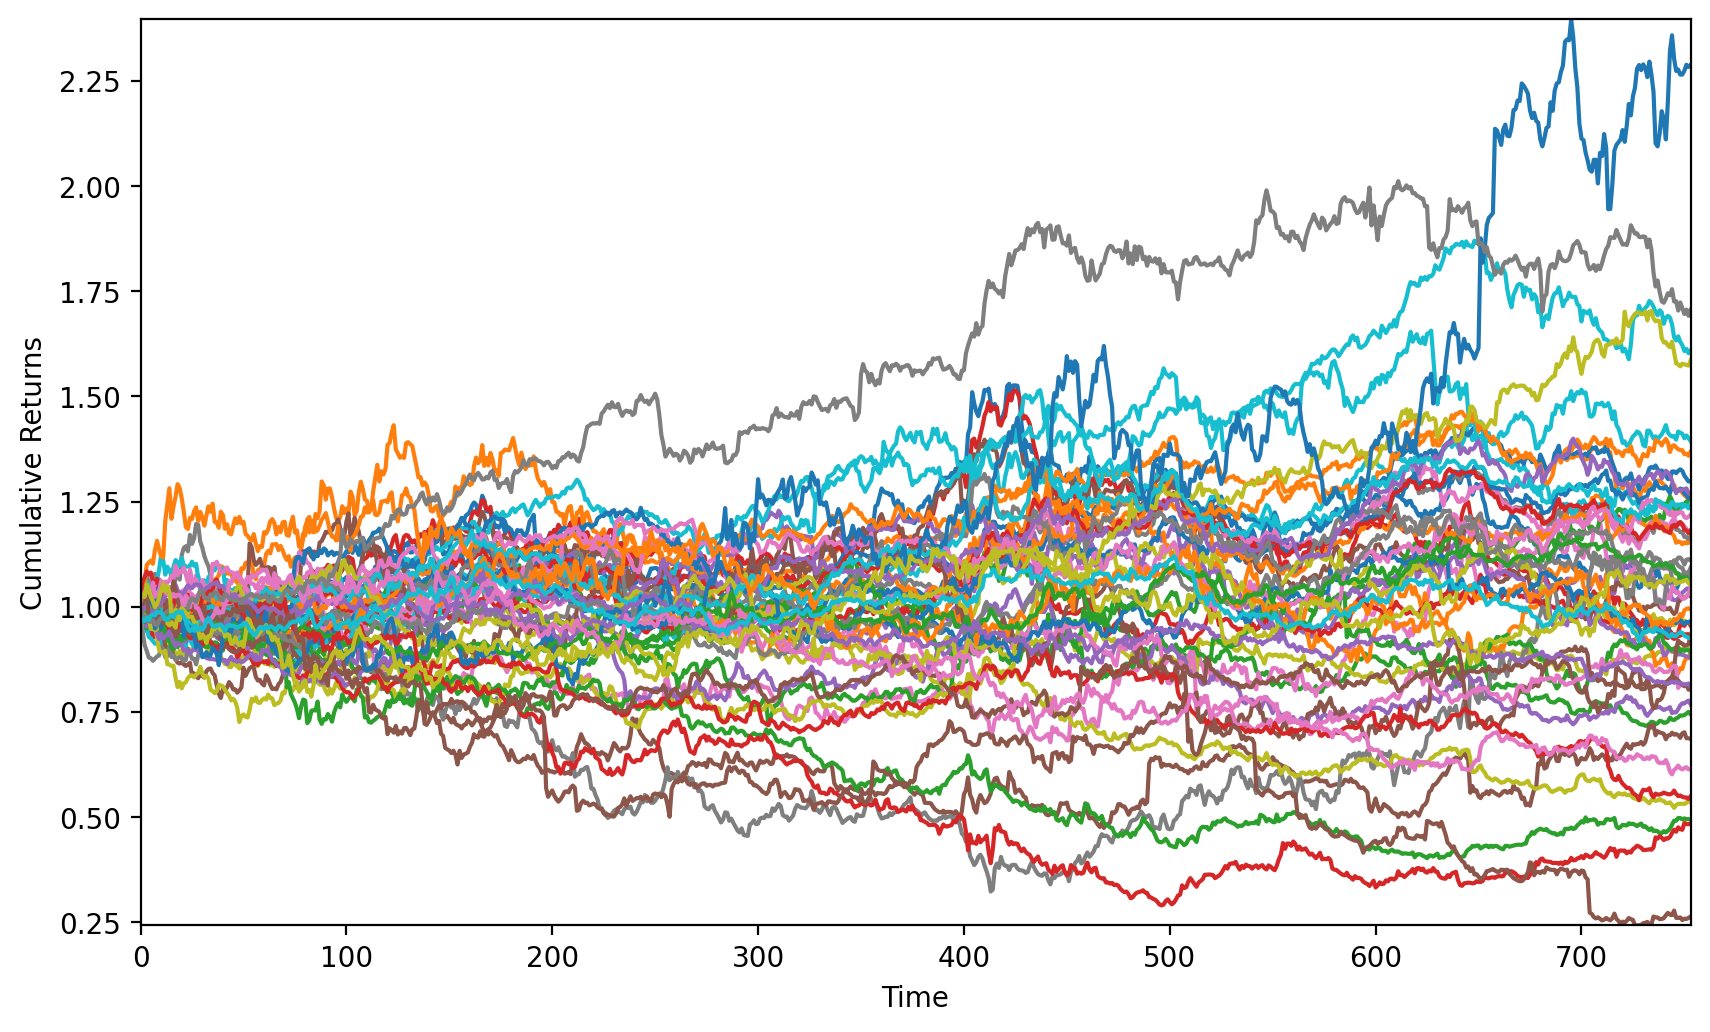
\includegraphics[width=0.8\textwidth]{images/cumulative_returns_qrt_timeseries_data.png}
%     \caption{Cumulative Returns for Daily Returns Time Series}
%     \label{fig:cumulative_returns}
% \end{figure}
% \begin{figure}[htbp]
%   \centering
%   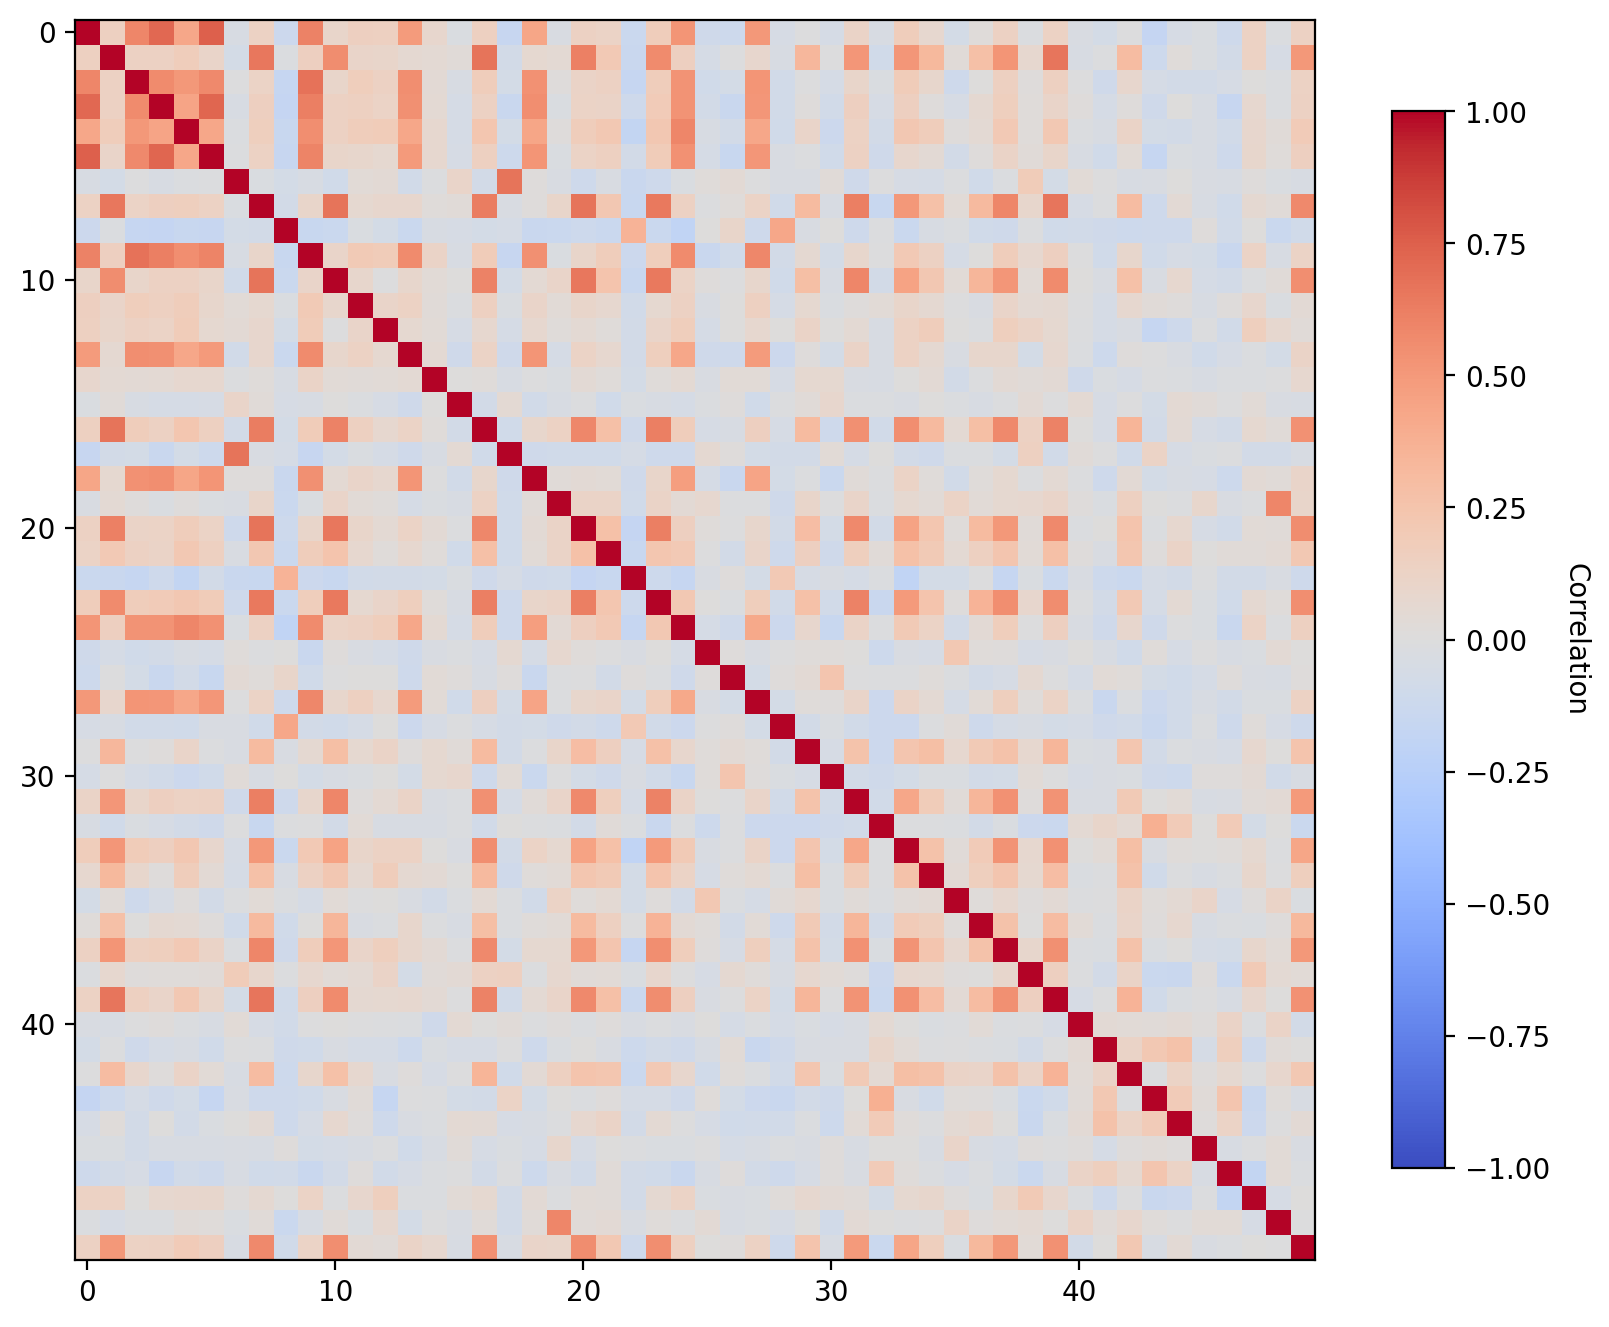
\includegraphics[width=0.9\textwidth]{images/correlation_matrix_50by50_timeseries_qtr_data.png}
%   \caption{Correlation Matrix for returns of 50 time series}
%   \label{fig:corr_matrix_ts_qrt_data}
% \end{figure}

\begin{figure}[H]
    \centering
    \begin{minipage}[t]{0.5789\textwidth}
        \centering
        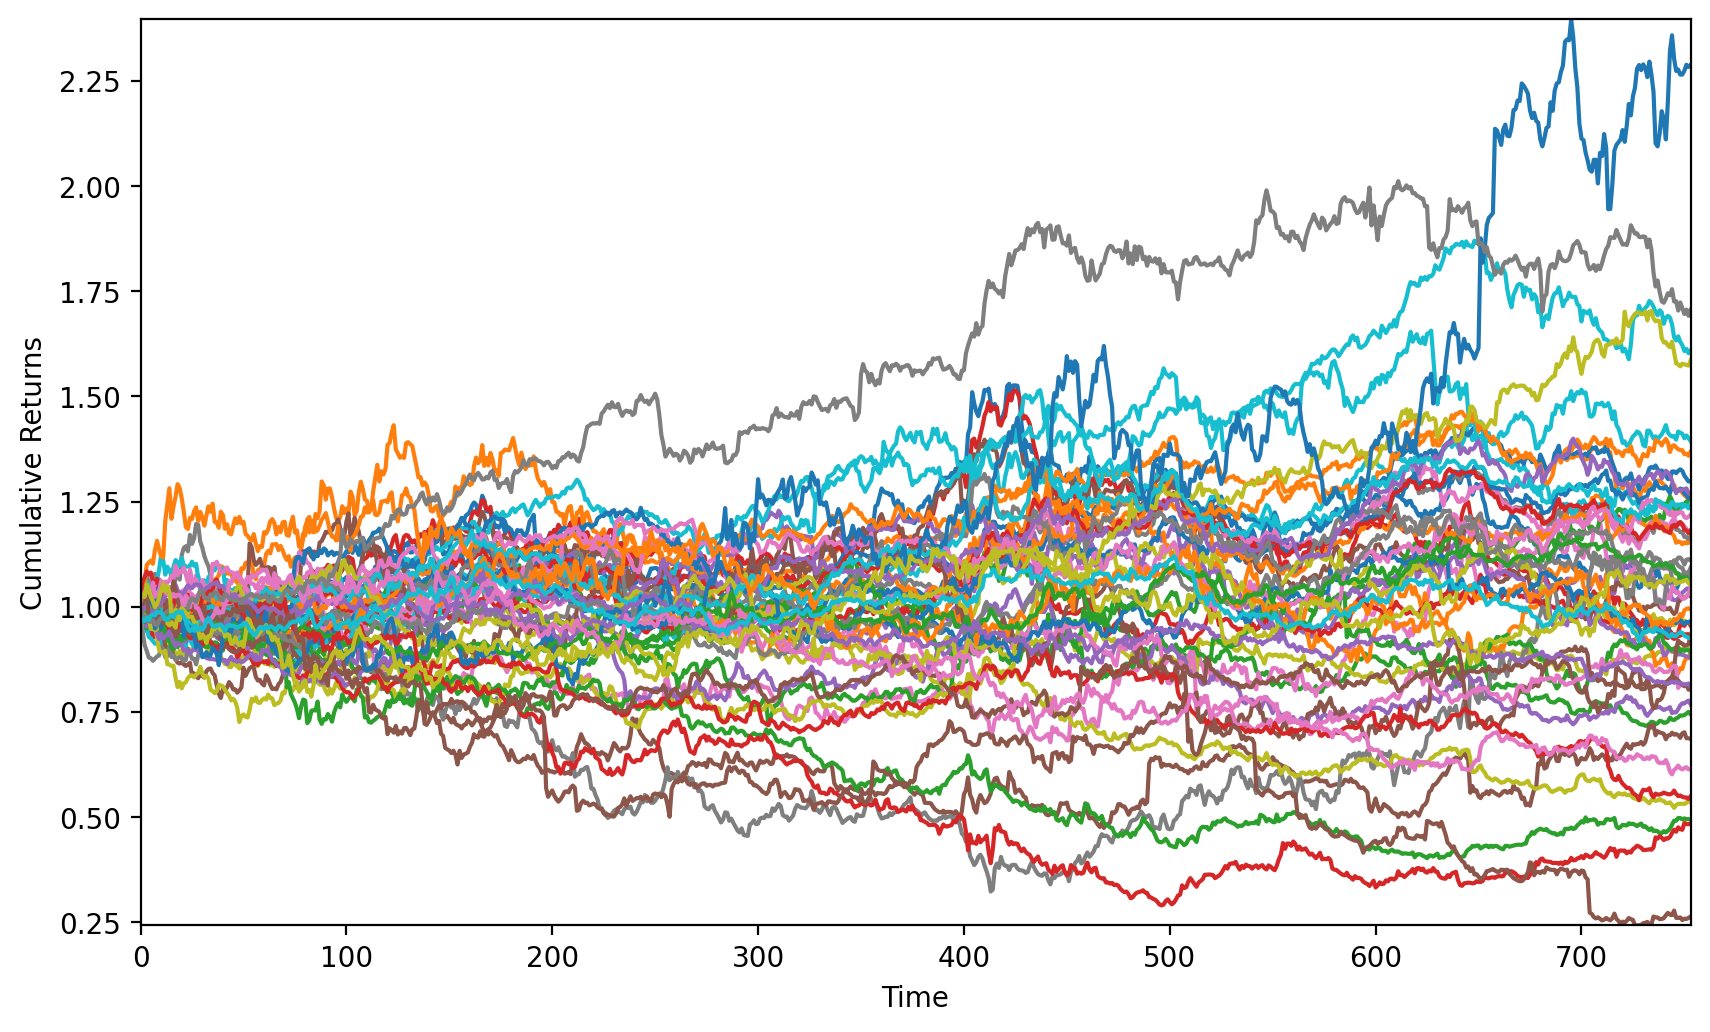
\includegraphics[width=\textwidth]{images/cumulative_returns_qrt_timeseries_data.png}
        \captionsetup{font=tiny}
        \caption{Cumulative Returns for Daily Returns Time Series}
        \label{fig:cumulative_returns}
    \end{minipage}%
    \begin{minipage}[t]{0.4211\textwidth}
        \centering
        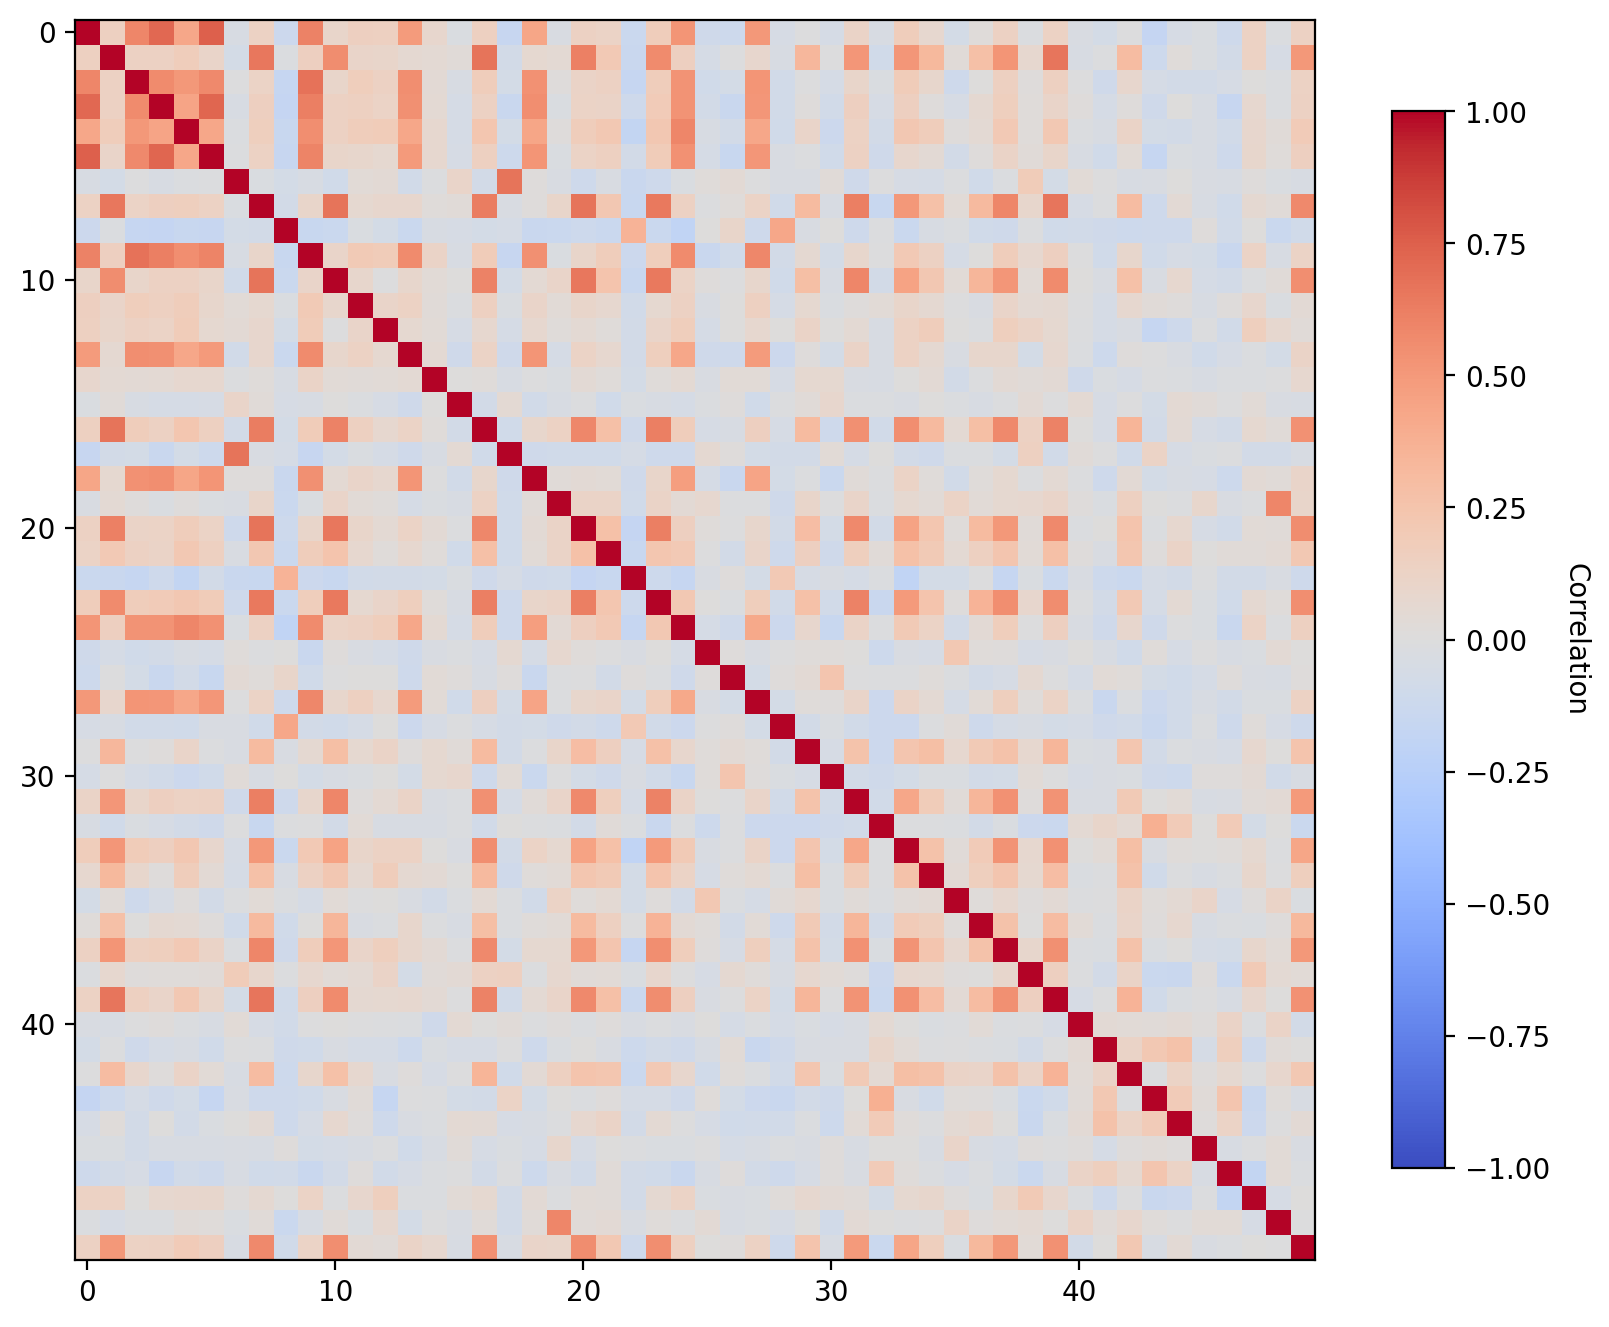
\includegraphics[width=\textwidth]{images/correlation_matrix_50by50_timeseries_qtr_data.png}
        \captionsetup{font=tiny}
        \caption{Correlation Matrix of Daily Returns}
        \label{fig:corr_matrix_ts_qrt_data}
    \end{minipage}
\end{figure}
\begin{figure}[H]
  \centering
  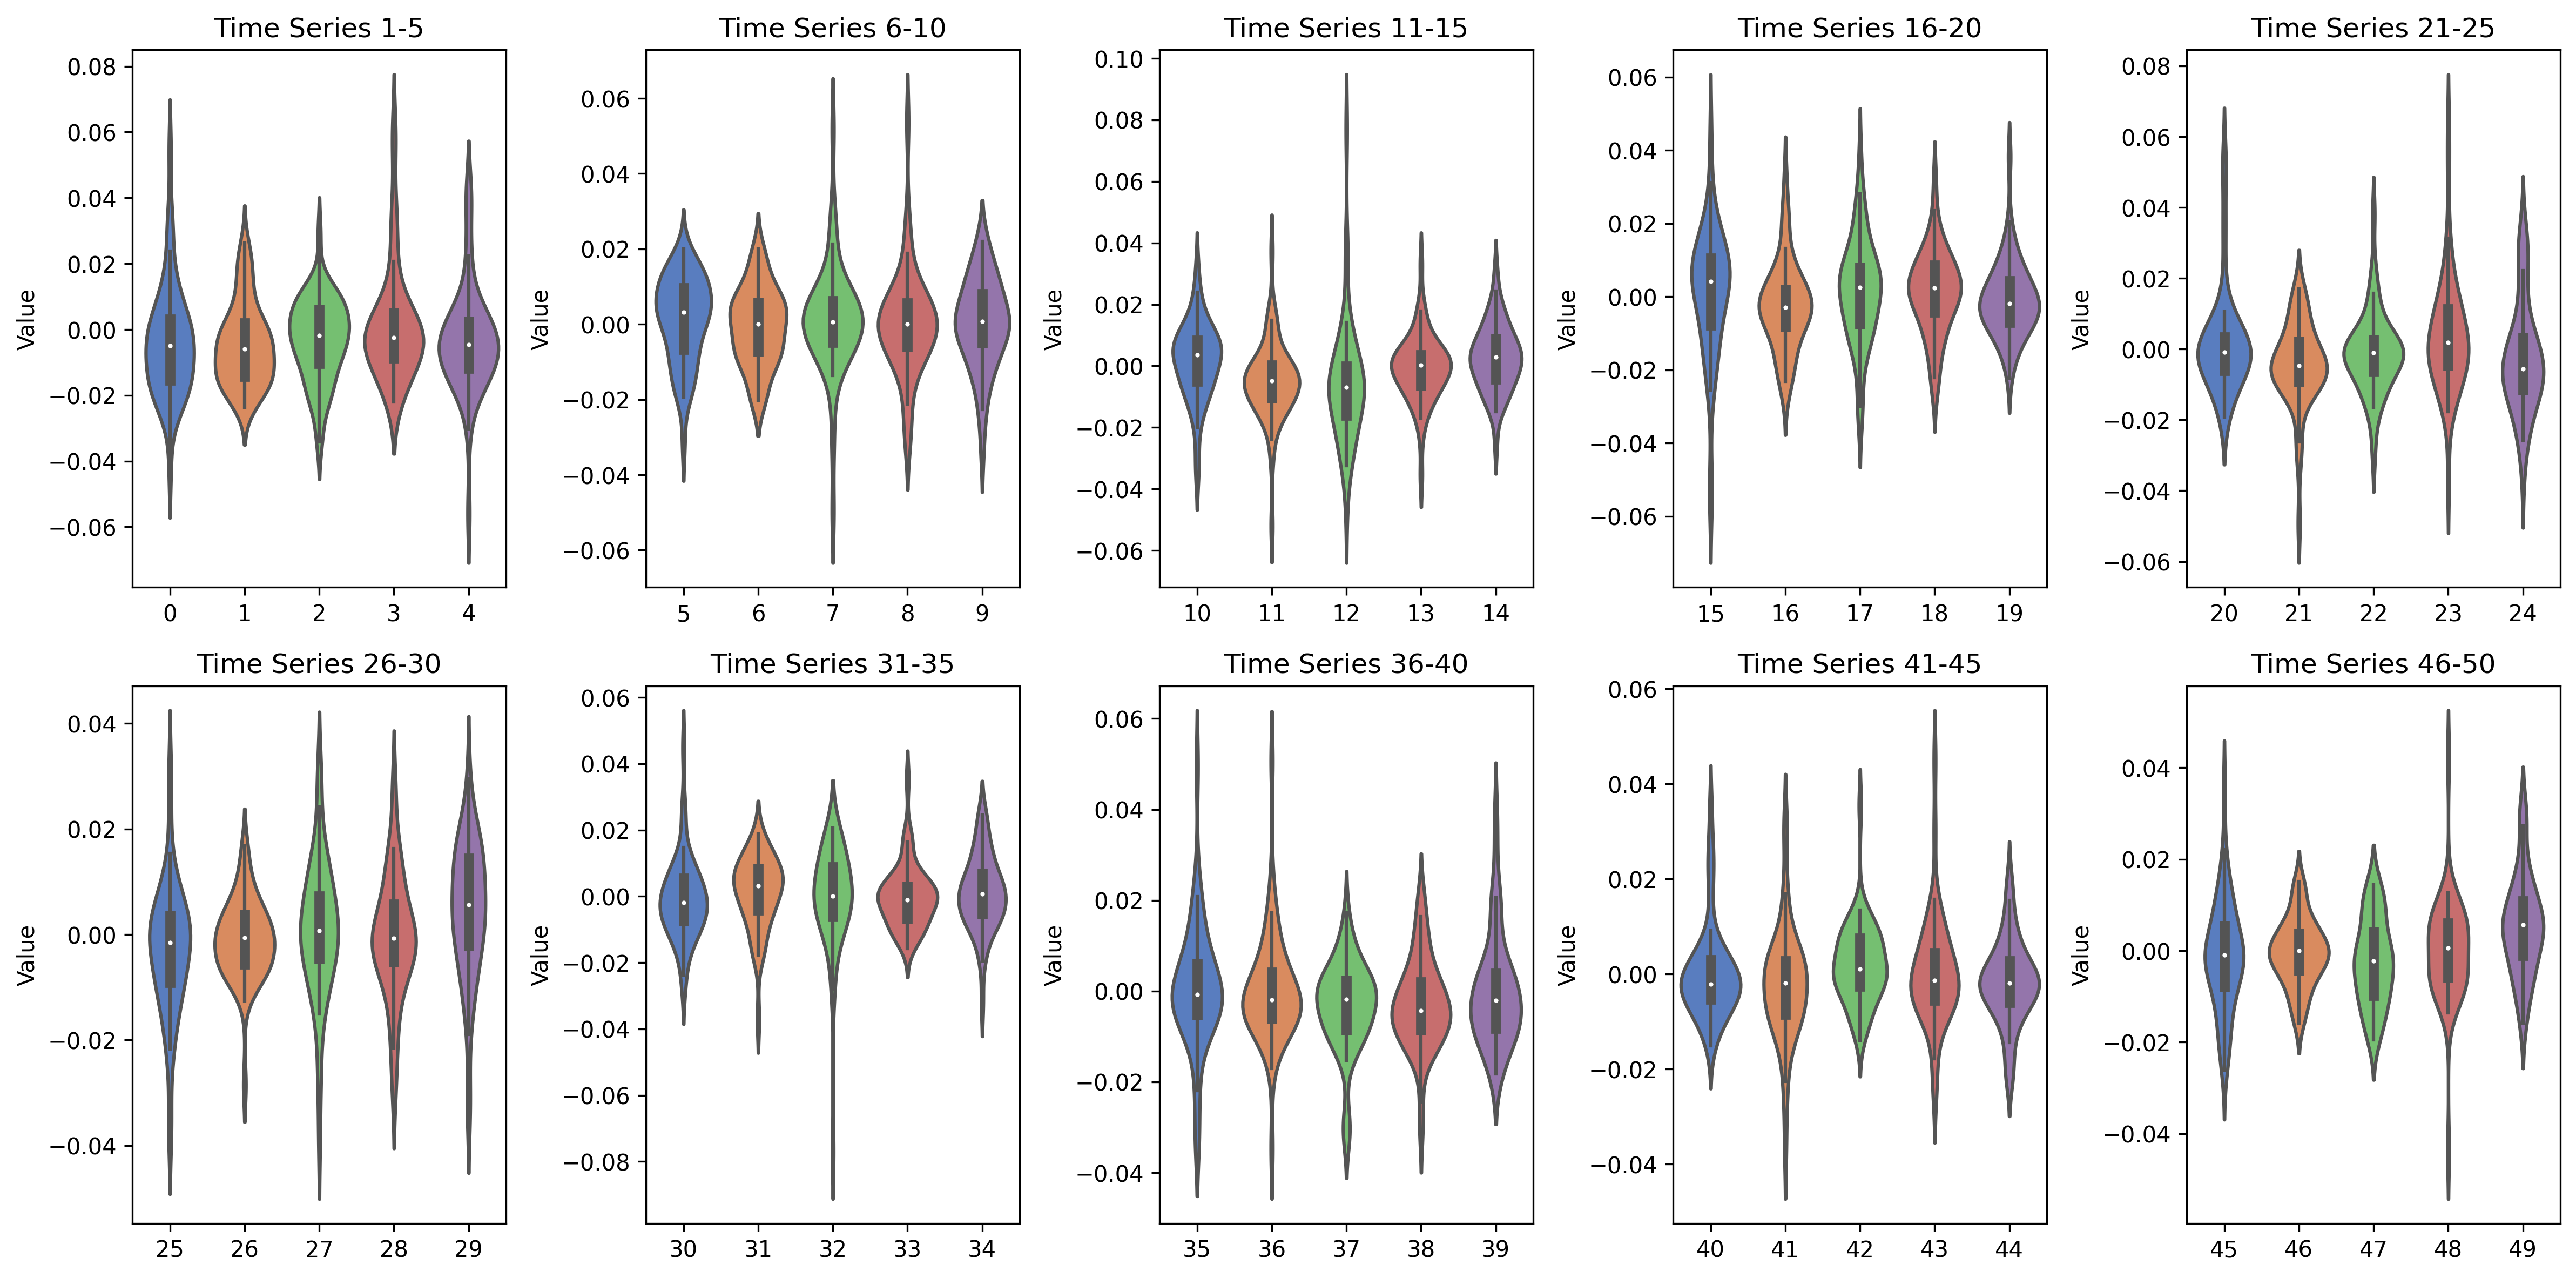
\includegraphics[width=\textwidth]{images/violin_plots_50_timeseries.png}
  \caption{Violin Plots for 50 Time Series}
  \label{fig:violin_plots}
\end{figure}

\level{2}{Results}

Since we have two objectives and one important condition, namely $R = \mathcal{R}_{\beta, A}$, $L = \mathcal{L}_{\beta, A}$, and $O = \frac{1}{2}||AA^\top -I||^2_F$, we will use their negative logarithms for the purpose of comparing the methods and deriving the statistics, as $L$ and $O$ are losses. Note that the higher the value of $R$, $-log(L)$, and $-log(O)$, the better the solution/method.

\level{3}{Baseline Method}
We implemented the baseline method and executed it for $N=10000$ (i.e., $\mathcal{A}_{0}[10000]$). For the plots below color of the point indicates it's $-log(L)$ value. We observe that all solutions have a high value of $-log(L)$, which appears to be bounded due to natural variation in the data. Additionally, the solutions are symmetrically distributed over $R$, but exhibit a skewed distribution over the values of $-log(O)$.
\begin{figure}[H]
    \centering
    \begin{minipage}[t]{0.45\textwidth}
        \centering
        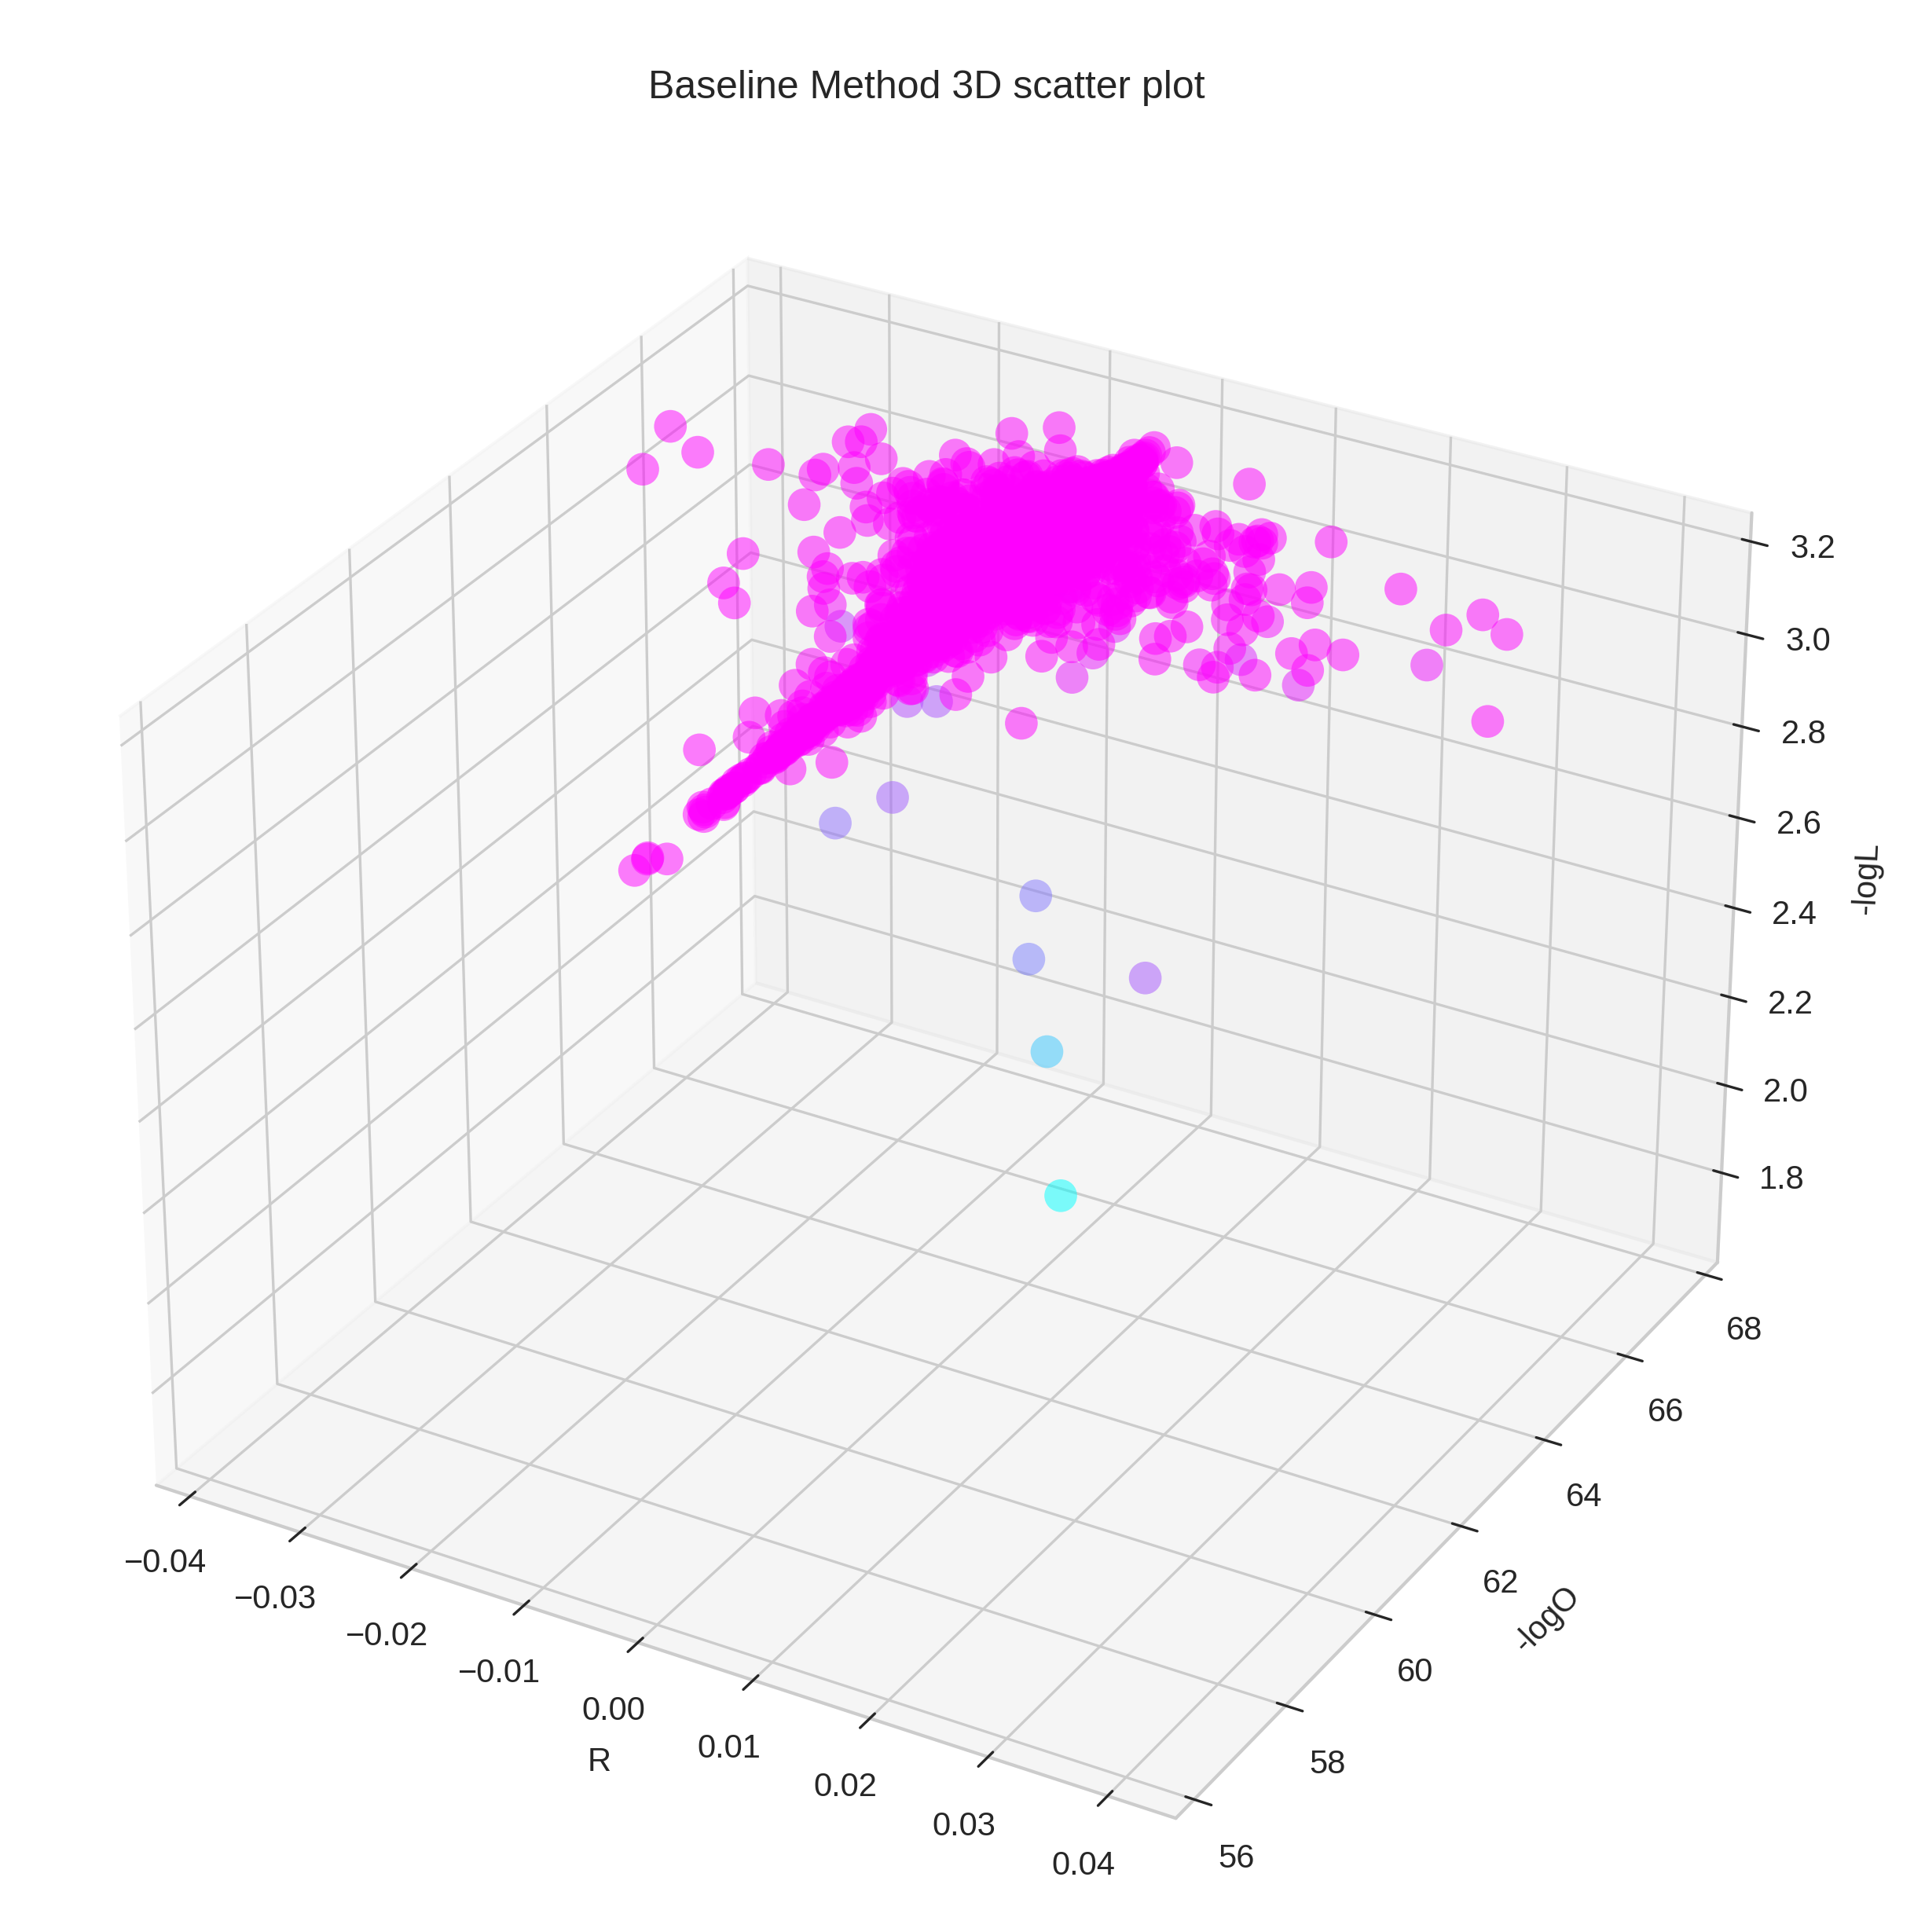
\includegraphics[width=\textwidth]{images/1-Baseline Method 3D scatter plot.png}
        \captionsetup{font=tiny}
        \caption{3D Scatter Plot : Baseline Method}
        \label{fig:cumulative_returns}
    \end{minipage}%
    \begin{minipage}[t]{0.5511\textwidth}
        \centering
        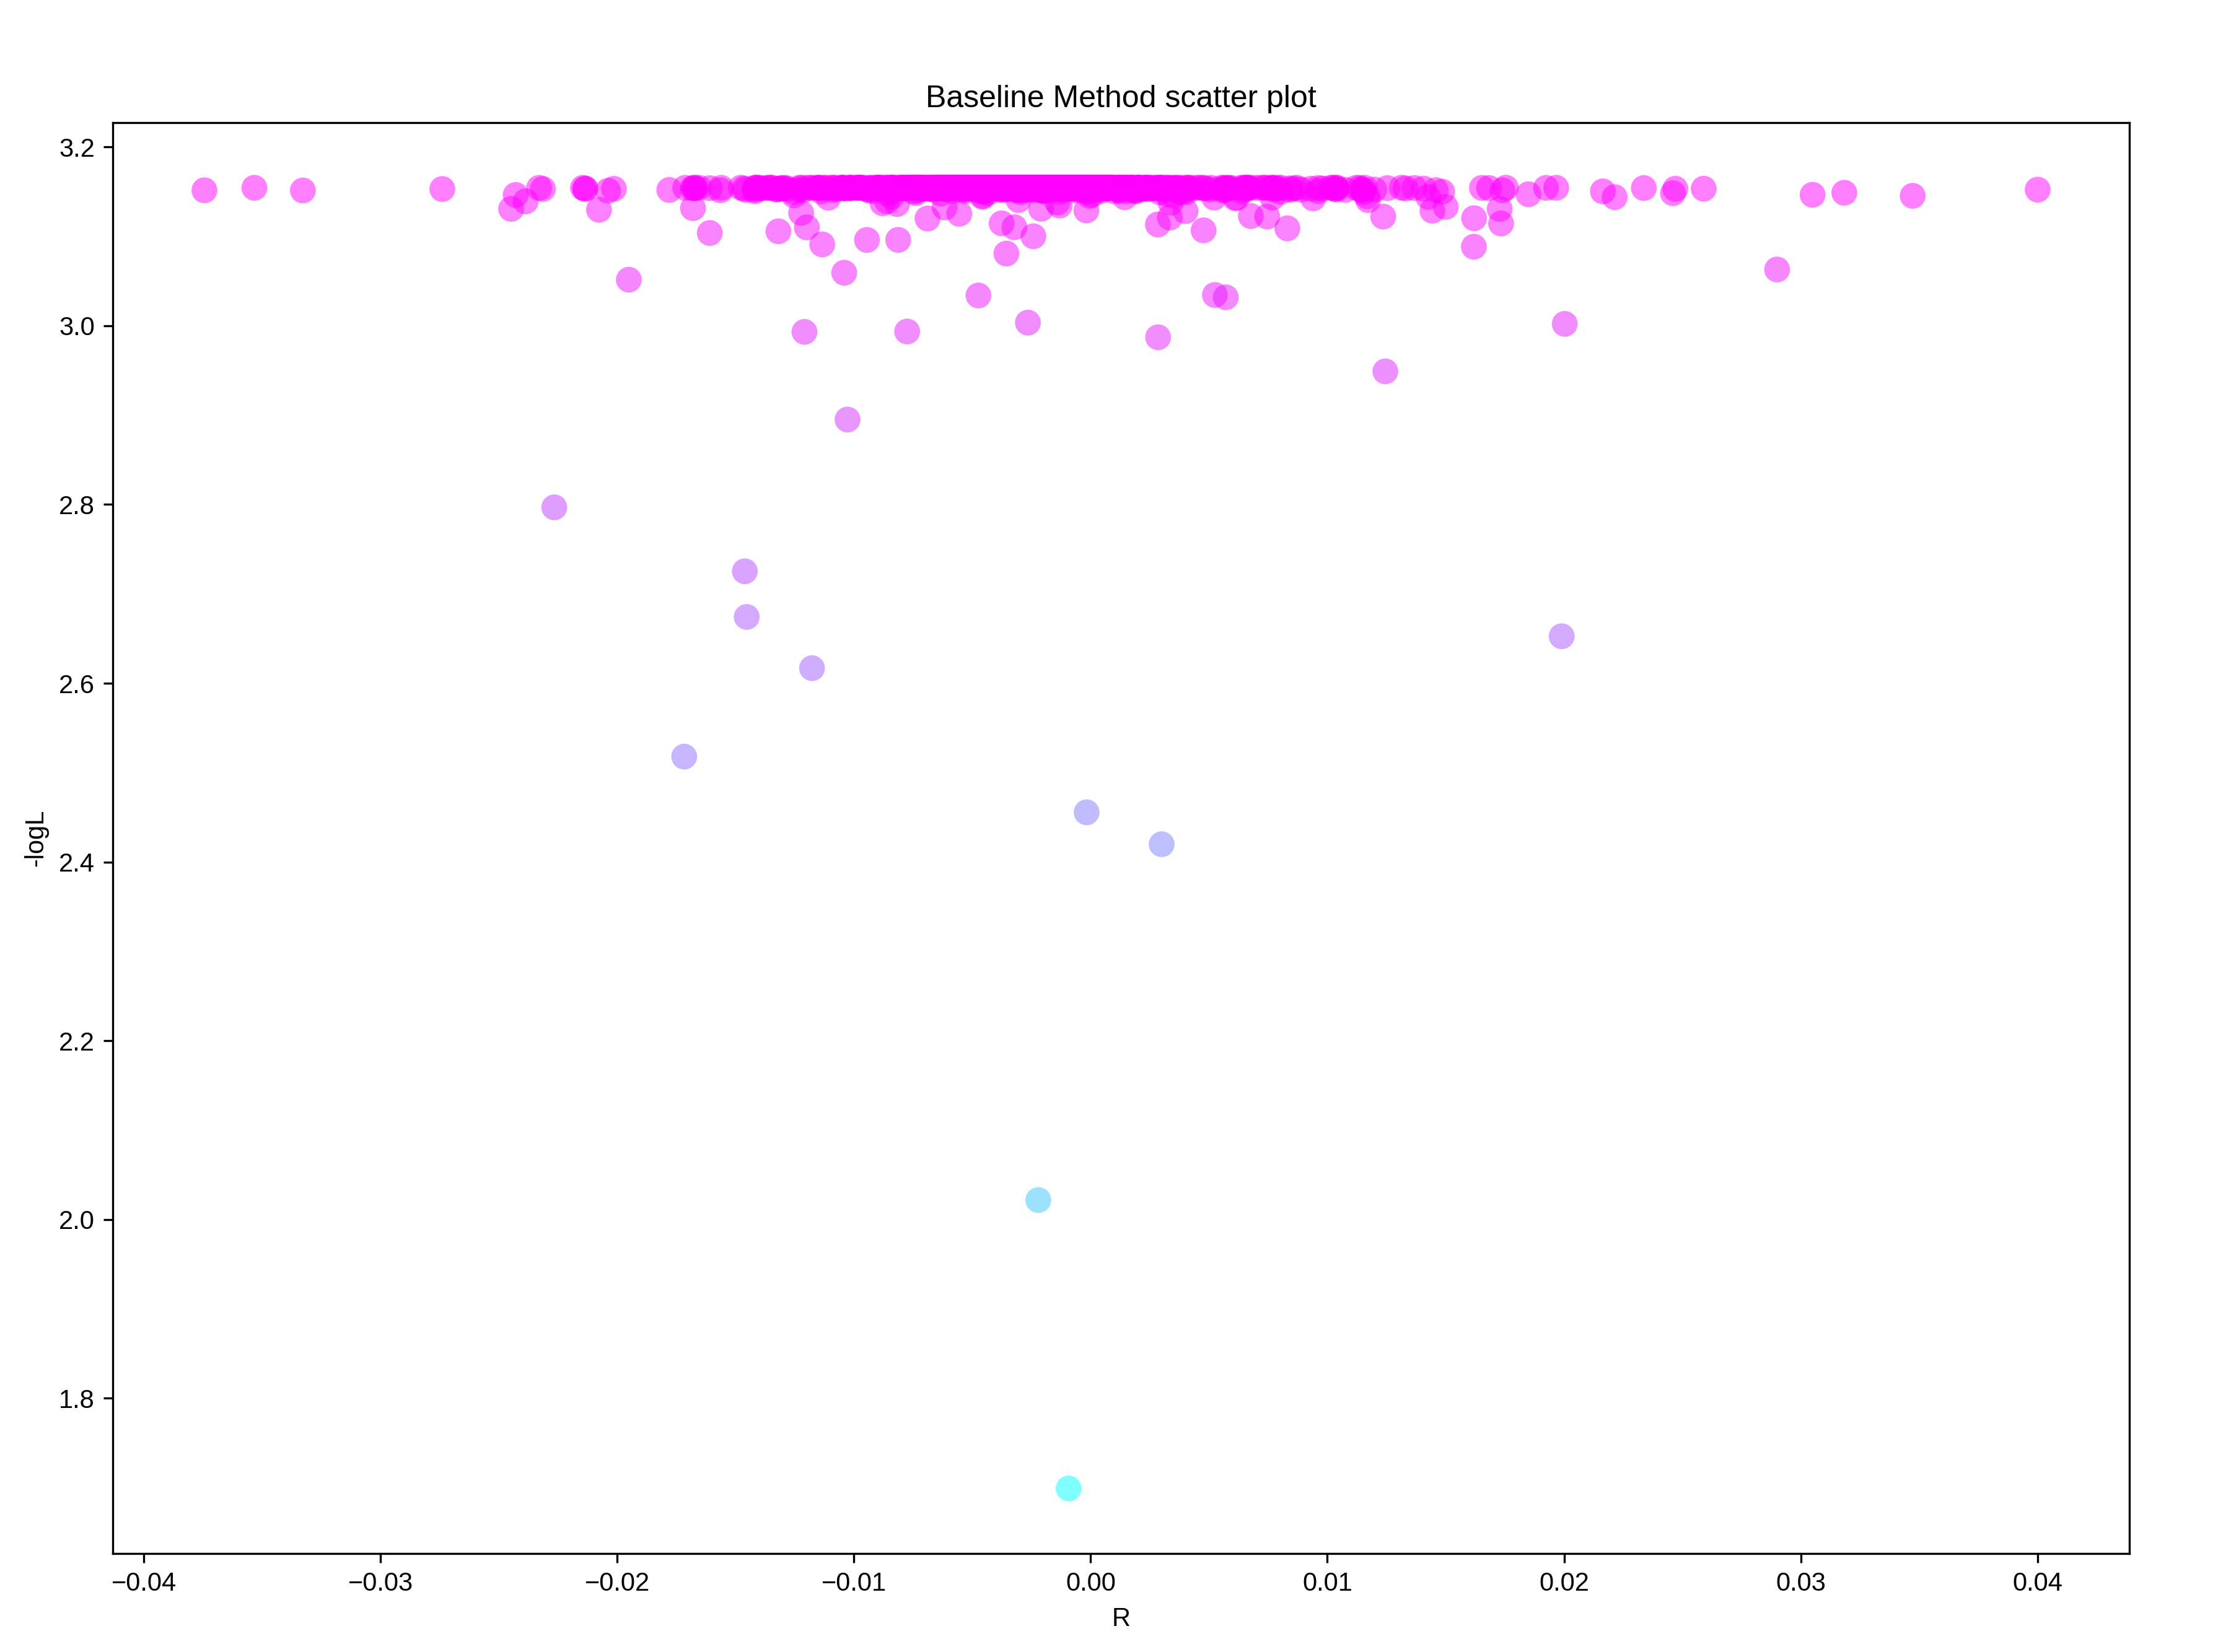
\includegraphics[width=\textwidth]{images/1-Baseline Method scatter plot_R_vs_-logL.png}
        \captionsetup{font=tiny}
        \caption{2D $(R,-log(L))$ Scatter Plot : Baseline Method}
        \label{fig:corr_matrix_ts_qrt_data}
    \end{minipage}
\end{figure}
\level{3}{OPI Method : Type 1} 
To get better statistical result we ran the method multiple times with value of $N$ set to  $1000$. $\mathcal{A}_{1}[1000,\mathcal{U}^{1}_{A},\mathcal{U}^{1}_{\beta}]$, we are using $\mathcal{U}^{1}_{A}[(100,0.01,0.3,0.3,0.3)]$ to update $A$ and $\mathcal{U}^{1}_{\beta}[(100,0.01,0.5,0.5)]$ to update $\beta$.  We observe that all solution attempts converge to the same point in $(R,-log(L))$, with initial updates being large but decreasing over time. Additionally, this method is able to overcome the problem of local minima in one dimension through the presence of better minima in another dimension.
\begin{figure}[H]
    \centering
    \begin{minipage}[t]{0.45\textwidth}
        \centering
        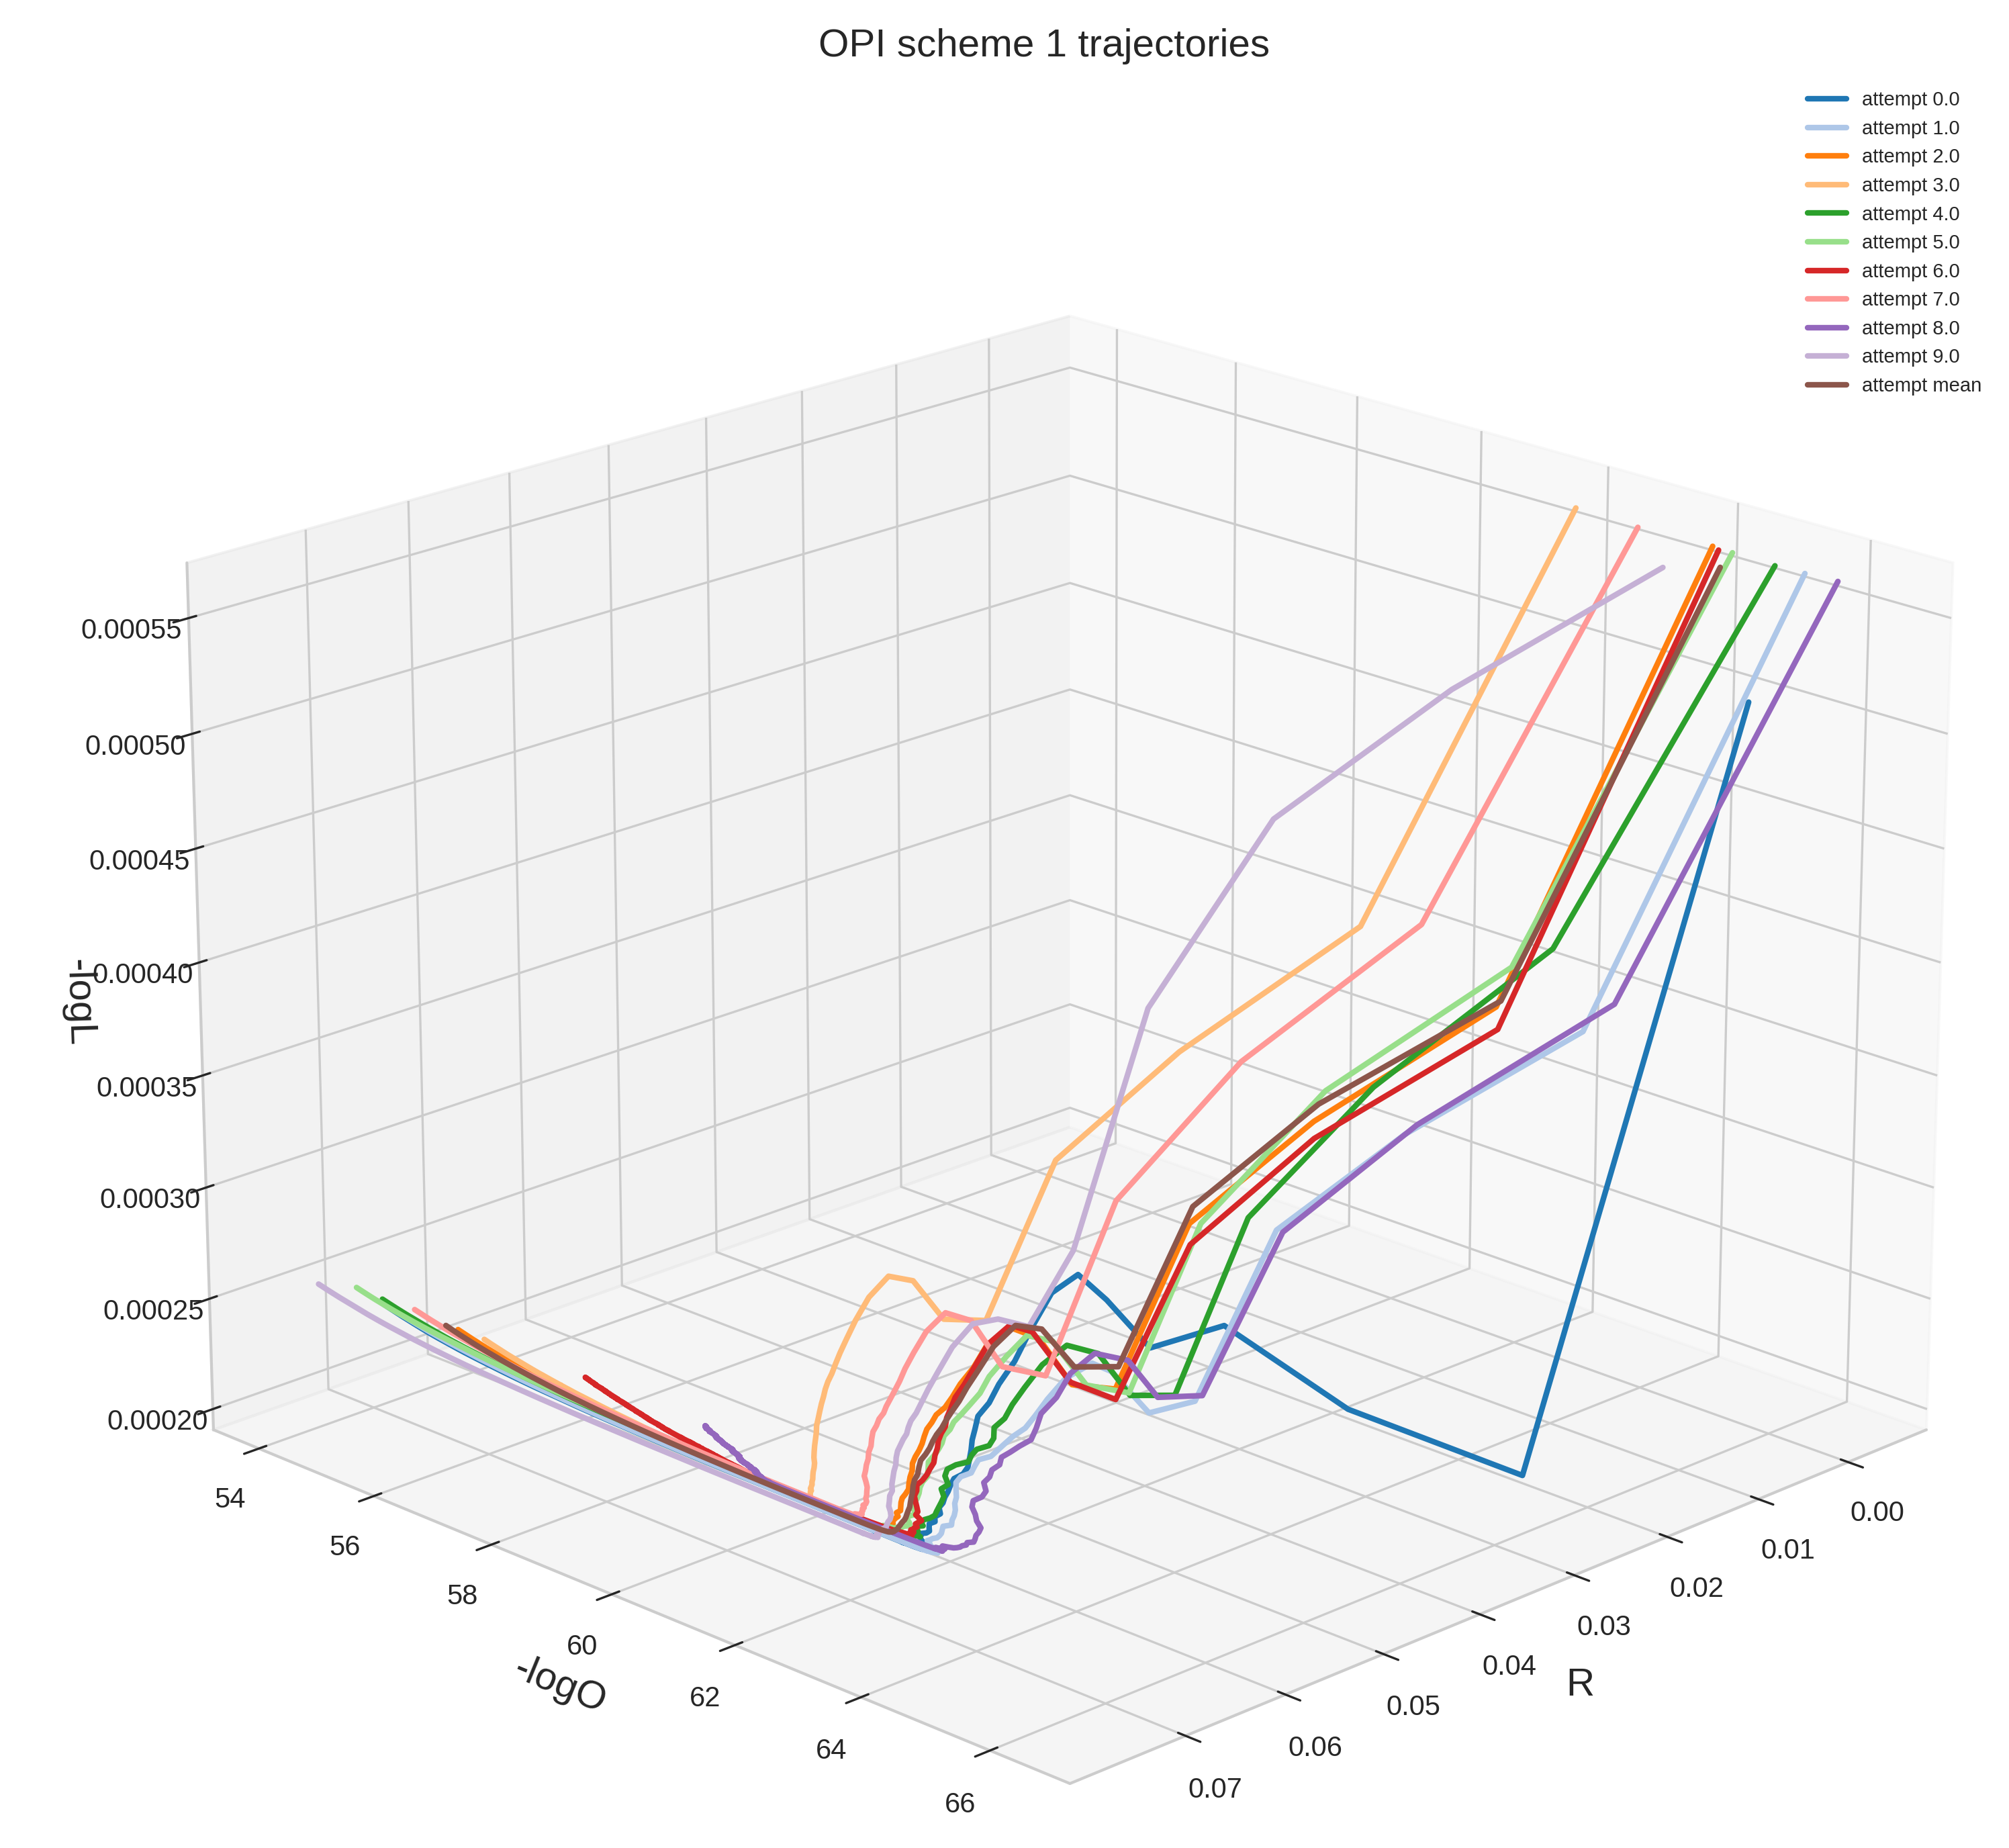
\includegraphics[width=\textwidth]{images/OPI scheme 1 mean trajectory.png-.png}
        \captionsetup{font=tiny}
        \caption{3D Trajectory Line Plot : OPI Method Type 1}
        \label{fig:cumulative_returns}
    \end{minipage}%
    \begin{minipage}[t]{0.5511\textwidth}
        \centering
        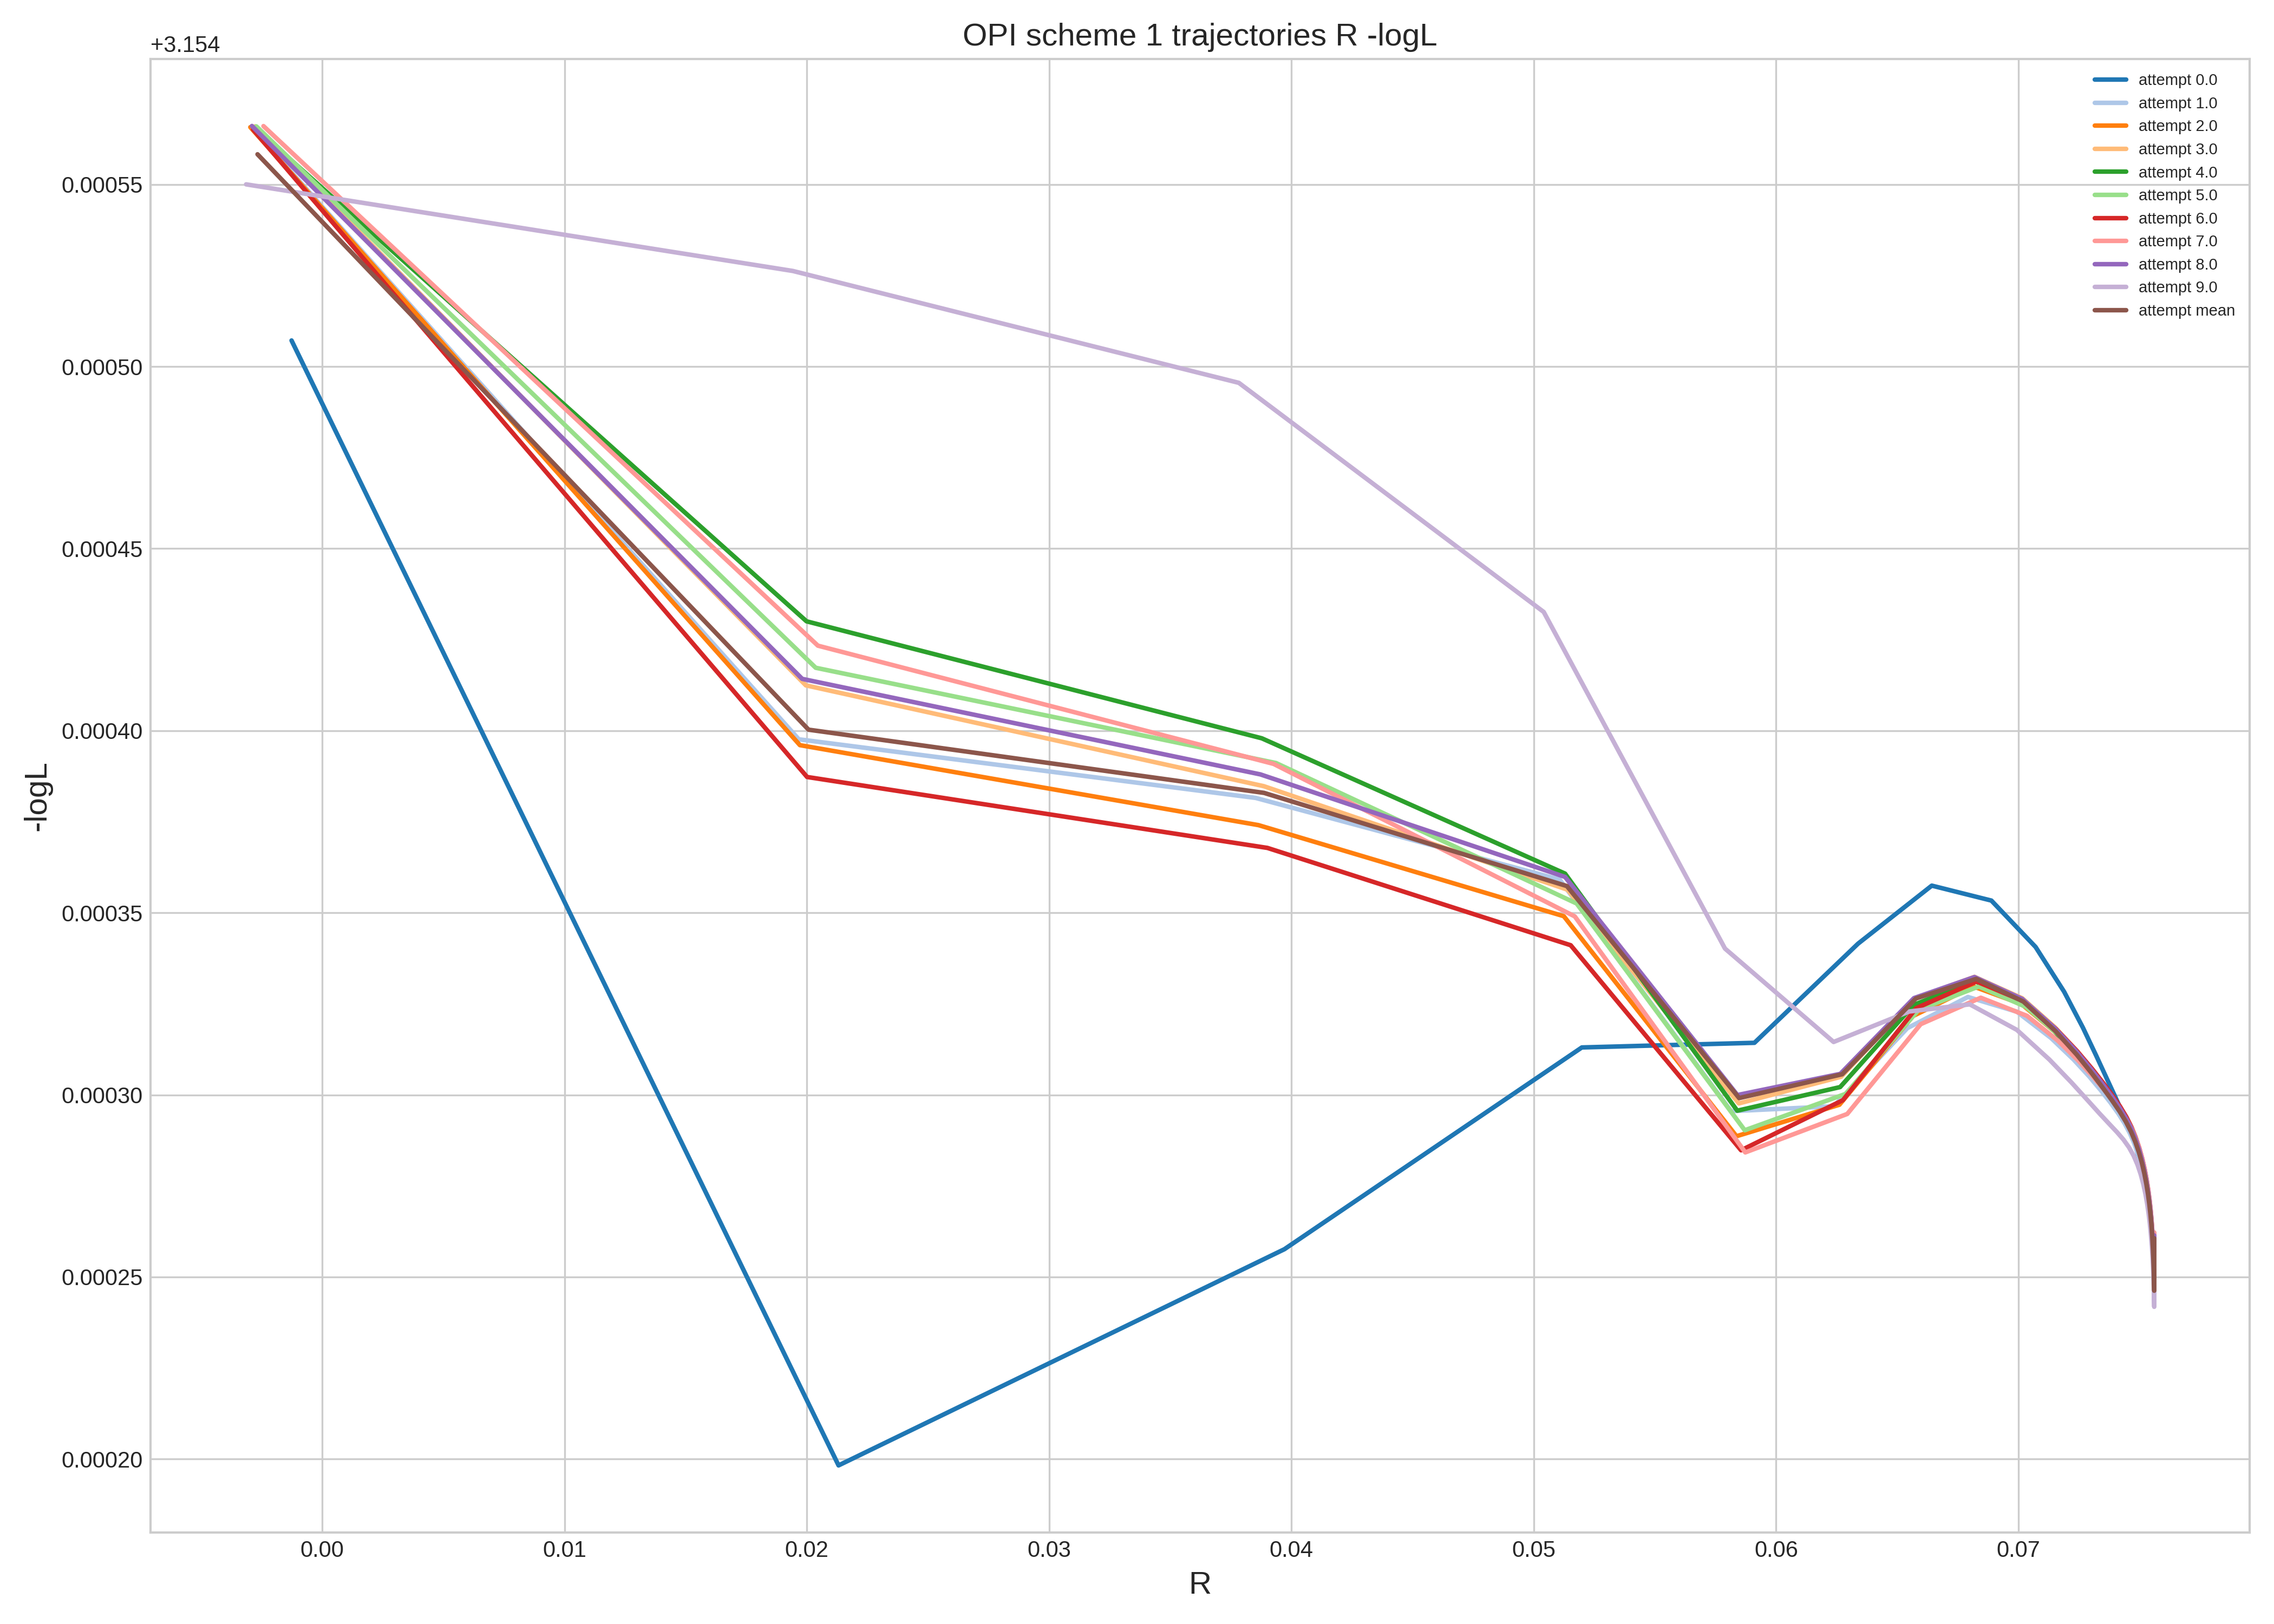
\includegraphics[width=\textwidth]{images/OPI scheme 1 trajectories R -logL.png}
        \captionsetup{font=tiny}
        \caption{2D $(R,-log(L))$ Trajectory Line Plot : OPI Method Type 1}
        \label{fig:corr_matrix_ts_qrt_data}
    \end{minipage}
\end{figure}
\level{3}{OPI Method : Type 2}
To get better statistical result we ran the method multiple times with $N=1000$. This method uses $\mathcal{U}^{1}_{A}$ to update $A$ but $\mathcal{U}^{2}_{\beta}[(100,0.01,0.5,0.5,0.01)]$ to update $\beta$. We observe that this method updates the solutions non-smoothly, as it relies on regression to update $\beta$, which may result in the next update taking the value of $(R,-log(L),-log(O))$ to a distant point.
\begin{figure}[H]
    \centering
    \begin{minipage}[t]{0.45\textwidth}
        \centering
        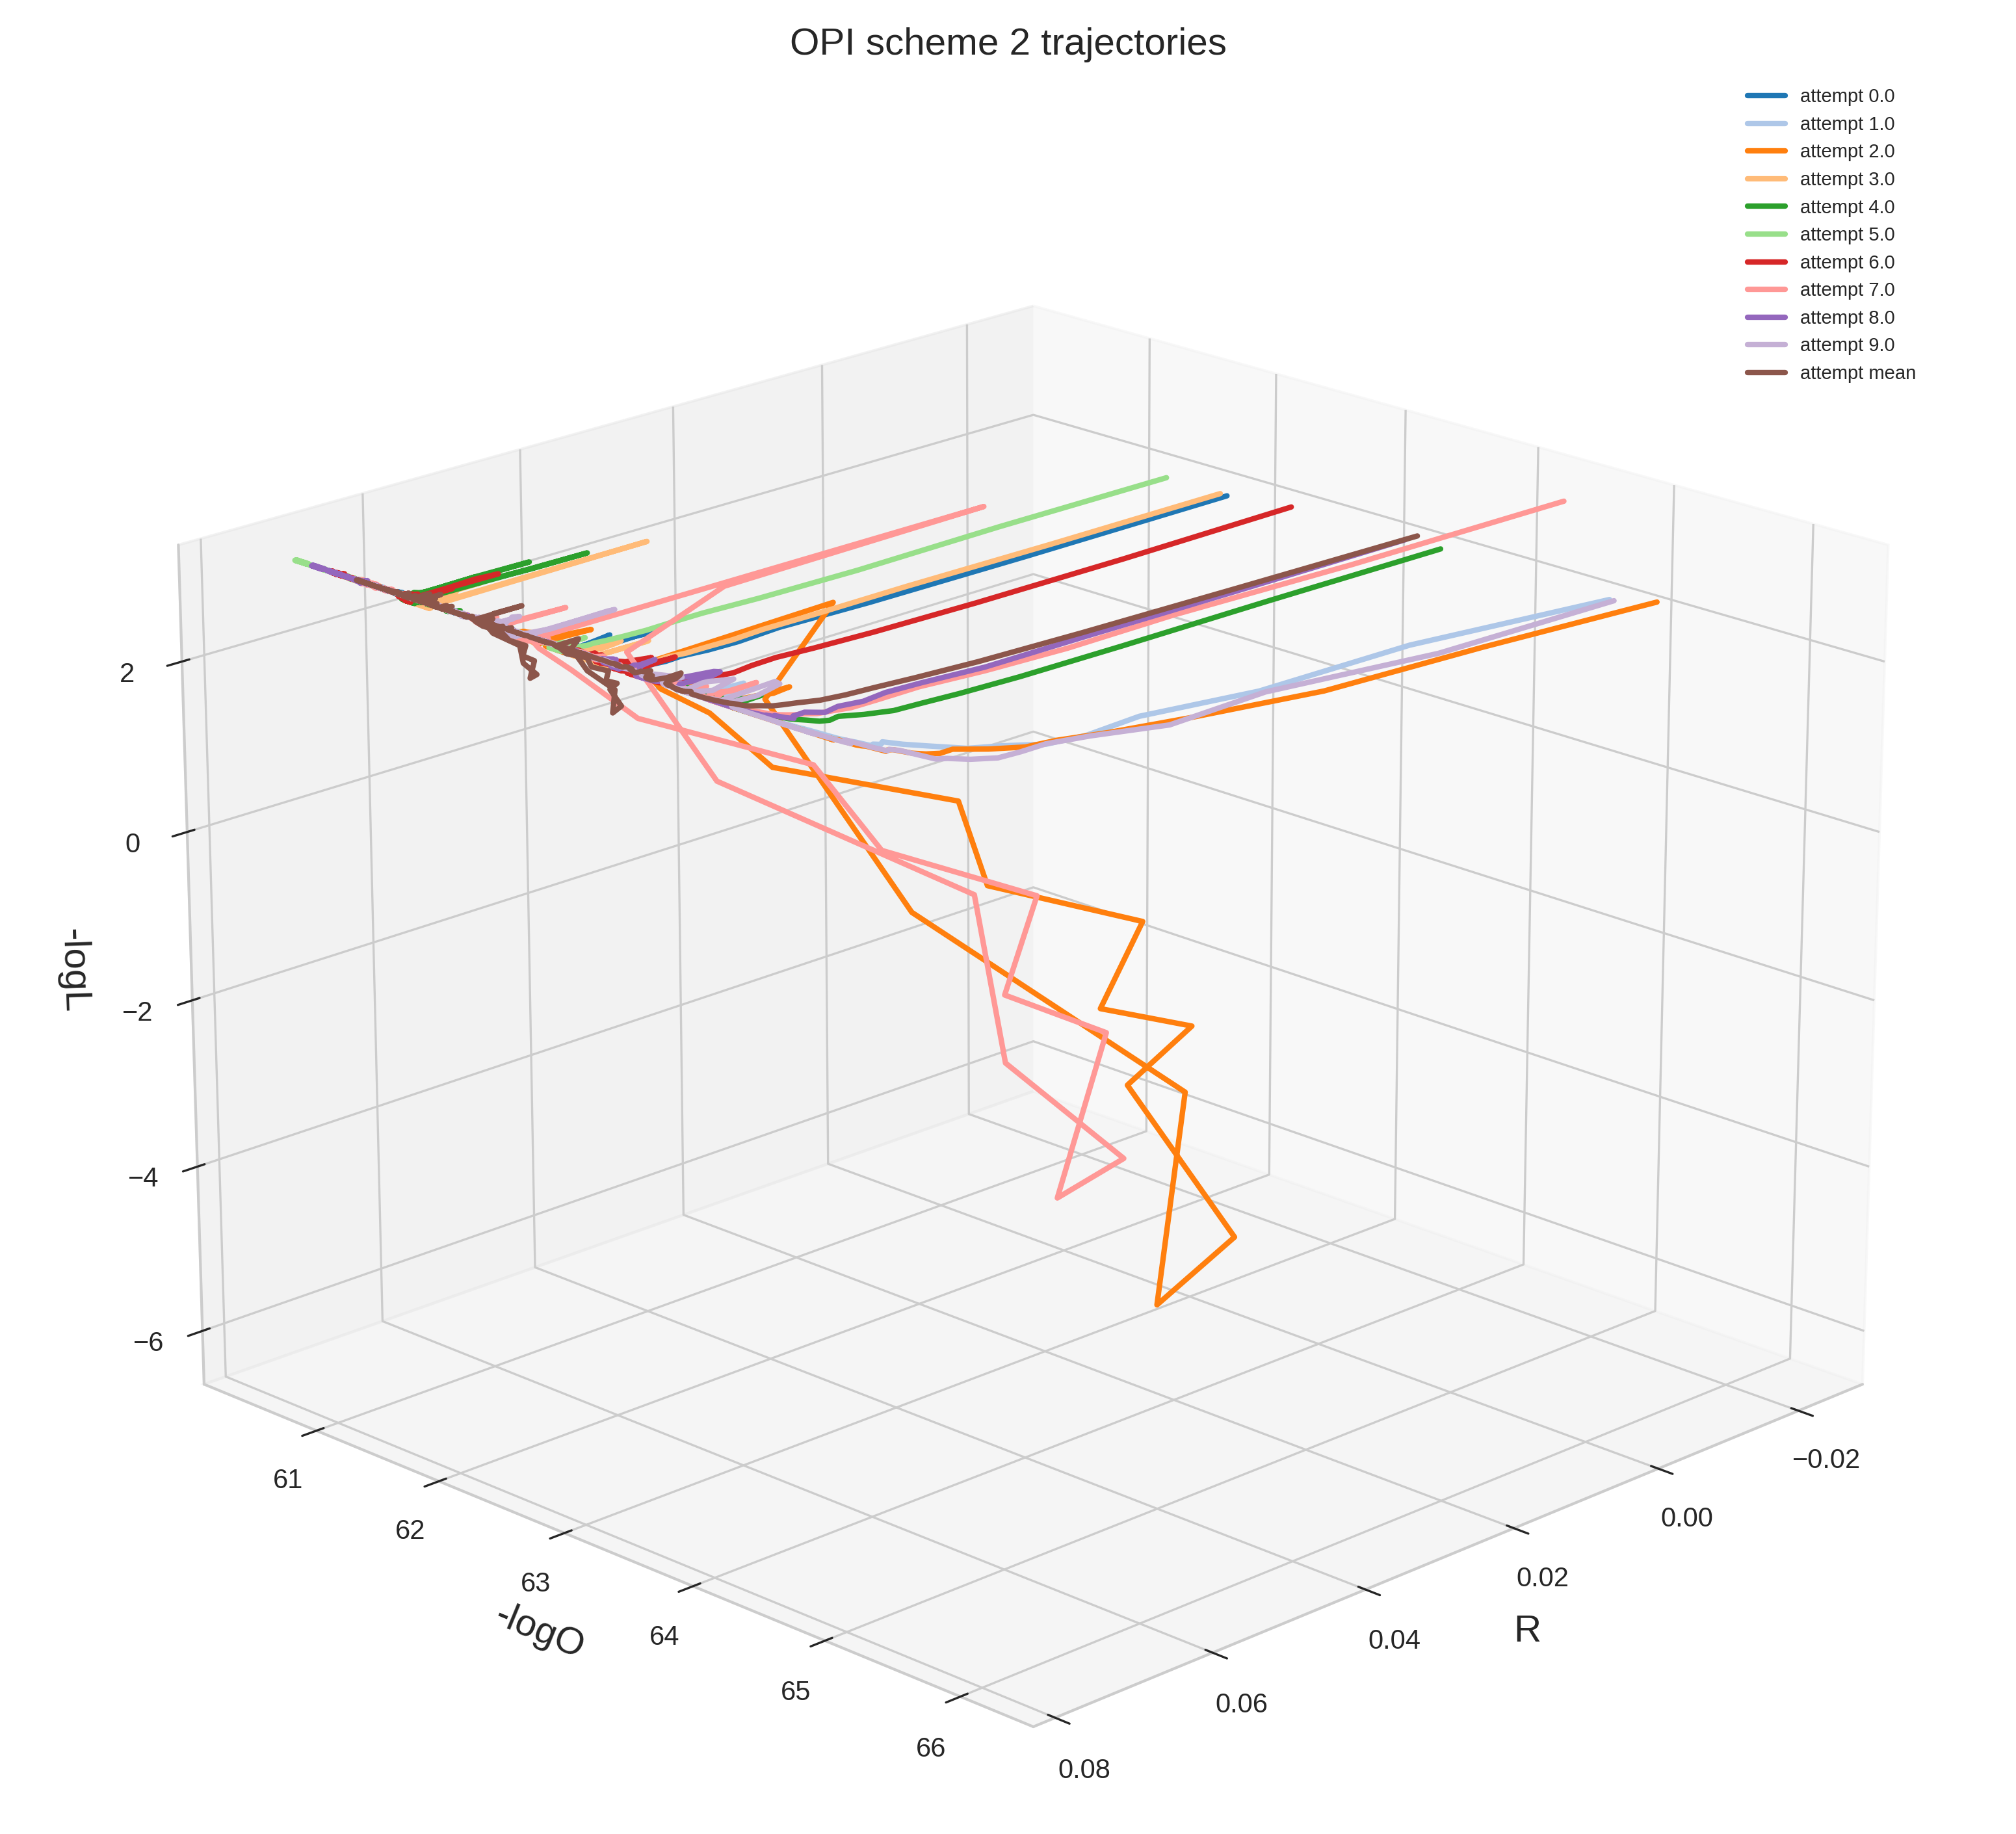
\includegraphics[width=\textwidth]{images/1-OPI scheme 2 mean trajectory.png}
        \captionsetup{font=tiny}
        \caption{3D Trajectory Line Plot : OPI Method Type 2}
        \label{fig:cumulative_returns}
    \end{minipage}%
    \begin{minipage}[t]{0.5511\textwidth}
        \centering
        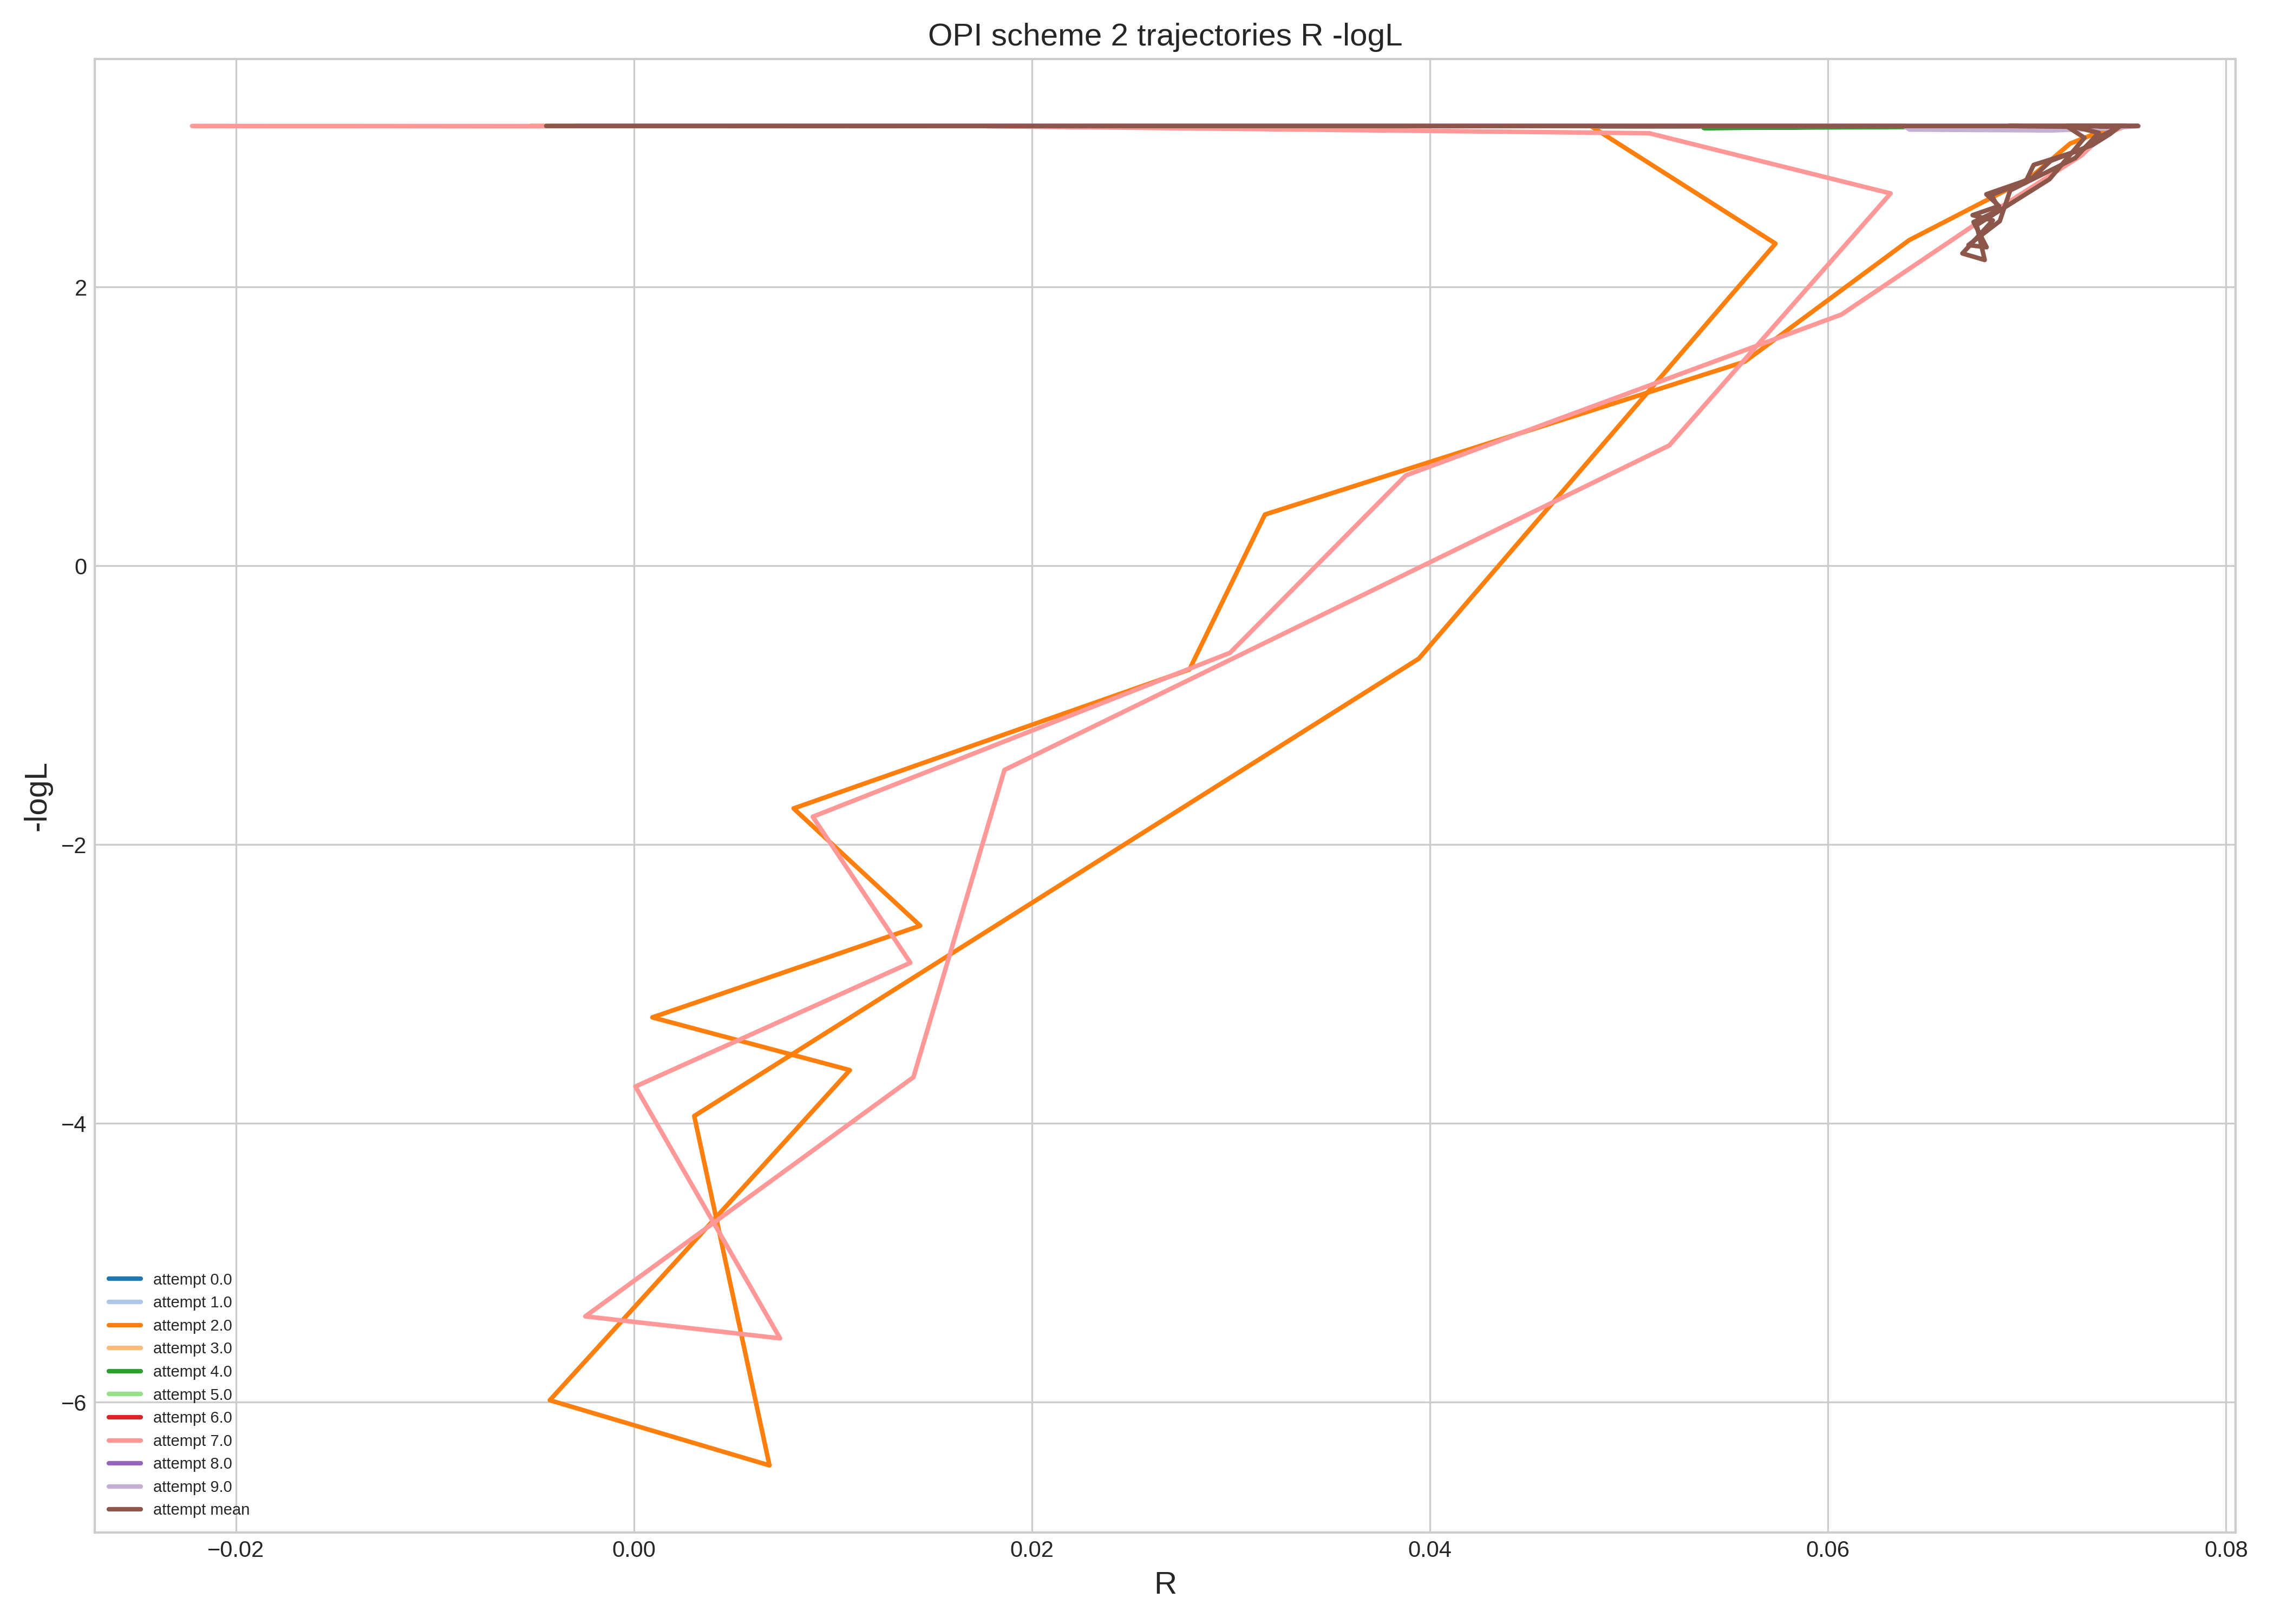
\includegraphics[width=\textwidth]{images/OPI scheme 2 trajectories R -logL.png}
        \captionsetup{font=tiny}
        \caption{2D $(R,-log(L))$ Trajectory Line Plot : OPI Method Type 2}
        \label{fig:corr_matrix_ts_qrt_data}
    \end{minipage}
\end{figure}
\level{3}{DOI Method : Type 1}
Here we use same internal methods as of OPI Type 1, but since this method relaxes $A\in \mathcal{O}^{k}_{d}$ to $A\in \mathbb{R}^{d\times k}$ we use $\mathcal{U}^{1}_{O}[100,0.01,0.3,0.3,0.3]$ to bring it back in $\mathcal{O}^{k}_{d}$. Same as before to get better statistical result we ran the method multiple times with $N=1000$. This method converges to a point with decreasing update size, but the generated solutions do not consider the condition $A\in \mathcal{O}^{k}_{d}$, resulting in non-smooth updates.
\begin{figure}[H]
    \centering
    \begin{minipage}[t]{0.45\textwidth}
        \centering
        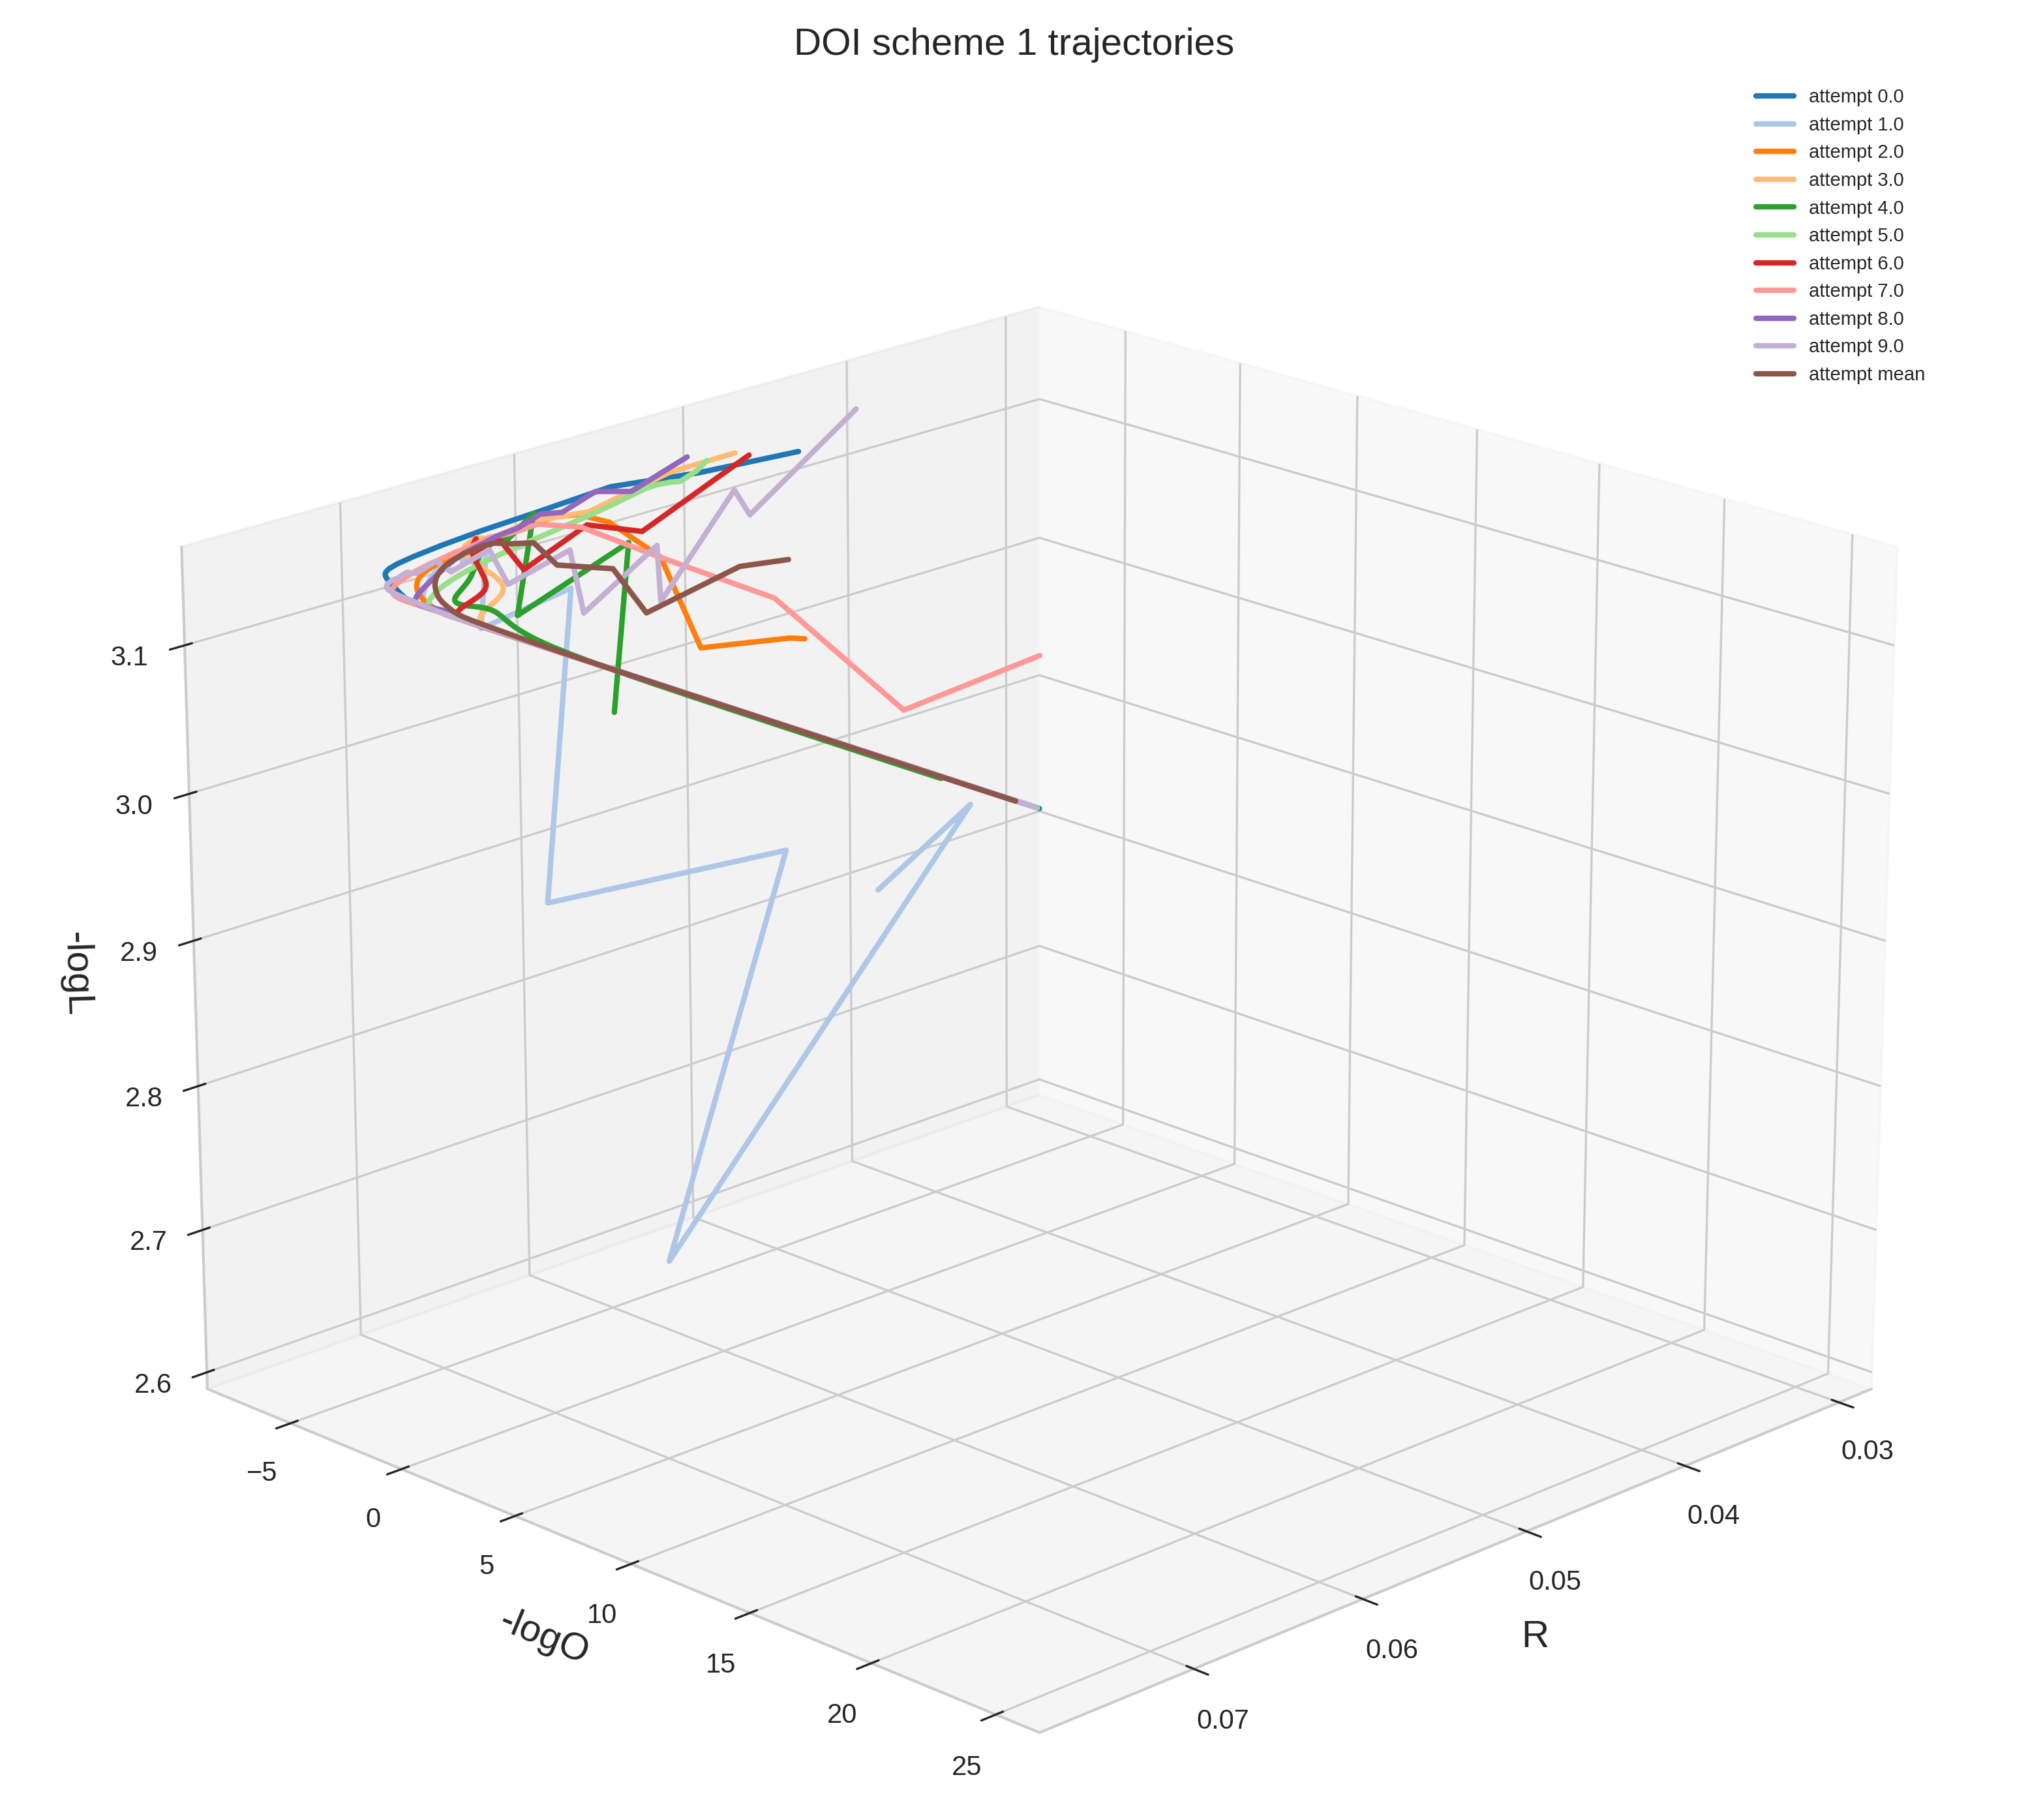
\includegraphics[width=\textwidth]{images/1-DOI scheme 1 mean trajectory.png}
        \captionsetup{font=tiny}
        \caption{3D Trajectory Line Plot : DOI Method Type 1}
        \label{fig:cumulative_returns}
    \end{minipage}%
    \begin{minipage}[t]{0.5511\textwidth}
        \centering
        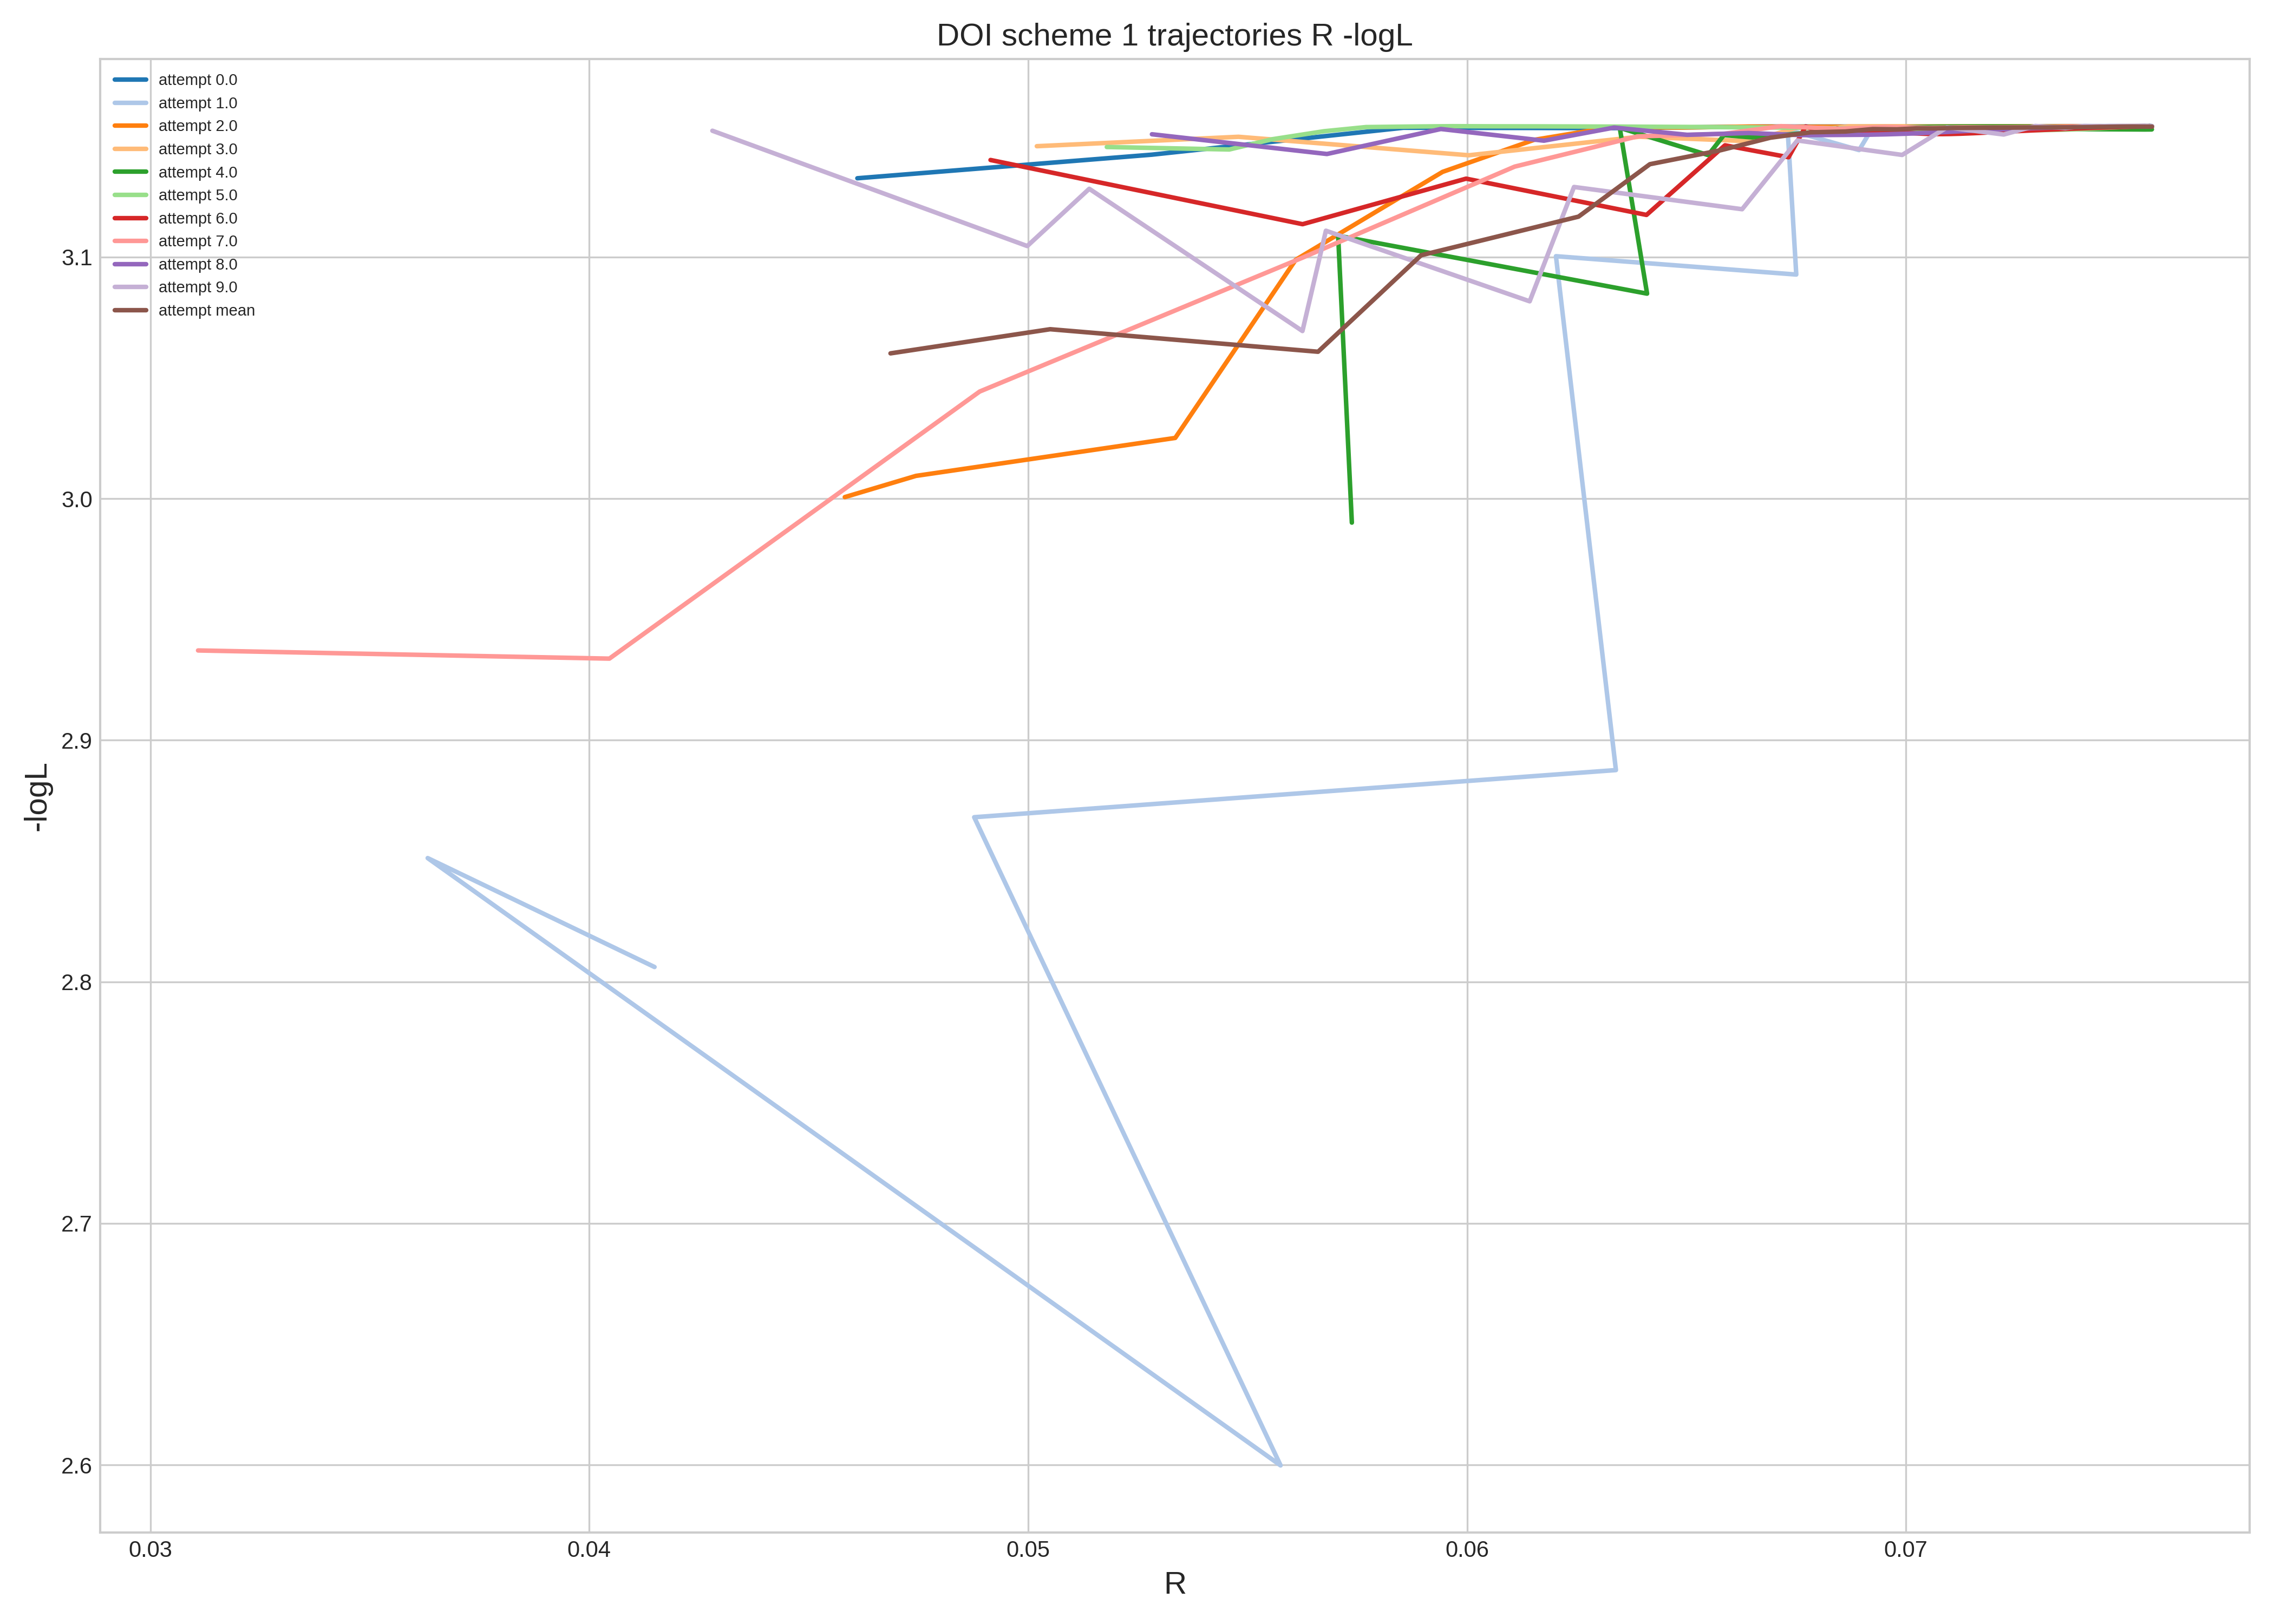
\includegraphics[width=\textwidth]{images/DOI scheme 1 trajectories R -logL.png}
        \captionsetup{font=tiny}
        \caption{2D $(R,-log(L))$ Trajectory Line Plot : DOI Method Type 1}
        \label{fig:corr_matrix_ts_qrt_data}
    \end{minipage}
\end{figure}
\level{3}{DOI Method : Type 2}
It is same as DOI Type 1, but uses OPI Type 2 in place of OPI Type 1 and here too to get better statistical result we ran the method multiple times with $N=1000$. This method has issues similar to DOI type 1 and OPI type 2, as it is not very smooth and the next update may not be nearby. But in $(R,-log(O))$ space, it is somewhat smooth, with little influence from regression to obtain $\beta$, which minimizes $L$.
\begin{figure}[H]
    \centering
    \begin{minipage}[t]{0.45\textwidth}
        \centering
        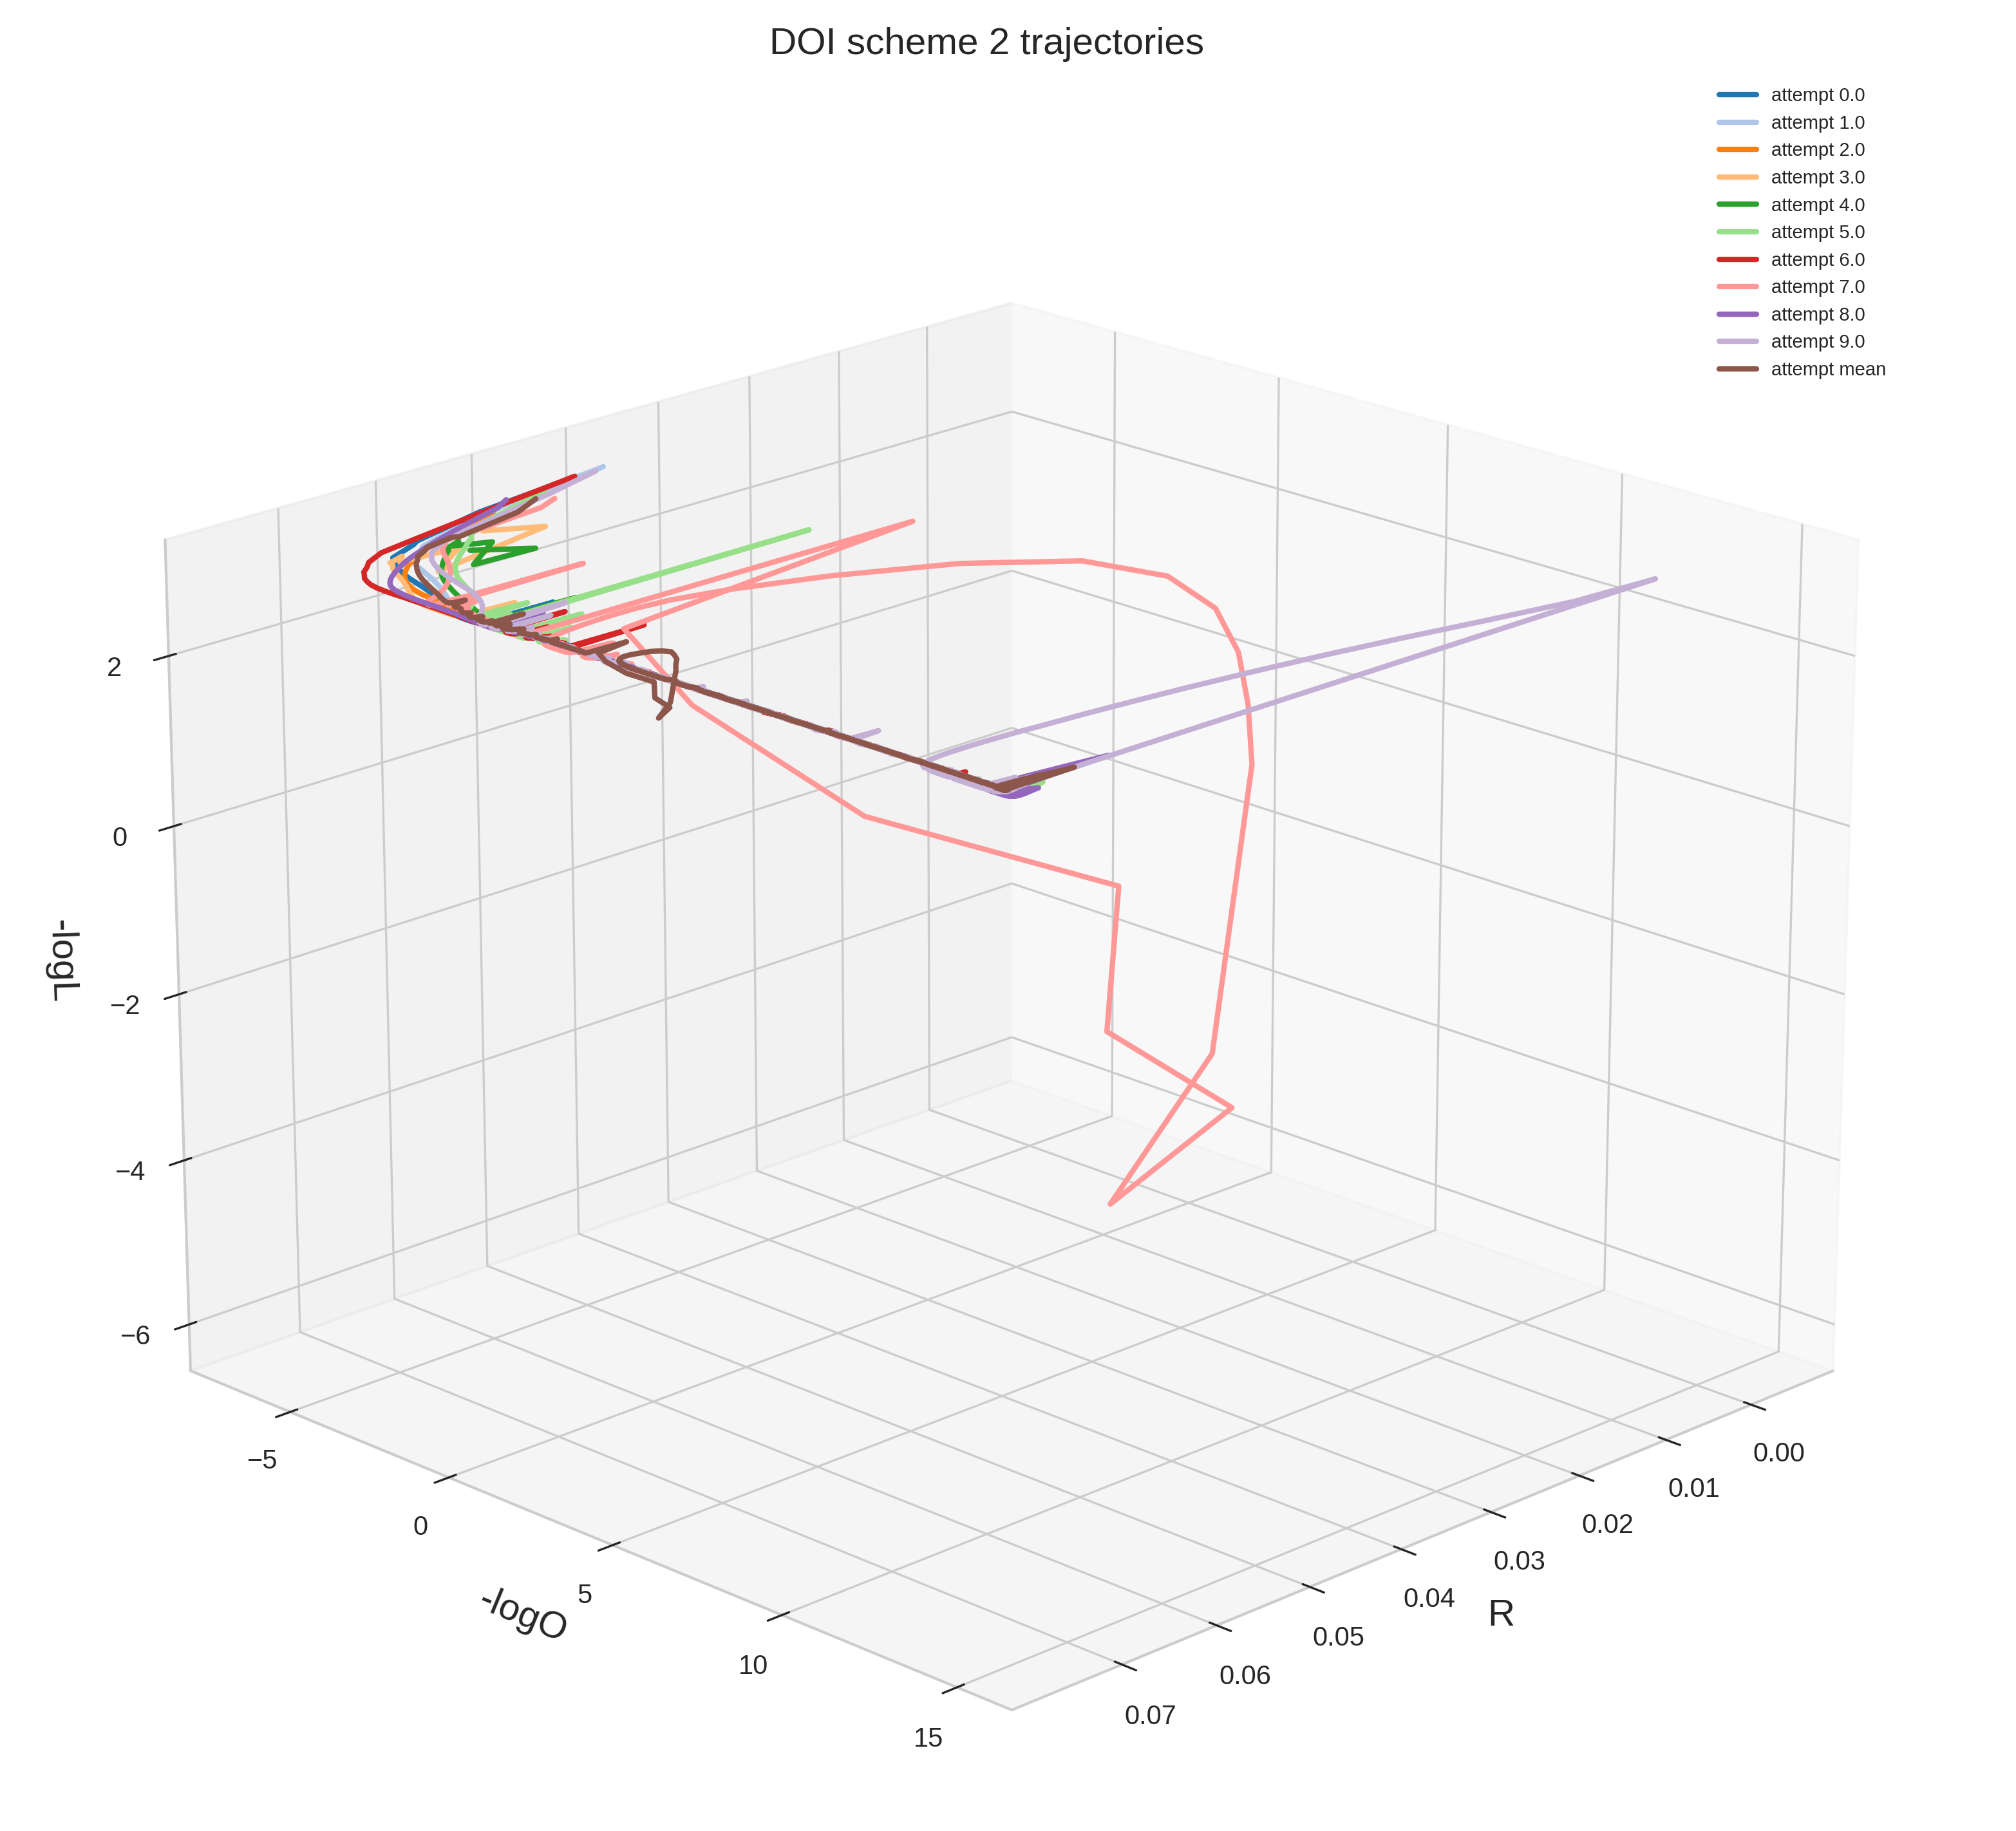
\includegraphics[width=\textwidth]{images/1-DOI scheme 2 mean trajectory.png}
        \captionsetup{font=tiny}
        \caption{3D Trajectory Line Plot : DOI Method Type 2}
        \label{fig:cumulative_returns}
    \end{minipage}%
    \begin{minipage}[t]{0.5511\textwidth}
        \centering
        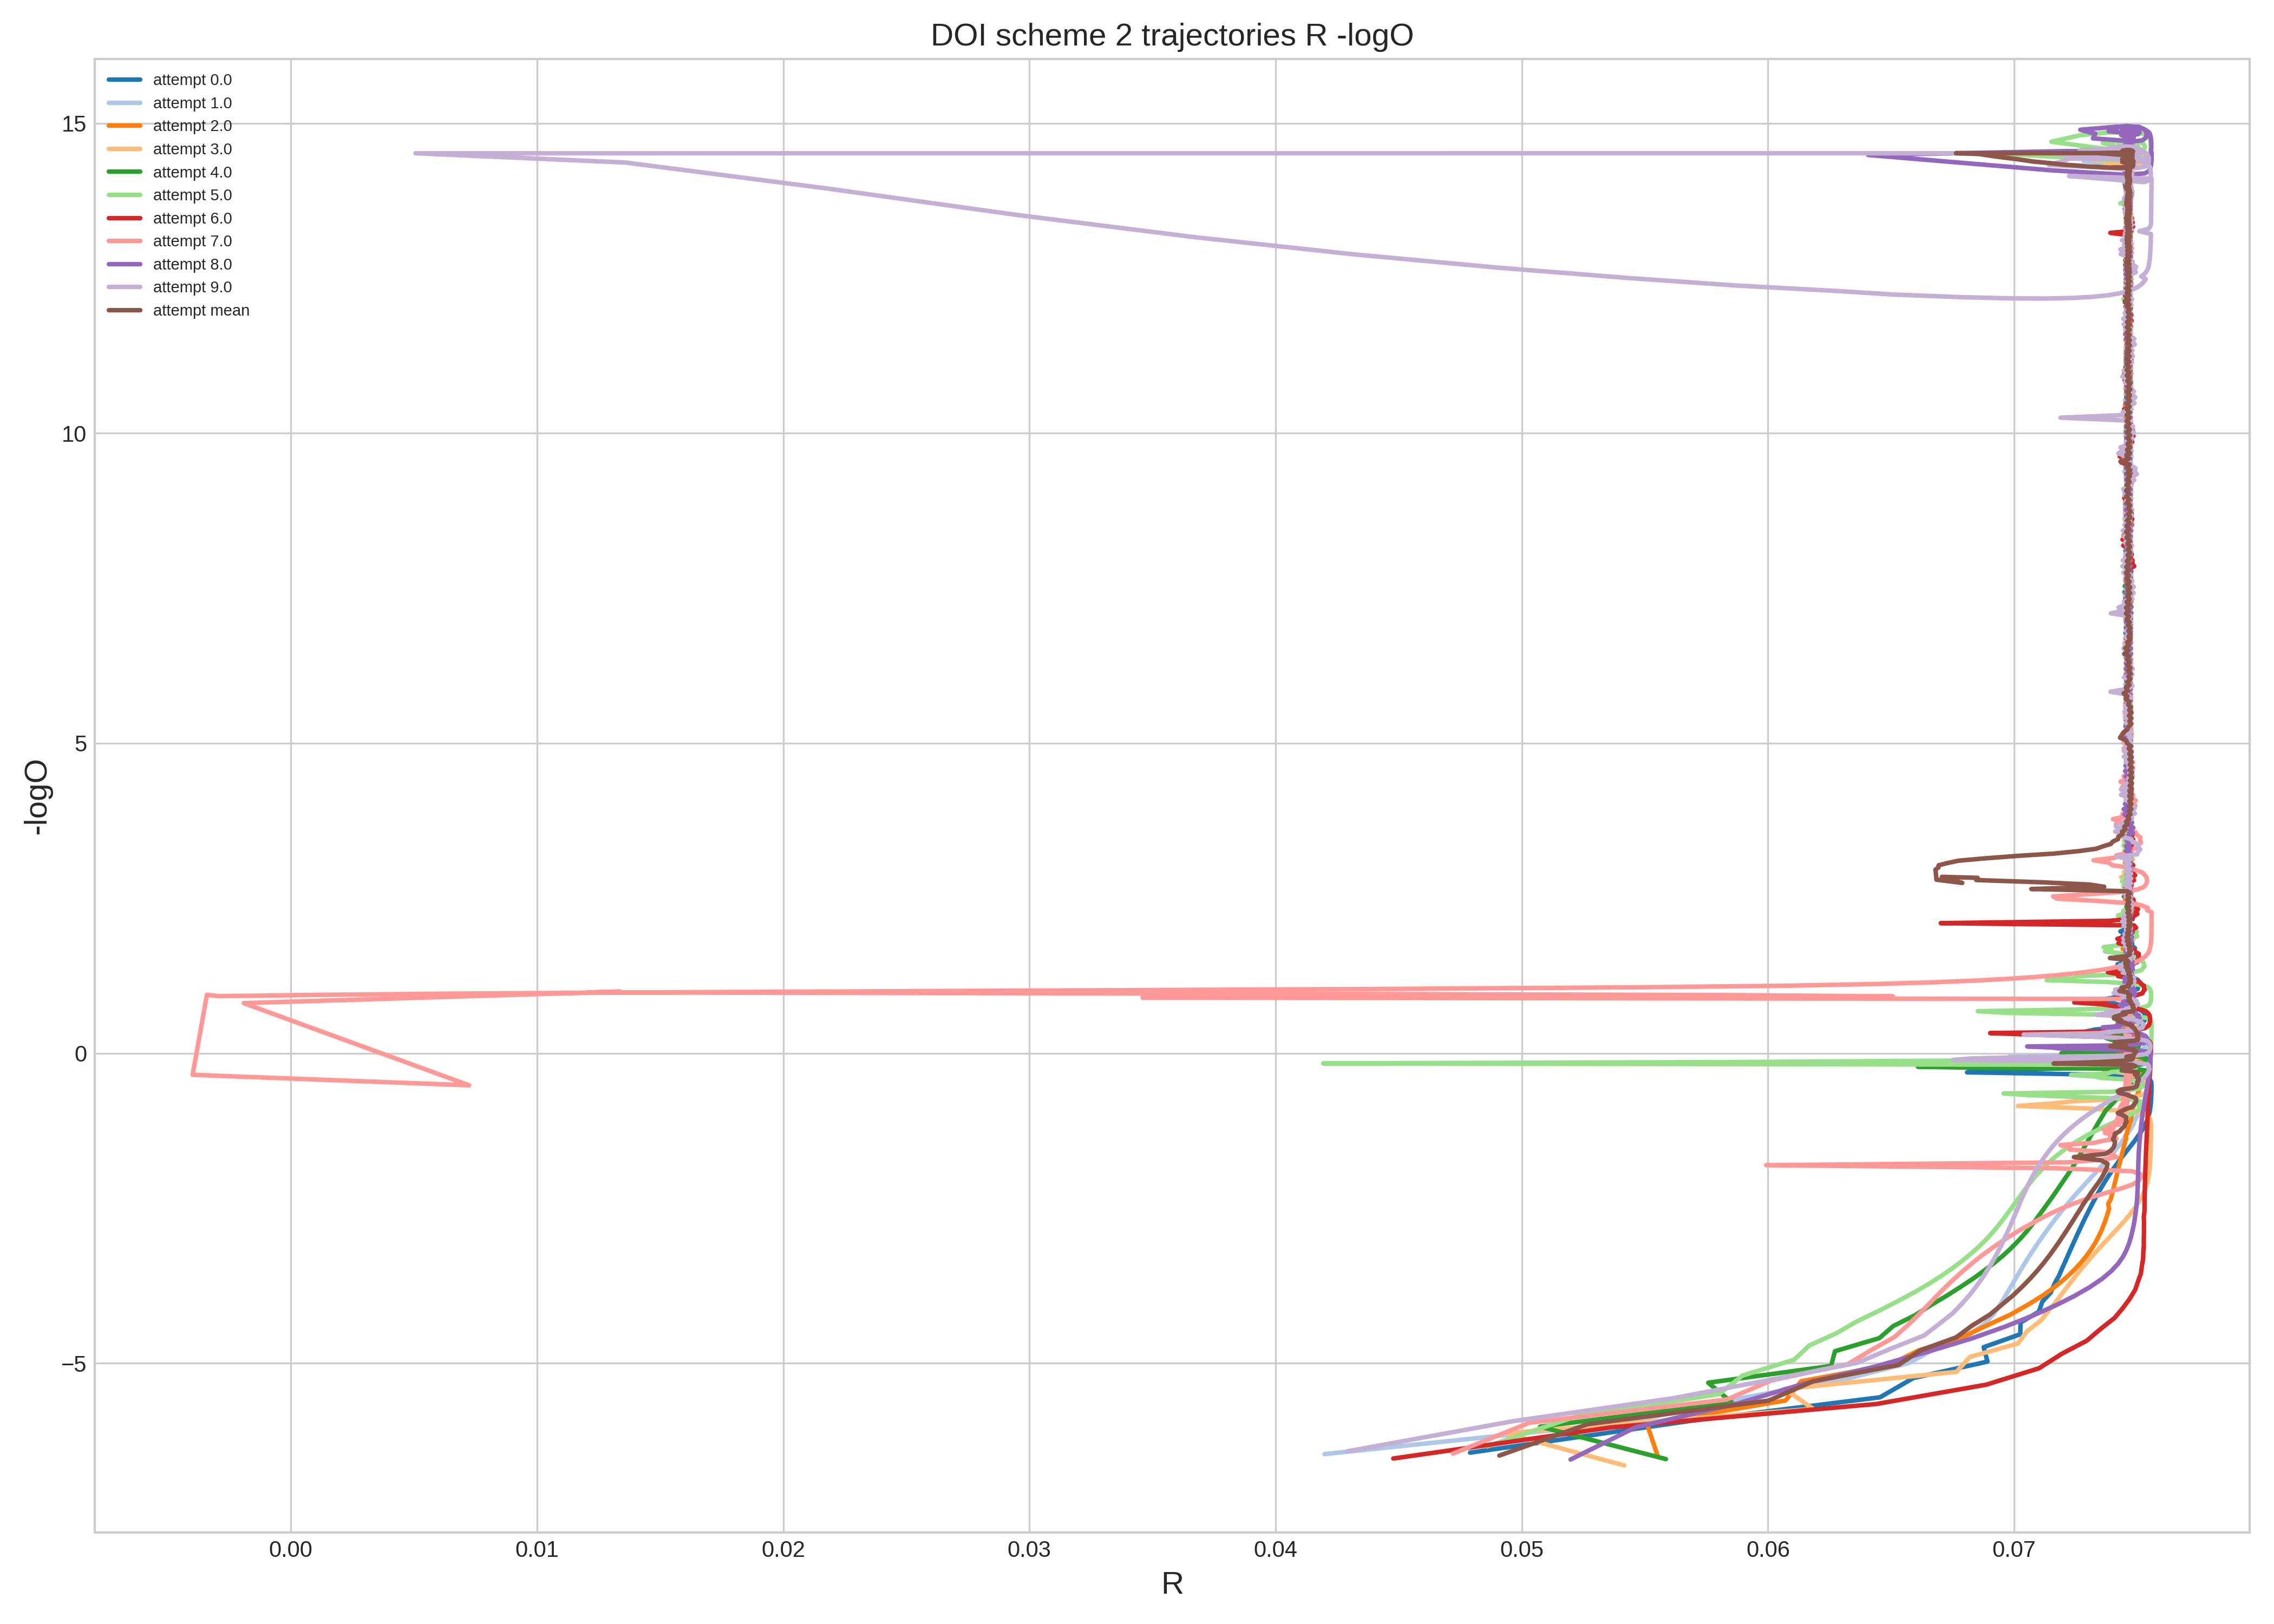
\includegraphics[width=\textwidth]{images/DOI scheme 2 trajectories R -logO.png}
        \captionsetup{font=tiny}
        \caption{2D $(R,-log(O))$ Trajectory Line Plot : DOI Method Type 2}
        \label{fig:corr_matrix_ts_qrt_data}
    \end{minipage}
\end{figure}

\level{3}{No Preference Method (NPM) : Type 1}
A learning rate of 0.01 is used for $A$ and $\beta$, with 1000 steps and NPM$_1[(0.01,0.01)]$. This method is observed to be very smooth, with all attempts converging to a point, and the update size decreasing over time.
\begin{figure}[H]
    \centering
    \begin{minipage}[t]{0.45\textwidth}
        \centering
        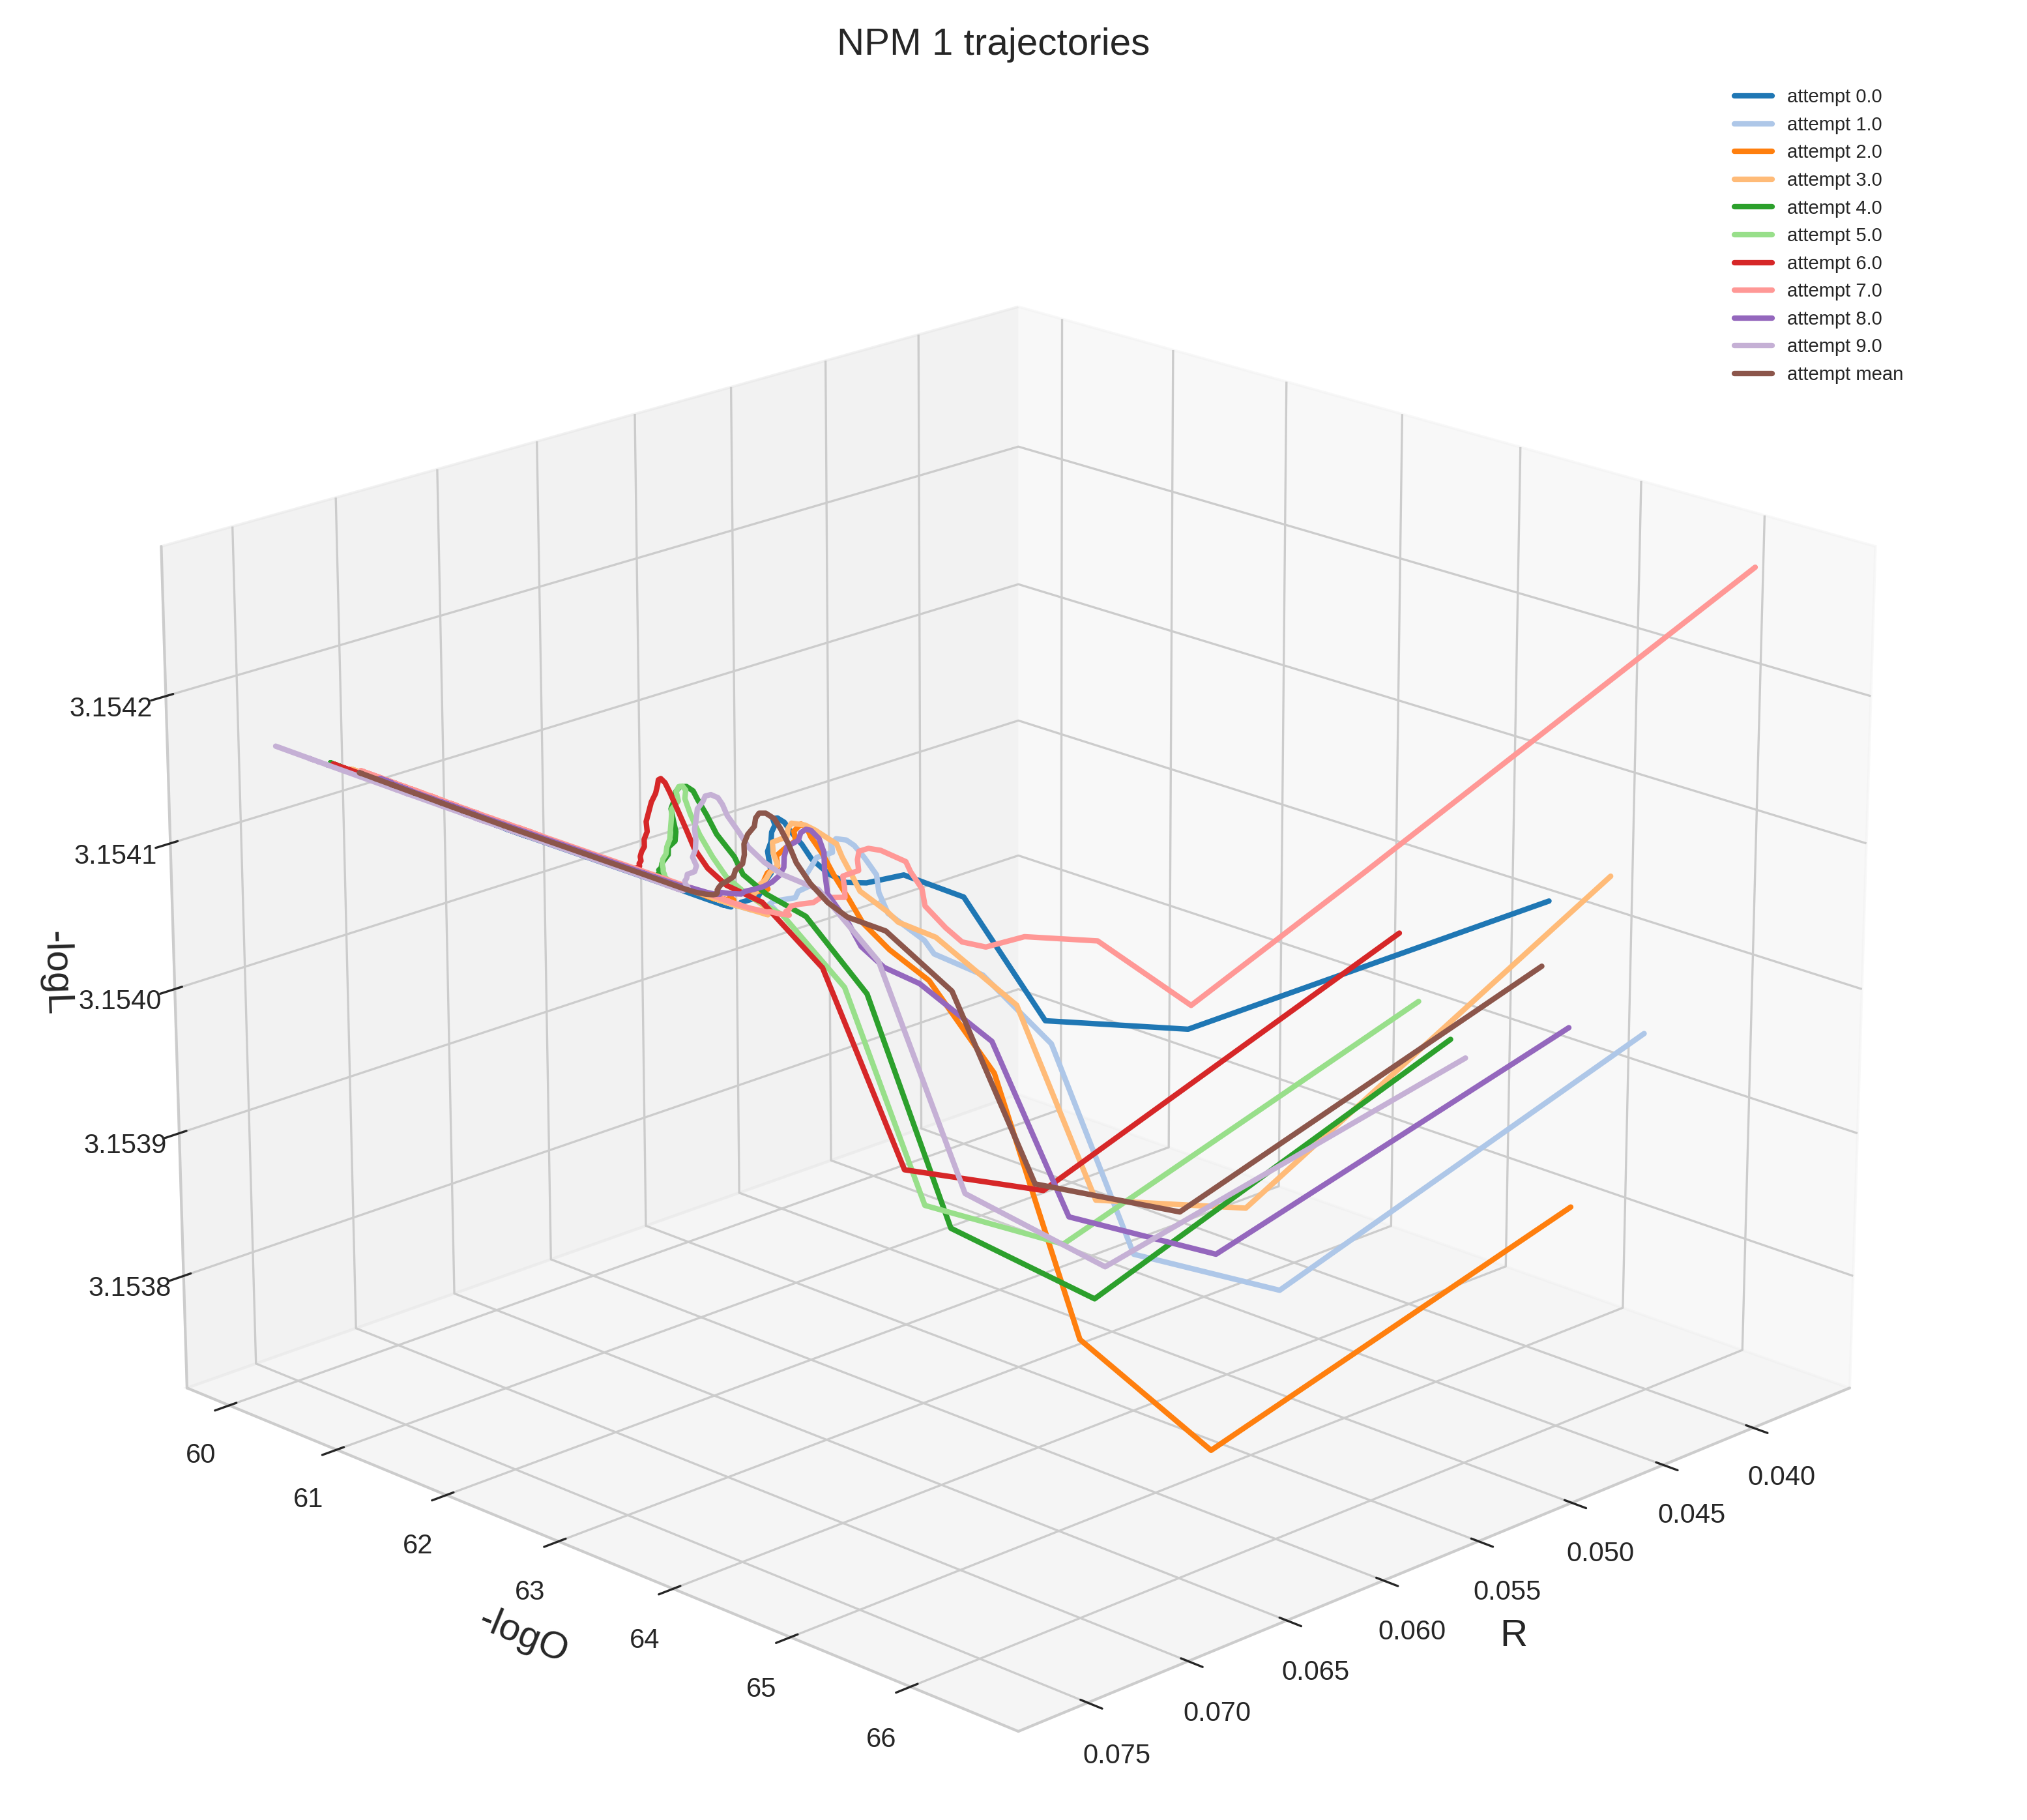
\includegraphics[width=\textwidth]{images/1-NPM 1 mean trajectory.png}
        \captionsetup{font=tiny}
        \caption{3D Trajectory Line Plot : NPM Type 1}
        \label{fig:cumulative_returns}
    \end{minipage}%
    \begin{minipage}[t]{0.5511\textwidth}
        \centering
        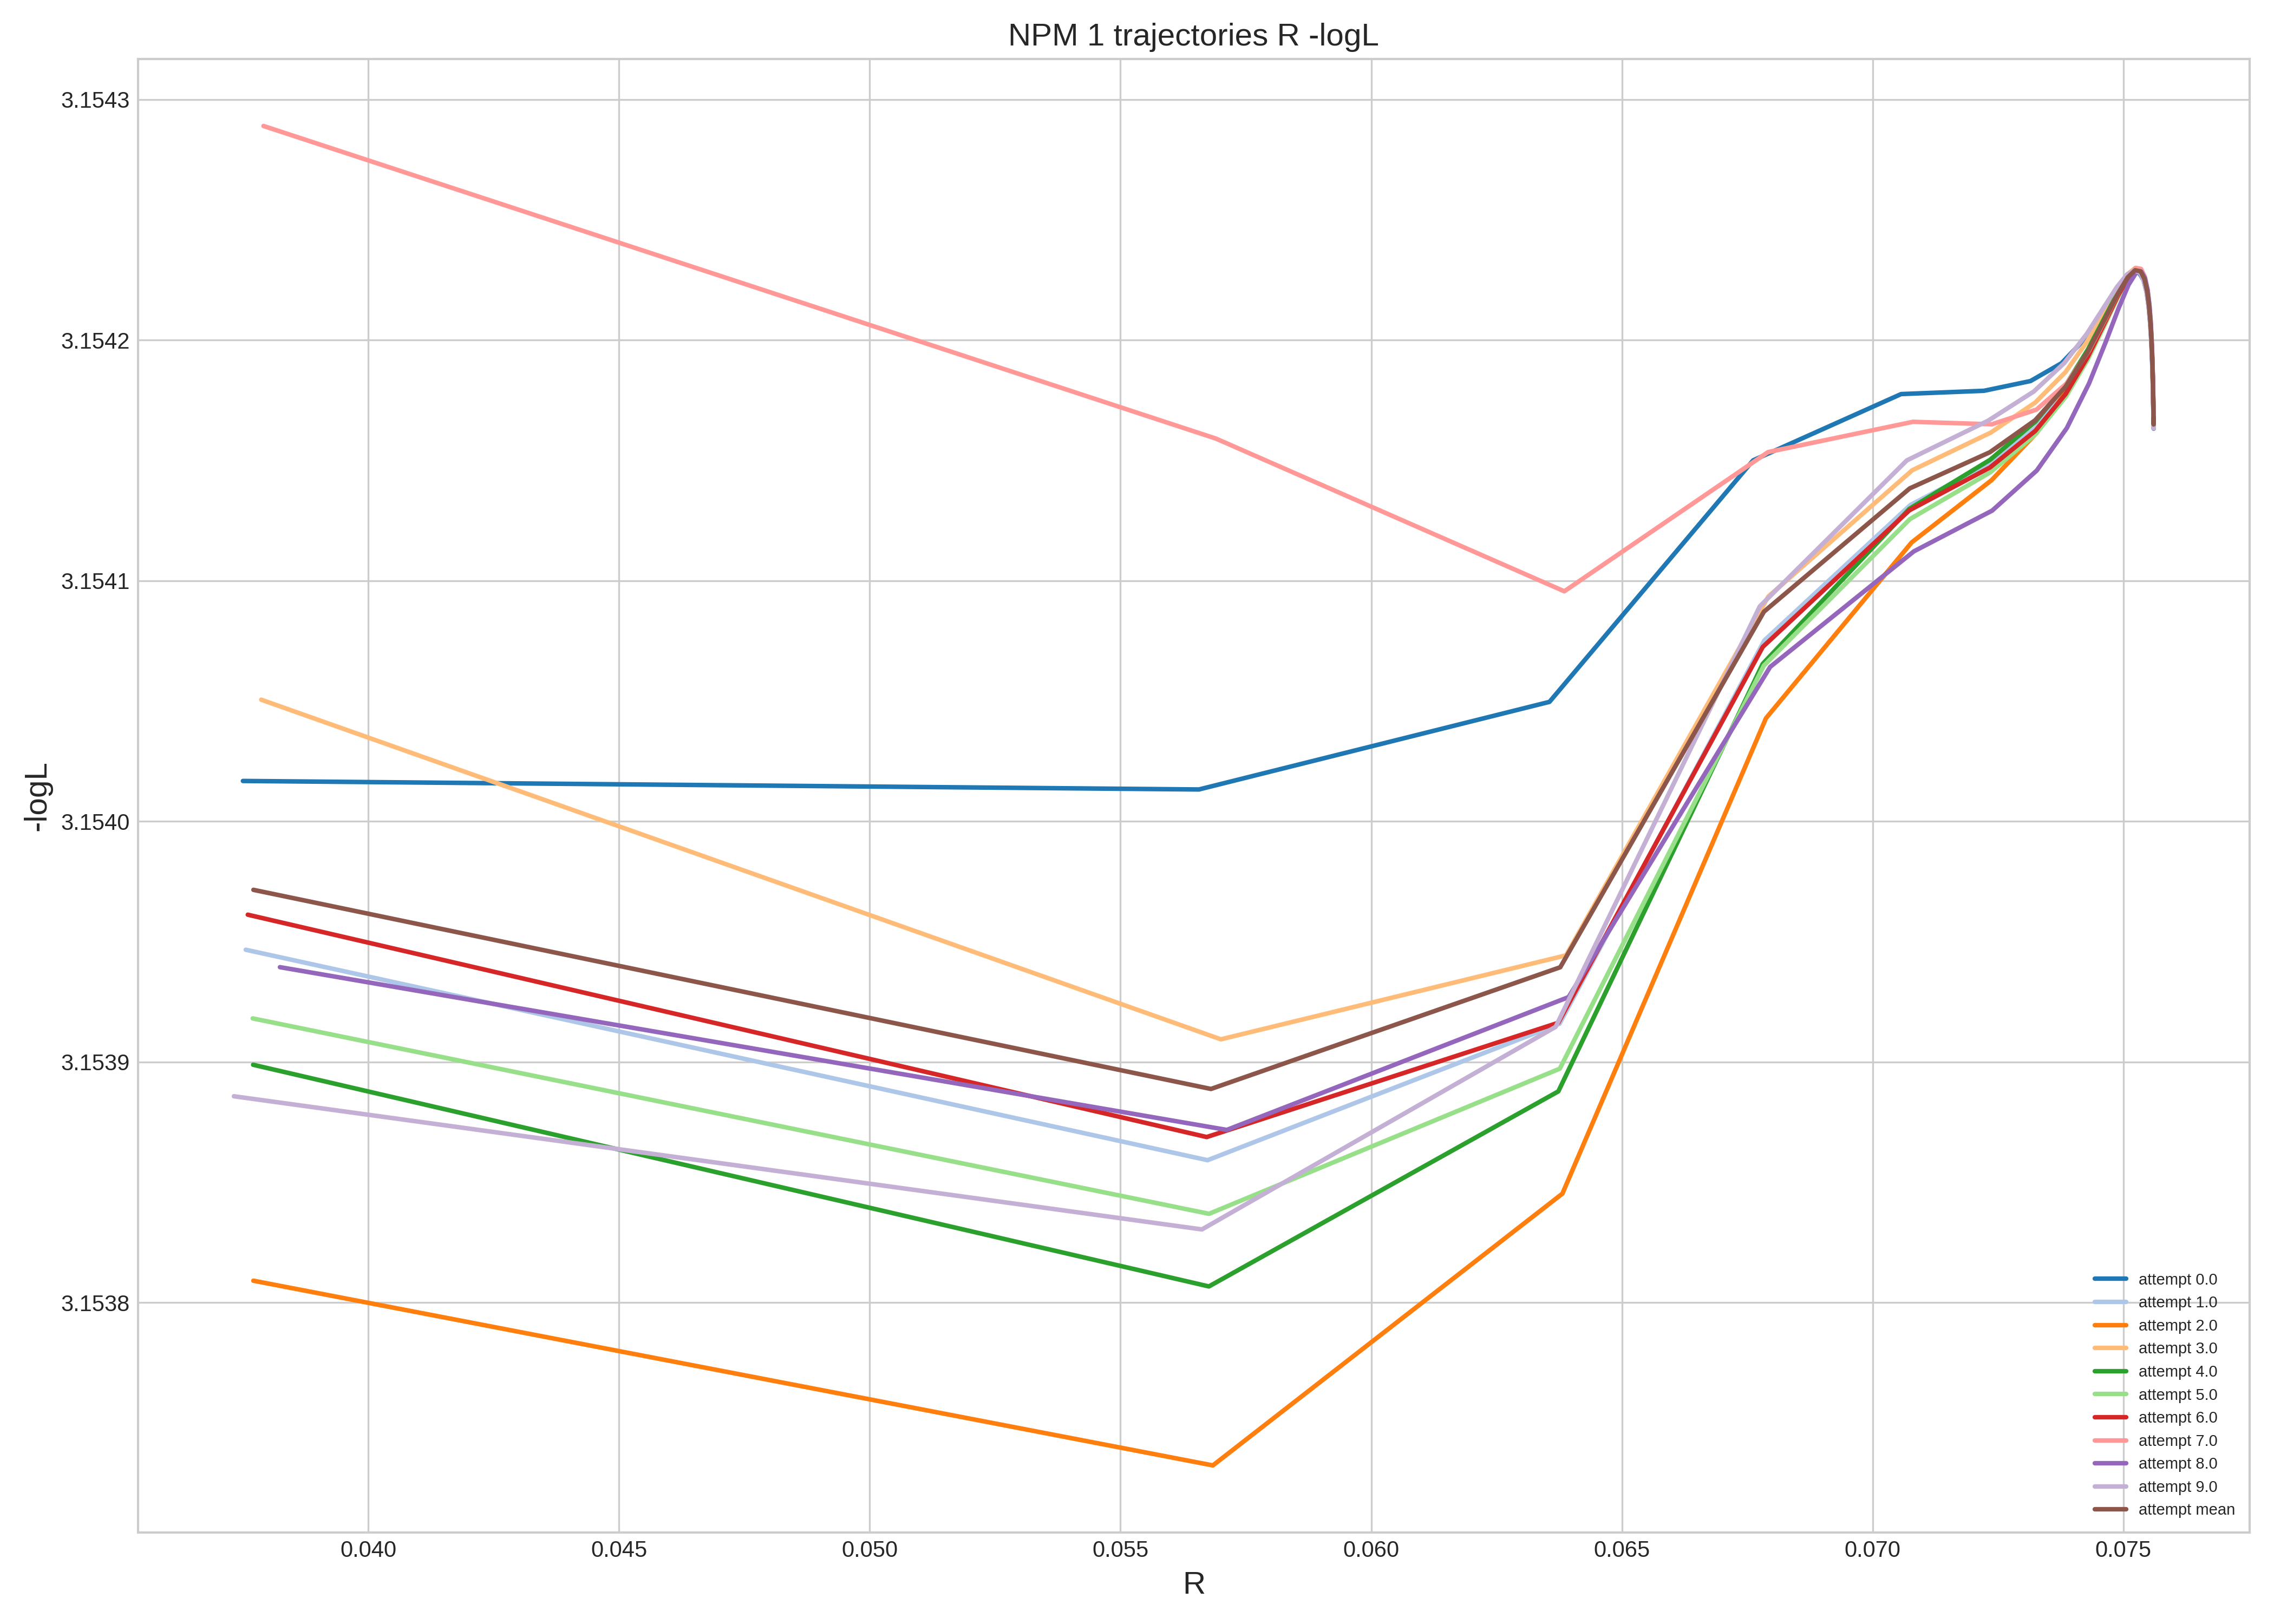
\includegraphics[width=\textwidth]{images/NPM 1 trajectories R -logL.png}
        \captionsetup{font=tiny}
        \caption{2D $(R,-log(L))$ Trajectory Line Plot : NPM Type 1}
        \label{fig:corr_matrix_ts_qrt_data}
    \end{minipage}
\end{figure} 
\level{3}{No Preference Method (NPM) : Type 2} 
The method uses a learning rate of 0.01 for both $A$ and $\beta$, with 1000 steps and NPM$_2[(0.01,0.01)]$. However, it doesn't utilize the orthogonal property and Cayley transform to update $A$. As seen in the figures, the method is smooth and converges with decreasing update size. However, there is some variation in the convergence point.
\begin{figure}[H]
    \centering
    \begin{minipage}[t]{0.45\textwidth}
        \centering
        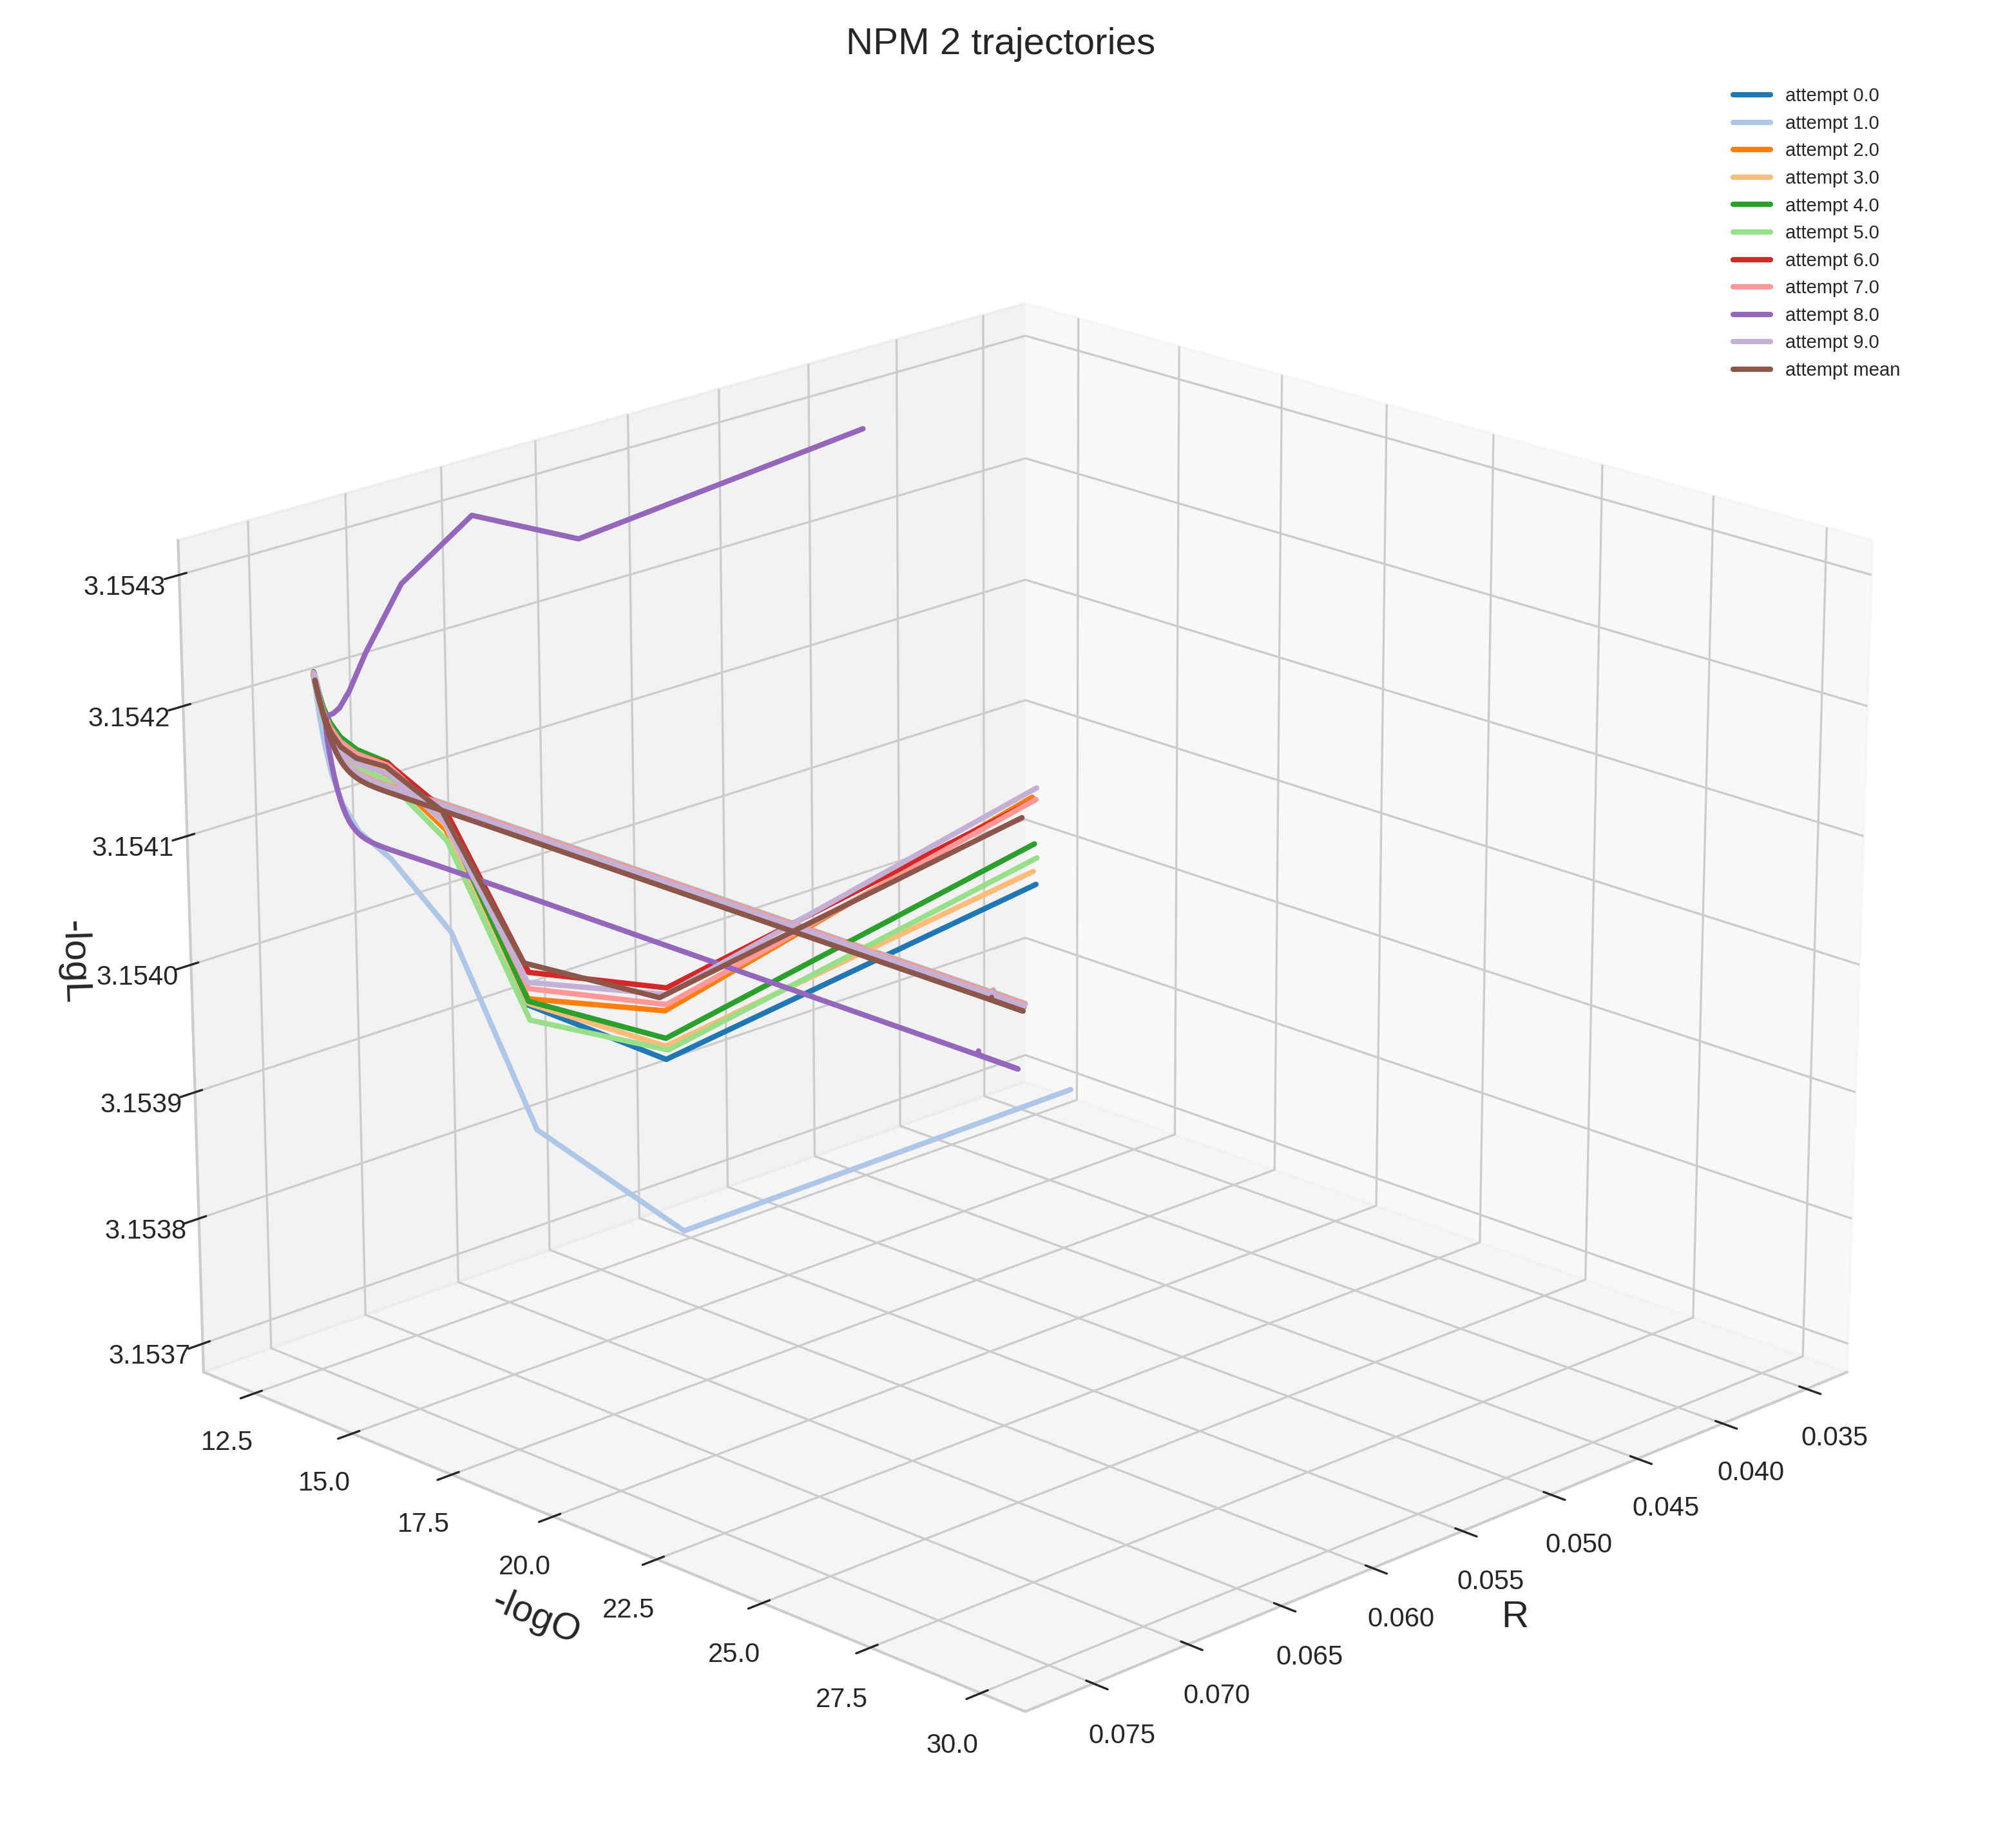
\includegraphics[width=\textwidth]{images/1-NPM 2 mean trajectory.png}
        \captionsetup{font=tiny}
        \caption{3D Trajectory Line Plot : NPM Type 2}
        \label{fig:cumulative_returns}
    \end{minipage}%
    \begin{minipage}[t]{0.5511\textwidth}
        \centering
        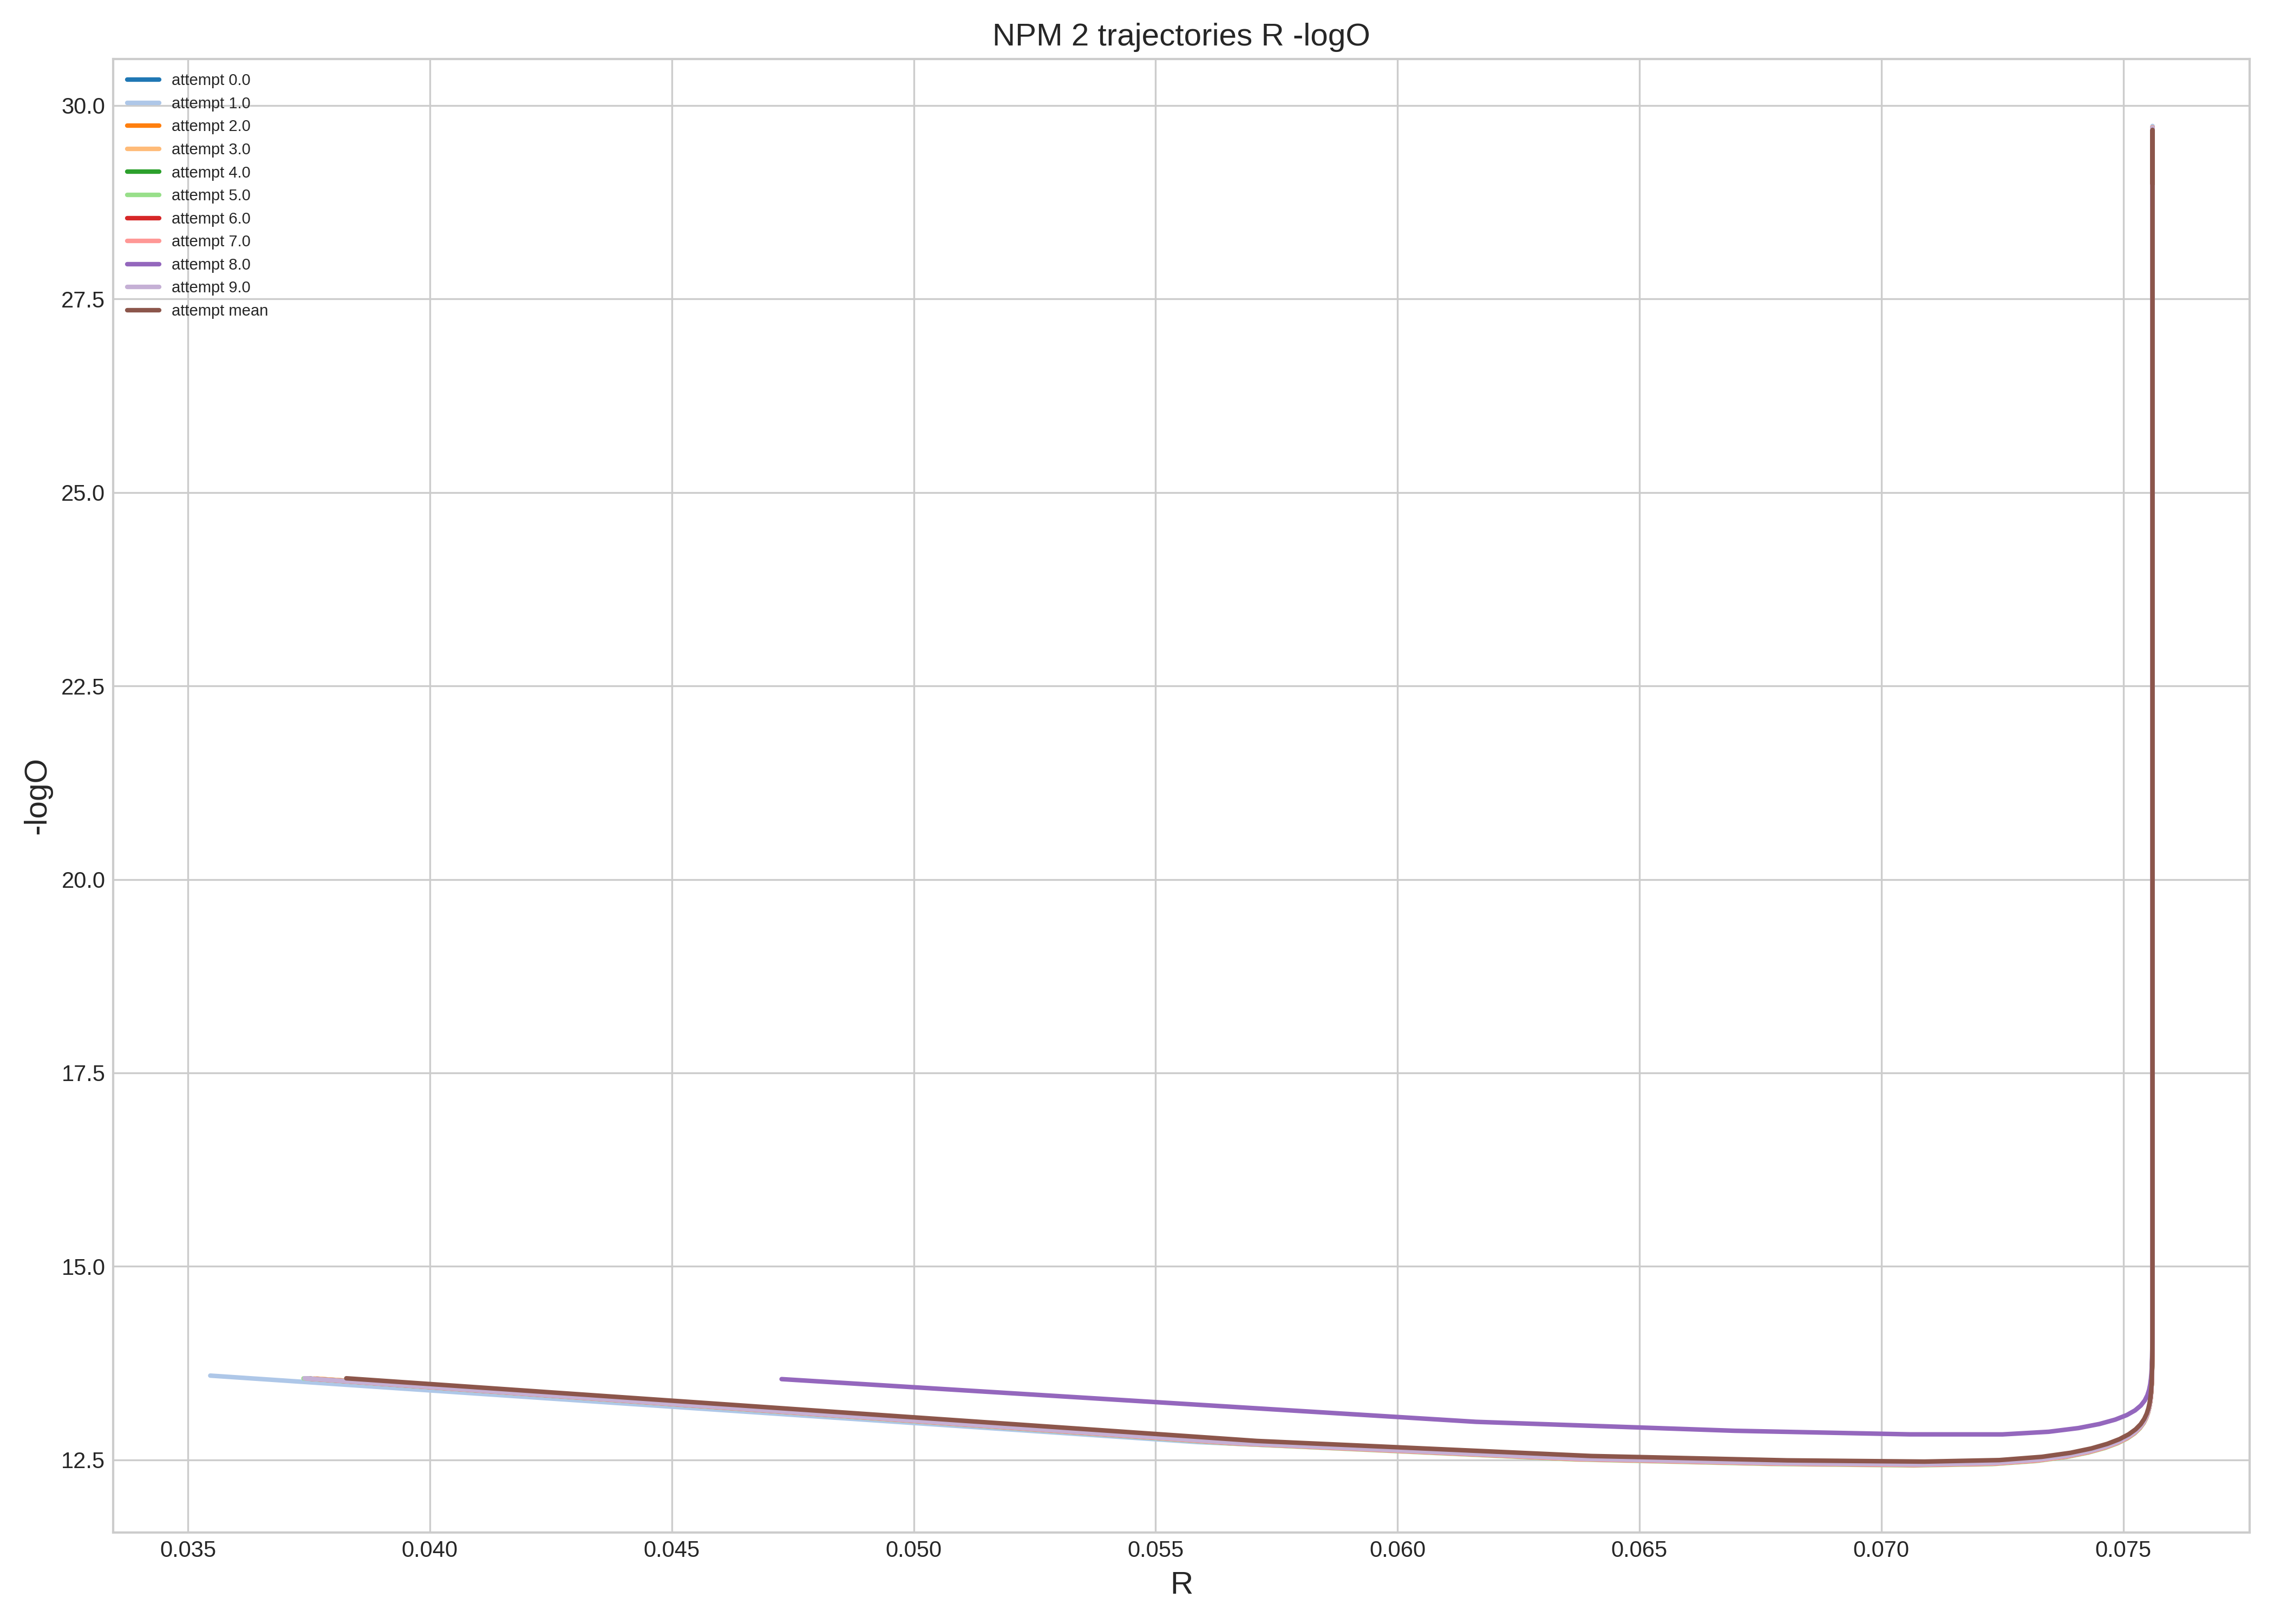
\includegraphics[width=\textwidth]{images/NPM 2 trajectories R -logO.png}
        \captionsetup{font=tiny}
        \caption{2D $(R,-log(O))$ Trajectory Line Plot :NPM Type 2}
        \label{fig:corr_matrix_ts_qrt_data}
    \end{minipage}
\end{figure} 
\level{3}{NSGA-II}
\textbf{Type 1} : In this NSGA-II type we dont use regression for updating $\beta$ and the parameters of this are 
NSGA-II$(100,500,1,0.2,\mathcal{C}[\text{No Regression},0.01],\mathcal{M}[0.01])$, that is with population size of 500 and number of generations 100. We observe that, except for the first generation, all the points lie on a non-dominant front and the performance appears to be improving steadily with each generation. \newline \textbf{Type 2}: This uses regression for updating $\beta$. We can see that there are multiple non-dominant fronts and as we reach convergence we have only 1 non-dominant front.
\begin{figure}[H]
  \centering
  \begin{minipage}[b]{0.22\textwidth}
  \begin{figure}[H]
      \centering
      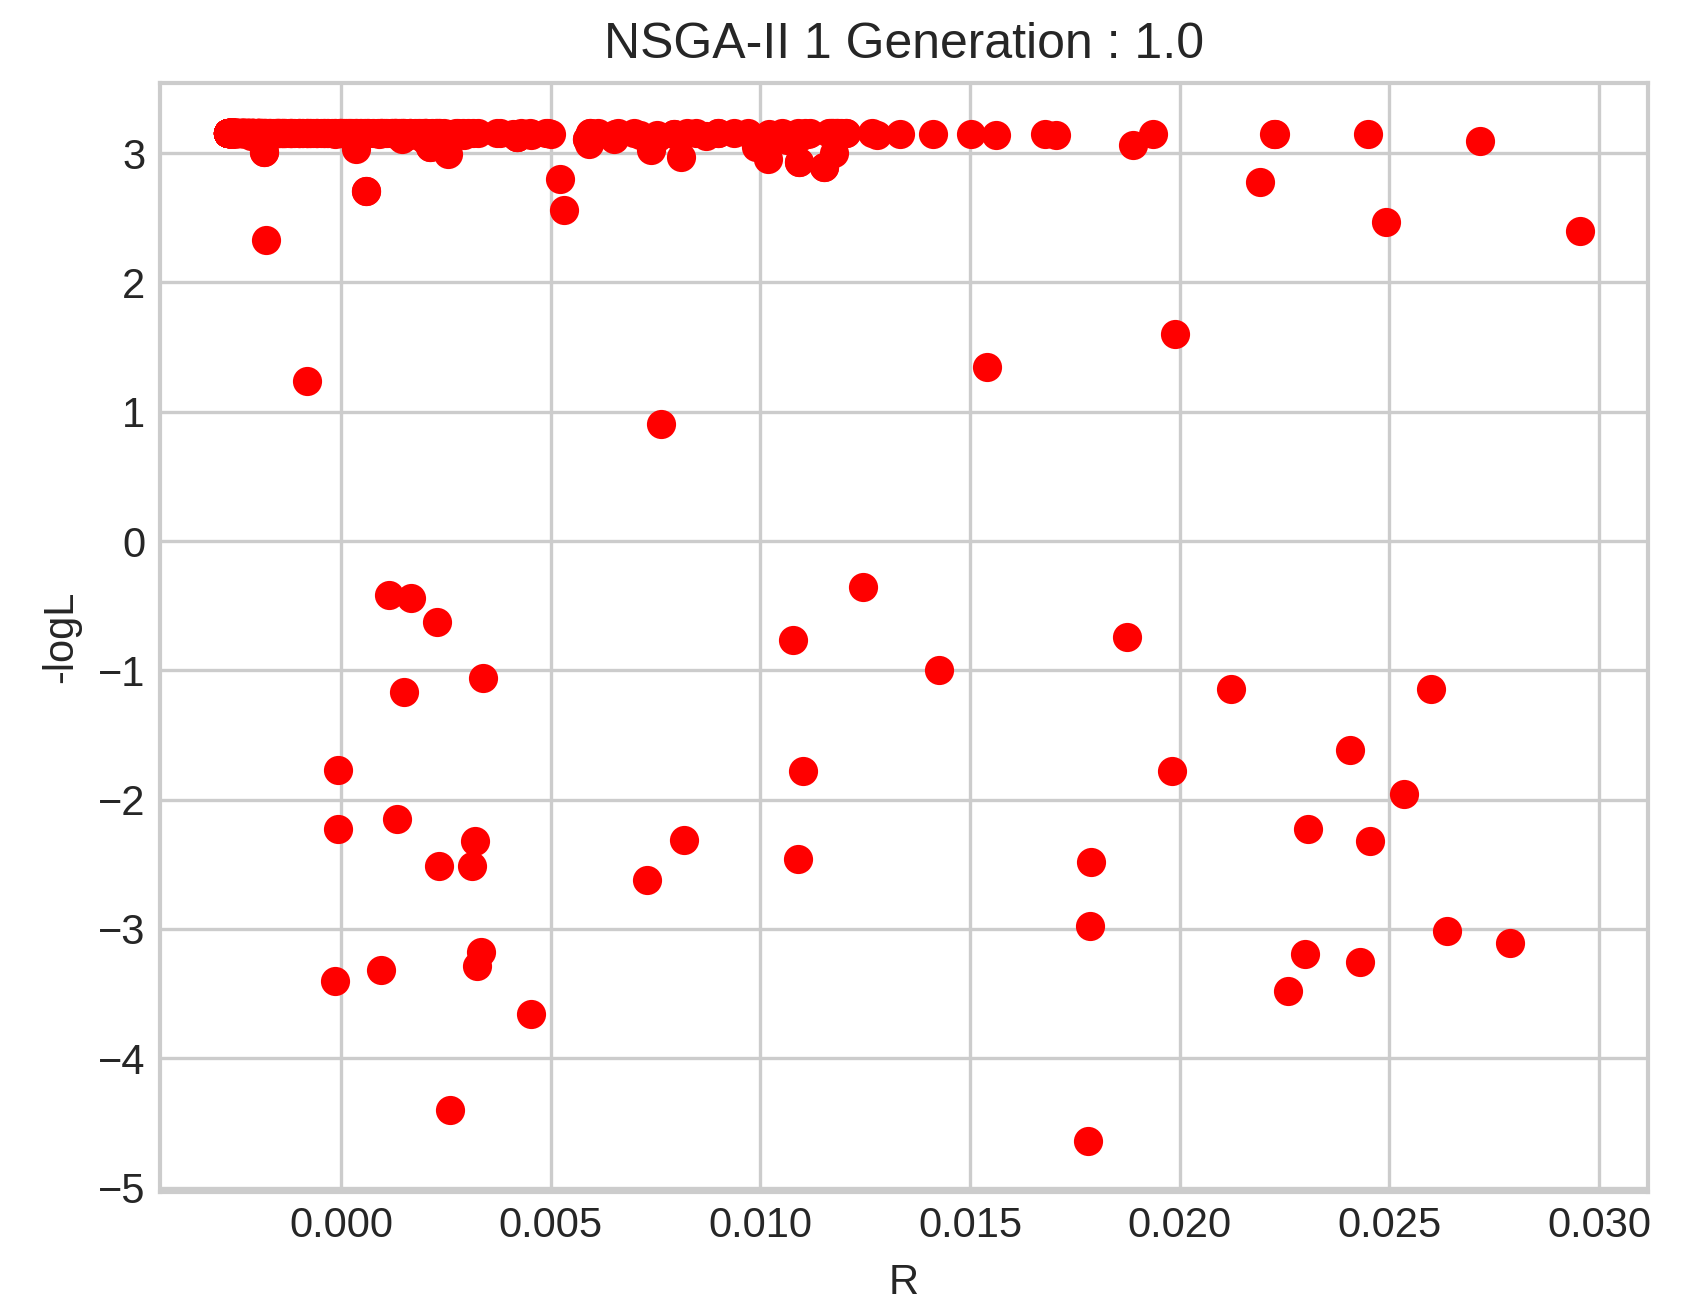
\includegraphics[width=\textwidth]{images/1-NSGA-II 1 Generation _ 1.0-R - logL-point.png}
  \end{figure}
  \end{minipage}
  \hspace{0.0cm}
  \begin{minipage}[b]{0.22\textwidth}
  \begin{figure}[H]
      \centering
      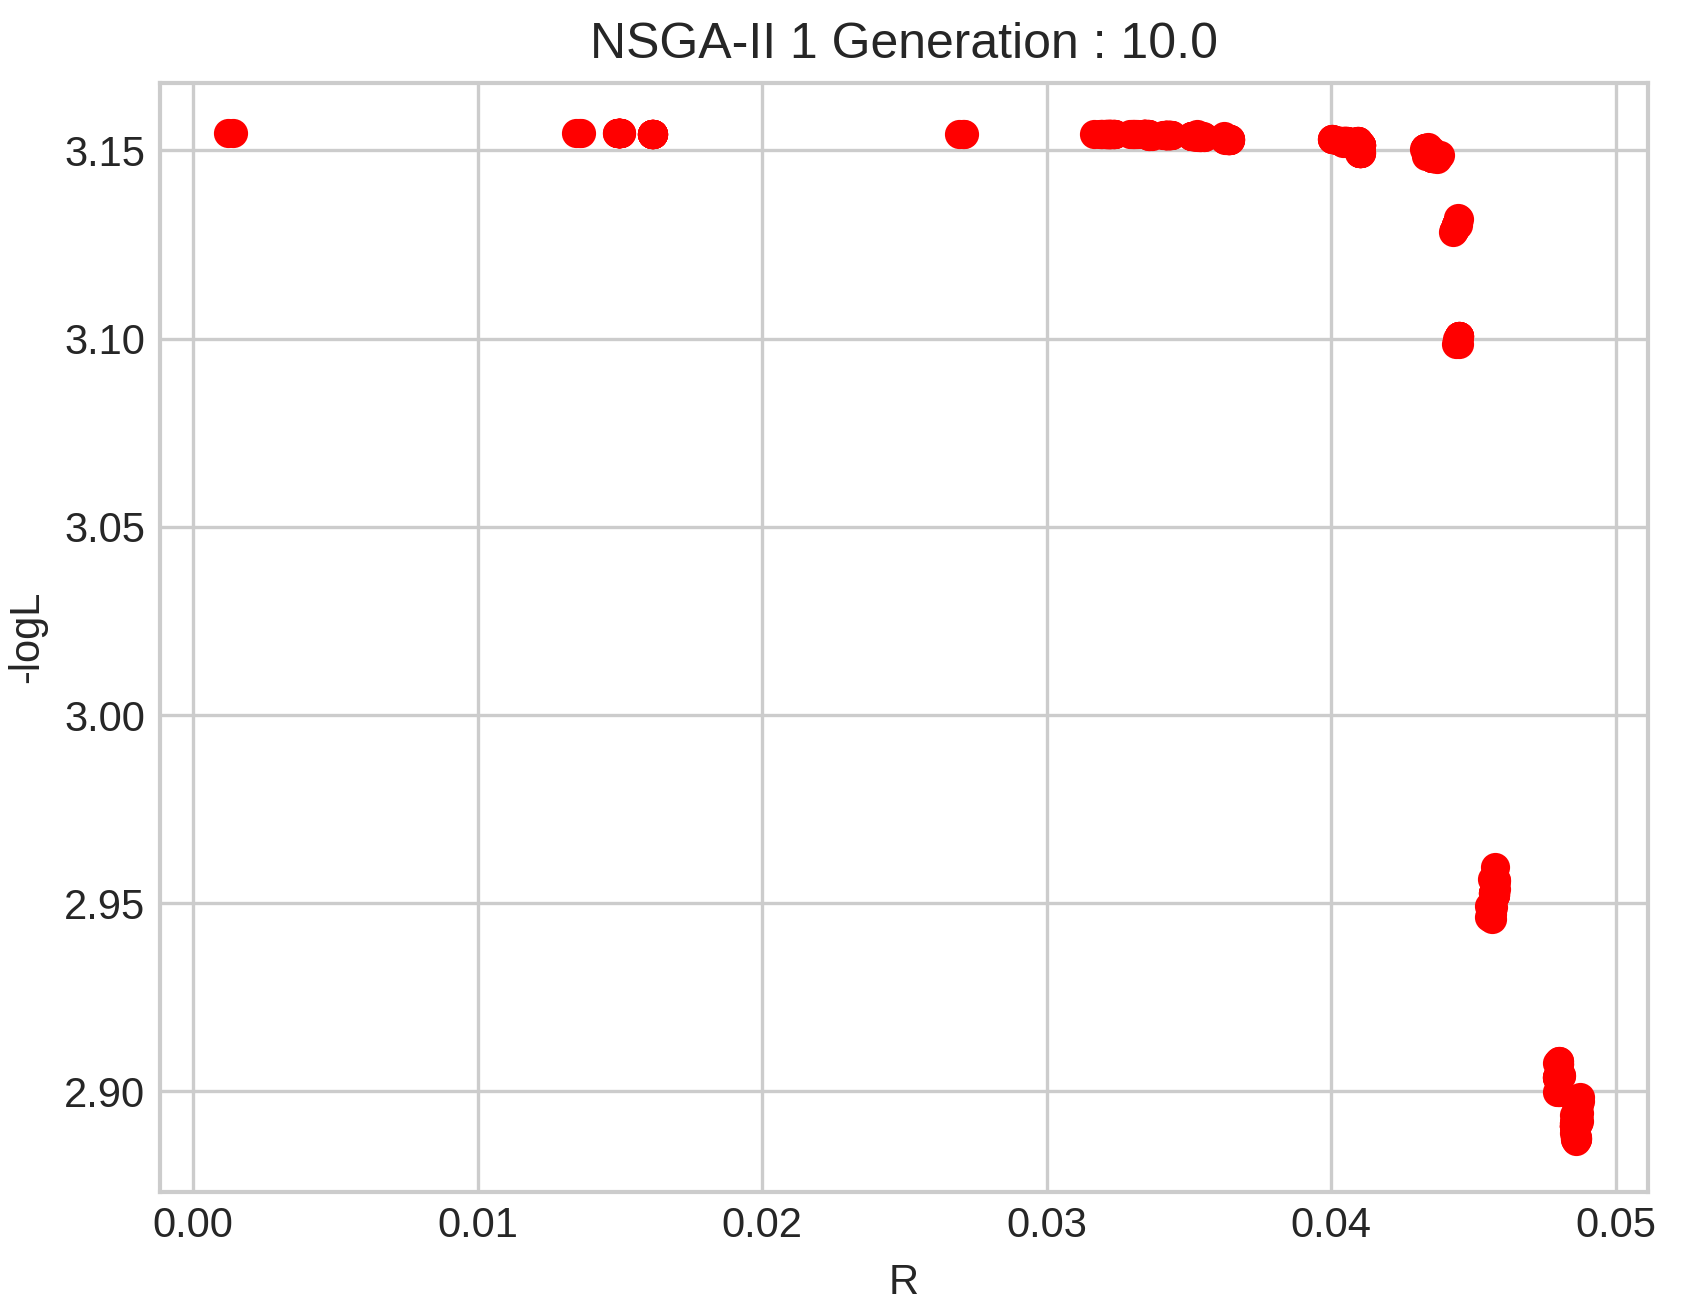
\includegraphics[width=\textwidth]{images/1-NSGA-II 1 Generation _ 10.0-R - logL-point.png}
  \end{figure}
  \end{minipage}
  \hspace{0.0cm}
  \begin{minipage}[b]{0.22\textwidth}
  \begin{figure}[H]
      \centering
      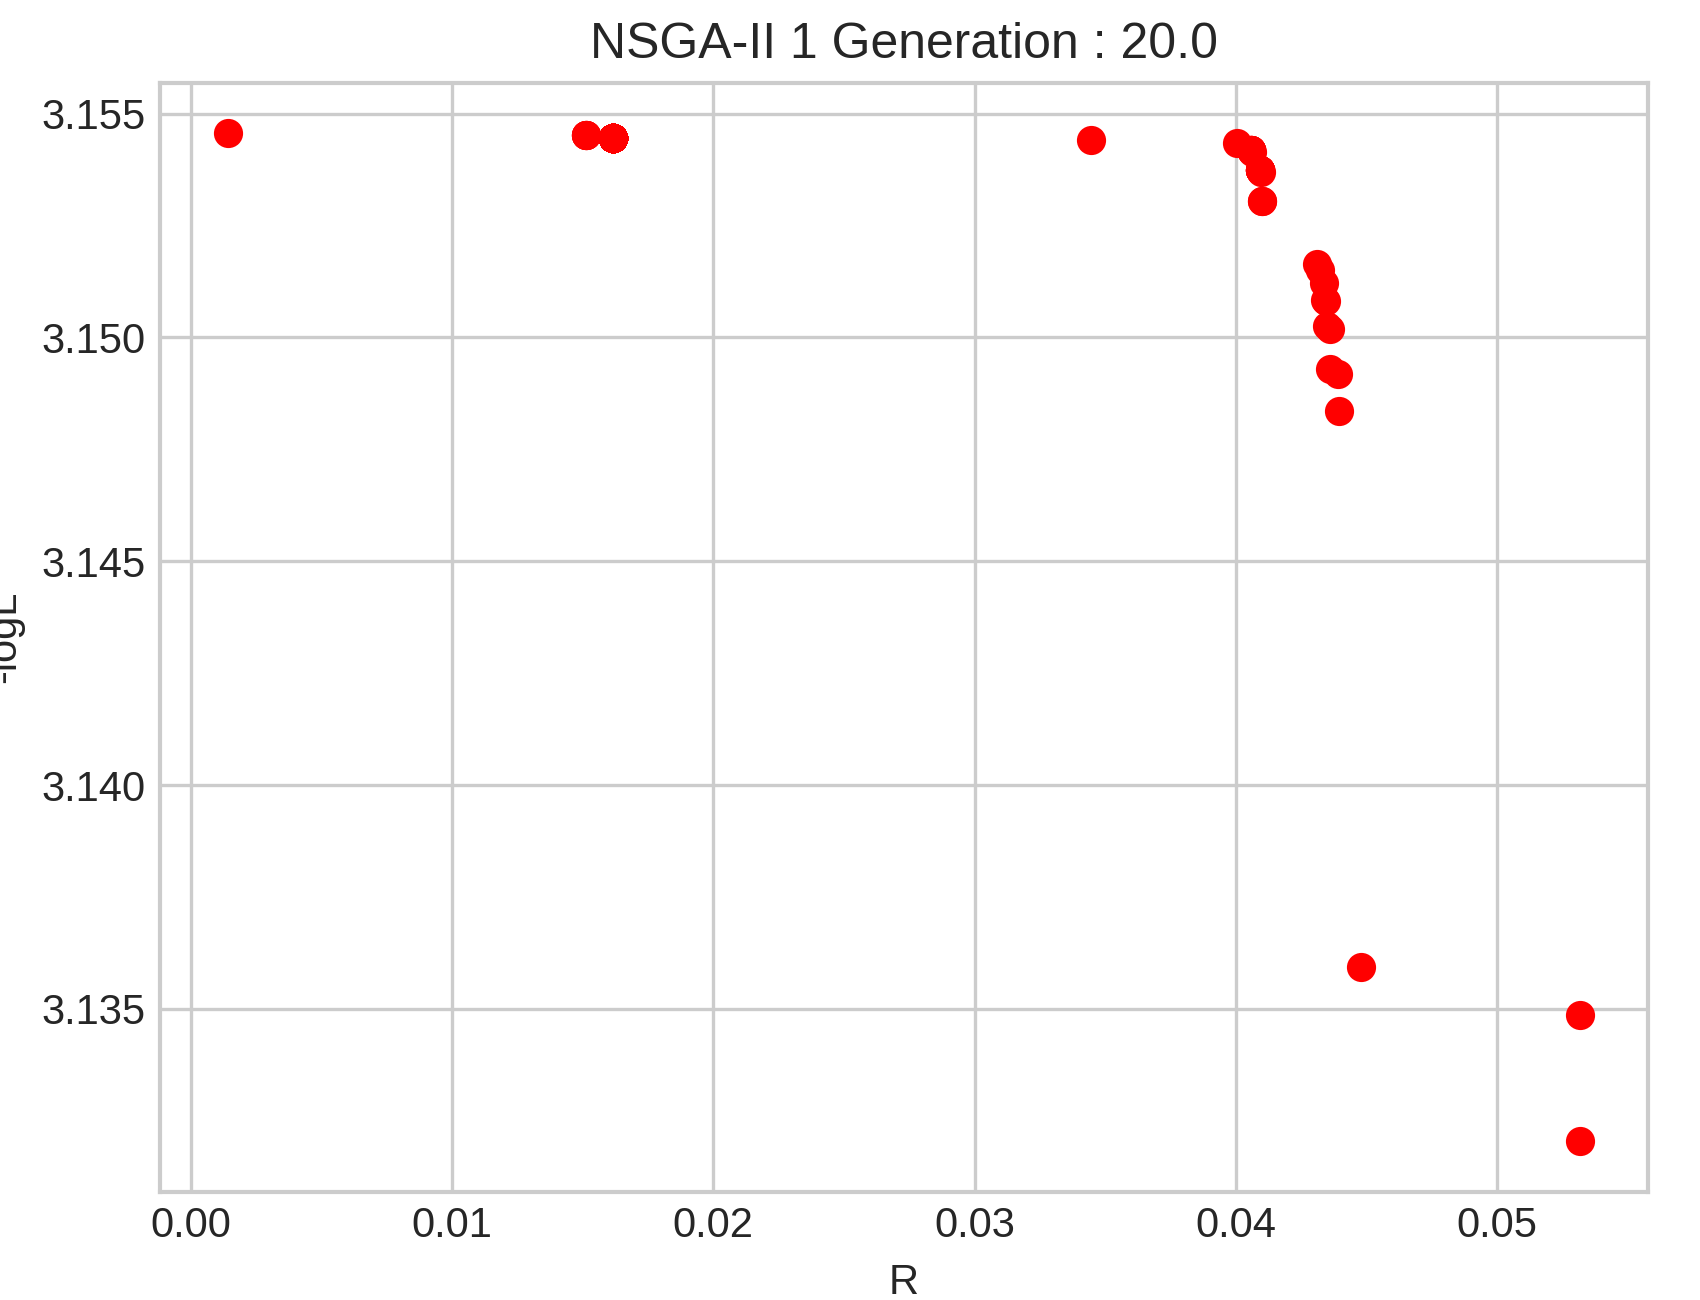
\includegraphics[width=\textwidth]{images/1-NSGA-II 1 Generation _ 20.0-R - logL-point.png}
  \end{figure}
  \end{minipage}
  \hspace{0.0cm}
  \begin{minipage}[b]{0.22\textwidth}
  \begin{figure}[H]
      \centering
      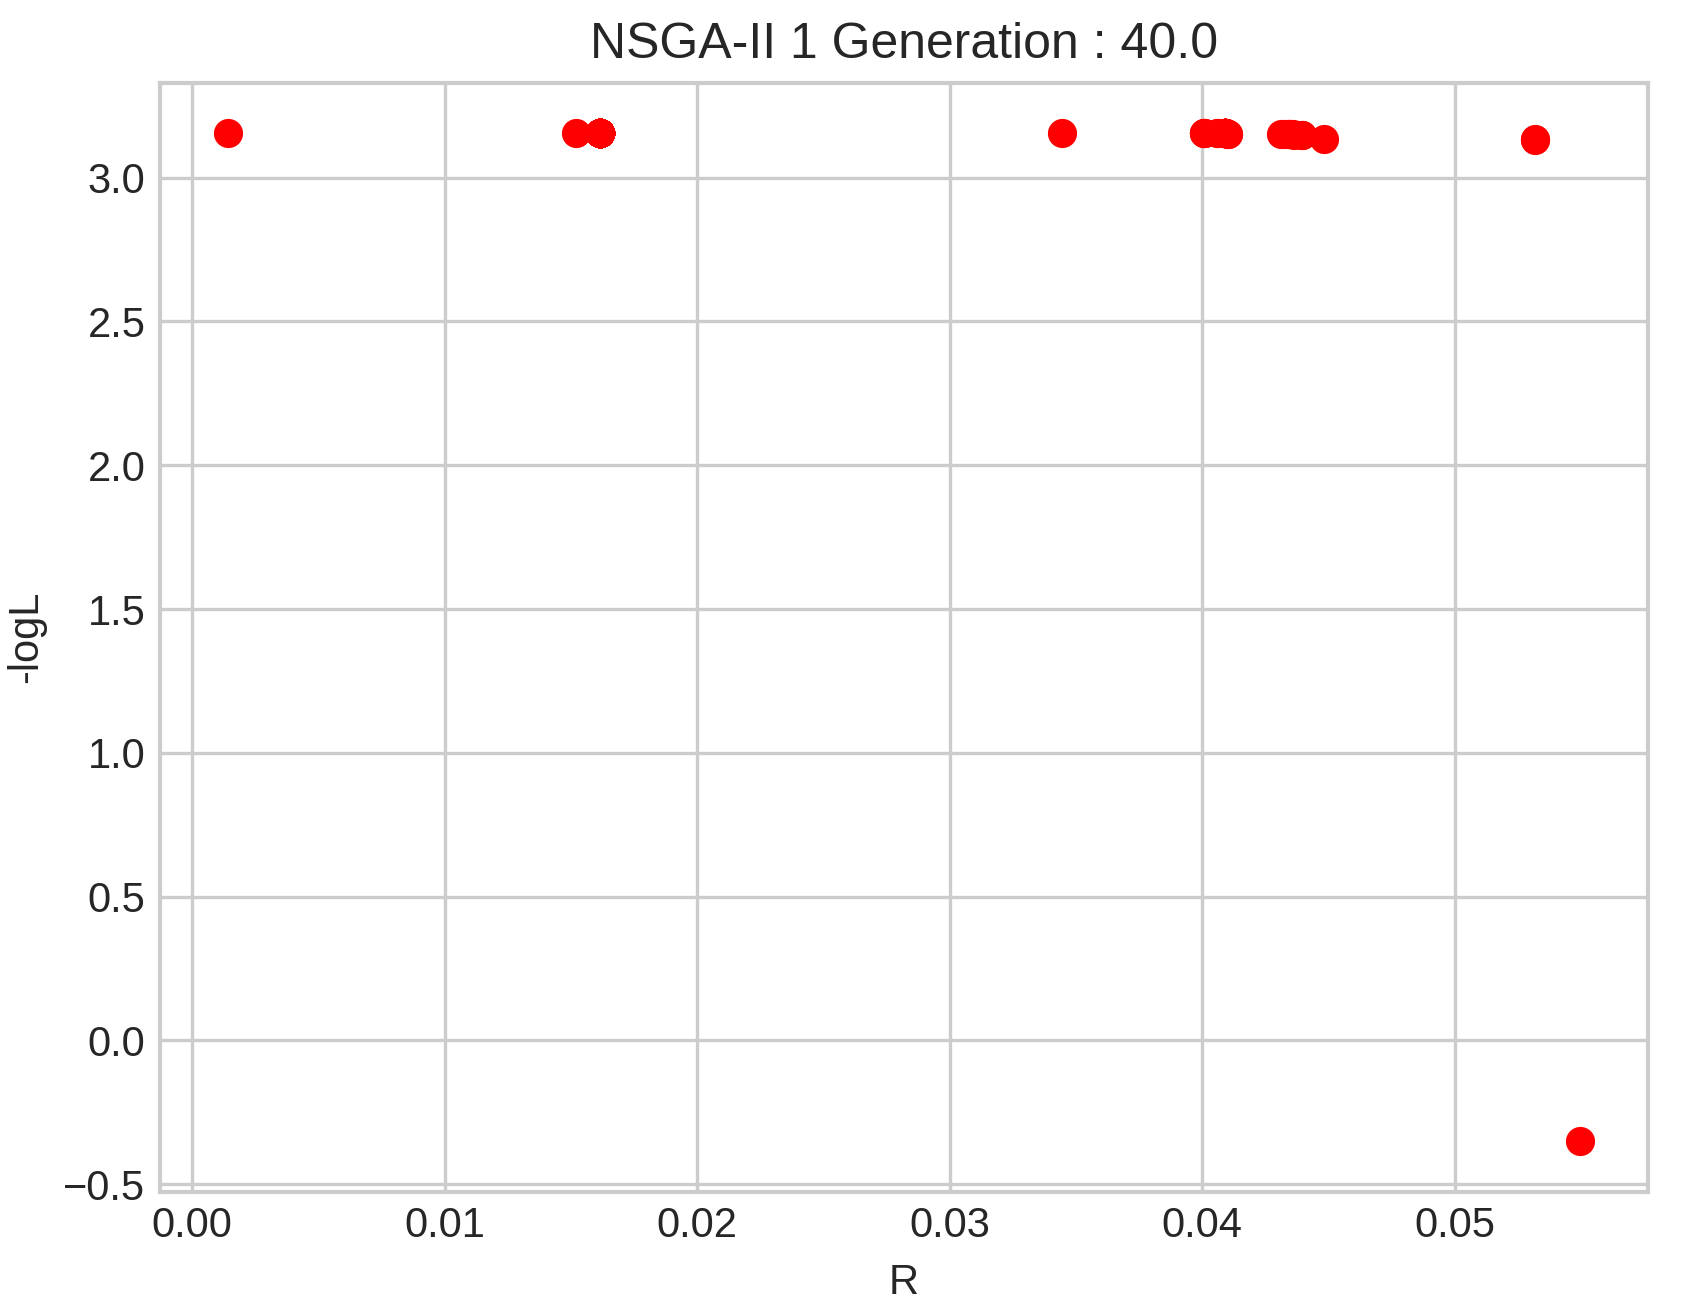
\includegraphics[width=\textwidth]{images/1-NSGA-II 1 Generation _ 40.0-R - logL-point.png}
  \end{figure}
  \end{minipage}
  \caption{Solutions scatter plot of NSGA-II Type 1 for generations 1,10,20,40}
  \label{fig:2x2group}
\end{figure}
\begin{figure}[H]
  \centering
  \begin{minipage}[b]{0.22\textwidth}
  \begin{figure}[H]
      \centering
      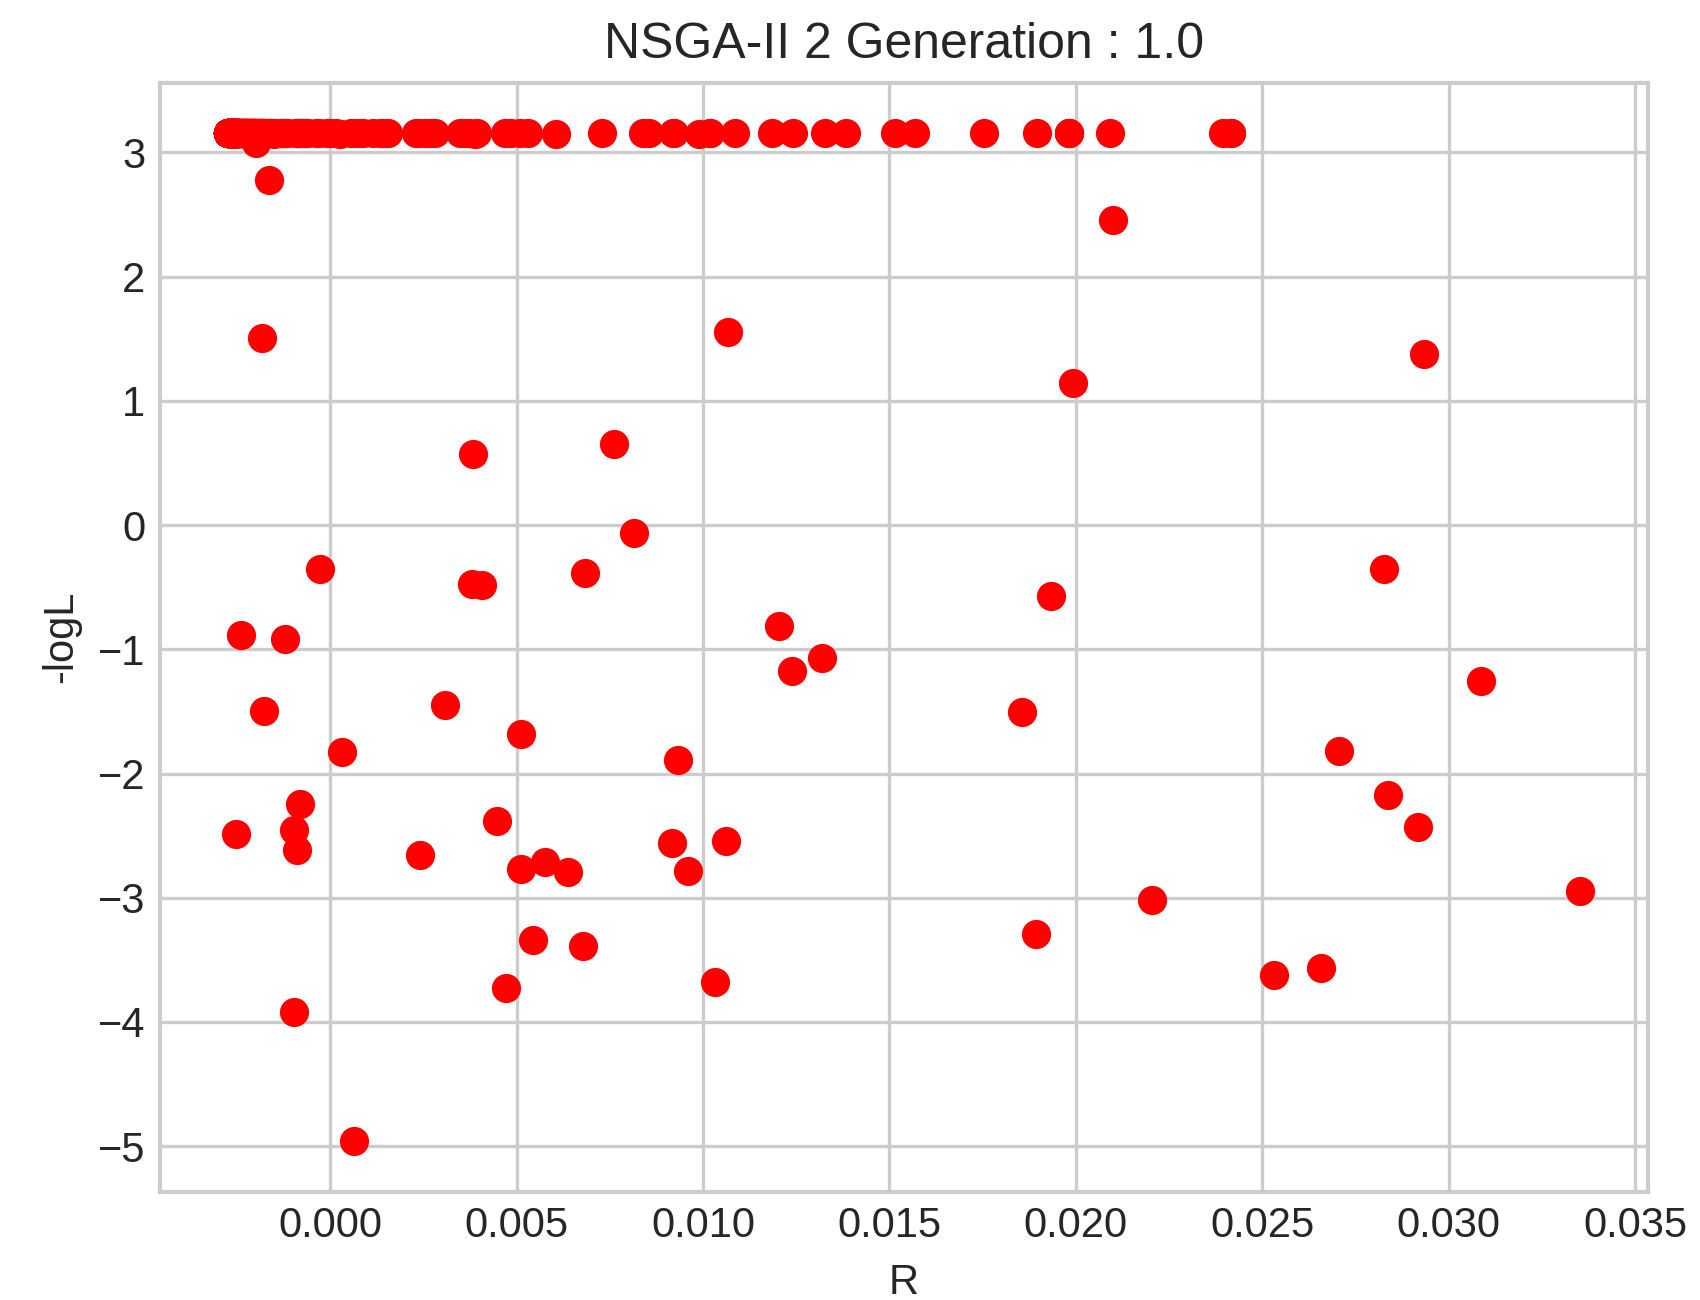
\includegraphics[width=\textwidth]{images/1-NSGA-II 2 Generation _ 1.0-R - logL-point.png}
  \end{figure}
  \end{minipage}
  \hspace{0.0cm}
  \begin{minipage}[b]{0.22\textwidth}
  \begin{figure}[H]
      \centering
      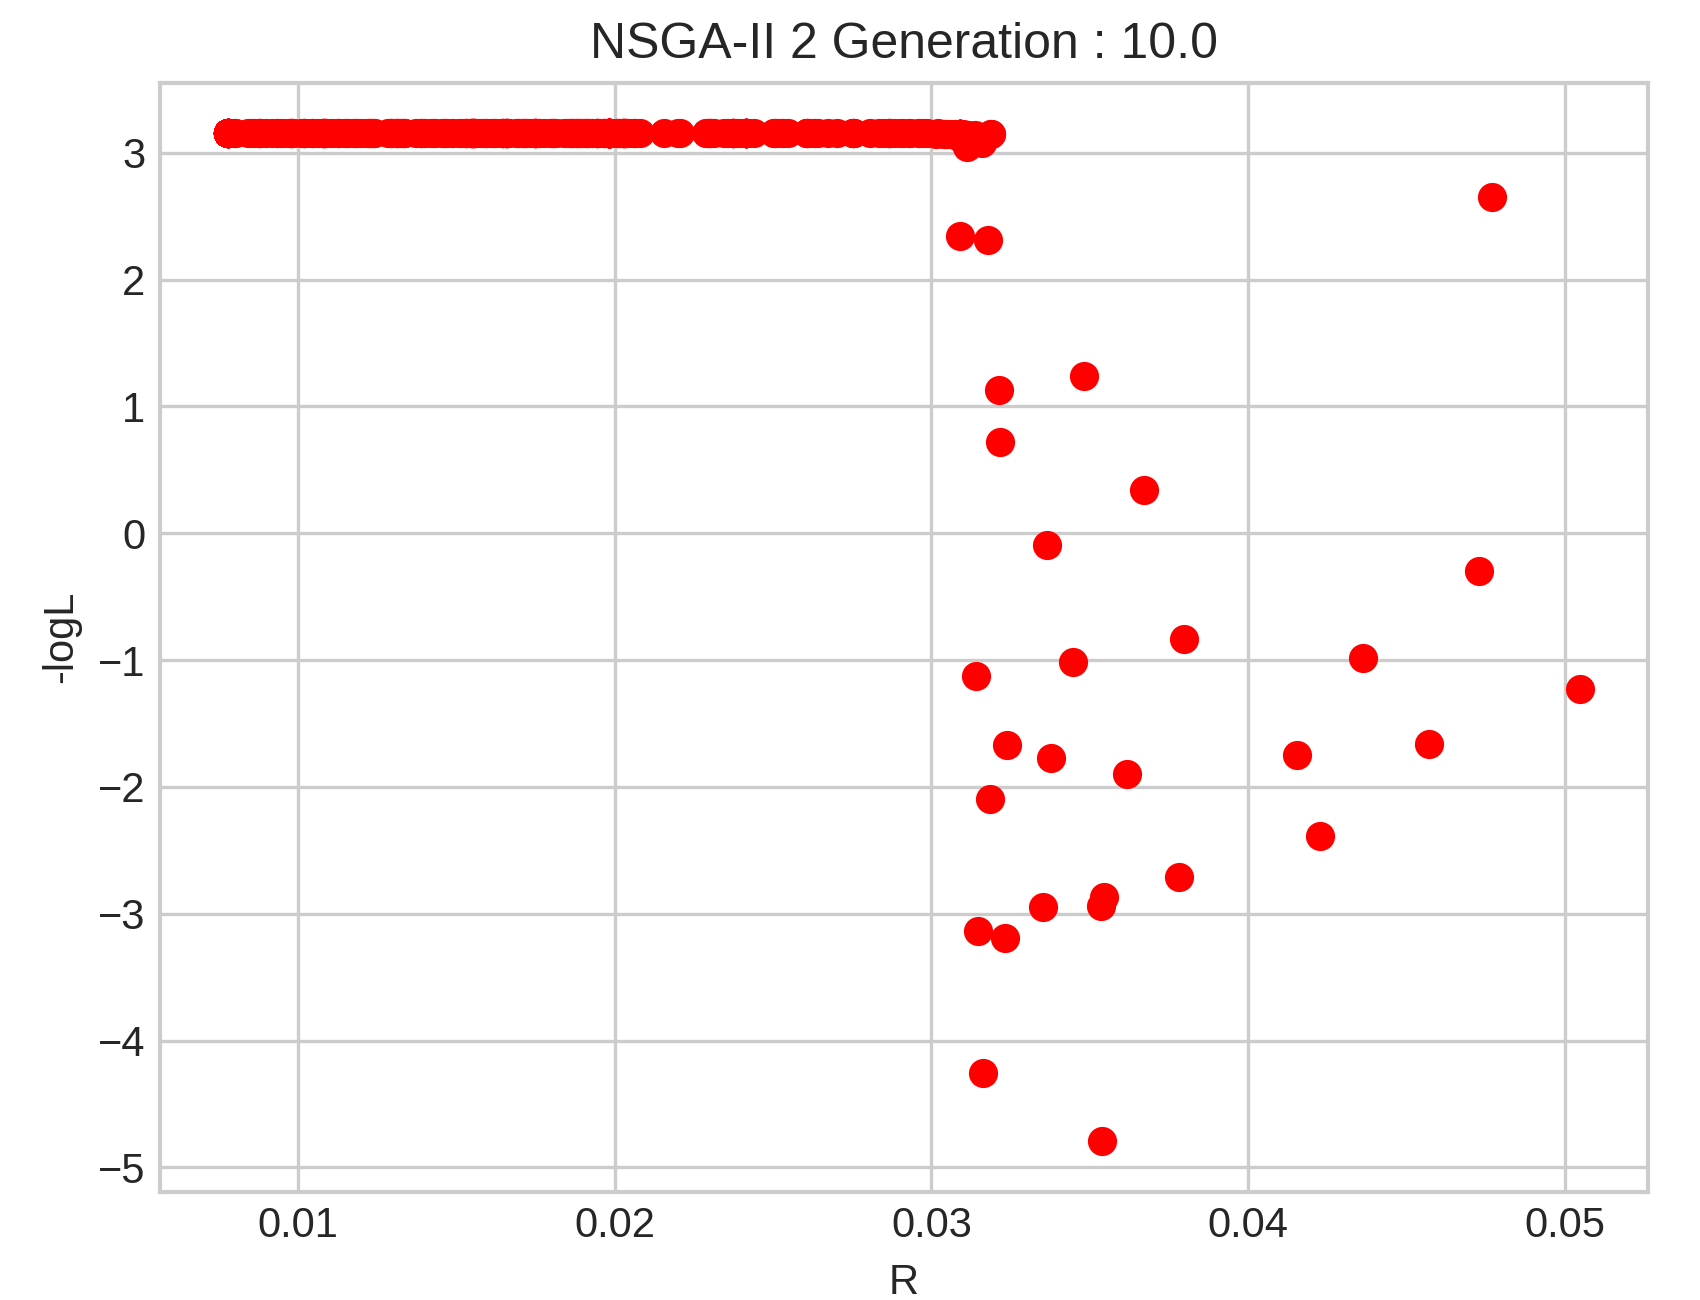
\includegraphics[width=\textwidth]{images/1-NSGA-II 2 Generation _ 10.0-R - logL-point.png}
  \end{figure}
  \end{minipage}
  \hspace{0.0cm}
  \begin{minipage}[b]{0.22\textwidth}
  \begin{figure}[H]
      \centering
      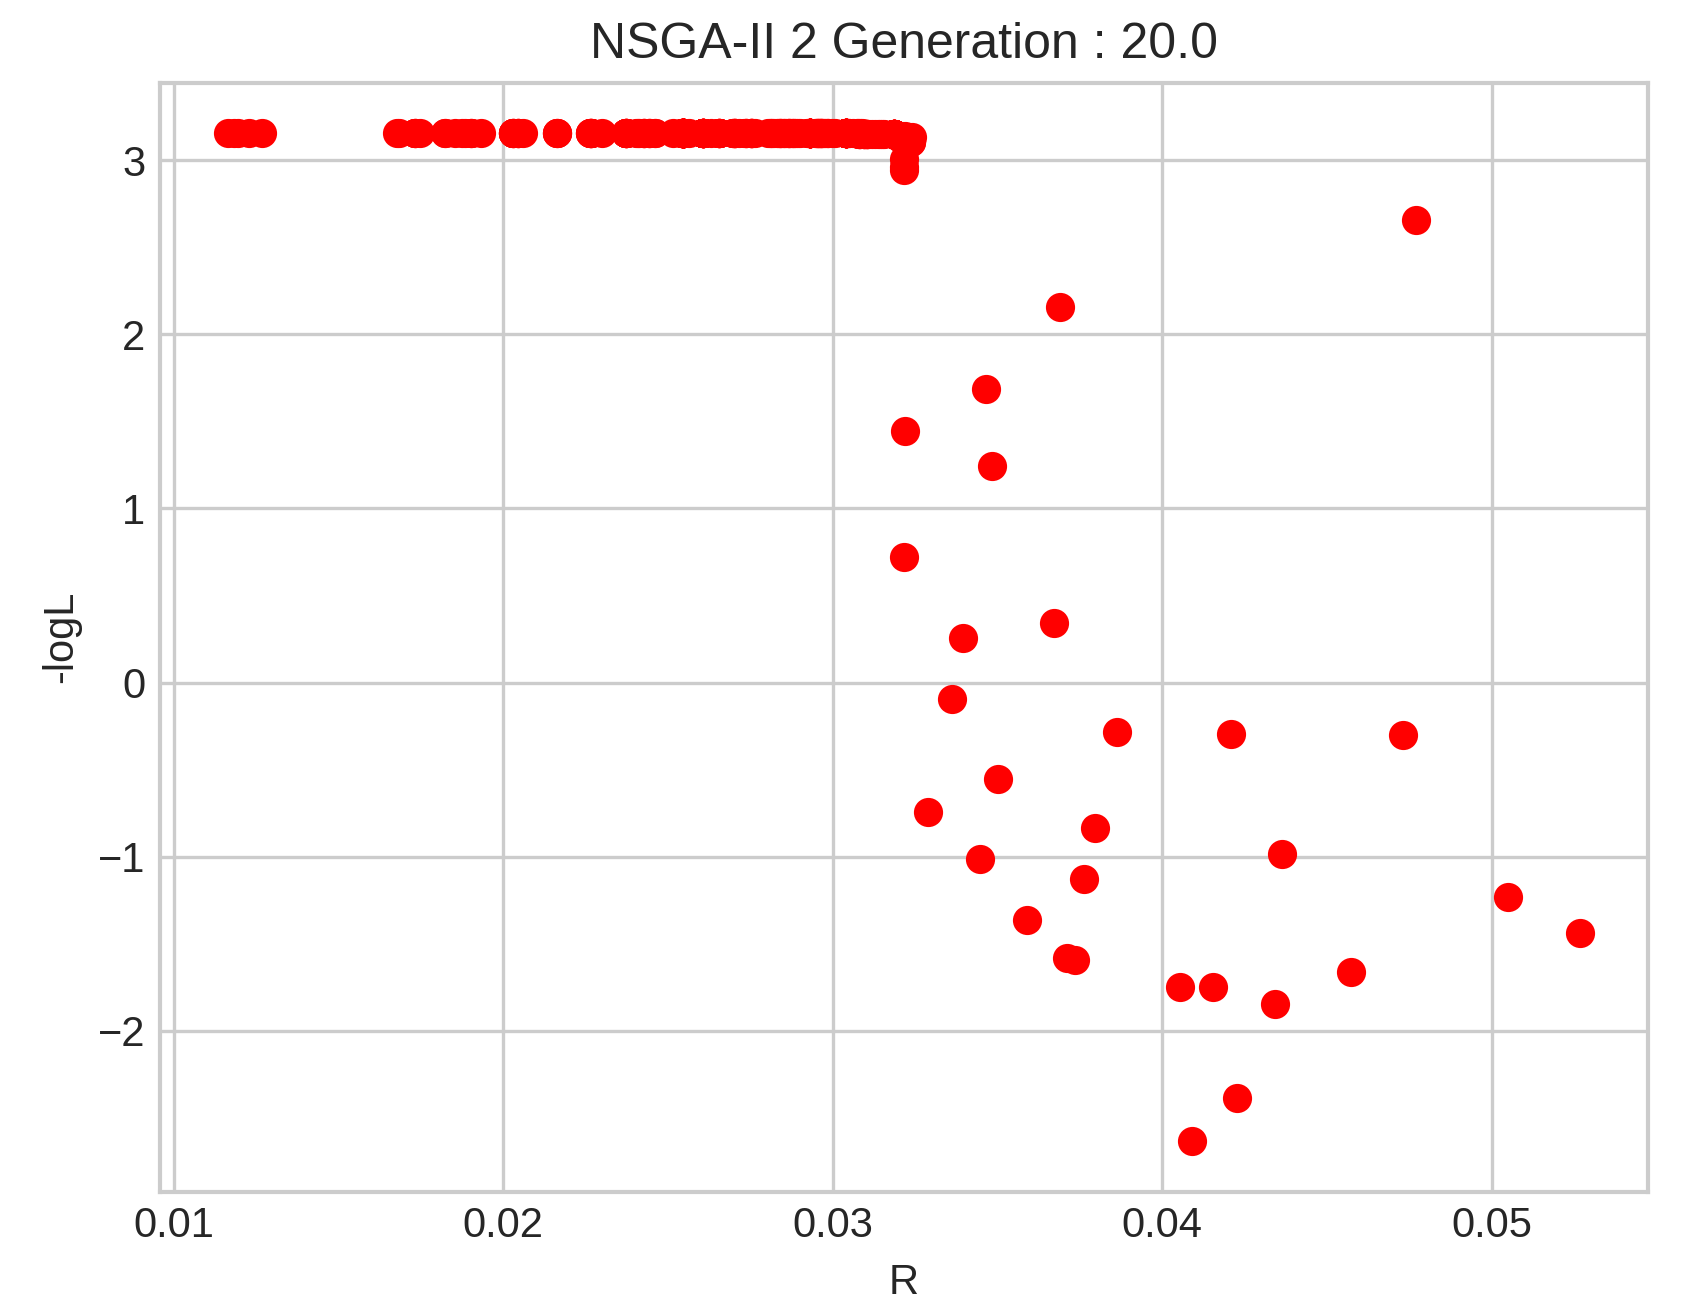
\includegraphics[width=\textwidth]{images/1-NSGA-II 2 Generation _ 20.0-R - logL-point.png}
  \end{figure}
  \end{minipage}
  \hspace{0.0cm}
  \begin{minipage}[b]{0.22\textwidth}
  \begin{figure}[H]
      \centering
      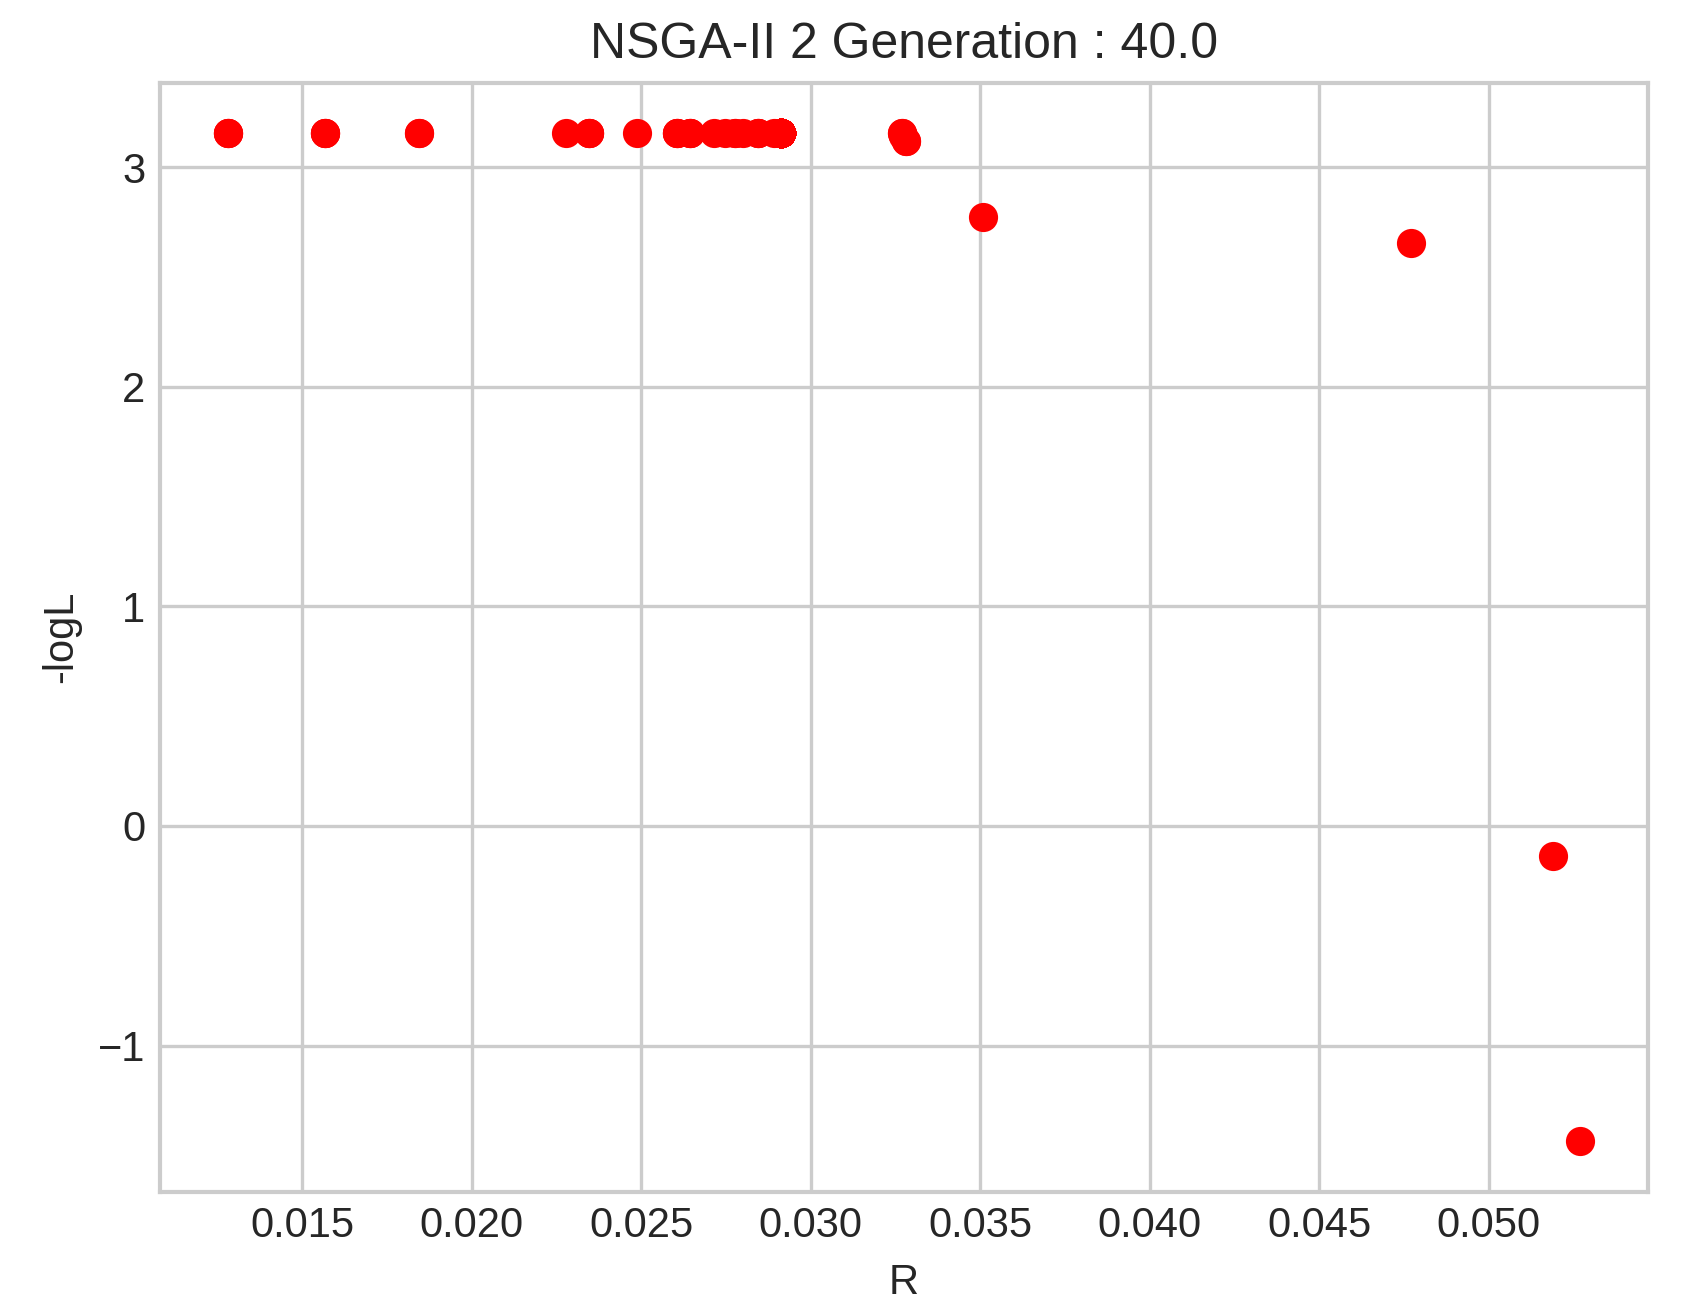
\includegraphics[width=\textwidth]{images/1-NSGA-II 2 Generation _ 40.0-R - logL-point.png}
  \end{figure}
  \end{minipage}
  \caption{Solutions scatter plot of NSGA-II Type 2 for generations 1,10,20,40}
  \label{fig:2x2group}
\end{figure}
\level{3}{MOPSO}
We executed MOPSO$(500,100,0.95,0.9,0.5,0.2,0.1,0.006)$, population size of 500 and 100 time iterations. We can observe that the solutions has swarm behavior, with a drift towards higher values of $R$, as a tradeoff, their $-log(L)$ value decreases.
\begin{figure}[H]
  \centering
  \begin{minipage}[b]{0.22\textwidth}
  \begin{figure}[H]
      \centering
      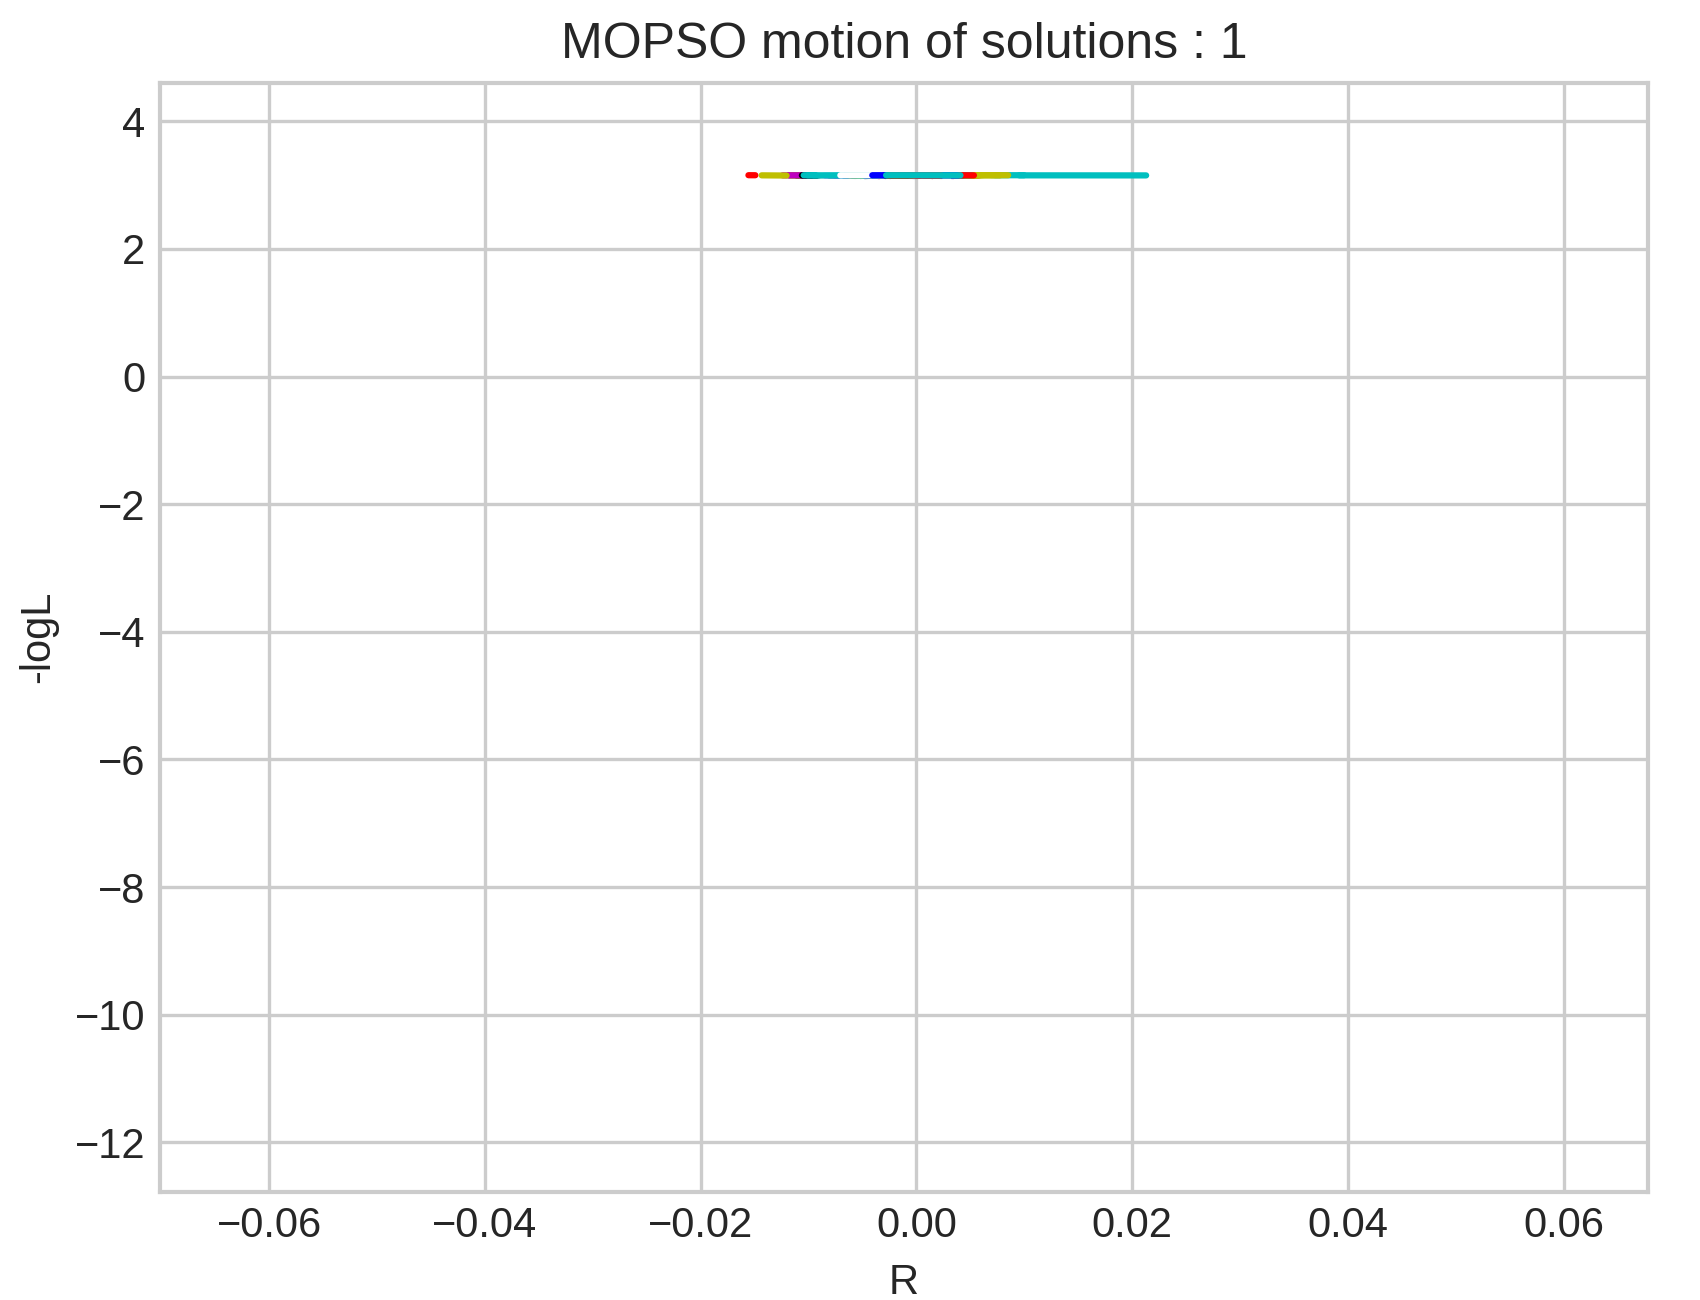
\includegraphics[width=\textwidth]{images/1-fix_axisMOPSO motion of solutions _ 1-R - logL-gard.png}
  \end{figure}
  \end{minipage}
  \hspace{0.0cm}
  \begin{minipage}[b]{0.22\textwidth}
  \begin{figure}[H]
      \centering
      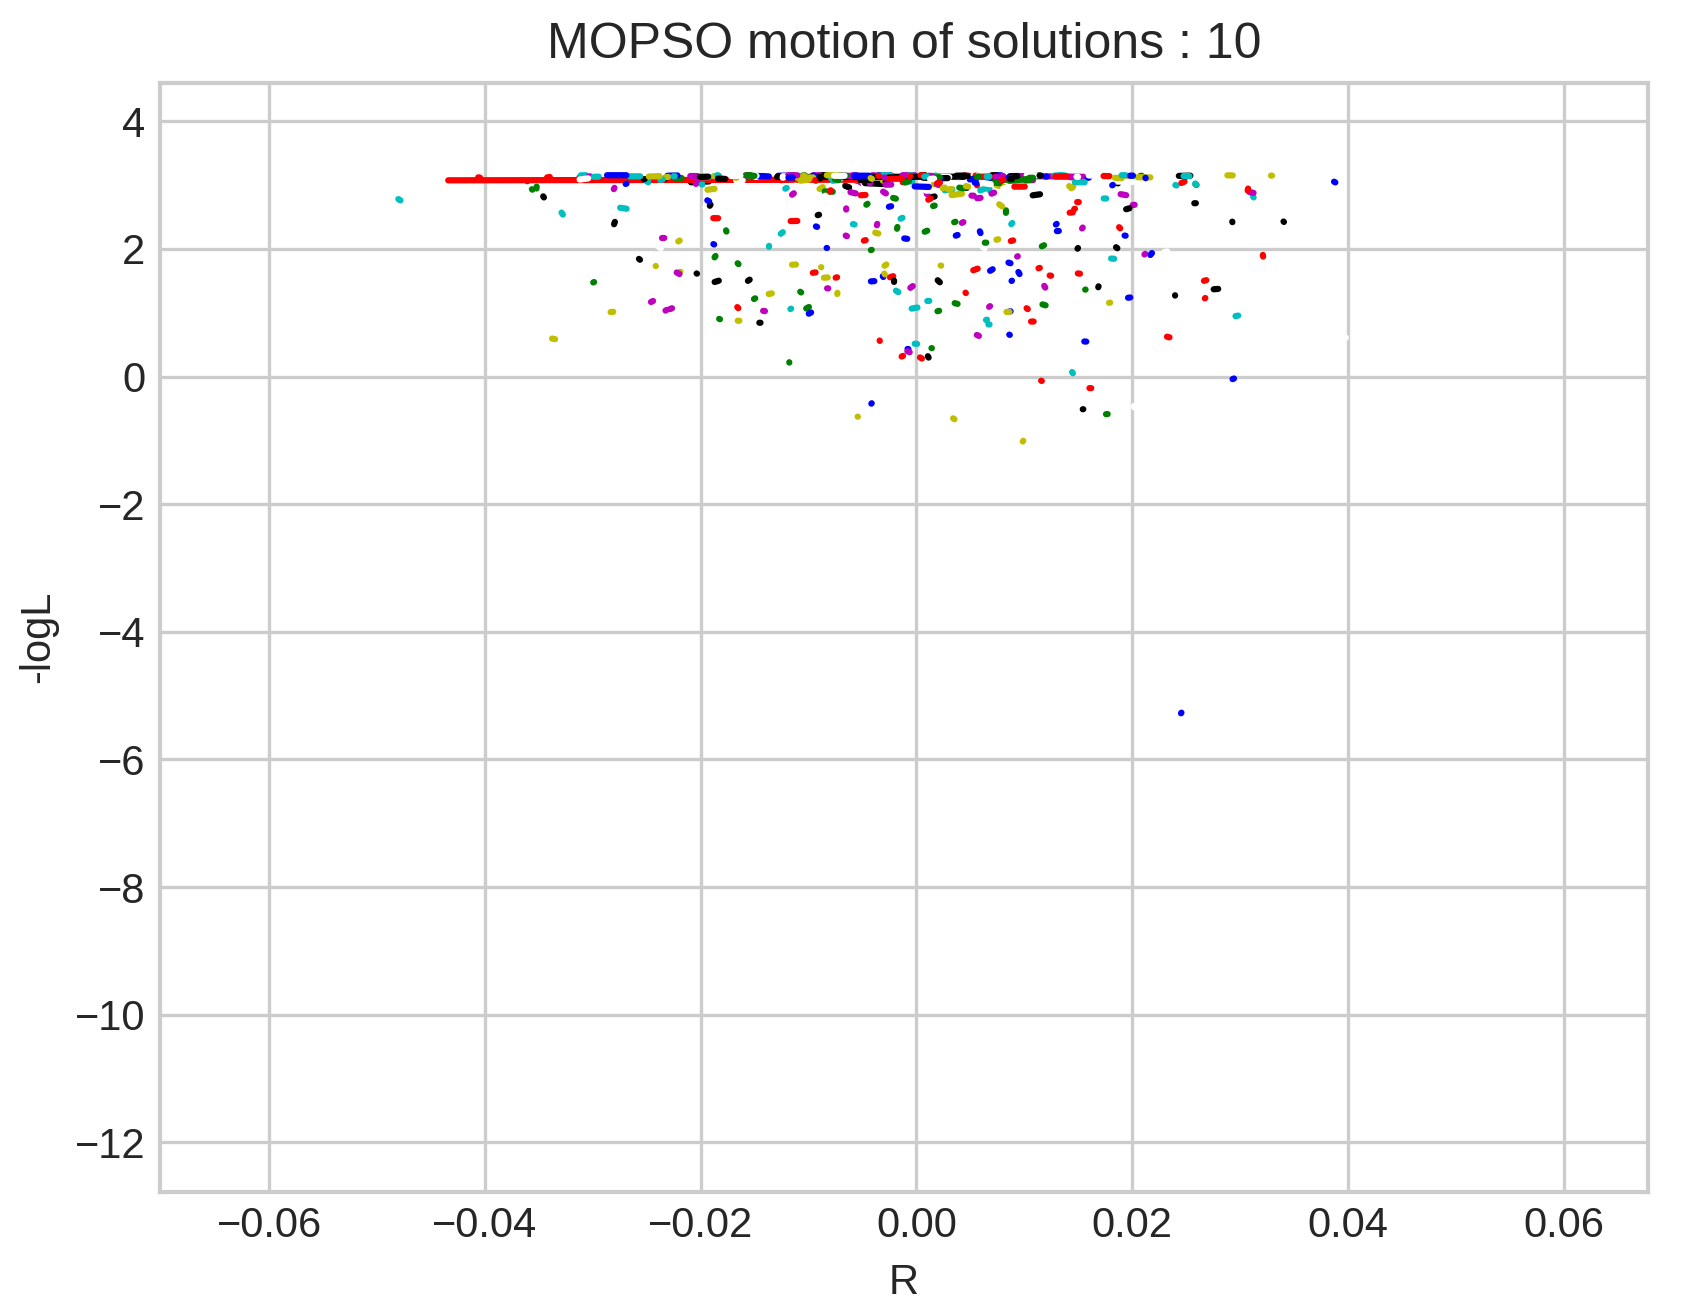
\includegraphics[width=\textwidth]{images/1-fix_axisMOPSO motion of solutions _ 10-R - logL-gard.png}
  \end{figure}
  \end{minipage}
  \hspace{0.0cm}
  \begin{minipage}[b]{0.22\textwidth}
  \begin{figure}[H]
      \centering
      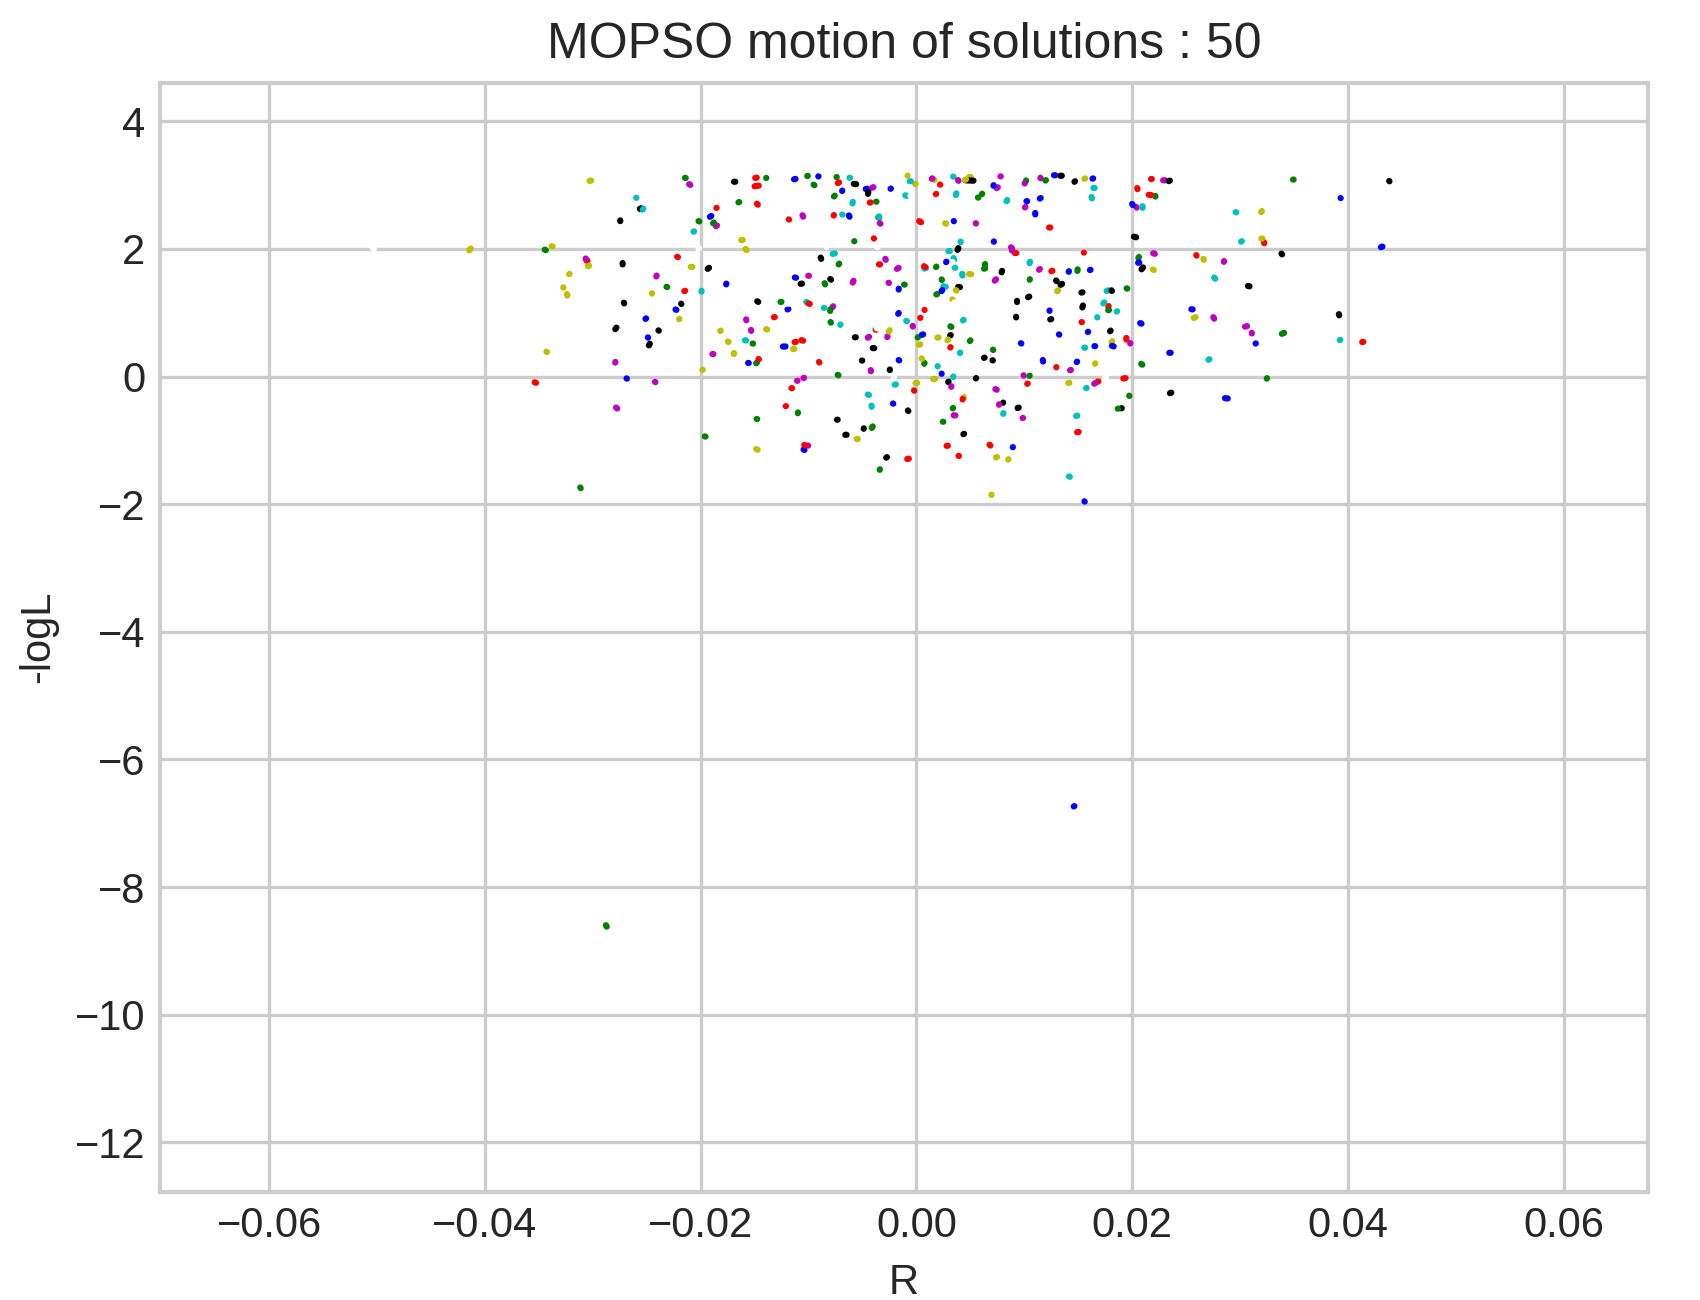
\includegraphics[width=\textwidth]{images/1-fix_axisMOPSO motion of solutions _ 50-R - logL-gard.png}
  \end{figure}
  \end{minipage}
  \hspace{0.0cm}
  \begin{minipage}[b]{0.22\textwidth}
  \begin{figure}[H]
      \centering
      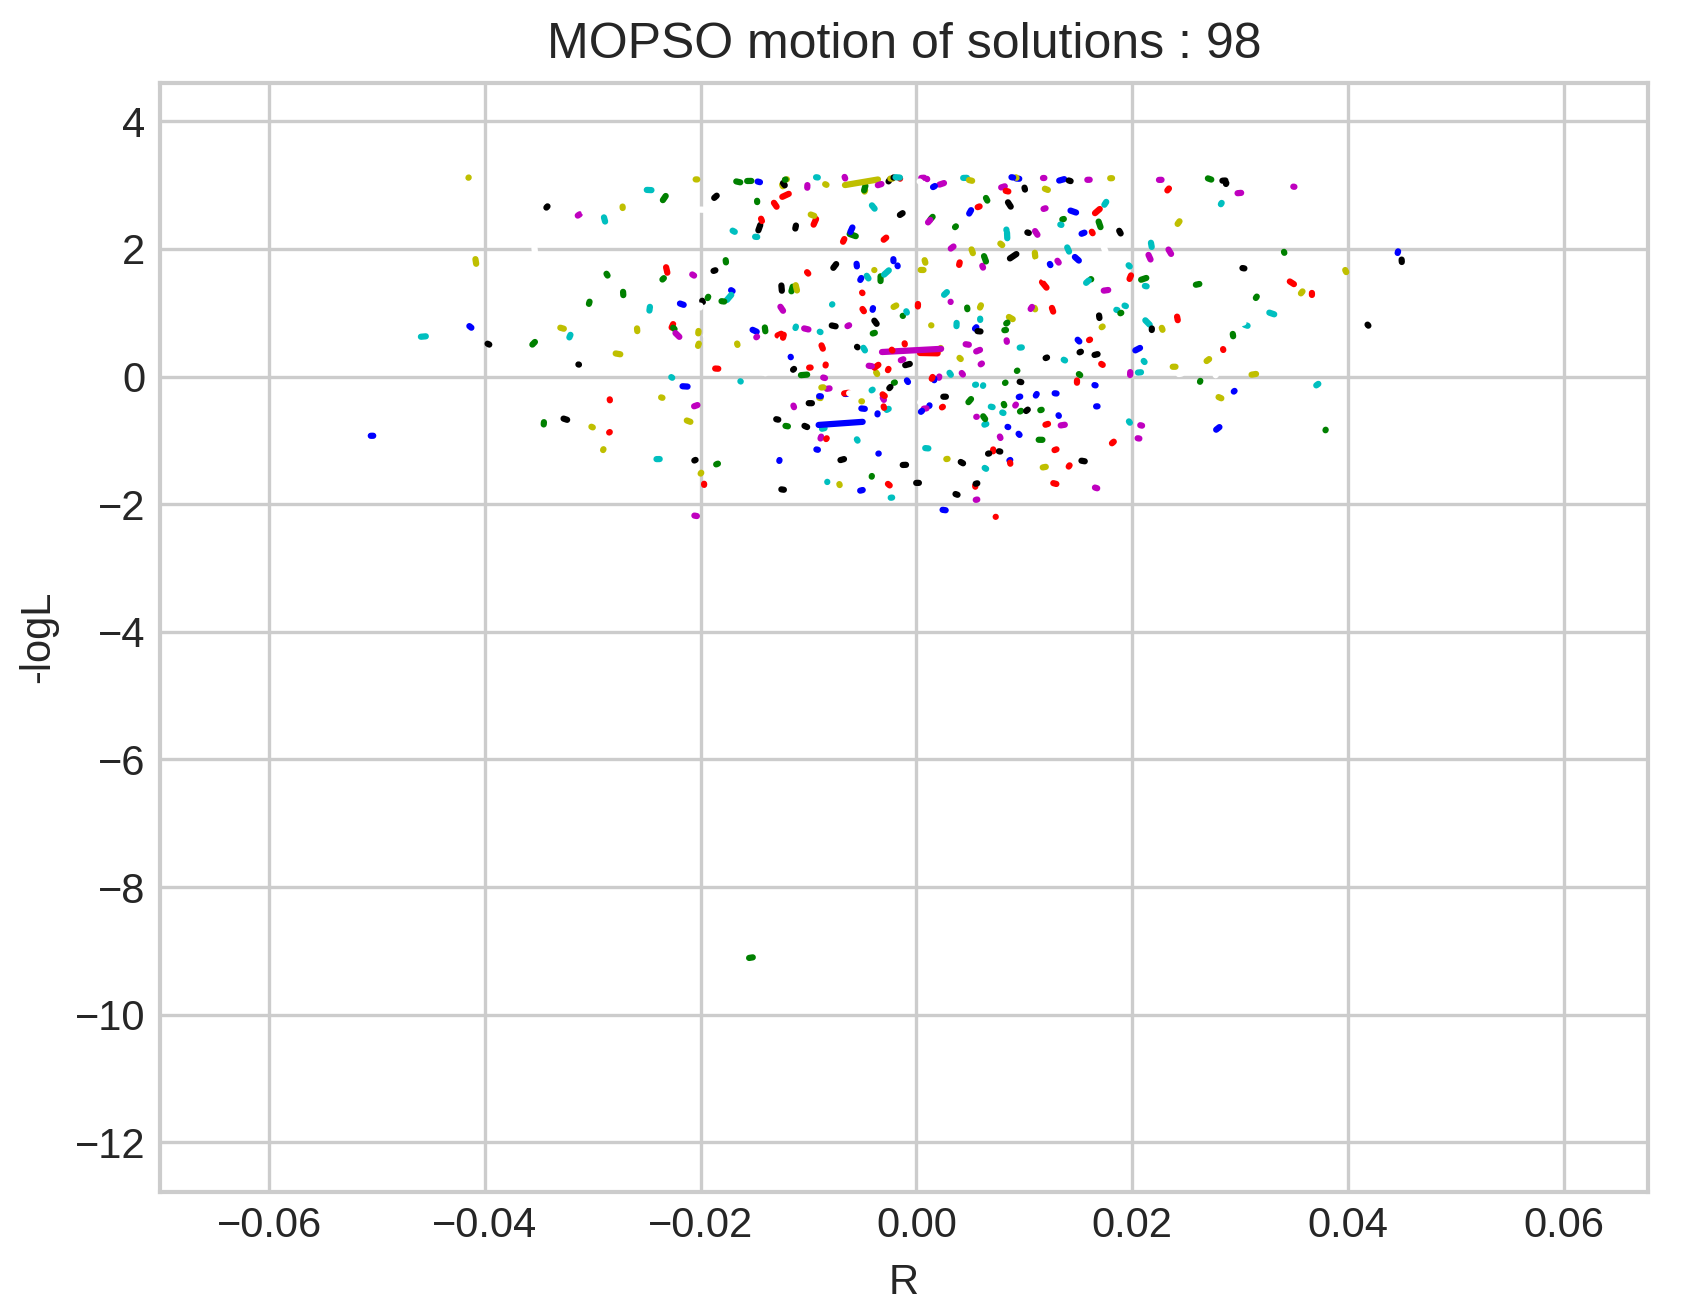
\includegraphics[width=\textwidth]{images/1-fix_axisMOPSO motion of solutions _ 98-R - logL-gard.png}
  \end{figure}
  \end{minipage}

  \caption{Solutions plot of MOPSO for time values of  1,10,50,98}
  \label{fig:2x2group}
\end{figure}

\level{3}{Comparison Table}

% \begin{sidewaystable}[htbp]
% \centering
% \begin{tabular}{|c|l|c|c|c|c|c|c|c|c|c|c|}
% \hline
% \multicolumn{1}{|c|}{Objective} & \multicolumn{1}{|c|}{Statistic} & \multicolumn{1}{|c|}{Baseline} & \multicolumn{2}{|c|}{OPI} & \multicolumn{2}{|c|}{DOI} & \multicolumn{2}{|c|}{NPM}& \multicolumn{2}{|c|}{NSGA-II} & \multicolumn{1}{|c|}{MOPSO} \\
%  & &  & Type 1 & Type 2 & Type 1 & Type 2 & Type 1 & Type 2 & Type 1 & Type 2 & \\
% \hline
%             & mean (1e-2)  & \textcolor{red}{-0.272} &  7.53 &  7.43 & 7.53 &  7.43 & \textbf{7.55} & \textbf{7.55} &  1.90 &  2.63 &  0.00266 \\
%             & std (1e-3)   &  2.36 &  3.43 &  4.48 & 1.85 &  3.23 & 1.42 & \textcolor{red}{1.41} &  9.38 &  7.60 &  \textbf{16.2} \\
%       $R$   & min (1e-2)   & -3.74 & -0.31 & -2.22 & 3.11 & -0.40 & \textbf{3.73} & 3.55 & -2.35 & -1.55 & \textcolor{red}{-5.86} \\
%             & 50\% (1e-2)  & -0.275 &  \textbf{7.56} &  7.47 & \textbf{7.56} &  7.47 & \textbf{7.56} & \textbf{7.56} &  1.62 &  2.91 & \textcolor{red}{-8.96} \\
%             & max (1e-2)   &  \textcolor{red}{4.00} &  \textbf{7.56} & \textbf{ 7.56} & \textbf{7.56} &  \textbf{7.56} & \textbf{7.56} & \textbf{7.56} &  5.51 &  5.93 &  5.63 \\
% \hline
%             & mean         & \textbf{3.15} & \textbf{3.15} & 3.14 & \textbf{3.15} &  \textbf{3.15} & \textbf{3.15} & \textbf{3.15} &  3.12 &  3.03 &  \textcolor{red}{1.42} \\
%             & std (1e-2)   & 2.51 & \textcolor{red}{0.00147} & 27.6 & 9.56 &  19 & 0.00155 & 0.00216 &  35.9 &  74.6 &  \textbf{146} \\
% $-log(L)$   & min          & 1.70 & \textbf{3.15} & -6.45 & 2.60 & -6.37 & \textbf{3.15} & \textbf{3.15} & -4.66 & -4.96 & \textcolor{red}{-11.3} \\
%             & 50\%         & \textbf{3.15} & \textbf{3.15} & \textbf{3.15} & \textbf{3.15} &  \textbf{3.15} & 3.1 & \textbf{3.15} &  \textbf{3.15} &  \textbf{3.15} &  \textcolor{red}{1.55} \\
%             & max          & \textbf{3.15} & \textbf{3.15} & \textbf{3.15} & \textbf{3.15} &  \textbf{3.15} & \textbf{3.15} & \textbf{3.15} &  \textbf{3.15} &  \textbf{3.15} &  \textbf{3.15} \\
% \hline
%             & mean   & \textbf{64.46} & 58.34 & 61.80 & 13.82 &  \textcolor{red}{10.06} & 61.58 & 27.22 & 63.60 & 64.15 & 63.38 \\
%             &  std   &  1.36 &  2.51 &  0.829 &  \textbf{9.54} &  5.98 &  0.75 &  4.19 &  0.52 &  \textcolor{red}{0.37} &  0.95 \\
% $-log(O)$   & min    & 56.41 & 54.09 & 60.5 & -6.56 & \textcolor{red}{-6.65} & \textbf{60.06} & 12.43 & 56.32 & 58.47 & 59.65 \\
%             & 50\% & \textbf{64.68} & 57.84 & 61.6 & 16.21 &  \textcolor{red}{14.4} & 61.46 & 29.01 & 63.54 & 64.09 & 63.42 \\
%             & max    & \textbf{67.50} & 66.32 & 66.61 & 24.46 &  \textcolor{red}{14.96} & 66.42 & 29.74 & 66.98 & 66.88 & 67.29 \\
% \hline
% \end{tabular}
% \caption{Statistics on solutions generated by various method}
% \label{tab:stat_table}
% \end{sidewaystable}

\begin{figure}[H] \label{fig:results-table}
\centering
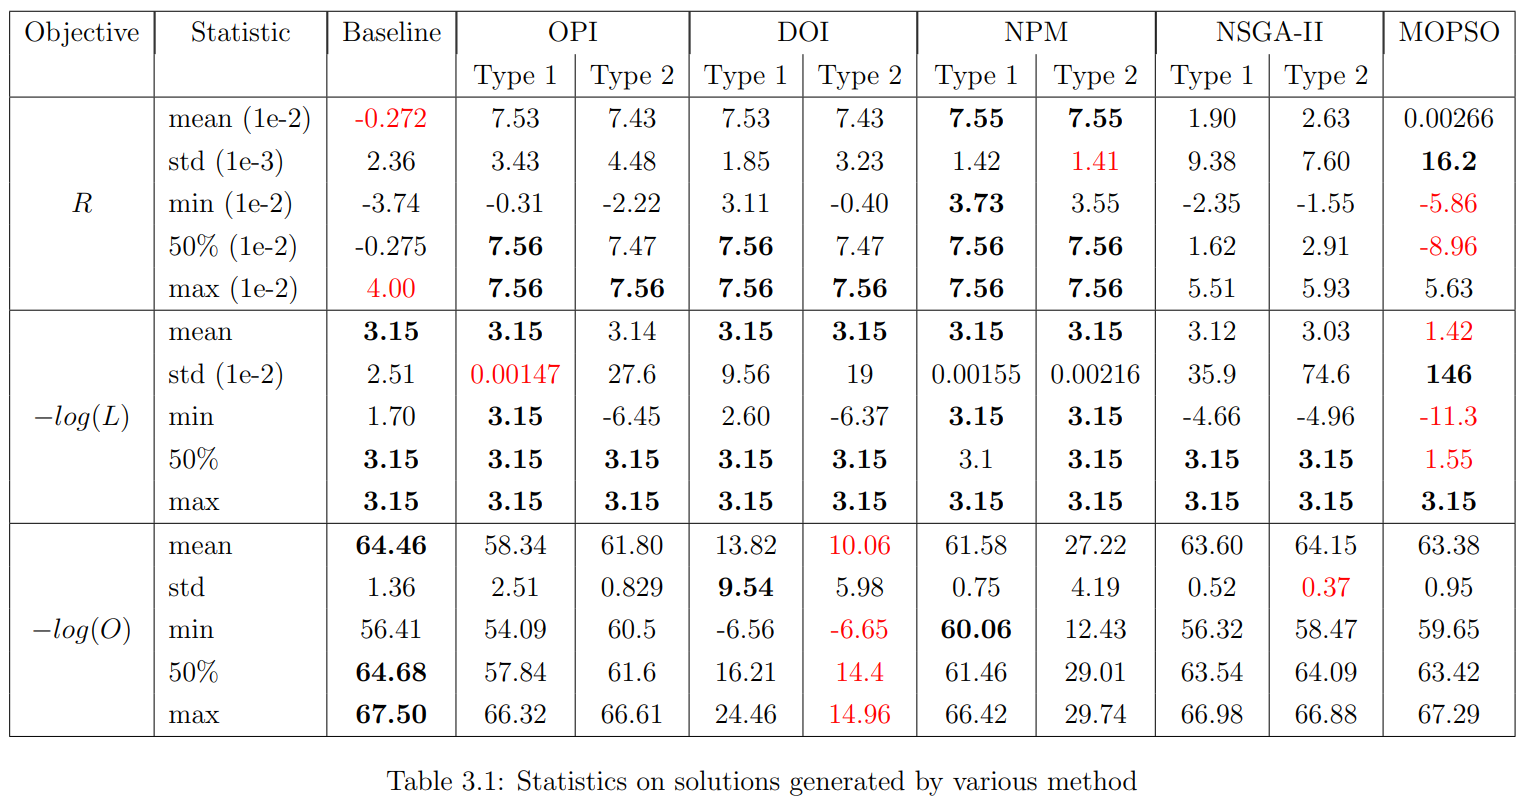
\includegraphics[width=1.0\textwidth]{images/results-table.png}
\end{figure}

\level{3}{Discussion}

We note that the baseline method provides a basis for comparison with other methods. Methods that have high mean values and low variance values are considered good, as they converge more quickly towards the optimum. When considering the distribution of $-log(L)$, we observe that all methods, except for MOPSO, have a distribution that is very close to optimal. Additionally, we note that most of the standard deviation in the values of $-log(L)$ is found in the latter decimals of the values. As a result, there is no significant difference in the first two digits after the decimal point. However, we do observe that MOPSO performs particularly poorly, with a high standard deviation. Additionally, we note that both DOI types, OPI type 2, and both NSGA-II types have slightly higher standard deviations. Regarding $R$, we note that all methods except NSGA-II and MOPSO achieve the maximum value. However, among the methods that achieve the maximum value, OPI type 1, DOI type 1, and both NPM types achieve it more efficiently, as their 50\% value is the same. Moreover, the NPM methods have the lowest variation among them. Regarding $-log(O)$, we observe that the baseline method has the highest values. We also note that the methods that perform well with higher $R$ generally have lower values of $-log(O)$.




















% \newpage
% %%% ADVERSARIAL NETWORK
% \level{2}{Problem: Defense Against Adversarial Attack} \label{results_problem_2} 
% \hspace{6mm} A dataset of $n$ images ${(X_1, y_1), (X_2, y_2), ..., (X_n, y_n)}$, where $X_i$ represents an image and $y_i$ represents its corresponding label, the task is to develop a function $N(X_i; \theta)$ that takes an image $X_i$ as input and predicts its label $y_i$ using a set of model parameters $\theta$.
% \newline Formally, the task is to find the optimal set of parameters $\theta^*$ that minimizes the following loss function:
% \begin{equation} \label{problem_daaamd_opt_thita_expression}
%     \theta^* = \arg\min_\theta \frac{1}{n}\sum_{i=1}^n L(N(X_i; \theta), y_i)
% \end{equation}
% \newline where $L$ is a loss function that measures the difference between the predicted label and the true label.

% An adversarial attack is a perturbation $\delta$ added to the original input image $X_i$ to produce a new image $X_i' = X_i + \delta$ that is designed to cause misclassification of the model. The goal of the attacker is to find the perturbation $\delta$ that maximizes the difference between the predicted label and the true label.
% \newline Formally, the task is to find the optimal perturbation $\delta^*$ that maximizes the following objective function:
% \begin{equation} \label{problem_daaamd_adv_delta_expression}
%     \delta^* = \arg\max_\delta L(N(X_i + \delta; \theta), y_i)
% \end{equation}
% \newline where $L$ is a loss function that measures the difference between the predicted label and the true label.

% \level{3}{Data}
% The MNIST dataset consists of 60,000 grayscale images of handwritten digits (0-9) with a resolution of 28x28 pixels. There is an additional test set of 10,000 images. Each image is labeled with its corresponding digit. The pixel intensity values of the images in the MNIST dataset range over integer values from 0 to 255. 
% \newline 
% The MNIST dataset is a widely used benchmark dataset in the field of machine learning, and many different models have been developed to classify the digits in this dataset. However, it has been shown that these models are vulnerable to adversarial attacks, which can cause them to misclassify images with high confidence.

% \begin{figure}[H]
%   \centering
%   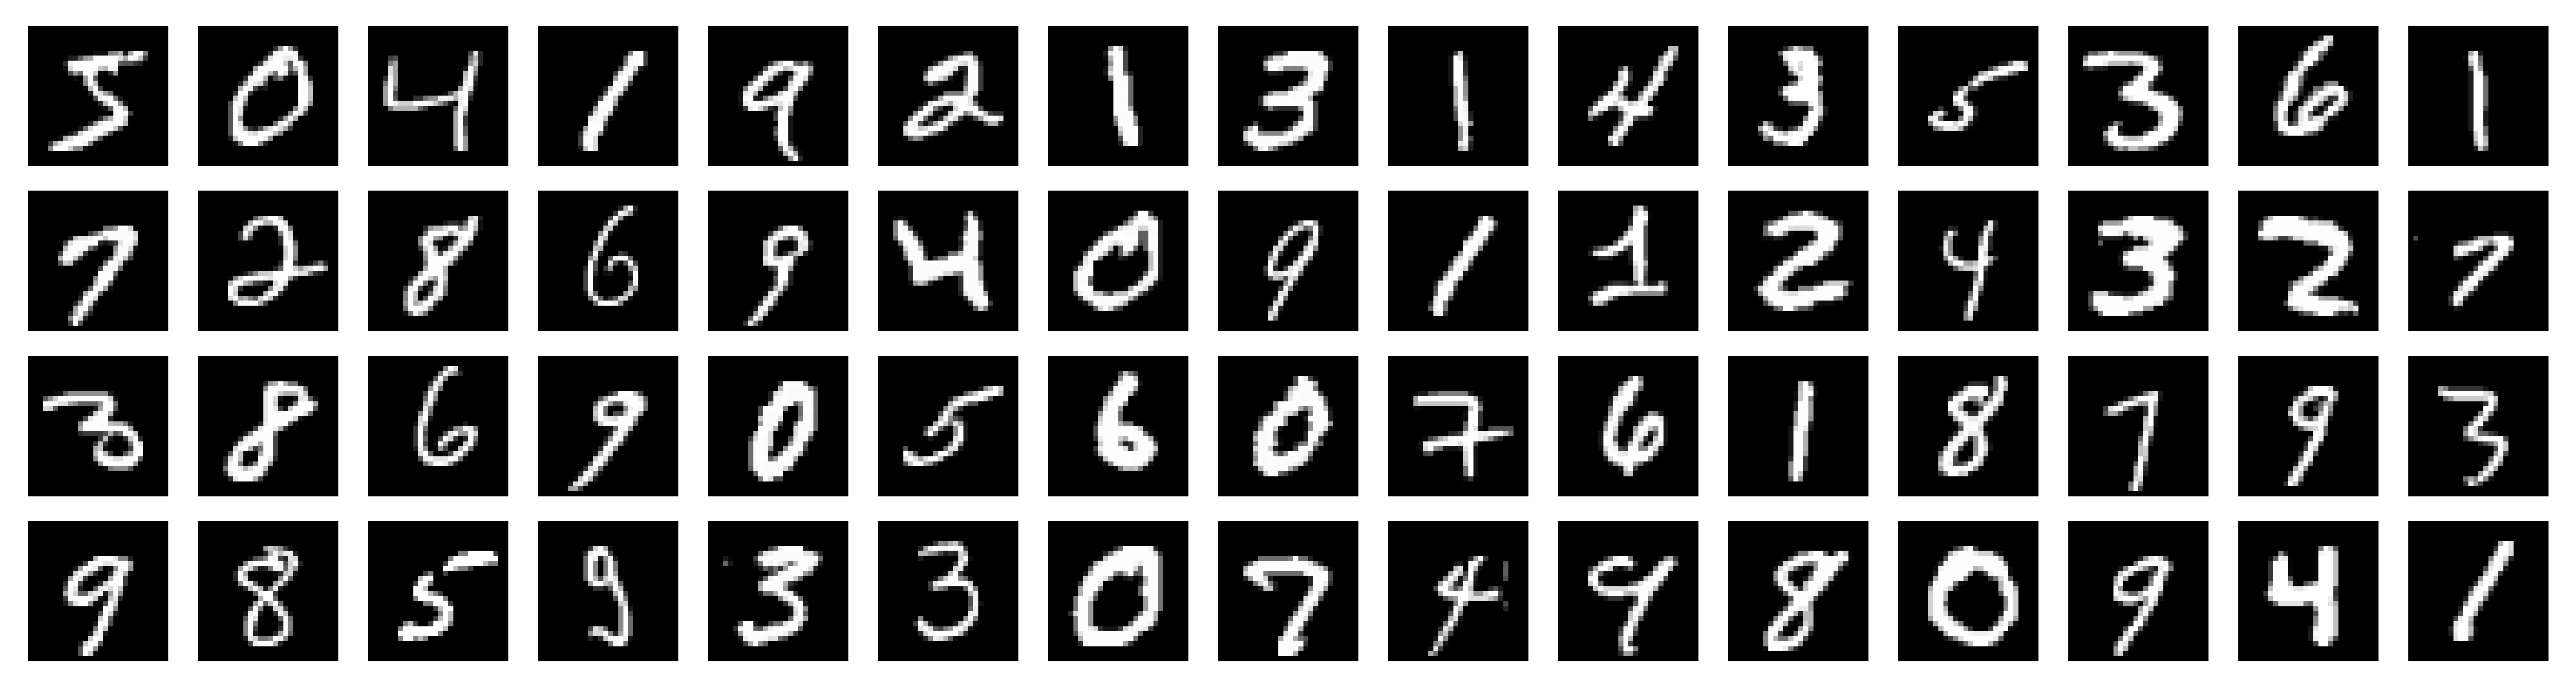
\includegraphics[width=0.9\textwidth]{images/mnist_60_images_4x15_grid.png}
%   \caption{Images from the MNIST training set.}
%   \label{fig:mnist_images}
% \end{figure}

% \level{4}{Preprocessing }

% \level{3}{Approaches}
% \level{4}{Linear Classifier}
% \level{4}{Linear Classifier with $L_2$ Norm}
% \level{4}{Linear Classifier with $\kappa_2$ Minimization}



% \chapter{Experiments and Results}
Here write about the work that you have done. The title of this chapter/section may vary depending on the
problem of your project. You may add some subsection like methods and data set etc. as follows.
The experiments were conducted using Pytorch
\textbf{\cite{paszke2019pytorch}} and Hugging Face’s transformers \textbf{\cite{wolf2020huggingfaces}}. For all the experiments in this paper, we used 48-core Xeon processor Linux based system with 126 GB RAM. For training  the  neural networks  we  used 2 NVIDIA P100 GPUs having 16 GB each with CUDA version 10.1. We primarily based our system on Python libraries. Among the neural networks we used Huggingface's transformers library\footnote{https://huggingface.co/} for GPT-2 based models with PyTorch as backend in general. All the libraries used in this research are pip installable. Further we also resort to the code which controls the generation using \textsc{GeDi} models and the code which trains the \textsc{GeDi} models from the authors' git repository\footnote{https://github.com/salesforce/GeDi}.

\section{Evaluation Metrics}

We consider several metrics to evaluate our whole pipeline of controlled counterspeech generation. The \textit{generation metrics} measure the generation capability of the DialoGPTm and \textsc{GeDi} models. The \textit{classification metrics} are mainly to evaluate the \textsc{GeDi} model on the attribute datasets. Finally, we measure the amount of control in the generated counterspeech using external classifiers which we refer to as \textit{controller metrics}. We generate 5 samples for every hate speech instance with DialoGPTm. The GPS framework automatically selects the best response based on the heuristic, hence we keep one sample for every hate speech instance.

\newpage

\noindent\textbf{Generation metrics}: To measure the generation quality, we use different standard metrics. We use \textit{BLEU}, \textit{BLEU-4}~\cite{papineni2002bleu} and \textit{METEOR}~\cite{banerjee2005meteor} to measure how similar the generated counterspeech are to the ground truth counterspeech. While BLEU measures precision based on 1 to n-grams, METEOR measures the harmonic mean of unigram precision and recall. We also measure if the generation model generates a diverse and novel counterspeech. For this purpose, we use the diversity and novelty metrics from previous research~\cite{wang2018sentigan}.\newline


\noindent\textbf{\textsc{GeDi} metrics}: For classification, we report \textit{accuracy}, \textit{macro F1-score}, and \textit{AUROC} score for each \textsc{GeDi} model's performance on a test dataset of a particular attribute. We also report the generation performance using the perplexity~\cite{zhang2020dialogpt}.\newline


\noindent\textbf{Controller metrics}: In order to evaluate the ability of the \textsc{GeDi} controller to control the attribute, we used third-party classifiers for each attribute. For politeness, we trained a bert-base-uncased model for politeness level detection on a scale of 0 to 7\footnote{\footnotesize https://github.com/AlafateABULIMITI/politeness-detection}. For measuring emotion in the generated text, we used the Ekman version of the GoEmotions models\footnote{\footnotesize https://huggingface.co/monologg/bert-base-cased-goemotions-ekman}. For each post, it returns a confidence score between 0-1 for anger, disgust, fear, joy, sadness, surprise + neutral.  We report the confidence score for a particular emotion as a measure of that emotion in a given post. Finally, to measure toxicity we used the HateXplain model~\cite{mathew2020hatexplain} trained on two classes -- toxic and non-toxic\footnote{\footnotesize https://huggingface.co/Hate-speech-CNERG/bert-base-uncased-hatexplain-rationale-two}. We report the confidence between 0-1 for the non-toxic class.



\section{Generation results} 
We compare DialoGPTm model with the generate, prune and select pipeline (GPS) in Table \ref{tab:results-accurate}. We find \textbf{BLEU} and ~\textbf{BLEU4} for the GPS model is better than the DialoGPTm model for two out of three datasets. This might be due to the response selection part which focuses on selecting the semantically similar counterspeech to hate speech. On the other hand, all other scores are higher for the DialoGPTm for all the three datasets. DialoGPTm presents a competitive performance compared to the state-of-the-art model. For the rest of the experiments, we therefore use DialoGPTm. 
% \bm{I can understand why the results are like what they are, but does it make sense? The ground truth was generated based on guidelines which had nothing to do with attributes. For DialogGPTm this is basically an uphill battle. It's almost sure to lose and it has to generate a sentence closer to the ground truth while trying to maintain the attribute properly. This additional constrain is not present in the ground truth so GPS is bound to perform better. That would also explain the other 3 metrices result.}

% \bm{If we are going to report this, we should atleast justify why our model underperforms.}
\newpage
\begin{table}[!htpb]
\centering
\scriptsize
\begin{tabular}{|c|c|c|c|c|c|}
\hline
Model & B ($\uparrow$) & B4 ($\uparrow$) & M ($\uparrow$) & N ($\uparrow$) & D ($\uparrow$)\\
\hline
\multicolumn{6}{|c|}{\textbf{CONAN}}                                   \\ \hline

GPS & 0.46 & 0.46 & 0.14  & 0.18 & 0.60  \\
DialoGPTm & \textbf{0.50}& \textbf{0.50}& \textbf{0.18} &\textbf{ 0.84} & \textbf{0.80} \\\hline

\multicolumn{6}{|c|}{\textbf{Reddit}}                                   \\ \hline

 GPS & \textbf{0.36} & \textbf{0.36} & 0.11 & 0.30 & 0.47  \\
 DialoGPTm & 0.23 & 0.23 & \textbf{0.17} & \textbf{0.82} & \textbf{0.74} \\\hline

\multicolumn{6}{|c|}{\textbf{Gab}}                                   \\ \hline
           

GPS & \textbf{0.36 }& \textbf{0.36} & 0.12 & 0.15  & 0.41 \\
DialoGPTm & 0.26 & 0.26 & \textbf{0.17} & \textbf{0.80} & \textbf{0.72} \\
\hline
\end{tabular}
\caption{\scriptsize{Evaluation results for the three datasets. We report BLEU (B), BLEU4 (B4), METEOR (M), novelty (N) and diversity (D) to compare the two baselines: generate-prune-select (GPS) framework and DialoGPTm. For all metrics, higher is better.}}
\label{tab:results-accurate}
\end{table}

\noindent\textbf{\textsc{GeDi} metrics}: As reported in Table \ref{tab:attribute-performance}, we find that F1-score and AUCROC scores for politeness and all the four emotions are above 0.9 . This highlights that even with $0.2$ as the weight for the discriminator we are able to get good scores on classification. The perplexity scores for all the test datasets are also around $3.5$\footnote{For reference, perplexity for pretraining GPT-2 comes around 10 after 10K steps (https://tinyurl.com/3vwrvscd)}. \textsc{GeDi} model for toxicity has lower scores than the other attribute tasks. The F1-score for toxicity detection is $\sim0.6$ and AUCROC is $\sim 0.83$. The perplexity is also higher at around $4.5$ for the toxicity dataset. This highlights the difficulty of the task of detecting toxicity.
\begin{table}[h!]
\scriptsize
\centering
\begin{tabular}{cc|c|c|c|c}
\hline
\textbf{Dataset} & \textbf{Positive} & \textbf{F1} ($\uparrow$) & \textbf{Acc} ($\uparrow$) & \textbf{AUC}($\uparrow$) & \textbf{Perplexity} ($\downarrow$)  \\ \hline
Toxicity & toxic  &   0.60 & 0.85  & 0.84 & 4.428\\ \hline
Politeness & polite  & 0.93 & 0.96   & 0.93 & 3.476 \\ \hline
Emotion & joy  & 0.96 & 0.96 & 0.97  & 3.546 \\ %\hline
Emotion & sadness  & 0.98 & 0.98 & 0.99  & 3.543 \\ %\hline
Emotion & fear  &  0.94 & 0.97  & 0.98 & 3.774\\ %\hline
Emotion & anger  & 0.96 & 0.98  & 0.99 & 3.560 \\ \hline
\end{tabular}
\caption{\scriptsize{\textsc{GeDi} generation and classification performance on test set of attribute datasets. Generation is evaluated using the Perplexity whereas classification performance is measured using F1-score (F1), Accuracy (Acc) and AUCROC (AUC). For all the metrics except Perplexity, higher is better.}}
\label{tab:attribute-performance}
\end{table}

\noindent\textbf{Single-attribute control}: In Table \ref{tab:control-single}, we report the amount of different attributes present in the generated counterspeech for each dataset and for each model. When we compare GPS and DialoGPTm, we find that except anger emotion, all other scores are significantly higher for DialoGPTm. Second, using control for a particular attribute significantly improves the presence of that attribute ($p-value <0.001$). For instance, in Table \ref{tab:control-single}, the politeness score increases from 3.91 to 4.54, from 5.24 to 6.05 and 5.14 to 6.11 for CONAN, Reddit and Gab respectively when the DialoGPTm model is controlled for politeness. This is true for all attributes barring the `anger' emotion. Politeness and detoxification score increased by 15-18\% and 6-8\% respectively across all the datasets. For the emotion attributes, `joy' has the highest scores among all for both controlled and uncontrolled attribute. We see an overall increase in `joy' of around 17\% for Gab, 14\% for Reddit and 88\% for CONAN. Counter responses in CONAN datasets are mostly devoid of any emotions hence bringing a change in them is much easier than the Reddit/Gab datasets which are higher in terms of the joy attribute. We reach closer to GPS baseline for anger emotion while controlling anger emotion and increase the score by 54\%, 55\% and 16\% for Reddit, Gab and CONAN, respectively. While the increase for other emotions -- `sadness' and `fear' increased significantly, the overall scores for them remain low.

% \bm{For all the tables, indicate if a higher value is better or worse. You can use an up/down arrow or write in the caption as well.}\punyajoy{added}

\begin{table}[h!]
\centering
\scriptsize
\begin{tabular}{|c|c|c|c|c|c|c|}
\hline
\textbf{Model} & \textbf{D} ($\uparrow$)  & \textbf{P} ($\uparrow$) & \textbf{J} ($\uparrow$) & \textbf{A} ($\uparrow$) & \textbf{S} ($\uparrow$) & \textbf{F} ($\uparrow$)\\
\hline
\multicolumn{7}{|c|}{\textbf{CONAN}}                                   \\ \hline
 GPS & \textbf{0.68} & 2.01 & 0.16 & \textbf{0.12} & 0.03 & 0.01 \\
 DialoGPTm & 0.64 & 3.91 & 0.18 & 0.09 & 0.04 & 0.01\\ 
 DialoGPTm-c & \textbf{0.68} & \textbf{4.54} & \textbf{0.34} & 0.11 & \textbf{0.08} & \textbf{0.05}\\\hline 
\multicolumn{7}{|c|}{\textbf{Reddit}} \\\hline
 GPS & 0.82 & 1.62 & 0.23 &\textbf{0.32} & 0.04 & 0.01 \\
 DialoGPTm & 0.82 & 5.24 & 0.63 & 0.17 & 0.06 & 0.00\\
 DialoGPTm-c & \textbf{0.87} & \textbf{6.05} & \textbf{0.72} & 0.27 & \textbf{0.10}& \textbf{ 0.02}\\ \hline
 \multicolumn{7}{|c|}{\textbf{Gab}} \\\hline
GPS & 0.79 & 1.46 & 0.22 & \textbf{0.28} & 0.04 & 0.01 \\
DialoGPTm & 0.81 & 5.14 & 0.66 & 0.17 & 0.05 & 0.00\\
DialoGPTm-c & \textbf{0.85} & \textbf{6.11} & \textbf{0.77} & 0.26 & \textbf{0.10} & \textbf{0.02}\\
\hline
\end{tabular}
\caption{\scriptsize{Performance of single attribute setups with the vanilla baseline generate-prune-select (GPS) and  DialoGPTm models. Each column name represents the attribute being measured. The attributes measured are politeness(P), detoxification (D), sadness(S), joy(J), anger(A) and fear(F). Politeness (P) is measured in a scale of 0-7 whereas others are measured in the scale $[0,1]$. For the last row - controlled DialoGPTm (DialoGPTm-c) the column name also represents the attribute getting controlled. For all the metrics, higher is better.}}
\label{tab:control-single}
\end{table}

\noindent\textbf{Multi-attribute control}: We also generate counterspeech with the DialoGPTm with mutli-attribute control. We keep politeness, detoxification and one of the emotion\footnote{One among `joy', `anger', `fear' and `sad'.} as control attributes. This gives us four variations for each dataset. We then measure the individual attribute scores for each of these three attribute and report the results in Table \ref{tab:multi-attribute}. For detoxification scores, the setup - $joy+polite+detox$ outperforms other setups across all the experiment. This setup even outperforms the single-attribute detoxification setup by 8\%, 2\% and 2\% for CONAN, Reddit and Gab, respectively. For politeness score, the best performance occurs for  $joy+polite+detox$ setup for CONAN and Reddit dataset, while the setup - $fear+polite+detox$ performs better in case of the Gab dataset. Compared to single attribute setup for politeness, the politeness scores drop across all the multi-attribute setups. Among the emotions, the attribute score for `joy' in a multi-attribute setting outperforms the single attribute setting by 44\%, 13\% and 10\% for CONAN, Reddit and Gab.  For `anger', the scores in multi-attribute setting decrease around 25-30\% when compared to the single attribute setting. For other attributes like `sadness' and `fear', the multi-attribute results are below 0.1, similar to the single attribute results.  

Overall, we observe that it is possible to control the attributes in the generated outputs using the single attributes. Our experiments with multi-attributes further reveals that there are certain complementing attributes for e.g $joy+polite+detox$  which can be used to further increase the single-attributes setups. For other setups, the attribute scores drops below the single attribute setups. An interesting research direction will be to look into improving attribute scores while using multi-attribute setups.

In order to further understand the influence of each attribute, we perform an ablation study on the multi-attribute setups. For each setup, we remove an attribute and generate the sentences for the other two attributes. Finally, we measure the score for that removed attribute itself. We report the summary of the results in Table \ref{tab:multi-attribute-ablation}. When the detox attribute is removed, we do not see much change in the detoxification score (around 1-2\% drop) across all datasets. On the other hand, removal of the politeness attribute decreases the scores massively. We observe an average of 12\%, 15\% and 14\% drops across CONAN, Reddit and Gab datasets respectively.

Among the emotions, when the `joy' attribute was removed we observe a huge reduction in the attribute score for the CONAN dataset (24\%), while for other datasets the drop remains below 10\%. Most significant change in the emotion score takes place when removing `anger' and `sadness' attributes where the average reduction remains around 40-60\% across all the datasets. Finally, when removing `fear' attribute, we only see a change for CONAN dataset (83\%) but other scores remain almost the same. \fi

\begin{table}[h!]
\scriptsize
\centering
\begin{tabular}{|c|c|c|c|}
\hline
\textbf{Attributes}          & \textbf{Detox}($\uparrow$)         & \textbf{Polite}($\uparrow$)        & \textbf{Emotion}($\uparrow$)\\ \hline
\multicolumn{4}{|c|}{\textbf{CONAN}}                                   \\ \hline
Joy(J)+Polite+Detox    &   \textbf{0.74}     &  \textbf{4.13}               & 0.49 (J)       \\ \hline
Anger(A)+Polite+Detox  &    0.67             &  3.06                         & 0.08 (A)      \\ \hline
Sad(S)+Polite+Detox   &   \underline{0.70}   &  3.56                        & 0.07 (S)       \\ \hline
Fear(F)+Polite+Detox  &    \underline{0.70}  &  \underline{4.00}            & 0.06 (F)       \\ \hline

\multicolumn{4}{|c|}{\textbf{Reddit}}                                   \\ \hline
Joy+Polite+Detox    &  \textbf{0.89}     & \textbf{5.79} & 0.82 (J)      \\ \hline
Anger+Polite+Detox  &  0.85              & \underline{4.24}             & 0.19 (A)      \\ \hline
Sad+Polite+Detox   &   \underline{0.87}  & 3.56             & 0.09 (S)       \\ \hline
Fear+Polite+Detox  &  \underline{0.87}   & 4.00             & 0.01 (F)       \\ \hline
\multicolumn{4}{|c|}{\textbf{Gab}}                                   \\ \hline
Joy+Polite+Detox    & \textbf{0.87}        & \underline{5.68}             &  0.85 (J)\\ \hline
Anger+Polite+Detox  & 0.83      & 4.11             &  0.19 (A) \\ \hline
Sad+Polite+Detox    & 0.85     & 4.70             & 0.09 (S) \\ \hline
Fear+Polite+Detox   & \underline{0.86}      & \textbf{5.82} & 0.01 (F) \\ \hline
\end{tabular}
\caption{\scriptsize{Results of controlling three attributes -- politeness, detoxification and one of the emotions in a multi-attribute setting. The columns represent the amount of the attribute present for each setup. The last column -- \textit{emotion} represents the score of the emotion shown in the parenthesis that is being controlled for that instance.}}
\label{tab:multi-attribute}
\end{table}

\if{0}
\begin{table}[h!]
\centering
\begin{tabular}{|c|c|c|c|}
\hline
\textbf{Attributes}          & \textbf{Detox}($\uparrow$)          & \textbf{Polite}($\uparrow$)     & \textbf{Emotion}($\uparrow$) \\ \hline
\multicolumn{4}{|c|}{\textbf{CONAN}}                                   \\ \hline
Joy(J)+Polite+Detox    &    0.73             &  3.44               & 0.37 (J)        \\ \hline
Anger(A)+Polite+Detox  &    0.68             &  2.79               & 0.05 (A)       \\ \hline
Sad(S)+Polite+Detox   &     0.69             &  3.20               & 0.03 (S)        \\ \hline
Fear(F)+Polite+Detox  &     0.70             &  3.30               & 0.01 (F)        \\ \hline

\multicolumn{4}{|c|}{\textbf{Reddit}}                                   \\ \hline
Joy+Polite+Detox    &  0.87               & 5.12                & 0.76 (J)       \\ \hline
Anger+Polite+Detox  &  0.82               & 3.46                & 0.09 (A)    \\ \hline
Sad+Polite+Detox    &  0.84               & 3.96                & 0.05 (S)       \\ \hline
Fear+Polite+Detox   &  0.86               & 3.34                & 0.01 (F)       \\ \hline
\multicolumn{4}{|c|}{\textbf{Gab}}                                   \\ \hline
Joy+Polite+Detox    & 0.85                & 5.09                & 0.82 (J) \\ \hline
Anger+Polite+Detox  & 0.80                & 3.41                & 0.08 (A)  \\ \hline
Sad+Polite+Detox    & 0.82                & 4.19                & 0.04 (S) \\ \hline
Fear+Polite+Detox   & 0.85                & 4.69                & 0.00 (F)\\ \hline
\end{tabular}
\caption{\footnotesize{Results of the ablation study. In each of these setups, we remove one of the attribute and re-estimate that attribute's score. The last column -- \textit{emotion} represents the score of the emotion that is being controlled for that instance. For all the metrics, higher is better.}}
\label{tab:multi-attribute-ablation}
\end{table}
\fi

\section{Human evaluation}

In order to understand, if the improvement in the attribute scores across (while controlling different attributes) would be visible to the moderators, we perform a human evaluation on the generated counterspeech. In this experiment, an annotator is shown three sentences - one generated from the GPS pipeline, another generated using DialoGPTm model and finally, one generated using the DialoGPTm model where some attribute $x$ was getting controlled. We hide the type of model from which the post was generated and further shuffle the posts to remove any ordering bias. Next, the annotator was asked to mark the amount of the attribute $x$ in the given three posts on a scale of 0-5 where 0 presents the absence of the attribute while 5 corresponds to the highest presence of that attribute. Five annotators participated in the annotation with each post getting marked by two annotators. The annotators annotated 20 randomly selected triplets per dataset for each attribute. We do not include the detoxification attribute for these experiments as there is very little difference in detoxification scores when comparing the baseline and the controlled setups. 

We observe an improvement in most of the attribute scores for the controlled model over the two baselines. Three cases where the improvement is not present is while controlling `joy' and 'sad' for the CONAN dataset and controlling `fear' for Reddit dataset. While controlling attribute `sad', we only see an improvement relative to the base DialoGPTm model. The summary of this experiment is presented in the Table ~\ref{tab:human-evaluation-control}.


\begin{table}[]
\centering
\scriptsize
\begin{tabular}{|c|c|c|c|c|c|}
\hline
\textbf{Model} & \textbf{Polite} ($\uparrow$) & \textbf{Joy} ($\uparrow$) & \textbf{Anger} ($\uparrow$)& \textbf{Sad} ($\uparrow$)& \textbf{Fear} ($\uparrow$)\\\hline

\multicolumn{6}{|c|}{\textbf{CONAN}}                    \\ \hline
GPS         & 0.50 & 1.30 & 2.50 & \textbf{1.00} & 0.00 \\
DGPTm    & 0.59 & \textbf{2.50} & 3.00 & 0.75 & 0.75 \\
DGPTm-c & \textbf{2.00} & 1.00 & \textbf{4.00} & \textbf{1.00} & \textbf{2.00} \\ \hline
\multicolumn{6}{|c|}{\textbf{Reddit}}                   \\ \hline
GPS         & 1.83 & 0.93 & 1.50 & 0.33 & 0.36 \\
DGPTm    & 2.66 & 2.50 & 1.50 & 0.66 & \textbf{1.33} \\
DGPTm-c & \textbf{3.50} & \textbf{3.33} & \textbf{2.00} & \textbf{2.00} & 1.25 \\ \hline
\multicolumn{6}{|c|}{\textbf{Gab}}                      \\ \hline
GPS         & 1.56 & 1.28 & 0.81 & 0.4  & 0.17 \\
DGPTm    & 2.17 & 2.50 & 1.66 & 1.11 & 0.89 \\
DGPTm-c & \textbf{3.21} & \textbf{2.92} & \textbf{1.90} &\textbf{ 2.03} & \textbf{1.00}\\ \hline
\end{tabular}
\caption{\scriptsize{Average human judgement scores (scale 0-5) for each of the models -- GPS, DialoGPTm and controlled DialoGPTm (DGPTm-c). Each column represents the attribute that DialoGPTm-c is controlled for. For all the metrics, higher is better.}}
\label{tab:human-evaluation-control}
\end{table}

\section{Ablation study}

In order to further understand the influence of each attribute, we perform an ablation study on the multi-attribute setups. For each setup, we remove an attribute and generate the sentences for the other two attributes. Finally, we measure the score for that removed attribute itself. We report the summary of the results in Table \ref{tab:multi-attribute-ablation-conan} for CONAN, Table \ref{tab:multi-attribute-ablation-reddit} for Reddit and  Table \ref{tab:multi-attribute-ablation-gab} for Gab dataset. When the detox attribute is removed, we do not see much change in the detoxification score (around 1-2\% drop) across all datasets. On the other hand, removal of the politeness attribute decreases the scores massively. We observe an average of 12\%, 15\% and 14\% drops across CONAN, Reddit and Gab datasets respectively.

Among the emotions, when the `joy' attribute is removed we observe a huge reduction in the attribute score for the CONAN dataset (24\%), while for other datasets the drop remains below 10\%. Most significant change in the emotion score takes place when removing `anger' and `sadness' attributes where the average reduction remains around 40-60\% across all the datasets. Finally, when removing `fear' attribute, we only see a change for CONAN dataset (83\%) but other scores remain almost the same.
\begin{table}[!htpb]
\centering
\footnotesize{
\begin{tabular}{|c|c|c|c|}
\hline
\textbf{Attributes}          & \textbf{Detox}              & \textbf{Polite}           & \textbf{Emotion} \\ \hline
Joy(J)+Polite   &    0.73             &  --               & --        \\ 
Joy+Detox    &    --                &  3.44             & --        \\ 
Polite+Detox    &    --                &  --               & 0.37 (J)        \\ \hline
Anger(A)+Polite &    0.68            &  --               & --        \\ 
Anger+Detox  &     --             &  2.79             & --        \\ 
Polite+Detox    &     --             &  --               & 0.05 (A)       \\ \hline
Sad(S)+Polite   &     0.69             & --               & --        \\ \
Sad+Detox   &     --             &  3.20               & --        \\ 
Polite+Detox   &     --             &  --               & 0.03 (S)        \\ \hline
Fear(F)+Polite  &     0.70           & --               & --        \\ 
Fear+Detox  &      --             &  3.30            & --        \\
Polite+Detox  &       --             &  --               & 0.01 (F)        \\ \hline

\end{tabular}
}
\caption{\footnotesize{Results of the ablation study for $DialoGPT_{medium}$ model trained on CONAN dataset. In each of these setups, we remove one of the attribute and re-estimate that attribute's score. The last column -- \textit{emotion} represents the score of the emotion that is being controlled for that instance.}}
\label{tab:multi-attribute-ablation-conan}
\end{table}



\begin{table}[!htpb]
\centering
\footnotesize{
\begin{tabular}{|c|c|c|c|}
\hline
\textbf{Attributes}          & \textbf{Detox}              & \textbf{Polite}           & \textbf{Emotion} \\ \hline
Joy(J)+Polite    &  0.87               & --                & --        \\ 
Joy+Detox    &  --                  & 5.12              & --        \\
Polite+Detox    &  --               & --                & 0.76 (J)       \\ \hline
Anger(A)+Polite  &  0.82               & --                & --    \\ 
Anger+Detox  &   --                 & 3.46              & --    \\ 
Polite+Detox  &  --                 & --                & 0.09 (A)    \\ \hline
Sad(S)+Polite    &  0.84               & --                & --       \\ 
Sad+Detox     &   --                & 3.96               & --       \\ 
Polite+Detox  &  --                 & --                & 0.05 (S)       \\ \hline
Fear(F)+Polite   &  0.86               & --                &        \\ 
Fear+Detox   &   --                 & 3.34              & --       \\ 
Polite+Detox   &  --                & --                & 0.01 (F)       \\ \hline

\end{tabular}
}
\caption{\footnotesize{Results of the ablation study for $DialoGPT_{medium}$ model trained on Reddit dataset. In each of these setups, we remove one of the attribute and re-estimate that attribute's score. The last column -- \textit{emotion} represents the score of the emotion that is being controlled for that instance.}}
\label{tab:multi-attribute-ablation-reddit}
\end{table}



\begin{table}[!htpb]
\centering
\footnotesize
\begin{tabular}{|c|c|c|c|}
\hline
\textbf{Attributes}          & \textbf{Detox}              & \textbf{Polite}           & \textbf{Emotion} \\ \hline
Joy(J)+Polite    & 0.85                & --                & -- \\ 
Joy+Detox    &  --                  & 5.09              & -- \\ 
Polite+Detox    & --                & --                & 0.82 (J) \\ \hline

Anger(A)+Polite  & 0.80                & --                & --  \\ 
Anger+Detox     & --                & 3.41              & --  \\ 
Polite+Detox     & --                & --               & 0.08 (A)  \\ \hline

Sad(S)+Polite    & 0.82                & --                & -- \\ 
Sad+Detox     &  --                & 4.19                & -- \\ 
Polite+Detox  & --                & ---                & 0.04 (S) \\ \hline

Fear(F)+Polite   & 0.85             & --                & --\\ 
Fear+Detox   & --               & 4.69                & --\\ 
Polite+Detox   & --                & --                & 0.00 (F)\\ \hline

\end{tabular}
\caption{\footnotesize{Results of the ablation study for $DialoGPT_{medium}$ model trained on Gab dataset. In each of these setups, we remove one of the attribute and re-estimate that attribute's score. The last column -- \textit{emotion} represents the score of the emotion that is being controlled for that instance.}}
\label{tab:multi-attribute-ablation-gab}
\end{table}
\subsection{Metrics}
The diversity~\cite{wang2018sentigan} of the given set of generated sentences $s$ is defined in equation  \ref{eq:7}. $\psi$ is the Jaccard similarity function.
\begin{equation}
\footnotesize
\label{eq:7}
diversity(s) =(1/|s|)*\sum_{i}1-max((\psi(s_{i},s_{j}))_{j=1}^{j=|s|,j!=i}
\end{equation}

Finally, we measure the novelty of the generated outputs to understand if the outputs are directly copied from the training dataset or not. We calculate the novelty~\cite{wang2018sentigan} using equation \ref{eq:8} where $c$ is the sentence set of training corpus and $\psi$ is the Jaccard similarity function. 

\begin{equation}
\footnotesize
    \label{eq:8}
    novelty(s) =(1/|s|)*\sum_{i}1-max((\psi(s_{i},c_{j}))_{j=1}^{j=|c|}
\end{equation}

\subsection{Hyperparameters}
For the generation module, we fix the maximum generation length at 100 tokens due to resource constraints. \textit{No repeat ngram size} was kept at 5, \textit{repetition penalty} was set at 3.5 and \textit{temperature} for generating output was 1.2. These steps were taken to further enhance the diversity of the samples generated.

\section{Limitations}

We rely on the public datasets available for our work. Hence, the generated counterspeech is to some extent based on the properties of the dataset. For example, the CONAN dataset is primarily focused on countering Islamophobic speech. Second, this framework may not directly generalise to more complex type of counterspeech like contradiction or sarcasm. 


\subsection{Examples of controlled generation}
We present examples from controlled counterspeech generation corresponding to few hate speech. \ref{tab:table-example2} and \ref{tab:table-example3} show the generation based on single attribute control, while Tables \ref{tab:table-example4} and \ref{tab:table-example5} show the generated outputs for multi-attribute control.




\begin{table}[!htpb]
\centering
\footnotesize{
\begin{tabular}{p{3cm}p{12cm}}\hline
Hate speech              &  \textit{Never break bread with a Quranimal. You risk catching HIV and/or Ebola.}.\\\hline
Counter speech (fear)    &  \textit{How can you expect us to live in peaceful culture if we are afraid of everything that might come after? how can tolerantism do anything but bring fear? also it means focus on your chosen faith not get influenced by outsiders.}\\\hline
Counterspeech (sadness) &  \textit{how is having people over spreading it such an issue, could you elaborate on this hatred of the quran for how these disgusting disease spread from us to their home countries. please do! its just so sad indeed. not everyone should tolerate hate like this.}\\\hline
Counterspeech (anger) &  \textit{So not true. Islam can lead the way to salvation, but no one believes that. We should respect diversity! And you know, curing other peoples diseases? That seems very selfish... we should eradicate disease!}\\\hline

\end{tabular}}
\caption{\footnotesize{This table presents an example hate speech and the counterspeech generation using different control attributes which is marked in the (bracket).}}
\label{tab:table-example2}
\end{table}


\begin{table}[!htpb]
\centering
\footnotesize{
\begin{tabular}{p{3cm}p{12cm}}\hline
Hate speech              &  \textit{wats wrong with being a commie jew? don't you want that high-iq baby inside your nazi womb?}.\\\hline
Counterspeech (politeness)    &  \textit{there is no need to degrade an entire religion based on the actions of a few people here, please moderate your speech outside of this space and think about how using such language could be hurtful or even unfunny. thank you!  happy  new year!}\\\hline
Counter speech (joy) &  \textit{its inappropriate to use this word when referring specifically to muslims and can be viewed as racist. please do not use these terms or consider them hurtful. thank you for using better language in the future.}\\\hline
Counterspeech (sad) &  \textit{making fun of nationality, religion and sexual preference is not kosher in todays world. try rereading them both times just in case they are harmful for you or anyone! first time using words used here makes those hurt even more}\\\hline
\end{tabular}}
\caption{\footnotesize{This table presents an example hate speech and the counter speech generation using different control attributes which is marked in the (bracket).}}
\label{tab:table-example3}
\end{table}

\begin{table}[!htpb]
\centering
\footnotesize{
\begin{tabular}{p{3cm}p{12cm}}\hline
Hate speech              &  \textit{A black person robbed my friend so fuck you black pieces of shit. One day we will lynch all of you cuz you had it coming.
}.\\\hline
Counterspeech (joy + polite)    &  \textit{to use hateful language only shows how intolerant and bigoted you are, in the hopes that you can be more accepting with your experiences. remember to use better language yourself in the future. thank you for your understanding.}\\\hline
Counter speech (anger + polite) &  \textit{wow. what a hate filled hateful word that should not be used when discussing the color of peoples skin! several such things can contribute to productive discussion, and any further comments could easily be summarized using such words}\\\hline
\end{tabular}}
\caption{\footnotesize{This table presents an example hate speech and the counter speech generation using multi-attributes control, which are marked in the (bracket).}}
\label{tab:table-example4}
\end{table}

\begin{table}[!htpb]
\centering
\footnotesize{
\begin{tabular}{p{3cm}p{12cm}}\hline
Hate speech              &  \textit{Remember that time a bunch of people kidnapped a retard and tortured him live?
}.\\\hline
Counter speech (joy + polite)    &  \textit{it only happened once but in this instance its not ok to use pejoratively based on medical conditions if you like supporting your opinions further so please feel free to vote out any language that suggests 
it may be used. thanks}\\\hline
Counter speech (anger + toxic) &  \textit{wow, how racist these comments are. it actually incredibly disrespectful to generalize people based on their race. we see plenty of genetic variation among people, not just racial variance. 
let us not thank anyone for missing details
}\\\hline
Counter speech (sadness + polite)    &  \textit{i have no idea why you are even posting this. reading through such posts hurt 
deep down inside with fear by where your women will cry out from these comments when compared to actual victims experiences across history s repulsive has good won t it now would yield illiberal, whatever issues acusot or moronic could look like. alsoplease refrain from using mental illness as an insult ( over here ) thanks for the heads up}\\\hline
\end{tabular}}
\caption{\footnotesize{This table presents an example hate speech and the counterspeech generation using multi-attributes control, which are marked in the (bracket).}}
\label{tab:table-example5}
\end{table}

\newpage
% \subsection{System and code requirements}
% For all the experiments in this paper, we used 48-core Xeon processor Linux based system with 126 GB RAM. For training  the  neural networks  we  used 2 NVIDIA P100 GPUs having 16 GB each with CUDA version 10.1. We primarily based our system on Python libraries. Among the neural networks we used Huggingface's transformers library\footnote{https://huggingface.co/} for GPT-2 based models with PyTorch as backend in general. All the libraries used in this research are pip installable. Further we also resort to the code which controls the generation using \textsc{GeDi} models and the code which trains the \textsc{GeDi} models from the authors' git repository\footnote{https://github.com/salesforce/GeDi}.

\subsection{Human judgement details}
The annotators include 2 PhD and 3 BTech students. We consider the definitions and use several examples from the relevant attribute datasets to provide examples to the annotators to help them mark the presence of that attribute in the presented counterspeech. The final interface is shown in Figure \ref{fig:interface}. We use  Amazon Mechanical Turk (AMT) sandbox~\footnote{https://requestersandbox.mturk.com/create/projects} environment, where the annotators login using their account and annotate the examples.


\begin{figure}[!b]
    \centering
    \includegraphics[width=0.5\textwidth]{Graphics/interface.jpg}
    \caption{The interface design for the Amazon Mechanical Turk platform.}
    \label{fig:interface}
\end{figure}




% \section{Performance Metrics}
% \begin{itemize}
%     \item \textbf{BLEU : \cite{wieting2019bleu}}The BLEU (bilingual evaluation understudy) algorithm evaluates the accuracy of machine-translated text from one natural language to another. BLEU always returns a number $\in{0,1}$. This number reflects how similar the candidate text is to the reference texts, with higher numbers indicating more similar texts.
%     \item \textbf{METEOR \cite{silva2020meteor} : }METEOR (Metric for Evaluation of Translation with Explicit Ordering) is a machine translation performance evaluation metric. 
%     \newpage
%     The metric is based on the harmonic mean of unigram precision and recall, with recall having a higher weighting than precision.
%     \newline
%     \item \textbf{Diversity : \cite{ijcai2018-618}} We're looking to see if the generator will generate a wide range of sentences. The diversity of sentences $S_{i}$ is defined as follows : Given a set of generated sentences $S$: 
%         \[
%             Diversity(S_{i}) = 1-max((\psi(S_{i},S_{j}))_{j=1}^{j=|S|,j!=i}
%         \]
%     \item \textbf{Novelty : \cite{ijcai2018-618}} We'd like to see how the produced sentences and the training corpus differ. To put it another way, we're looking to see if the generator actually copies the sentences from the corpus rather than creating new ones. We calculate the novelty of each generated sentence $S_{i} as follows : $
%      \[
%          Novelty(S_{i}) = 1-max((\psi(S_{i},C_{j}))_{j=1}^{j=|C|}
%         \]
%     where $C$ is the sentence set of training corpus and $\psi$ is the Jaccard Similarity Function. 
% \end{itemize}


% \section{Zero-Shot Performance}
% \par We fine-tuned Dialo-GPT on the Create-Debate Dataset and evaluated directly on the test instances from each of the three datasets. We will now show the metrics evaluated and some responses generated under each strategy and will analyze the quality of responses. Given below is the summary on evaluated metrics in Table - \ref{example-2}.

% \begin{table}[h]
%  \centering
% \begin{tabular}{ |c|c|c|c|c|c|}
%  \hline
%  \textbf{Datasets} & \textbf{BLEU} & \textbf{BLEU-4} & \textbf{METEOR} & \textbf{Diversity} & \textbf{Novelty}\\
%  \hline
%   REDDIT   &  0.1524 &  0.1538 & 0.096 & 0.6806 & 0.700\\
%  \hline
%   CONAN & \textbf{0.53} & \textbf{0.536} & \textbf{0.17} & \textbf{0.740} & \textbf{0.731} \\
%  \hline 
%   GAB & 0.1320 & 0.1325 & 0.081 & 0.6250 & 0.6838 \\
%  \hline 
%   \hline
% \end{tabular}
% \caption{Metrics computed on Datasets under Zero-Shot Environment}
% \label{example-2}
% \end{table}

% \newpage
% \begin{figure}[h]
%     \centering
%     \includegraphics[scale=1.0,width=1.0\linewidth]{Graphics/zero-shot.png}
%     \caption{The Zero-Shot scores on different Datasets.}
%     \label{fig:zero}
% \end{figure}

% \subsection{Performance on CONAN}

% \par The responses generated by fine-tuning the Language-Model on Create-Debate Dataset and tested on the CONAN Dataset are given below. The responses generated by Dialo-GPT were quite good considering this setup was conducted in Zero-Shot Environment.
% \begin{itemize}
%     \item \textbf{Hate : }Islam is a cult and not a religion.They rape children, enslave and murder people , attack our values, and there is nothing good about it. It is incompatible with our way of life.
%     \item \textbf{Response : }It is not a cult, it is a religion, and a religion is defined as a set of beliefs, rules, and values. A cult is defined by the actions of its members.
%     \item \textbf{Hate : }Shocking. 2 men are murdered in Paris by having their throats cut by some savage shouting 'Allahu Akbar' and the BBC ignore the story. Another cover up.
%     \item \textbf{Response : }How is that shocking? It is not shocking that muslims are being slaughtered in the name of Islam. The fact that you think that is shocking does not make it any less true. you have no idea what you are talking about, do you?
% \end{itemize}

% \subsection{Performance on REDDIT}

% \par The responses generated by fine-tuning the Language-Model on Create-Debate Dataset and tested on the REDDIT Dataset are given below. The responses generated by Dialo-GPT were quite good considering this setup was conducted in Zero-Shot Environment but in some cases the responses were toxic and had abusive or offensive slurs present in them.
% \begin{itemize}
%     \item \textbf{Hate : }You are a worthless cunt . Is there a pronoun in that ?
%     \item \textbf{Response : }No, I am not worthless. I have a job and a family, and I do not have to worry about being fired.
%     \item \textbf{Hate : }Fucking nonce chink cunt!!
%     \item \textbf{Response : }Why are you so angry at me? I am just trying to help you out. I do not know why you are so upset. Maybe you should stop being such a cunt.
%     \item \textbf{Hate : }You are the sort of idiot who cries about everyone who does not immediately fall into ideological lockstep with you is a ~ ~ nazi ~ ~ libtard , are not you ?
%     \item \textbf{Response : }I am not crying about anyone. I am just pointing out that you do not seem to understand the difference between the two.
% \end{itemize}

% \subsection{Performance on GAB}

% \par The responses generated by fine-tuning the Language-Model on Create-Debate Dataset and tested on the GAB Dataset are given below. The responses generated by Dialo-GPT were similar to that incase of REDDIT as they both contain similar kind of hate-counterspeech pairs.
% \begin{itemize}
%     \item \textbf{Hate : }Faggots are soft what if he was just tapping them on the shoulder and there faces inadvertently got in the way .
%     \item \textbf{Response : }Then he would not be a faggot. he is a man, and he has the right to live his life how he wants to. if you do not like it, that is your prerogative, but i am not going to force you to do anything.
%     \newpage
%     \item \textbf{Hate : }The explanation for the bible , as our retarded kosher friend can not seem to explain , was " inspired by " god . so yes , it was written by men and deliberated on by a council which dictated the books it would contain.
%     \item \textbf{Response : }The bible is not a book. It is a collection of books.
%   \item \textbf{Hate : }This is fact : niggers have never made anything better , anywhere in the world .
%     \item \textbf{Response : }You are wrong. they have made everything better in nigeria, africa, china, india, and many other places. I am not sure what you mean by " better ", but they certainly have done a lot to improve the quality of life in those areas. and they are doing it.
%     \item \textbf{Hate : }You fairy gay neo - nazi faggot socialist bitches make it so easy . 
%     \item \textbf{Response : }I am not a faget. I am a straight guy. You are a retard.
% \end{itemize}

% \newpage
% \par The automated evaluation metrics calculated on the CONAN-test-data is given in \ref{example-2}.
% \begin{table}[h]
% \begin{tabular}{ |p{3cm}||p{5cm}|p{5cm}|p{5cm}|}
%  \hline
%  \textbf{Metric} & \textbf{GPT2} & \textbf{GPT2-20iter} & \textbf{DIALOGPT}\\
%  \hline
%   BLEU-0   &  0.2255 &  \textbf{0.4784} & 0.3549\\
%  \hline
%   BLEU-4 & 0.3343 & \textbf{0.5712} & 0.4959\\
%  \hline 
%   METEOR & 0.3523 & \textbf{0.5920} & 0.4404\\
%  \hline 
%   Perplexity & \textbf{8.1823} & 10.1965 & 8.7566\\
%   \hline
% \end{tabular}
% \caption{Metrics computed on CONAN Test-Data}
% \label{example-2}
% \end{table}

% \subsection{Performance on Reddit}
% \par The responses generated by fine-tuning the Language-Models on Reddit Dataset are given in \ref{example-4} The responses generated by GPT-2 are comparatively of better quality.
% \begin{table}[h]
% \begin{tabular}{ |p{3cm}||p{12cm}|  }
%  \hline
%  \textbf{Model} & \textbf{Text}\\
%  \hline
%  Hate-Speech   &  No, because she's literally a retard and hasn't come to terms with that fact just yet.   \\
%  \hline
%  GPT2 & The use of that word is offensive towards people with mental disabilities and is unacceptable.\\
%  \hline 
%  DialoGPT & Please refrain from using hateful ableist language in your posts.  It does nothing to enhance your argument or the discussion in this sub.\\
%  \hline
% \end{tabular}
% \begin{tabular}{ |p{3cm}||p{12cm}|  }
%  \hline
%  \hline
%  Hate-Speech   &   Anyone calling themselves a feminist today is either an anachronistic moron, or a female supremacist cunt. \\
%  \hline
%  GPT2 & 'Cunt' is a pejorative word that is demeaning and hateful towards women, and should not be used.\\
%  \hline 
%  DialoGPT & The use of the word 'cunt' is offensive as its a direct attack to someone based on their gender. Refrain from such words\\
%  \hline
% \end{tabular}
% \caption{Responses generated by different fine-tuned LMs on Reddit}
% \label{example-4}
% \end{table}
% \newpage
% \par The automated evaluation metrics calculated for the test-data is given in \ref{example-3}.

% \begin{table}[h]
% \begin{tabular}{ |p{5cm}||p{5cm}|p{5cm}|}
%  \hline
%  \textbf{Metric} & \textbf{DIALOGPT} & \textbf{GPT2} \\
%  \hline
%   BLEU-0 &  0.027 &  \textbf{0.0384}\\
%  \hline
%   BLEU-4 & 0.1806 & \textbf{0.1899} \\
%  \hline 
%   METEOR & \textbf{0.1736} & 0.1679 \\
%  \hline 
%   Perplexity & 7.597 & \textbf{7.213}\\
%   \hline
% \end{tabular}
% \caption{Metrics computed on Reddit Test-Data}
% \label{example-3}
% \end{table}


% \subsection{Performance on GAB}

% \par The responses generated by fine-tuning the Language-Models on GAB Dataset are given in \ref{example-5} The responses generated by GPT-2 are comparatively of better quality.

% \begin{table}[h]
% \begin{tabular}{ |p{3cm}||p{12cm}|  }
%  \hline
%  \textbf{Model} & \textbf{Text}\\
%  \hline
%  Hate-Speech   &  Hey Lee, do you fuck niggers for fun or is it because no White man would fuck you with a dog dick?   \\
%  \hline
%  GPT2 & Use of the slurs here is unacceptable in discourse as it demeans and insults and alienates others.\\
%  \hline 
%  DialoGPT & Use of the n-word is unacceptable in our discourse as it demeans and insults blacks.\\
%  \hline
% \end{tabular}
% \begin{tabular}{ |p{3cm}||p{12cm}|  }
%  \hline
%  \hline
%  Hate-Speech   & How retarded is it to proudly wave the flag of the country you are supposedly fleeing. \\
%  \hline
%  GPT2 & Use of the r-word is unacceptable in our discourse as it demeans and insults people with mental disabilities.\\
%  \hline 
%  DialoGPT & Using a person's mental disability as an insult only shows how narrow minded you are.\\
%  \hline
% \end{tabular}
% \caption{Responses generated by different fine-tuned LMs on GAB}
% \label{example-5}
% \end{table}

% \par The automated evaluation metrics calculated for the test-data is given in \ref{example-6}.

% \begin{table}[h]
% \begin{tabular}{ |p{5cm}||p{5cm}|p{5cm}|}
%  \hline
%  \textbf{Metric} & \textbf{DIALOGPT} & \textbf{GPT2} \\
%  \hline
%   BLEU-0 &  0.027 &  \textbf{0.0386}\\
%  \hline
%   BLEU-4 & 0.2386 & \textbf{0.2517} \\
%  \hline 
%   METEOR & 0.1636 & \textbf{0.2148} \\
%  \hline 
%   Perplexity & 7.123 & \textbf{6.016}\\
%   \hline
% \end{tabular}
% \caption{Metrics computed on GAB-Test-Data}
% \label{example-6}
% \end{table}
% \newpage
% \section{Inter-Model Performance}

% \par We also evaluate models fine-tuned in one-setting and evaluated in the other. Given below are the cross-model statistics.

% \begin{table}[h]
% \begin{tabular}{|p{2cm}||p{1.5cm}|p{1.5cm}|p{1.5cm}|p{1.5cm}|p{1.5cm}|p{1.5cm}|}
%  \hline
%  Train & \multicolumn{6}{|c|}{Test} \\
%  \hline
%  BLEU-4 & \multicolumn{2}{|c|}{CONAN} & \multicolumn{2}{|c|}{Reddit} & \multicolumn{2}{|c|}{Gab}\\
%  SCORE &  DIALO  & GPT & DIALO &  GPT  & DIALO & GPT\\
%  \hline
%  CONAN &  \textbf{0.49}  & \textbf{0.57} & 0.17 &  0.16  & 0.186 & 0.1847\\
%  \hline
%  REDDIT & 0.226  & 0.224 & 0.18 &  0.197  & 0.20 & 0.1899\\
%  \hline
%  GAB &  0.23  & 0.19 & \textbf{0.214} &  \textbf{0.218}  & \textbf{0.23} & \textbf{0.2517}\\
%  \hline
% \end{tabular}
% \caption{Responses generated by different fine-tuned LMs on GAB}
% \label{example-7}
% \end{table}

% \section{Observations on results of Fine-Tuned(Inter+Intra) Models}
% \par Our evaluations on Cross Model revealed that a model trained on GAB and tested on Reddit performed better than model trained and tested on Reddit itself. This is primarily because of the type of intervention response is similar in both of the datasets but the average length of labeled hate-speech for GAB is shorter than that of Reddit.



% \section{Plug and Play Models}
% \par We carried out experiments with different attribute models to steer the generated response in the direction of a relevant counter-speech. As described in the system architecture the dialo-gpt trained on the CreateDebate-Data is steered by PPLM to generate non-toxic/positive responses to given hate-instances. Some of attribute models we used are described below:
% \newpage
% \subsection{PPLM+Positive-Sentiment Discriminator}
% \par The discriminator is trained on SST dataset which comprises of thousands of movie-reviews labelled as positive and negative. The discriminator steers the GPT in the direction of generating very-positive response when conditioned upon the given hate-speech as input. Some of the generated results are shown in \ref{example-8}.

% \begin{table}[h]
% \begin{tabular}{ |p{8cm}||p{8cm}|  }
%  \hline
%  \textbf{Hate-Speech} & \textbf{LM-GPT2,Discrim(very-positive)}\\
%  \hline
%     Not all Muslims are terrorists, but all terrorists are Muslims. & There is a slightly higher proportion of Muslims than Christians (a couple of percentage points higher than white British- certainly not a majority) but the vast majority of Muslims are peaceful, law-abiding and hard-working, not 'thugs'.\\
%  \hline
%  Our women and girls are frequently victim of rapes, because our goverment brought Muslims in our country. & The vast majority of rapes are committed in the home, by someone the victim knows, or by a partner. There are numerous examples of rape culture in this country.\\
%  \hline
%  Doesn't the Koran say: 'Murder all the non-Muslims wherever they hide'? & The vast majority of verses in the Qu'ran do not advocate killing or murdering non-believers. The killing of a small percentage of people does not represent a sweeping and generalization of a religion to entire communities.\\
%  \hline
% \end{tabular}
% \caption{PPLM(GPT2+Discrim(Very-Positive)}
% \label{example-8}
% \end{table}

% \newpage

% \subsection{PPLM+Toxic/Non-Toxic Discriminator}
% \par The discriminator is trained on Toxic Comment Classification Challenge hosted on Kaggle having toxic and non-toxic as classes to steer upon. The F1 score of the discriminator was recorded at 0.85 with 89.33\% accuracy. The discriminator steers the GPT in the direction of generating a counter response when conditioned upon the given hate-speech as input. Some of the generated results are shown in \ref{example-9}.

% \vspace{1.5cm}
% \begin{table}[h]
% \begin{tabular}{ |p{8cm}||p{8cm}|  }
%  \hline
%  \textbf{Hate-Speech} & \textbf{LM-DIALOGPT,Discrim(Non-Toxic)}\\
%  \hline
%   But here is the thing, I connect to him because I am similar. Because you have a well-developed sense of empathy. These people are emotionally stunted and do not - they simply can't put themselves into the shoes of another because they are emotionally retarded. & It's not that they are emotionally stunted, they're just not interested in making it to the front page.\\
%  \hline
% I wonder if all these retards will realize one day, when the entire planet turns conservative, if they were on the wrong side of history?& It's a real possibility I didn't consider, but there's no evidence that all of the people on the Earth were on the wrong sides of history.\\
%  \hline
%  If you are a lesbian, you are a woman, not a man. If you claim to be a he/him lesbian you are either a man who just wants to use lesbian instead of gay, or you are a retard.&You clearly have severe mental health issues. You're confusing gender and sexuality, it just doesn't make sense to me.\\
%  \hline
%  Yeah he is a retard & No, you are a idiot. you do not know what retard means. it means you have no idea how to use the english language. I am sorry, but that is not how you use it.\\
%  \hline
% \end{tabular}
% \caption{PPLM(DIALOGPT+Discrim(Toxic/Non-Toxic)}
% \label{example-9}
% \end{table}
\newpage
% \subsection{PPLM+HS/CS Discrim + F/NF Discrim}
% \par Here we deploy two discriminators in a hierarchial fashion. The first discriminator is trained on Reddit dataset having hate-speech and counter-speech as classes to steer upon. The F1 score of the first discriminator was recorded at 0.95 with 96\% accuracy. The second discriminator was trained upon ICWSM dataset. The ICWSM dataset was grouped into two categories of counter-speech (Factual Based/Non-Factual Based). Presenting facts, Pointing out Hypocrisy, Positive Tone were clubbed into a single group and warning of consequences,showing affiliation and denouncing of hate speech were clubbed into another.The F1 score of the second discriminator was recorded at 0.9 with 83.3\% accuracy.
% Some of the generated results are shown in \ref{example-10}.

% \begin{table}[h]
% \begin{tabular}{ |p{8cm}||p{8cm}|  }
%  \hline
%  \textbf{Hate-Speech} & \textbf{LM-GPT,Discrim(HS/CS+F/NF)}\\
%  \hline
%   Yes, I very much think that the right to vote should be restricted to white, property owning men.& (Control-Factual)I don't care how they choose to identify as a person, or they can be anything they want to be. That's just a basic human right that has nothing to do with race or religion and everything to do with self determination.\\
%  \hline
%  Yes, I very much think that the right to vote should be restricted to white, property owning men.& (Control-NonFactual) That's the basic trick that the Republicans have been imposing upon the American People since ages.\\
%  \hline
% \end{tabular}
% \caption{PPLM(DIALOGPT+Discrim(Counter-Speech)}
% \label{example-10}
% \end{table}
%\newpage
%\thispagestyle{empty}
%\mbox{}

%\chapter{System Description}
Streaming $360\degree$ videos involves a collection of tasks that needs to be performed in order to provide the best user experience. Our methodology involves the use of video contents in order to accurately predict the following viewport. Video contents is specified primarily by the objects present in the video and their trajectory. Thus, the task of finding the contents involve a detailed analysis of the trajectories of each objects present in the video. Current viewport of the user is detected by capturing the movement of the device playing the video. The main modules of our system has been illustrated in Figure \ref{fig:block_dia}. Now, we will discuss the implementation of each module in detail.
% \begin{figure}[t]
%     \centering
%     \includegraphics[width=\linewidth]{Graphics/Block_Diagram.jpeg}
%     \caption{Block Diagram illustrating the main modules of the system. Viewport prediction, Object detection, Object tracking and prediction model serves as the main components.}
%     \label{fig:block_dia}
% \end{figure}

\section{Viewport Detection}
This module is responsible for playing the video and capturing the viewport throughout the length of the video. We have built an android application in Java to play the video. The android application uses 'Google VR SDK' API through which the video can be played in VR mode. The application is built in order to detect the viewport of the users. It does so using the gyroscopic fluctuations while playing the video. The gyroscopic sensor of the phone triggers the EventListener object of the Java application, which periodically saves the gyroscopic data into a file.
\par
Gyroscopic data provides angular velocity in each Cartesian direction when the device is moved. Thus, from the data, we can get the orientation of the view as well as the position of the view in a spherical space. One can easily use the trapezoidal rule of integration to calculate the angular displacement when the device is moved.
\par
Let the initial center of the viewport be \((x_{init}, y_{init}, z_{init})\). After time \(t\), we record the gyroscopic data for three axes as \((\alpha, \beta, \gamma)\). Therefore the new center of the viewport at time \(t\) can be calculated as:
\[(x_{new}, y_{new}, z_{new}) = (x_{init}+\alpha t, y_{init}+\beta t, z_{init}+\gamma t)\]

Thus, the new viewport in the spherical space now becomes \((x_{new}, y_{new}, z_{new})\). 

\begin{figure}[t]
    \centering
    \includegraphics[width=0.9\linewidth]{Graphics/Block_Diagram.jpeg}
    \caption{Block Diagram illustrating the main modules of the system. Viewport prediction, Object detection, Object tracking and prediction model serves as the main components.}
    \label{fig:block_dia}
\end{figure}

\section{Image Projection}
From the previous section, we got the viewport as Cartesian coordinates in spherical space. However, for image processing, we need to represent the $360\degree$ video in a 2-D plane. The most popular way of representing a $360\degree$ image in a 2-D plane is by using its 'Equirectangular Projection'.  The projection maps meridians to vertical straight lines of constant spacing, and circles of latitude to horizontal straight lines of constant spacing. Cartesian coordinates in a sphere can be easily converted to equirectangular coordinates. Coordinates in equirectangular projection is simply the longitudes and latitudes of the sphere which is a trivial modification of the polar and azimuthal angles of a point in a sphere.
\par
The convention for the polar and the azimuthal angles that we follow throughout the report is shown in Figure \ref{fig:spherical_conv}
\begin{figure}[h]
  \centering
    \includegraphics[width=.6\textwidth]{sphere.png}
  \caption{Spherical Coordinates \((\rho, \theta, \phi)\), where $\rho$ is the radial distance, $\theta$ is the polar distance, $\phi$ is the azimuthal angle. $\theta$ and $\phi$ shown here in this figure is considered in positive direction}
  \label{fig:spherical_conv}
\end{figure}

Let \((x,y,z)\) be the Cartesian coordinates of a point in sphere. We can get its representation in spherical coordinates system \((\rho, \theta, \phi)\) using the following transformation:
\begin{equation*}
\begin{split}
\rho  &= \sqrt{x^2+y^2+z^2} \\ 
\theta &= \arctan{\frac{y}{x}} \\
\phi &= \arcsin{\frac{z}{\rho}}
\end{split}
\end{equation*}

 Thus, the longitude\((L_n)\) and latitude\((L_t)\) can easily be computed as:
\begin{equation*}
\begin{split}
L_n  &= \frac{180\degree \theta}{\pi} \\ 
L_t &= \frac{180\degree \phi}{\pi}
\end{split}
\end{equation*}

The above transformation from \((x,y,z)\) to \((L_n, L_t)\) gives us a representation of a 3-D image in 2-D plane. However, it is evident that objects in the equirectangular projection will be distorted, especially near the poles. Hence, any object detection algorithm will not be able to detect all the objects accurately. Thus, we further introduce a transformation that maps an image in 'Equirectangular Projection' to 'Cube map Projection'.

\par
In computer graphics, Cube map projection is a method of environment mapping that uses the six faces of a cube as the map shape. The environment is projected onto the sides of a cube and stored as six square textures, or unfolded into six regions of a single texture. Transformation from spherical space to cube map projection can be easily understood using the spherical coordinates \((\rho, \theta, \phi)\) instead of Cartesian coordinates \((x,y,z)\).
\par
We have \(\theta \in [-\pi, \pi]\) and \(\phi \in [-\pi/2, \pi/2]\). Thus the front face of the cube can only capture the pixels of the image having \(\theta \in [-\pi/4, \pi/4]\). The central projection of a point \((\rho\cos\phi\cos\theta, \rho\cos\phi\sin\theta, \rho\sin\phi)\) on the sphere will be \((t\cos\phi\cos\theta, t\cos\phi\sin\theta, t\sin\phi)\) which hits the plane \(x=\rho\) when \(t=\frac{\rho}{\cos\phi\cos\theta}\).
\par
Hence the projected point is \((\rho, \rho\tan\theta, \rho\tan\phi\sec\theta)\).
\par
If \(|\tan\phi\sec\theta| < 1\), then the point will be projected on the front face of the cube. Otherwise, it will be projected either on the top or the bottom face of the cube, which would then require further computations of a different projection which would hit the plane with \(z=\rho\) or \(z=-\rho\).
\par
However, it is easy to notice that whenever \(\phi>\pi/4\) or \(\phi<-\pi/4\), the point will always be projected to the top or bottom face of the cube. Similar will be the arguments for projecting a point on the other faces of the cube.

\par
Thus, for any point \((\rho\cos\phi\cos\theta, \rho\cos\phi\sin\theta, \rho\sin\phi)\), its projected point on any of the face of the cube will be:
\begin{equation}
\begin{split}
Front &:  (\rho, \rho\tan\theta, \rho\tan\phi\sec\theta) \hspace{5mm} \forall \theta \in [-\pi/4, \pi/4], \phi \in [-\pi/4, \pi/4]\\ 
Right &: (\rho\cot\theta, \rho, \rho\tan\phi\cosec\theta) \hspace{5mm} \forall \theta \in [\pi/4, 3\pi/4], \phi \in [-\pi/4, \pi/4] \\
Back &: (-\rho, -\rho\tan\theta, -\rho\tan\phi\sec\theta) \hspace{5mm} \forall \theta \in [3\pi/4, \pi] \cup [-\pi, -3\pi/4], \phi \in [-\pi/4, \pi/4] \\
Left &: (-\rho\cot\theta, -\rho, -\rho\tan\phi\cosec\theta) \hspace{5mm} \forall \theta \in [-3\pi/4, -\pi/4], \phi \in [-\pi/4, \pi/4] \\
Top &: (\rho\cot\phi\cos\theta, \rho\cot\phi\sin\theta, \rho) \hspace{5mm} \forall \phi>\pi/4 \\
Bottom &: (-\rho\cot\phi\cos\theta, -\rho\cot\phi\sin\theta, -\rho) \hspace{5mm} \forall \phi<-\pi/4 
\end{split}
\label{eq:cubemap}
\end{equation}

\par
Each frame of the $360\degree$ video (in equirectangular projection) was hence converted to their corresponding cube map projections, which ensures that the objects are undistorted. At the end of this section, we thus have the viewports for each of the frame of the video, and the corresponding cube map projection of each frame.

\begin{figure}[h]
    \centering
    \includegraphics[width=0.35\linewidth]{Graphics/solid_angle.jpg}
    \caption{Illustration of Solid Angle in a sphere}
    \label{fig:solid_angle}
\end{figure}
\par
We state a minor result in this paragraph which will be used later. In geometry, a solid angle (Figure \ref{fig:solid_angle}) is a measure of the amount of the field of view from some particular point that a given object covers. That is, it is a measure of how large the object appears to an observer looking from that point. The point from which the object is viewed is called the apex of the solid angle, and the object is said to subtend its solid angle from that point. The solid angle subtended by an object that covers a spherical area of \(A\) on a sphere of radius \(r\) is given by the following formula
\begin{equation}
    \Omega = \frac{A}{r^2}
\end{equation}
In our framework, if an object moves from point \((x_1, y_1, z_1)\) to \((x_2, y_2, z_2)\) on the surface of a sphere, then assuming that the distance between the two points \(D\) is small, we calculate the solid angle using the formula
\begin{equation}
    \Omega = \frac{\pi D^2}{4\rho^2}
\label{eq: solid_angle}    
\end{equation}


\section{Object Detection}
A noticeable disadvantage of object detection on each of the cube faces for a frame is evident from the definition of the projection. Since each pixel of the equirectangular image is allocated a unique face of the cube, a single object might get mapped to different faces depending on its location on the sphere. Hence, any object detection algorithm will either not be able to detect the object or will detect as two objects for the adjacent faces. Cube map projection does not handle this event of an object being mapped to two adjacent faces of the cube.

\par
Hence to overcome this issue, we stitch the different faces of the cube to form a single image. Stitching will ensure that any object mapped to adjacent faces of the cube gets treated as an entire entity.
\begin{figure}[t]
    \centering
    \begin{subfigure}[b]{0.45\textwidth}
        \centering
        \begin{subfigure}[b]{0.3\linewidth}
        \centering
            \includegraphics[width=0.9\linewidth]{327_left.png}
            \caption{Left}
        \end{subfigure}
        \begin{subfigure}[b]{0.3\linewidth}
        \centering
            \includegraphics[width=0.9\linewidth]{327_front.png}
            \caption{Front}
        \end{subfigure}
        \begin{subfigure}[b]{0.3\linewidth}
        \centering
            \includegraphics[width=0.9\linewidth]{327_right.png}
            \caption{Right}
        \end{subfigure}
        \begin{subfigure}[b]{0.3\linewidth}
        \centering
            \includegraphics[width=0.9\linewidth]{327_back.png}
            \caption{Back}
        \end{subfigure}
        \begin{subfigure}[b]{0.3\linewidth}
        \centering
            \includegraphics[width=0.9\linewidth]{327_top.png}
            \caption{Top}
        \end{subfigure}
        \begin{subfigure}[b]{0.3\linewidth}
        \centering
            \includegraphics[width=0.9\linewidth]{327_bottom.png}
            \caption{Bottom}
        \end{subfigure}
    \end{subfigure}
    \begin{subfigure}[b]{0.45\textwidth}
        \centering
            \includegraphics[width=0.9\linewidth]{Graphics/327.png}
            \caption{Stitched image}
    \end{subfigure}
    \caption{Figure shows the different faces of a cube map projection and their stitched image. In the stitched image, each adjacent face of the cube is placed in such a way that they share a common boundary. Top and Bottom face of the cube is rotated the appropriate amount so that they form a continuous image}
\end{figure}

\par
We have used YOLOv3 algorithm on the stitched image of each frame to detect the objects and get their bounding box coordinates. YOLOv3 is a pre-trained neural network based object detection model that predicts an objectness score for each bounding box using logistic regression. The objectness score is 1 if the bounding box prior overlaps a ground truth object by more than any other bounding box prior.

\par
After the bounding box coordinates for each object is obtained for a frame (stitched image), it is then back-translated to its equirectangular projection. Inverse mapping of Equation \ref{eq:cubemap} projects an image in cubemap to its spherical coordinates which can easily be translated to its equirectangular coordinates.

\section{Object Tracking}
Since we claim that the viewport of the user watching the video depends upon the trajectory of the prime objects in the video, it is essential as a part of the next step to track the different objects in the video. We claim the following points in regard to object tracking:
\begin{itemize}
    \item There exists no deterministic algorithm that exactly predicts the trajectory of an object in a video. This is because there are potentially infinite possibilities of different objects in different frames that can occur in a {360\degree} video. Hence, detecting trajectory of each object exactly is not possible.
    \item Due to the fact that no projection in {360\degree} frames produces a completely undistorted image, object detection algorithms may not be able to exactly identify the objects. It might also happen that the objects have distorted bounding boxes.
\end{itemize}

Thus, there is a need of an approximate algorithm to predict the object trajectories that might allow some inconsistencies. Currently, we have used the following algorithm for the same (we have just provided a higher level description of the algorithm; it has been implemented taking care of corner cases as well):
\begin{enumerate}
    \item Get the list of objects for each frame.
    \item For each pair of consecutive frames, compare the positions of the bounding boxes of all the pair of objects in the two frames.
    \begin{enumerate}[label=(\alph*)]
        \item Project each of the bounding box corners to spherical projection.
        \item Find the solid angle between the pairs of corresponding corners of the two objects using Equation \ref{eq: solid_angle}
        \item If the solid angle is less than \(\epsilon = 0.001\), then the two objects are candidates for being the same objects. Store the solid angle data in a separate 2-D array.
    \end{enumerate}
    \item For each object in the first frame, find the object in the second frame with the minimum solid angle, if any. Assign the object in the second frame the same index as the object in the first frame.
    \item Assign all the unassigned objects in the second frame with new indices.
\end{enumerate}


\section{Viewport Prediction}
\par
Predicting the upcoming viewport from the video meta-data and the previous viewports is a challenging task, especially when we want to model a dynamic system based on the content of the videos. Next viewport not only depends on the trajectories of the prime objects, but also remains in the vicinity of the previous viewport. As a consequence, the learning task must be online and the weights must be updated in an incremental manner in order to be fast and accurate.
\par
Incremental learning model with the information of object trajectories and previous viewports stitches together the effect of video content as well as personalization. As it has been already mentioned, the viewport of the viewer depends on the trajectory of the prime objects. However, slight deviations of the viewport from the object trajectories must also be handled. This instils the idea of user preference in the model which is captured by the information about the previous viewport.
\par
Before building our model, we pre-process the object trajectories of all the objects present in the video. In our exploratory model, we have designed an incremental Linear Regressor that, at any time instant $t$, takes as input the location of all the objects and the viewport information, and predicts the next viewport. We have used various optimizers for the gradient descent task which will be explained later.
\par
We have also trained the data on various other online regression models, the details of which will be described in the next section. 

%\newpage
%\thispagestyle{empty}
%\mbox{}


%\newpage
%\thispagestyle{empty}
%\mbox{}

\level{0}{Conclusion and Future Work}
%Write about the conclusion of your work and what you plan for the next semester.
So far we have defined and motivated the problem of solving fMOOP with restrictions on condition number and showed how it generalizes different problems of interests. We also summarized different methods to solve MOOPs and some important results on condition number of matrices and that of function. We also saw how we can simplify and bound the condition number of a function which is a composition of other simpler functions and its potential application applied to neural networks.
\newline \newline In Future works I'm planning to answer few of the the questions mentioned in the analysis chapter \ref{important_questions} after prioritizing them based on available time and difficulty of the question. Later I'm planning to implement few of the methods and compare their results for this problem.
%\newpage
%\thispagestyle{empty}
%\mbox{}
% \chapter{Implementation Challanges}
There are several challenges for implementing this protocol.
As we are going to use UDP as a transport wrapper, it
is hard to maintain a steady connection. A major problem
arises when a client stays behind the NAT. In the case of
TCP connection, NAT keeps port binding until connection
terminates. However UDP provides a connectionless wrapper,
and there is no concept of connection termination. So, there is
no defined rule about how long the NAT will keep UDP port
binding. In general, they hold binding at least for 5 seconds.
So server needs to send data within 5 seconds. We can resolve
this issue by sending polling packet to the server in regular
interval.

\paragraph{} The next challenge is the network stack related issues. By default, existing implementation doesn’t provide any method
to directly send a packet to a network interface (We have
observed this in Linux kernel). We can solve this issue by
change kernel a bit or change the routing table a bit (like
what is done in MPTCP). Presently, the protocol is under
development and we are testing several systems related issues
for running it over low-cost IoT devices.
%In our proposed scheme, we have devised mechanism to improve the good-put of E-TCP. In our effort to achieve this goal we have to lose out on the bandwidth utilization of the E-TCP. Based on our experiments we observe that, TCP-Vegas gives better good put than TCP-Reno. From this observation, we decide to add RTT based congestion control algorithm to E-TCP. We have two options to carry out this job, 1) Use an existing RTT based congestion control algorithm like TCP-Vegas, 2) Devise our own congestion detection algorithm. We propose two different schemes namely \textit{EV-TCP} and \textit{EV2-TCP}. We combine E-TCP and TCP Vegas to devise EV-TCP. EV2-TCP is based on queuing delay detection scheme. We will discuss EV-TCP and EV2-TCP in this chapter.

%\section{EV-TCP}
%We combine TCP Vegas and E-TCP for better good put. There are number of approaches for RTT based congestion control like Wang and Crowcroft's DUAL algorithm , Jain's CARD (Congestion Avoidance using Round-trip Delay)  or Wang and Crowcroft's Tri-S scheme . But among them, we choose TCP Vegas because it has been implemented successfully in several network stacks. TCP Vegas is a modification of TCP Reno, to detect congestion before any packet loss occurs.

% \paragraph{} We didn't change the actual E-TCP's congestion control algorithm. We just patched a modified RTT based congestion control mechanism from TCP Vegas.% This mechanism has been modified to implement in E-TCP. 

%\paragraph{} We do not change the actual E-TCP's congestion control algorithm. We have modified the congestion signalling mechanism by adding RTT based congestion detection technique. 



%\paragraph{Congestion Signalling: } Like E-TCP, basic congestion control mechanism of EV-TCP is based on selective acknowledgement. EV-TCP includes three extra parameters namely \textit{cc\_seq}, \textit{h\_seq}, \textit{bitmap}. The functionality of these parameters are similar to E-TCP, so we are not elaborating them here. In next part we will discuss signalling procedure at each end.


%\newpage
%\thispagestyle{empty}
%\mbox{}




\renewcommand{\bibname}{References}
\bibliography{ref_new}
\end{document}
